%!TEX TS-program = xelatex
%!TEX encoding = UTF-8 Unicode
\documentclass[12pt,a4paper]{article}

%%% define general packages and path
% typesetting
\usepackage{geometry}
    % Text
\usepackage{indentfirst}                                %autoindent for sections in {article}.
\usepackage{multirow}
\usepackage{afterpage}                                  %for \clearpage
\usepackage{changepage}                                 %for \adjustwidth to indent a specified lines
    % Tables and plots
\usepackage{float}                                      %for 'H' option
\floatplacement{figure,table}{H}                        %set 'H' option by default
\usepackage{enumerate}                                  %for \begin{enumerate}
\usepackage{longtable}
\usepackage{graphicx}                                   %for \includegraphics,\graphicspath
\graphicspath{{Figures/},{other/}}
\usepackage{subfigure}                                  %for subfigure
\usepackage{wallpaper}                                  %for watermark
\usepackage{placeins}                                   %for \FloatBarrier
    % font
%\usepackage{lmodern}                                   %Remove annoying font shape warning
\usepackage{cmbright}
\usepackage{xcolor}                                     %colored text even in math mode
\usepackage{realscripts}                                %for otf fonts
\usepackage{fontspec}                                   %for detailed fontspec tuning
\usepackage{xeCJK}                                      %for CJK font
\usepackage{ruby}                                       %for furigana in Japanese
\usepackage{bm}                                         %for better boldsymbol
\usepackage{romannum}                                   %for \Romannum
    % Other tools
\usepackage{url}
\urlstyle{same}
\usepackage[nospace]{cite}                              %citation
\usepackage[colorlinks=true,linkcolor=blue]{hyperref}   %hyperlink reference
\usepackage[colorinlistoftodos]{todonotes}              %for todo comments
\usepackage{makeidx}                                    %create alphabetical index
\makeindex
%%\usepackage{lineno}
    %Physics and math tools
\usepackage{xspace}                                     %for specific names
\usepackage{amsmath}                                    %for \begin{align}
\usepackage{amsthm}                                     %for defition/lemma/proof
\usepackage{amsfonts}
\usepackage{amssymb}

%%% define layout style, \usepackage{layout}
% See: https://en.wikibooks.org/wiki/LaTeX/Page_Layout
\textwidth      6.5  in
\textheight     9.0  in
\topmargin     -0.50 in
\oddsidemargin  0.0  in
\evensidemargin 0.0  in
\setlength{\parindent}{4ex}
\setlength{\parskip}{1.5ex}

%%% font settings
%\setmainfont[
    %Ligatures=TeX,
    %Path=../002Font/NotoSans/,
    %UprightFont=*-Regular.ttf,
    %ItalicFont=*-Italic.ttf,
    %BoldFont=*-Bold.ttf,
    %BoldItalicFont=*-BoldItalic.ttf]{NotoSans}
%\setromanfont{Times New Roman}
%\setsansfont{Arial}
%\setmonofont[Scale=1.0, Color={0019D4}]{Courier New}
    % CJK, query by fc-list :lang=ja
%\setCJKmainfont{Heiti TC}
%\setCJKmainfont[Path=../002Font/NotoSansCJK/,Scale=1.0]{NotoSansCJKtc-Regular.otf}
    % Math support
%\setmathrm{}
%\setmathsf{}
%\setmathtt{}
%\setboldmathrm{}

\XeTeXlinebreaklocale "zh"
\XeTeXlinebreakskip = 0pt plus 1pt

%%% define default environments, commands and variables
%%% \usepackage{xspace} is needed in premeable

%%% Predefined environments
\renewcommand{\thesection}{\Roman{section}}
\let\oldref\ref
\renewcommand\ref[1]{\textcolor{red}{\oldref{#1}}}
\let\oldcite\cite
\renewcommand\cite[1]{\textcolor{blue}{\oldcite{#1}}}

%%% Predefined commands
\newcommand\newemptypage{\newpage\thispagestyle{empty}\newpage}
\newcommand\aline{\rule{\textwidth}{0.4pt}}

%%% Predefined objects

% Some software programs (alphabetized)
%\providecommand{\ACERMC} {\textsc{AcerMC}\xspace}

%  Experiments
%\newcommand {\DZERO}{D\O\xspace}

% Units
%\newcommand{\ten}[1]{\ensuremath{\times \text{10}^\text{#1}}}

%%% CMS ptdr-definitions(partial)
%%% \usepackage{xspace} is needed in premeable
\usepackage{braket}

%%% Predefined commands

%%% Predefined objects

% Some software programs
\providecommand{\ACERMC} {\textsc{AcerMC}\xspace}
\providecommand{\ALPGEN} {{\textsc{alpgen}}\xspace}
\providecommand{\CHARYBDIS} {{\textsc{charybdis}}\xspace}
\providecommand{\CMKIN} {\textsc{cmkin}\xspace}
\providecommand{\CMSIM} {{\textsc{cmsim}}\xspace}
\providecommand{\CMSSW} {{\textsc{cmssw}}\xspace}
\providecommand{\COBRA} {{\textsc{cobra}}\xspace}
\providecommand{\COCOA} {{\textsc{cocoa}}\xspace}
\providecommand{\COMPHEP} {\textsc{CompHEP}\xspace}
\providecommand{\EVTGEN} {{\textsc{evtgen}}\xspace}
\providecommand{\FAMOS} {{\textsc{famos}}\xspace}
\providecommand{\GARCON} {\textsc{garcon}\xspace}
\providecommand{\GARFIELD} {{\textsc{garfield}}\xspace}
\providecommand{\GEANE} {{\textsc{geane}}\xspace}
\providecommand{\GEANTfour} {{\textsc{geant4}}\xspace}
\providecommand{\GEANTthree} {{\textsc{geant3}}\xspace}
\providecommand{\GEANT} {{\textsc{geant}}\xspace}
\providecommand{\HDECAY} {\textsc{hdecay}\xspace}
\providecommand{\HERWIG} {{\textsc{herwig}}\xspace}
\providecommand{\HIGLU} {{\textsc{higlu}}\xspace}
\providecommand{\HIJING} {{\textsc{hijing}}\xspace}
\providecommand{\IGUANA} {\textsc{iguana}\xspace}
\providecommand{\ISAJET} {{\textsc{isajet}}\xspace}
\providecommand{\ISAPYTHIA} {{\textsc{isapythia}}\xspace}
\providecommand{\ISASUGRA} {{\textsc{isasugra}}\xspace}
\providecommand{\ISASUSY} {{\textsc{isasusy}}\xspace}
\providecommand{\ISAWIG} {{\textsc{isawig}}\xspace}
\providecommand{\MADGRAPH} {\textsc{MadGraph}\xspace}
\providecommand{\MCATNLO} {\textsc{mc@nlo}\xspace}
\providecommand{\MCFM} {\textsc{mcfm}\xspace}
\providecommand{\MILLEPEDE} {{\textsc{millepede}}\xspace}
\providecommand{\ORCA} {{\textsc{orca}}\xspace}
\providecommand{\OSCAR} {{\textsc{oscar}}\xspace}
\providecommand{\PHOTOS} {\textsc{photos}\xspace}
\providecommand{\PROSPINO} {\textsc{prospino}\xspace}
\providecommand{\PYTHIA} {{\textsc{pythia}}\xspace}
\providecommand{\SHERPA} {{\textsc{sherpa}}\xspace}
\providecommand{\TAUOLA} {\textsc{tauola}\xspace}
\providecommand{\TOPREX} {\textsc{TopReX}\xspace}
\providecommand{\XDAQ} {{\textsc{xdaq}}\xspace}

%  Experiments
\newcommand{\DZERO}{D\O\xspace}     %etc.
\newcommand{\LHCb}{LHCb\xspace}
\newcommand{\CDF}{CDF\xspace}
\newcommand{\CMS}{CMS\xspace}
\newcommand{\ATLAS}{ATLAS\xspace}

% Units
\newcommand{\de}{\ensuremath{^\circ}}
\newcommand{\ten}[1]{\ensuremath{\times \text{10}^\text{#1}}}
\newcommand{\unit}[1]{\ensuremath{\text{\,#1}}\xspace}
\newcommand{\meter}{\ensuremath{\,\text{m}}\xspace}
\newcommand{\cm}{\ensuremath{\,\text{cm}}\xspace}
\newcommand{\mm}{\ensuremath{\,\text{mm}}\xspace}
\newcommand{\mum}{\ensuremath{\,\mu\text{m}}\xspace}
\newcommand{\micron}{\ensuremath{\,\mu\text{m}}\xspace}
\newcommand{\second}{\ensuremath{\,\text{s}}\xspace}
\newcommand{\mus}{\ensuremath{\,\mu\text{s}}\xspace}
\newcommand{\keV}{\ensuremath{\,\text{ke\hspace{-.08em}V}}\xspace}
\newcommand{\MeV}{\ensuremath{\,\text{Me\hspace{-.08em}V}}\xspace}
\newcommand{\GeV}{\ensuremath{\,\text{Ge\hspace{-.08em}V}}\xspace}
\newcommand{\TeV}{\ensuremath{\,\text{Te\hspace{-.08em}V}}\xspace}
\newcommand{\PeV}{\ensuremath{\,\text{Pe\hspace{-.08em}V}}\xspace}
\newcommand{\keVc}{\ensuremath{{\,\text{ke\hspace{-.08em}V\hspace{-0.16em}/\hspace{-0.08em}}c}}\xspace}
\newcommand{\MeVc}{\ensuremath{{\,\text{Me\hspace{-.08em}V\hspace{-0.16em}/\hspace{-0.08em}}c}}\xspace}
\newcommand{\GeVc}{\ensuremath{{\,\text{Ge\hspace{-.08em}V\hspace{-0.16em}/\hspace{-0.08em}}c}}\xspace}
\newcommand{\TeVc}{\ensuremath{{\,\text{Te\hspace{-.08em}V\hspace{-0.16em}/\hspace{-0.08em}}c}}\xspace}
\newcommand{\keVcc}{\ensuremath{{\,\text{ke\hspace{-.08em}V\hspace{-0.16em}/\hspace{-0.08em}}c^\text{2}}}\xspace}
\newcommand{\MeVcc}{\ensuremath{{\,\text{Me\hspace{-.08em}V\hspace{-0.16em}/\hspace{-0.08em}}c^\text{2}}}\xspace}
\newcommand{\GeVcc}{\ensuremath{{\,\text{Ge\hspace{-.08em}V\hspace{-0.16em}/\hspace{-0.08em}}c^\text{2}}}\xspace}
\newcommand{\TeVcc}{\ensuremath{{\,\text{Te\hspace{-.08em}V\hspace{-0.16em}/\hspace{-0.08em}}c^\text{2}}}\xspace}
\newcommand{\pbinv} {\mbox{\ensuremath{\,\text{pb}^\text{$-$1}}}\xspace}
\newcommand{\fbinv} {\mbox{\ensuremath{\,\text{fb}^\text{$-$1}}}\xspace}
\newcommand{\nbinv} {\mbox{\ensuremath{\,\text{nb}^\text{$-$1}}}\xspace}
\newcommand{\percms}{\ensuremath{\,\text{cm}^\text{$-$2}\,\text{s}^\text{$-$1}}\xspace}
\newcommand{\lumi}{\ensuremath{\mathcal{L}}\xspace}
\newcommand{\Lumi}{\ensuremath{\mathcal{L}}\xspace}%both upper and lower

%%% {amsmath}, {amsthm} are needed in premeable

%%% Predefined commands
%%% amsthm settings %
\theoremstyle{plain}% default
    %\newtheorem*{thm}{Theorem}
    %\newtheorem*{lem}{Lemma}
    %\newtheorem*{prop}{Proposition}
    %\newtheorem*{cor}{Corollary}
\theoremstyle{definition}
    %\newtheorem*{defn}{Definition}
    %\newtheorem*{conj}{Conjecture}
    %\newtheorem*{exmp}{Example}
\theoremstyle{remark}
    \newtheorem*{rem}{Remark}
    \newtheorem*{note}{Note}
    \newtheorem*{case}{Case}

\newtheoremstyle{mymathplain}
{\topsep}{\topsep}%
{}{}%
{\bfseries}{}
{\newline}
{%
    \thmname{#1}\thmnote{\ -\ #3}\\*[-1.5ex]%
}%
\theoremstyle{mymathplain}
    \newtheorem*{thm}{Theorem}
    \newtheorem*{lem}{Lemma}
    \newtheorem*{prop}{Proposition}
    \newtheorem*{cor}{Corollary}

\newtheoremstyle{mymathdefinition}
{\topsep}{\topsep}%
{}{}%
{\bfseries}{}
{\newline}
{%
    \rule{\textwidth}{0.4pt}\\*%
    \thmname{#1}\thmnote{\ -\ #3}\\*[-1.5ex]%
    \rule{\textwidth}{0.4pt}
}%
\theoremstyle{mymathdefinition}
    \newtheorem*{defn}{Definition}
    \newtheorem*{conj}{Conjecture}
    \newtheorem*{exmp}{Example}


%%% Predefined objects (alphabetized)


\newcommand{\LHC}{LHC\xspace}

%%% define document-specified commands and variables
%\newcommand{\cmdname}{\cmdcontent}
%\renewcommand{\cmdname}{\cmdcontent}
%\providecommand{\cmdname}{\cmdcontent}
%\def \varname {varcontent}
%
\newcommand{\LHC}{LHC\xspace}

%=================================================
%%% Main body
\begin{document}

% !TEX root = main.tex
%%% put the watermark back only in last step.
%\centerwallpaper{0.35}{figures/logo/watermark.eps}

%%% cover in Chinese
%\input{chtfront.tex}
\fontsize{12pt}{17.28}

%%% cover in English

\thispagestyle{empty} %%% remove page number of cover
\begin{abstract}
This is a template abstract for my \LaTeX{} notes.

在碩士生涯中,我要感謝。
\end{abstract}
\FloatBarrier


\pagenumbering{roman} %%% for index
\tableofcontents
\newpage
\listoffigures
\newpage
\listoftables
\newpage

\pagenumbering{arabic} %%% for main text
%%%\linenumbers
% !TEX root = main.tex

% TODO:
% REMARK:
% . * Don't mention LHC, CMS, etc. in this section, just have a historical review ana provide physical motivation to the study

\section{Introduction}
\label{sec:Introduction}

	The violation of combination of charge conjugation(C) and parity(P) is called $\textbf{CP violation(CPV)}$. It has been alredy investigate in physics like $K_L$-meson decay. In the modern standard model(SM), the CP violation appears in CKM(Cabibbo– Kobayashi–Maskawa) matrix which consists of mixing(rotation) angle of three generation quarks weak interaction. CPV is actually introduced from irreducible complex phase in CKM matrix as quark sectors. We could easily see the wildy used Wolfenstein parameterisation with CKM matrix:

	\begin{equation}
  		\begin{pmatrix}
  		V_{ud} & V_{us} & V_{ub} \\
  		V_{cd} & V_{cs} & V_{cb} \\
  		V_{td} & V_{ts} & V_{tb} \\
  		\end{pmatrix}
  		=
  		\begin{pmatrix}
  		1 - \lambda^2/2 & \lambda & A \lambda^3(\rho -i \eta) \\
  		-\lambda & 1 - \lambda^2/2 & A \lambda^2 \\
  		A \lambda^3(1 - \rho -i \eta) & - A \lambda^2 & 1 \\
  		\end{pmatrix} 
  		+ O(\lambda^4)
	\end{equation}

	Investigation and experiments to strange/bottom sectors are already researched. However, all the known CPV source including quarks sector are not sufficient to explain the observed matter-antimatter asymmetry in the universe. The CP violation in SM $t\bar{t}$ is predicted very small as presenting in LHC. Nevertheless, with the LHC being a top quarks factory, if there is possible model being source of CPV like CEDM, 2HDM, MSSM..., there would be evident signal. That is, with big cross section of $t\bar{t}$, the measurement of asymmetry in $t\bar{t}$ would be a valuable probe for matter-antimatter asymmetry.(ref.\cite{Olive_2014})

	\subsection{CP Violation in $t\bar{t}$ and possible sources}
	\label{ssec:Intro_CPVpossible}

		The possible source, which is also the primary focus in this analysis, of the CPV in $t\bar{t}$ is the anomalous top quark coupling affecting both decay and production of $t\bar{t}$. The anomalous coupling in $t\bar{t}$ production might be induced by the $\textbf{chromo}$ $\textbf{electric}$ $\textbf{dipole moment(CEDM)}$ of the interaction with top quark. The original CEDM lagragian density is coupled with $\textbf{chromo}$ $\textbf{magnectic}$ $\textbf{dipole}$ $\textbf{moment(CMDM)}$ defined as:

		% original L
		\begin{equation}
		\begin{split}
		L_{cdm} = \frac{g_s}{2} \bar{t} T^a\sigma^{\mu \nu}(a_t^g + i \gamma^5 d_t^g) t G^a_{\mu \nu}
		\label{eq:CEDM_L_ori}
		\end{split}
		\end{equation}
		\FloatBarrier

		The $d_t^g$ and $a_t^g$ in Eq.\ref{eq:CEDM_L_ori} are top CEDM and CMDM parameters; The $G^a_{\mu \nu}$ is the gluon field strength interacting with top quarks; the $\sigma^{\mu \nu}$=$(i/2) [\gamma^{\mu},\gamma^{nu}]$.
		The $d_t^g$ in the lagragian is the CP-odd CEDM parameter with both real part $Re(d_t^g)$ and imaginary part $Im(d_t^g)$. \cite{Zhou:1998wz} The real part of $d_t^g$ is referred to the dipersive part and the imaginary part of $d_t^g$ is also regarded as absorptive part. In the production part, the top CEDM $d_t^g$ contributes to the CP violating amplitudes with the Feynman diagram depicted in Fig.\ref{Intro:fig:qqgg_tt}.

		% qq->tt, gg->tt diagram
		\begin{figure}[H]
		\centering
			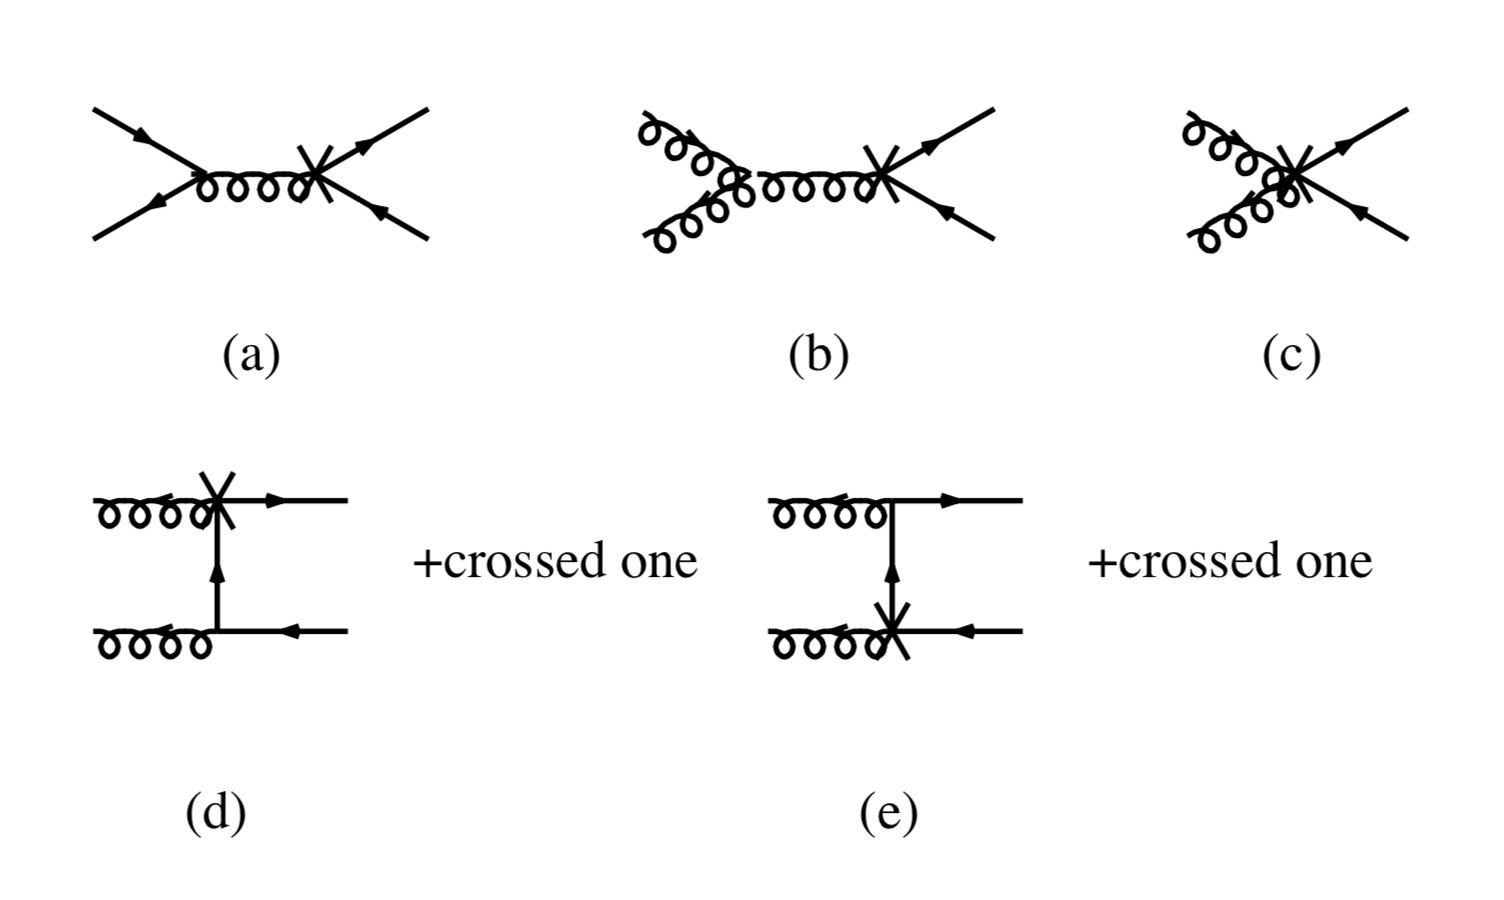
\includegraphics[width=0.85\textwidth]{Figures/Intro/qqgg_tt.png}
		\caption{Tree level Feynman diagram for $qq \rightarrow t\bar{t}$ and $gg \rightarrow t\bar{t}$, the crosses in diagrams denote the vertices modified by top CEDM \cite{Zhou:1998wz}}
		\label{Intro:fig:qqgg_tt}
		\end{figure}
		\FloatBarrier

		After the Higgs boson's discovered and standard model's development, Eq.\ref{eq:CEDM_L_ori} is not appropriate to the gauge invariance and symmetry of standard model. That is to say, any new physics must come in the form of an effective Lagrangian that respects all the symmetries of the SM, in particular the SU(2)(weak interaction) symmetry. This symmetry forbids couplings in Eq.\ref{eq:CEDM_L_ori}. The form of lagrangian in Eq.\ref{eq:CEDM_L_ori} could be reserve but to adapt it, the correct gauge invariant, operators must include a Higgs field. The adaptive form is shown in Eq.\ref{eq:CEDM_L_ada}.

		% adapted L after SM
		\begin{equation}
		\begin{split}
		L_{cdm} = g_s \frac{d_{tG}}{\Lambda^2} \bar{q_3} T^a\sigma^{\mu \nu} t \widetilde{\phi} G^a_{\mu \nu} + H.c.
		\label{eq:CEDM_L_ada}
		\end{split}
		\end{equation}
		\FloatBarrier

		where the $q_3$ is the third generation SM quark doublet, $\widetilde{\phi}$ is the scalar doublet, and the $T^a$ are the SU(3) generators. The relation between $d_{tG}$ and $d_t^g$ is shown(Eq.\ref{eq:CEDM_L_connection}). then the absorptive part of form factor $d_t^g$ which arises from a loop should not be written down in lagrangian.

		\begin{equation}
		\begin{split}
		d_t^g = \frac{\sqrt{2} v}{\Lambda^2} Im(d_{tG})
		\label{eq:CEDM_L_connection}
		\end{split}
		\end{equation}
		\FloatBarrier

		In addition to the CPV from CEDM in production of $t\bar{t}$, there are also CP violation, which is the anomalous couplinng $f$, arise in the vertices of $t\bar{t}$ with the decay $t \rightarrow bW^+$ and $\bar{t} \rightarrow \bar{b}W^-$, and would arise in the vertices of $t\bar{t}$. The $f$ is composed of CP conserving phase $\delta_f$ and CP violating phase $\phi_{f}$ with $\widetilde{f}$ parametrised. The vertices are shown below Eq.\ref{eq:CEDM_CPV_decay}, ref.\cite{PhysRevD.81.034013}:

		\begin{equation}
		\begin{split}
		\Gamma^{\mu}_{W_{tb}} = - \frac{g}{\sqrt{2}}V_{tb}^{*} \bar{u}(p_{b})[ \gamma_{\mu} P_{L} - i\widetilde{f}e^{i(\phi_f + \delta_f)} \sigma^{\mu \nu} (p_t - p_b)_{\nu} P_R ] u(p_t) \\
		\bar{\Gamma}^{\mu}_{W_{tb}} = - \frac{g}{\sqrt{2}}V_{tb} \bar{v}(p_{\bar{t}})[ \gamma_{\mu} P_{L} - i\widetilde{f}e^{i(-\phi_f + \delta_f)} \sigma^{\mu \nu} (p_{\bar{t}} - p_{\bar{b}})_{\nu} P_L ] v(p_{\bar{b}})
		\end{split}
		\label{eq:CEDM_CPV_decay}
		\end{equation}
		\FloatBarrier

		These two CP violating anomalous couplings, $d_t^g$ and $\widetilde{f} \sin{\phi_f}$, have induced the T-odd correlation, so it is considered to using T-odd observables to detecting.(ref.\cite{PhysRevD.81.034013},\cite{PhysRevD.79.013013},\cite{PhysRevD.80.034013}) Besides, there are some probable models could be the source of CP violation in $t\bar{t}$ like 2HDM model. There are some discussion in section. The emphasis of this analysis is to focus on approach to the top CEDM phenomenon.

		% mainly to detect CEDM, theory part of CEDM

	\subsection{Triple product observables to detect CP violation in LHC}
	\label{ssec:Intro_TPinLHC}

		% intro of naive T, T-odd, T-even. focus on T-odd
		% used 4 observables, why? corresponding to detector

		To approach the possibility of CP violation in sample, the time reversal would be introduced because of the assumption of CPT conservation which indicates that all the physical states are the eigenstates of CPT operator in the universe. Therrefore, the observables we used in the analysis are the triple product observables which are exactly $\textbf{T-odd observables}$. The $T$ here means the time reversal operator, more accurately, there is the $\textbf{naive time reversal operator}$ $\textbf{T}_N$. The ordinary time reversal operator means that it changes signs of the momenta and spins of all particles and also exchange the initial and final states. The naive time operator, however, is the time reversal without interchanging between initial state and final state because the initial state's detection and calculations are not available for usual decay process in experiment. That is to say, if the combination of charge and parity is not conserved, the kinematics of final state would tell the CP-violation story. The applied observable -- T-odd triple product observables, which basic form is shown below(Eq.\ref{eq:triple_product_form}):(ref.\cite{PhysRevLett.58.451},\cite{PhysRevD.80.034013}, )

		\begin{equation}
		O = \vec{v_{1}} \cdot ( \vec{v_2} \times \vec{v_{3}} )
		\label{eq:triple_product_form}
		\end{equation}
		\FloatBarrier

		where the $v_{1,2,3}$ are the momentum or spins vectors. It is obvious to be T-odd($T_{N}$-odd) type because of there are three components. Furthermore, there are also some T-even observables but not the usage of this analysis. Also, there are more combinations about these three vector, so CP-odd and CP-even type of triple product might have appeared. The CP-odd(CP-even) means the eigenvalue of CP eigenstate is -1(+1). The prefered triple product observables are commonly the CP-odd observables, take the observable $O = \vec{p_{l^-}} \cdot ( \vec{p_{t}} \times \vec{p_{\bar{t}}} )$ in \cite{PhysRevLett.58.451} for example:

		\begin{equation}
		\begin{split}
		p_{t}\xrightarrow[\text{}]{\text{CP}} -p_{\bar{t}} \; \; , \; \; p_{t}\xrightarrow[\text{}]{\text{CP}} -p_{\bar{t}} \; , \; \; \\
		p_{l^-} \xrightarrow[\text{}]{\text{CP}} p_{l^-} \; \; , \; \; p_{l^-} \xrightarrow[\text{}]{\text{CP}} p_{l^+} \;, \\
		\vec{p_{l^-}} \cdot ( \vec{p_{t}} \times \vec{p_{\overline{t}}} ) \xrightarrow[]{\text{CP}} \vec{p_{l^-}} \cdot ( - \vec{p_{\overline{t}}} \times - \vec{p_{t}} ) \\
		= \vec{p_{l^-}} \cdot ( \vec{p_{t}} \times \vec{p_{\overline{t}}} ) \;\;\;\;\;\;
		\end{split}
		\label{eq:ex_obs_eett}
		\end{equation}
		\FloatBarrier

		where the observable is CP-odd. We only put emphasis on the CP-odd observables. Given a CP-odd observable, we can define an asymmetry measurement in Eq.\ref{eq:asymmetry_form} which is established on counting events between positive and negative value of observable. The $O_i$ in Eq.\ref{eq:asymmetry_form} means the CP-odd observables and different observables have different sensitivity to the CP violation if there is new physics involved.

		\begin{equation}
		A_{cp} = \frac{ N_{events}(O_i>0) - N_{events}(O_i<0) }{ N_{events}(O_i>0) + N_{events}(O_i<0) }
		\label{eq:asymmetry_form}
		\end{equation}
		\FloatBarrier

		% development of triple product observable
		Under the form Eq.\ref{eq:triple_product_form} and the CP-odd design Eq.\ref{eq:asymmetry_form}, we can easily build T-odd observables for detecting CP violation. \\
		
		To discuss about the general case of T-odd triple product observable, there is a simple case -- the $\textbf{inclusive case}$, which is the jets' information used only. The parity operator would change the sign of four momentum, but the charge conjugate could not change the jets' sign because it is summed over by particles and antiparticles in defining the jets. There are 3 jets' momenta ordered by energy or spread by $p_{\perp}$($E_1$>$E_2$>$E_3$ or $p_{\perp 1}$ > $p_{\perp 2}$ > $p_{\perp 3}$). They are also used to form a CP-odd triple product $J$(Eq.\ref{eq:inclusive_obs1}, ref.\cite{PhysRevLett.58.451}):

		\begin{equation}
		J = \vec{p}_1 \cdot \vec{p}_2 \times \vec{p}_3
		\label{eq:inclusive_obs1}
		\end{equation}
		\FloatBarrier

		however, there is a adapted one with beam direction $\vec{p}$ and some total polarization $\vec{S}$ perpendicular to the beam direction. They both are unchange under CP operation, so the rest one is dropped a jet four momentum to make it CP-odd still. The form is shown in Eq.\ref{eq:inclusive_obs2}(ref.\cite{PhysRevLett.58.451}.

		\begin{equation}
		\widetilde{J} = \vec{p}_- \times \vec{S} \cdot \vec{p}_{jet}
		\label{eq:inclusive_obs2}
		\end{equation}
		\FloatBarrier

		Another case is the semi-inclusive process. When the particles identification is improved, the particles is not merely labeled by its four momentum. Therefore, there are wider tests could be adopted to do CP-test, and it is exactly more effective in the modern collider experiments. We denote the flavor of particles as $F$ and their anti-particles as $\bar{F}$, the possible observable terms are shown(Eq.\ref{eq:semi_inclusive_obs},ref.\cite{PhysRevLett.58.451}):

		\begin{equation}
		\begin{split}
		\vec{p}_- \times \vec{p}_{jet} \cdot ( \vec{p}_F - \vec{p}_{\bar{F}} ) \;\;, \;\; \vec{S} \times \vec{p}_{jet} \cdot ( \vec{p}_F - \vec{p}_{\bar{F}} ) \\
		\vec{p}_- \times \vec{S} \cdot ( \vec{p}_F + \vec{p}_{\bar{F}} ) \;\;, \;\; \vec{p}_{jet,1} \times \vec{p}_{jet,2} \cdot ( \vec{p}_F + \vec{p}_{\bar{F}} ) \\
		\vec{p}_- \cdot ( \vec{p}_F \times \vec{p}_{\bar{F}} ) \;\;,\;\; \vec{S} \cdot ( \vec{p}_F \times \vec{p}_{\bar{F}} )
		\label{eq:semi_inclusive_obs}
		\end{split}
		\end{equation}
		\FloatBarrier

		The $(\vec{p}_F + \vec{p}_{\bar{F}})$ in Eq.\ref{eq:semi_inclusive_obs} means the particle and anti-particle are not necessary to be really distinguished, for example, it is acceptible that the charges of 2 same flavor jets are not clearly assigned under the type of observable. On the other hand, the $(\vec{p}_F - \vec{p}_{\bar{F}})$ and $(\vec{p}_F \times \vec{p}_{\bar{F}})$ need more accuracy at seperating particle and anti-particle. Morreover, there is also a CP-odd type but T-even observables like Eq.\ref{eq:3vec_Teven}, but it is not used in this real data analysis. T-even observables will be discussed more in section.\ref{ssec:AcpObs}.

		\begin{equation}
		\vec{p}_{jet} \cdot ( \vec{p}_F - \vec{p}_{\bar{F}} )
		\label{eq:3vec_Teven}
		\end{equation}
		\FloatBarrier

		% related to this analysis

		For the LHC experiment, the proton-proton initial state is not a CP eigenstate. Also, under the LHC's energies, the dominant gluon fusion initial state($gg \rightarrow t\bar{t}$) is not CP eigen state, either. However, summing over gluon's flavors and colors could achieve CP-odd observables which in the similar way as the jets observables. There are three channel for $t\bar{t}$ decay -- hadronic channel, leptonic channel, and single lepton+jets channel. The hadronic channel presents both of W bosons decay to two jets respectively, and the leptonic channel assumes both of W boson decay to lepton and neutrino which is detected as Missing $E_T$ in analysis. The analysis is to probe CP violation in $t\bar{t}$ semileptonic decay Eq.\ref{eq:semileptonic_decay}, where both top quarks decay to bottom quarks and W bosons. Then one of W bosons decays and ends up with being recognized as 2 jets($j_1$,$j_2$), and the other one decays to lepton and neutrino. All of suitable observables for each channel are researched in ref.\cite{PhysRevD.80.034013},\cite{PhysRevD.81.034013},\cite{Hayreter:2015ryk}.

		\begin{equation}
		t\bar{t} \rightarrow b\bar{b} W^+W^- \rightarrow b\bar{b} jj l \nu
		\label{eq:semileptonic_decay}
		\end{equation}
		\FloatBarrier

		There are more organized T-odd triple product observables in ref.\cite{Hayreter:2015ryk} for leptonic channel and single lepton+jets channel. Yet, there are some constraint to make it valid in real experiments. For instance, the $O_1$ in\cite{Hayreter:2015ryk} is $\epsilon(p_t,p_{\bar{t}},p_b,p_{\bar{b}}) = \epsilon_{\mu \nu \rho \zeta}p_t^{\mu}p_{\bar{t}}^{\nu}p_b^{\rho}p_{\bar{b}}^{\zeta} \xrightarrow[]{t\overline{t}CM} \vec{p_t} \cdot ( \vec{p_b} \times \vec{p_{\overline{b}}} )$, where the $\epsilon$ is the Levi–Civita tensor and $p_i^{\alpha}$ is the four momentum of i particle. The $p_t$ in $O_1$ have to be reconstructed with information from detector, and the neutrino's z-direction's(collided beam's direction) information could be missed in detector.

		According to the final states' resolution and reconstruction, there are four appropriate observables:

		\begin{equation}
		\begin{split}
		O_3 = Q_l \epsilon(p_{b}, p_{\bar{b}}, p_{l}, p_{j_1}) \xrightarrow[\text{}]{b \bar{b} CM} Q_l \vec{p_{b}} \cdot ( \vec{p_l} \times \vec{p_{j_1}} ) \\
		O_{6} = Q_l \epsilon(P, p_{b}-p_{\bar{b}}, p_{l}, p_{j_1}) \xrightarrow[\text{}]{lab} Q_l (\vec{p_{b}} - \vec{p_{\overline{b}}}) \cdot ( \vec{p_l} \times \vec{p_{j_1}} ) \\
		O_{12} = q \cdot (p_{b}-p_{\bar{b}}) \epsilon(P_{}, q, p_{b}, p_{\bar{b}}) \xrightarrow[]{lab} (\vec{p_{b}} - \vec{p_{\overline{b}}})_z ( \vec{p_b} \times \vec{p_{\overline{b}}} )_z \\
		O_{14} = \epsilon(P, p_{b}+p_{\bar{b}}, p_{l}, p_{j_1}) \xrightarrow[]{lab} (\vec{p_{b}} + \vec{p_{\overline{b}}}) \cdot ( \vec{p_l} \times \vec{p_{j_1}} )
		\end{split}
		\label{eq:four_obs}
		\end{equation}
		\FloatBarrier

		The $j_1$ is the leading $p_T$ jets except the chosen b-flavor jets; $l$ refers to muon or electron, and $Q_l$ is the electric charge of lepton $l$; Also, the $\rightarrow$ and the text above indicates the spacetime frame chose to observe the properties. All the four observables are confirmed CP-odd and available in counting events asymmetry(Eq.\ref{eq:asymmetry_form}). 

		\begin{equation}
		\begin{split}
		\vec{p}_b \overset{CP}{\longleftrightarrow} -\vec{p}_{\overline{b}}\;\;, \;\; \vec{p}_{l^-} \overset{CP}{\longleftrightarrow} -\vec{p}_{l^+}\;\;,\;\;\;\;\;\; \\
		\vec{p}_{j_1} \overset{CP}{\longleftrightarrow} -\vec{p}_{j_1}\;\;, \;\; Q_{l^+} \overset{CP}{\longleftrightarrow} -Q_{l^+} = Q_{l^-}
		\label{eq:CP_rule}
		\end{split}
		\end{equation}
		\FloatBarrier

		Following the CP operator's effect(Eq.\ref{eq:CP_rule}), take $O_6$ for example, the $\mu^+$ is from the case with $W^+$ is leptonic decay and $\mu^-$ is from the case with $W^-$ is leptonic decay(Eq.\ref{eq:O6ex}), it is exactly CP-odd:

		\begin{equation}
		\begin{split}
		O_6 = Q_l (\vec{p}_b - \vec{p}_{\bar{b}}) \cdot (\vec{p}_{\mu^-} \times \vec{p}_{j_1} + \vec{p}_{\mu^+} \times \vec{p}_{j_1}) \\
		\xrightarrow[]{CP} -Q_l (\vec{p}_{\bar{b}} - \vec{p}_b) \cdot (-\vec{p}_{\mu^+} \times \vec{p}_{j_1} + -\vec{p}_{\mu^-} \times \vec{p}_{j_1}) = -O_6
		\label{eq:O6ex}
		\end{split}
		\end{equation}
		\FloatBarrier

	\subsection{Experimental and data analysis strategy}
	\label{ssec:Intro_ExpDAStr}

		To really do the experiment to measure the CP violation in $t\bar{t}$, we use the dataset which is collected from $\textbf{Compact Muon Solenoid(CMS)}$ experiment in $\textbf{Large}$ $\textbf{Hadron}$ $\textbf{Collider(LHC)}$ under the institute $\textbf{European}$ $\textbf{Organisation}$ $\textbf{for}$ $\textbf{Nuclear}$ $\textbf{Research}$$\textbf{(CERN)}$. The simple concept of designing of CMS experiment's detector would be introduced in Chapter.\ref{sec:ExperimentalAppratus}. Moreover, the intermediate dealing with raw data to physical objectecs is necessary. The detail of physical objects reonstruction and the object selection will be shown in Chapter.\ref{sec:PhysObj}. As following, the analyzed data and simulation data will be represented in Chapter.\ref{sec:DataAndMC}. There are not only the real data taking shown, but also the simulated data's calibration and correction mentioned.

		It is the primary analysis part to extract the signal from all the messy data. Therefore, the Chapter.\ref{sec:EventSelReco} will tell the techniques to select the events and to reconstruct the confident fragment, and then to tell the probed part. In this analysis, we mainly compare the data and simulation with the invariant mass of top which decays hadronically to validate that our selected data is under a high confidence level of what we want. The objects kinematics and flavor information would be used to events selection, and the known top quark mass and W boson mass informations would be included to help distinguish the selected objects. In addition, the machine learning concept is added in the analysis to help discerning physical objects in final states. After selecting and reconstructing the events, the background, which means the events we have no interest on, should be ruled out although it stands less portion of all the events. The fitting skills would be adopted and the details are in Chapter.\ref{sec:BkgEst}. 

		The reconstruction and detector bias in the measurements play an critical roll because it is not quite direct to measure the physical object in CMS experiment. Chapter.\ref{sec:AsymBias} will discuss how the measurement affected by the reconstrruction and detector issue, also it will discuss how the observables react on the asymmetry measurement. The dilution effect from detector issue to calculation of $A_{cp}$ will discussed in Chapter.\ref{sec:Dilution}. Last but not least, there must be systematic uncertainty considered in any experiments. Chapter.\ref{sec:Systematic} demonstrate the systematic undertainty and their implementation.

		The baseline is mostly similar to the CMS run1's analysis(8TeV)\cite{Khachatryan:2016ngh}. There are some improvement of analysis input in the part of events selection and physical objects distinguishment with MVA tool. Therefore, one of the point we focus in this analysis is to compare the result of using original method($\chi^2_{min}$) and using new method(MVA) to distingusih the physical objects. Also, there are some research on the possible source(model) of CP violation in $t\bar{t}$, and the T-even observables' discussion are listed in the Chapter.\ref{sec:AcpModelObs}.

		The part of conclusion(Chapter.\ref{sec:Result}) collects the results in any chapters and organizes to be final results. There are comparison of method, precision of measurement, and the explanation of the demonstrated informations.


\FloatBarrier

\newpage
% !TEX root = main.tex

% TODO:
%   * Acronym to be covered: \sqrt{s}, $pp$
%   * Make a reference to post-run-I appendix
% REMARK:
% . * LHC, CMS are both defined in this section

\clearpage
\section{Experimental Apparatus}
\label{sec:ExperimentalAppratus}
% http://www.lhc-closer.es/taking_a_closer_look_at_lhc/1.lhc_parameters
% https://home.cern/resources/faqs/facts-and-figures-about-lhc

	\subsection{Large Hadron Collider(LHC)}
	\label{ssec:ExpApp_LHC}

	\subsection{Compact Muon Solenoid(CMS) Detector}
	\label{ssec:ExpApp_CMS}

		The CMS use the right-handed system, the x-axis point to the center of LHC, y-axis point up and orthogonal to the ground, and z-axis is along with anti-clockwise beam direction.

		\subsubsection{Magnetic configuration}
		\label{sssec:ExpApp_magnetic}


		\subsubsection{Tracking system}
		\label{sssec:ExpApp_tracking}

			The CMS tracker's schematic drawing is shown below in Fig.\ref{PhysObj:fig:tracker} from reference\cite{Chatrchyan:2014fea} where $\textbf{strip tracker}$ with small silicon tracker within. 

			\begin{figure}[H]
			\centering{}
		    	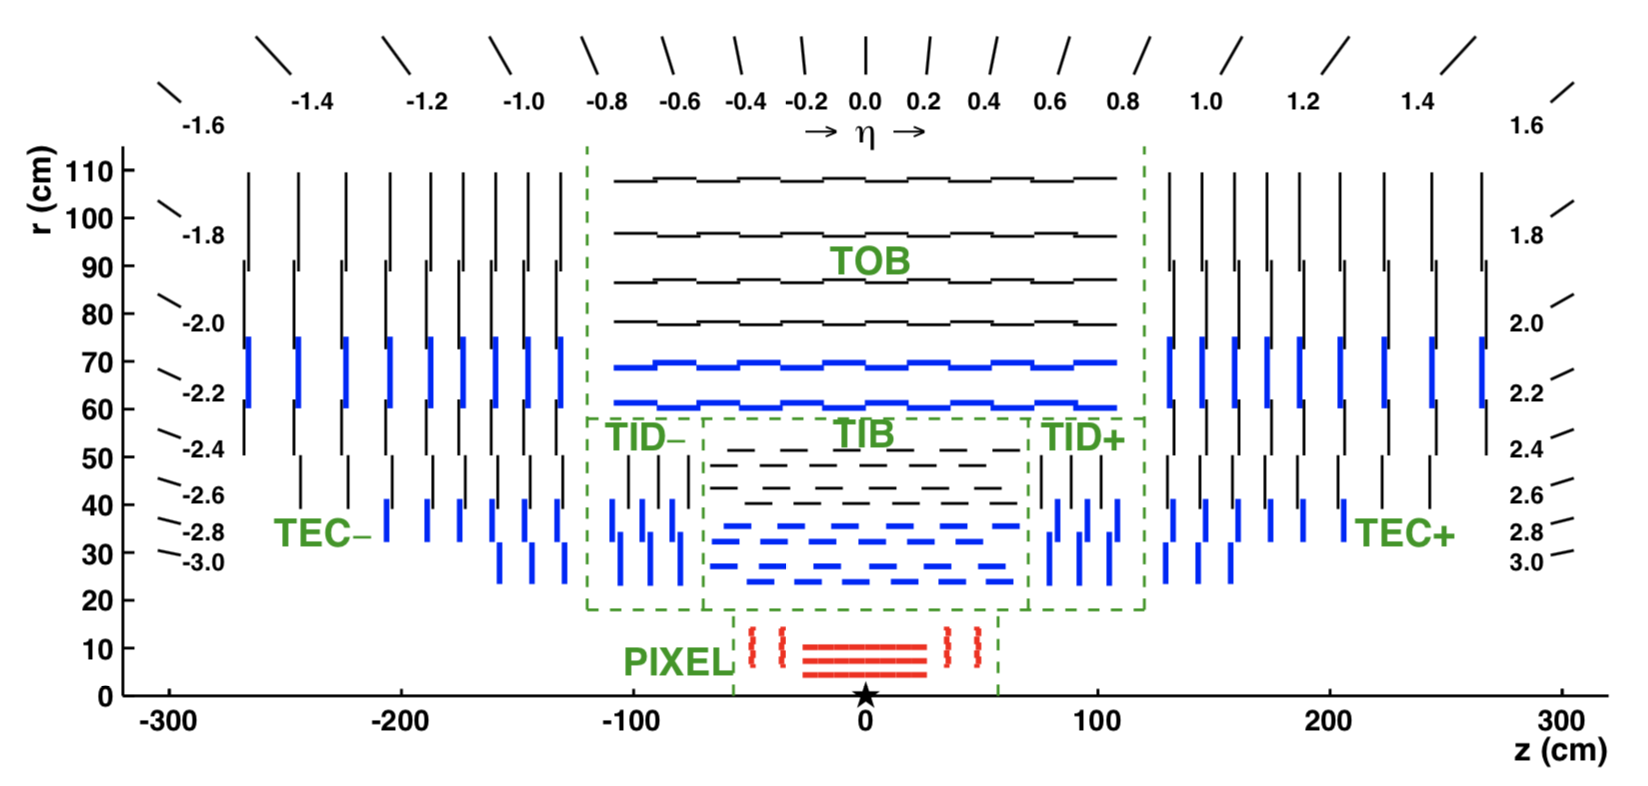
\includegraphics[width=0.85\textwidth]{Figures/ExpApparatus/tracker.png}\\
			\caption{The drawing of the CMS inner tracking system\cite{Chatrchyan:2014fea}}
			\label{PhysObj:fig:tracker}
			\end{figure}
			\FloatBarrier

			Futhermore, the tracker is immersed in magnetic field from CMS solenoid. There are four subsystem in it and they are completed by endcaps(|pseudorapidity $\eta | < 2.5$) on either sides of barrels. The four subsystems are the $\textbf{Tracker Inner Barrel (TIB)}$, the $\textbf{Tracker Inner Disk (TID)}$, the $\textbf{Tracker Outer Barrel(TOB)}$, and the $\textbf{Tracker EndCaps(TEC)}$. There are slices of silicons in these tracking subsystems, and the detail of thickness, position and layers would be found in reference\cite{Chatrchyan:2014fea}. Also, the summary of the principal characteristics of the various tracker subsystems from \cite{Chatrchyan:2014fea} is attached below:
			
			\begin{figure}[H]
			\centering{}
		    	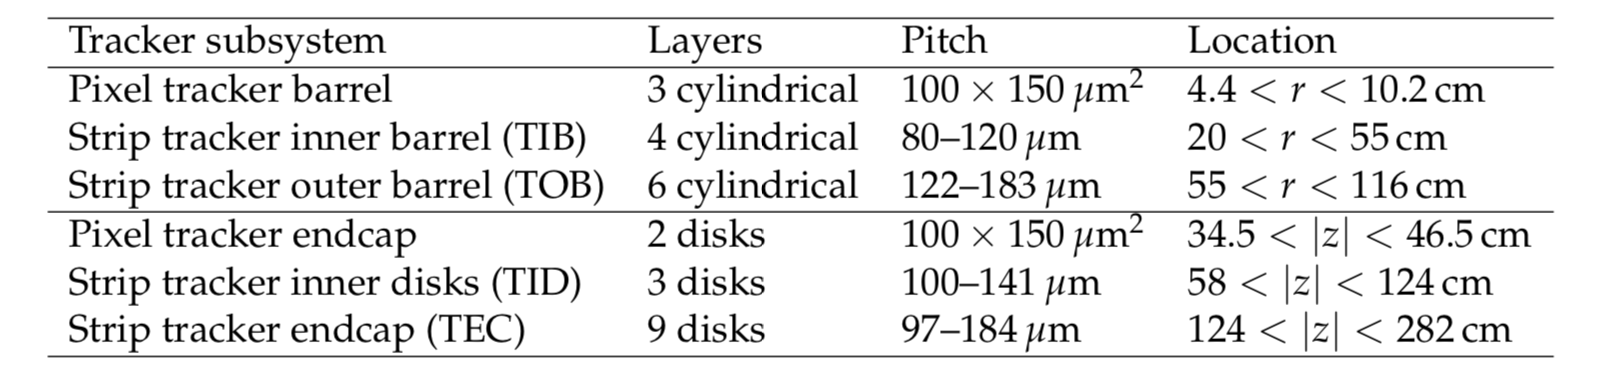
\includegraphics[width=0.85\textwidth]{Figures/ExpApparatus/summary_subtracker.png}\\
			\caption{Summary of the principal characteristics of the various tracker subsystems\cite{Chatrchyan:2014fea}}
			\label{PhysObj:fig:tracker_sum}
			\end{figure}




	%including apparatus and simulator(mg5,pyhtia,delphes)
\newpage
% !TEX root = main.tex

% TODO:
% REMARK:

\section{Physical Objects Reconstruction and Selection}
\label{sec:PhysObj}

	\subsection{Vertex}
	\label{ssec:PhysObj_vertex}

		% https://iopscience.iop.org/article/10.1088/1742-6596/110/9/092009/pdf

	\subsection{Pileup Issue}
	\label{ssec:PhysObj_pu}{}

		% https://cms.cern/news/reconstructing-multitude-particle-tracks-within-cms
		Because of the high luminosity of pp collision in CMS, there are more than one pp collision occuring in every time when the the bunches cross one another. The multiple collision in one crossing event is called $\textbf{pile-up(pileup)}$. In the present, the LHC is operating at an instantaneous luminosity of $0.7\times10^{34} cm^{-2}s^{-1}$, and the proton bunches cross inside CMS every 50 ns, so there are more proton in one bunch and showing high pileup. Also, the high granularity and efficiency of CMS Tracker make them distinguish the many tracks in an event. The pileup image is shown below(Fig.\ref{PhysObj:fig:pileup_img}).

		% https://cms.cern/news/reconstructing-multitude-particle-tracks-within-cms
		\begin{figure}[H]
		\centering{}
	    	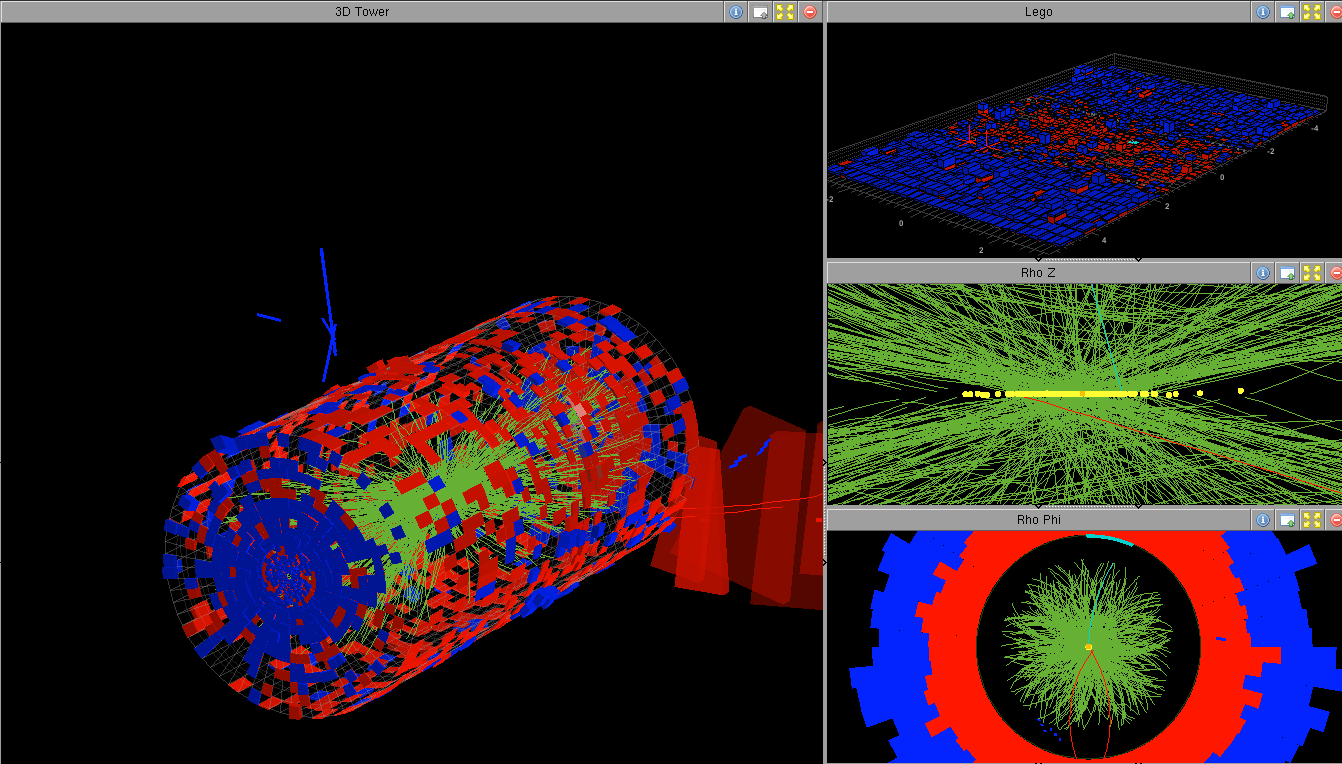
\includegraphics[width=0.85\textwidth]{Figures/PhysObj/pileup_image.png}\\
		\caption{78 reconstructed vertices in one crossing from high pileup run (3D, lego, on Pho-z plane, on Rho-Phi plane)}
		\label{PhysObj:fig:pileup_img}
		\end{figure}
		\FloatBarrier



	\subsection{Lepton}
	\label{ssec:PhysObj_lep}

		The selected lepton in the analysis is required to obey the criteria of one passed $\emph{selected lepton}$ and zero $\emph{veto lepton}$ passed. The veto criteria means that there would be no lepton passing the veto criteria except the selected one. In other words, the veto criteria can filter the physical objects which are lepton-like but not really like after reconstructed from particle level to detector level. The selected criteria corresponds to tight lepton's criteria, and veto criteria follows loose lepton's criteria:

		\subsubsection{Muon}
		\label{sssec:Muon}
			

		\subsubsection{Electron}
		\label{sssec:Electron}

	\subsection{Jet}
	\label{ssec:PhysObj_jet}

		\subsubsection{B-tagged jet}
		\label{sssec:bjet}


	\subsection{Trigger}
	\label{ssec:PhysObj_trg}





\FloatBarrier

\newpage
% !TEX root = main.tex

% TODO:
% REMARK:

\section{Data and Simulation samples}
\label{sec:DataAndMC}

	\subsection{Data sample}
	\label{ssec:DataAndMC_Data}

	% remember to mention golden json

	\subsection{Simulation sample}
	\label{ssec:DataAndMC_MC}

	\subsection{Correction on simulation sample}
	\label{ssec:DataAndMC_corMC}

		% pileup introduction is set on "vertex"
		\subsubsection{Pile-up Reweighing}
		\label{sssec:DataAndMC_PU}

			% https://twiki.cern.ch/twiki/bin/viewauth/CMS/PileupMCReweightingUtilities?fbclid=IwAR0SuZFQ5Um0IfZn1-CHXia6NPMYe2_7cz2OGXxhCYvNvfl_tTBke-w22l8

			As mention in section.\ref{ssec:PhysObj_pu}, pileup is the issue that bunch of vertices occuring at one collision. Although Monte Carlo sample may roughly cover the pileup interactions, the final distribution is also sensitive to the subtle content of primary vertex. Furthermore, the distribution of reconstructed vertices can be differently affected by the offline event selection cut and some high level trigger between real data and Monte Carlo sample. To fix the descrepancy between data and simulation, with any pileup number(number of primary vertices) bin, we compare the data and MC distribution and get the data/MC value bin by bin. The gotten scale factors under pileup number bins will be applied on the analyzed MC to correct the weight of each event.

		\subsubsection{Jet Energy correction, smearing and resolution}
		\label{sssec:DataAndMC_JE_CSR}

			The JEC and JER are mentioned in section.\ref{ssec:PhysObj_jet} previously.

		\subsubsection{Lepton efficiency Scale Factor}
		\label{sssec:DataAndMC_LepEffSF}

		With selection cut or quality pick-up on physics objects like leptons, there must be difference in the selection performance between data and MC. To correct the discrepancy, the often method is apply a scale factor on the $p_T$-$\eta$ space to correct the weight of this event. The scale factor S.F. is calculated from selection efficiency performance of known data and MC by Eq.\ref{eq:eff_SF}. 

		\begin{equation}
		S.F. = \frac{\epsilon_{data}(p_T,\eta)}{\epsilon_{MC}(p_T,\eta)}
		\label{eq:eff_SF}
		\end{equation}

		It is usually implemented by tag-and-probe method\cite{tagandprobe_twiki}. There are efficiency S.F. of muonISO, muonID, muonTrigger, ElectronReco, ElectronID, and ElectronTrigger necessary to be considered. The gotten scale factors under $p_T$-$\eta$ space are shown below:

		\begin{figure}[H]
			\centering
			    \subfigure[Muon ISO]{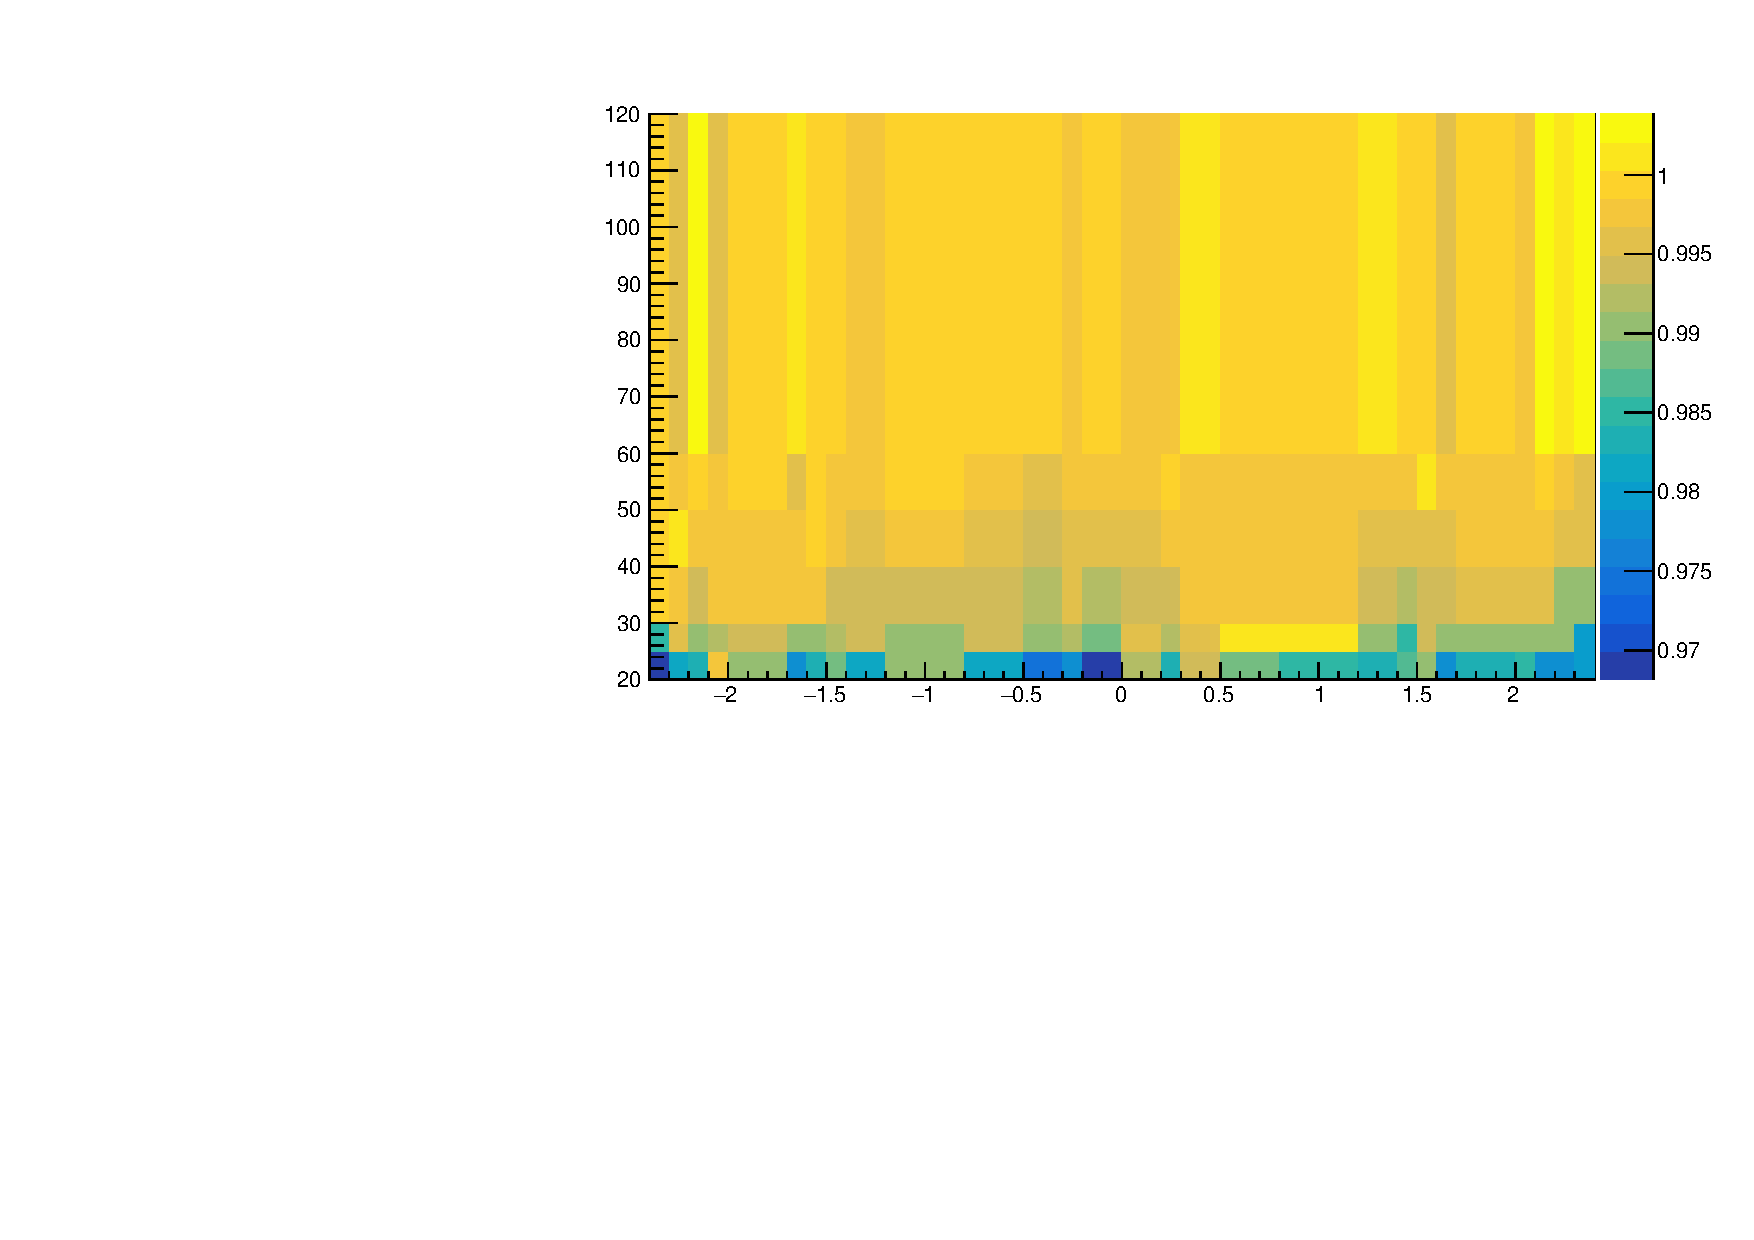
\includegraphics[width=0.32\textwidth]{Figures/DataMC/mu_ISO.pdf}}
			    \subfigure[Muon ID]{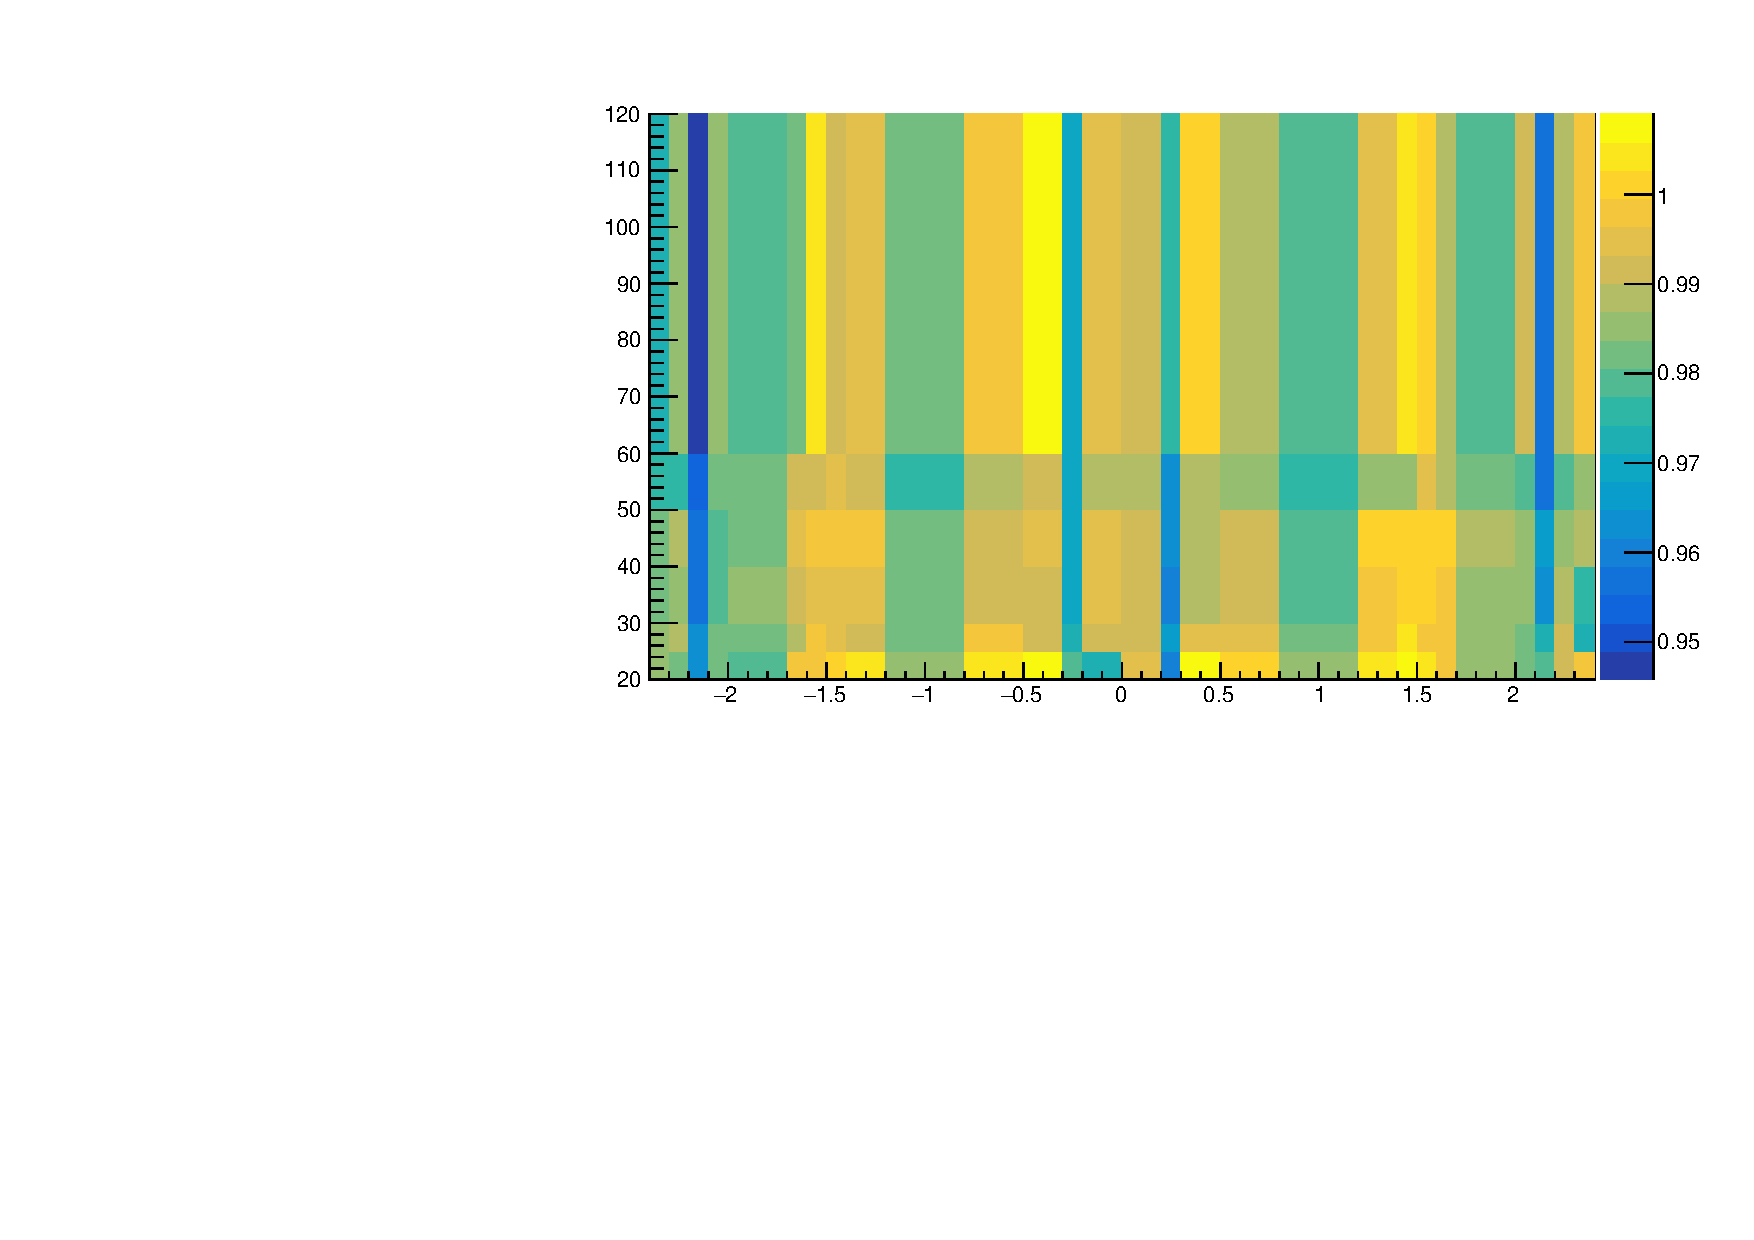
\includegraphics[width=0.32\textwidth]{Figures/DataMC/mu_ID.pdf}}
			    \subfigure[Muon High Level Trigger]{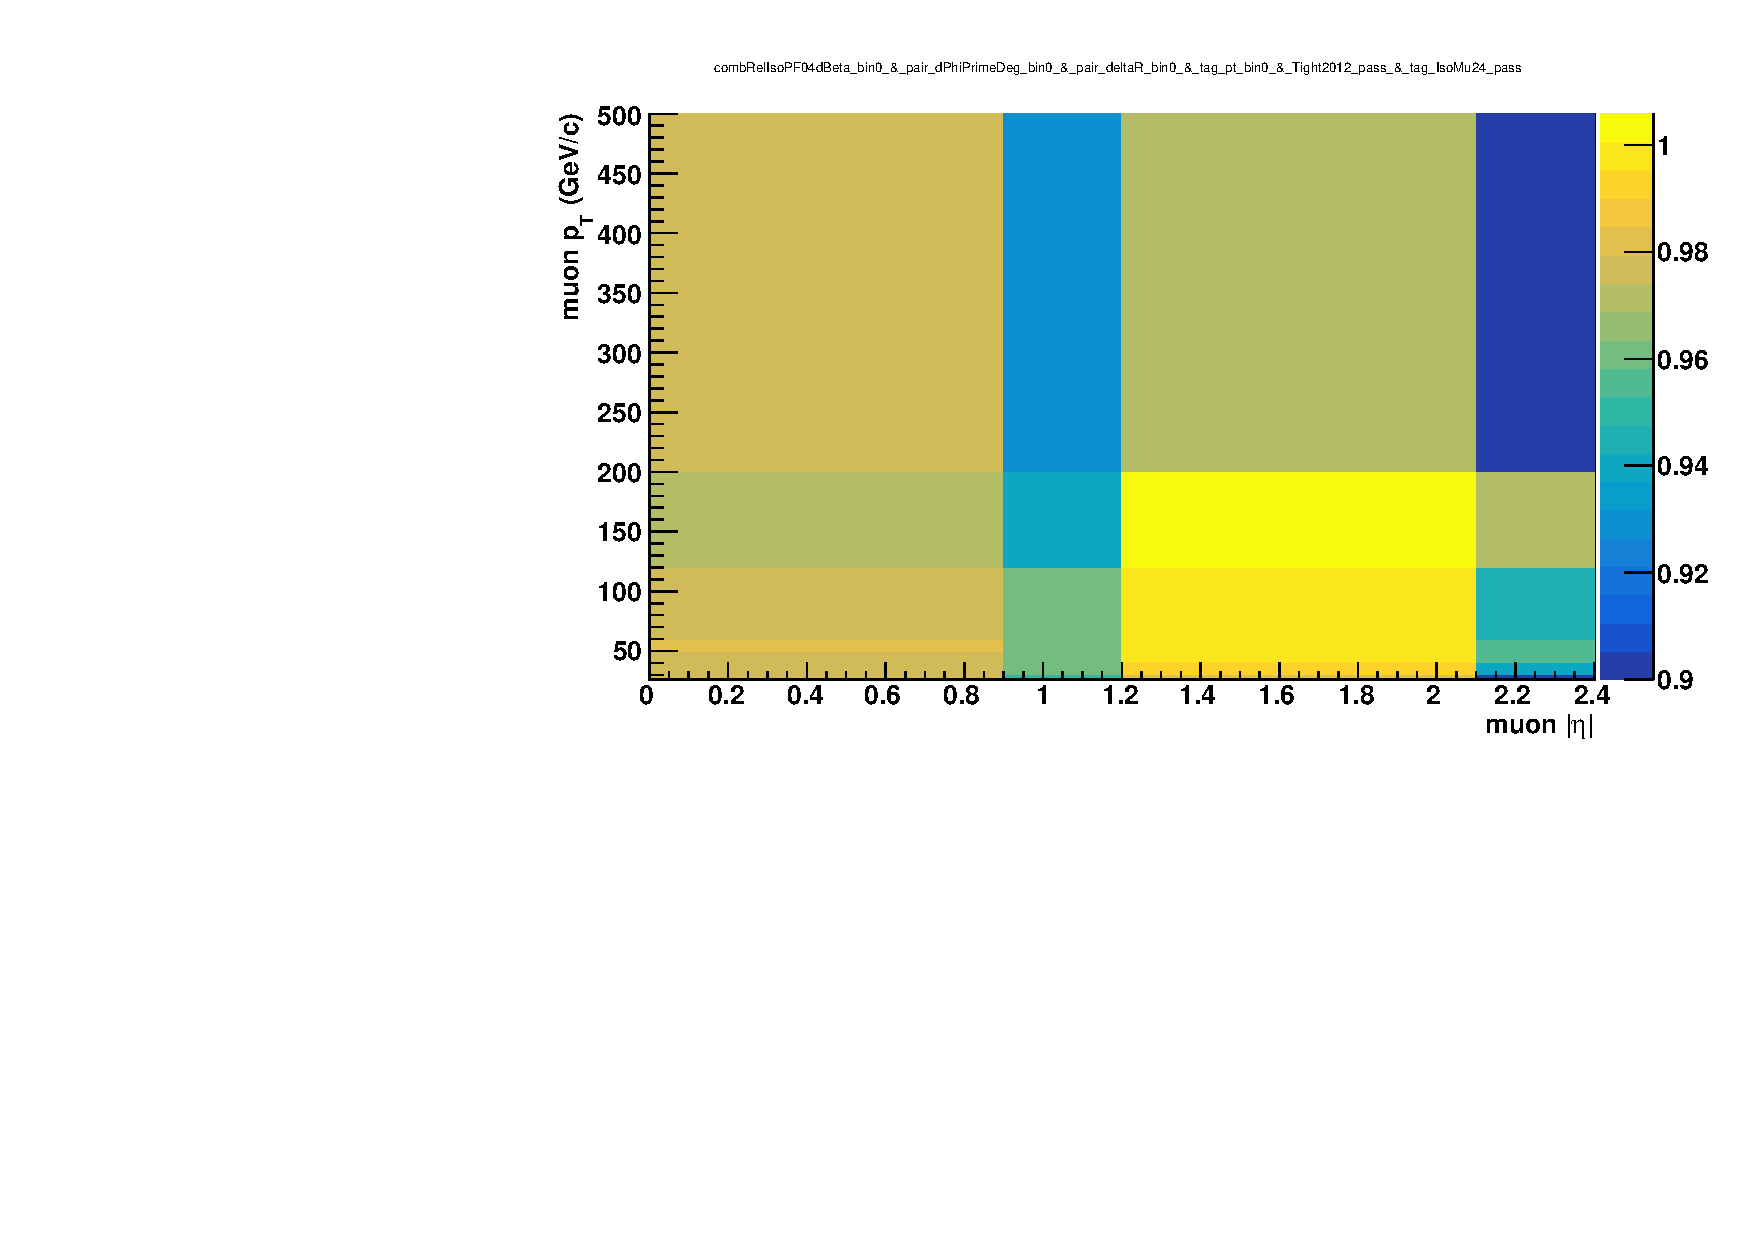
\includegraphics[width=0.32\textwidth]{Figures/DataMC/mu_Trg.pdf}}\\
			\end{figure}
			\FloatBarrier
			\begin{figure}[H]
			\centering
			    \subfigure[Electron Reco]{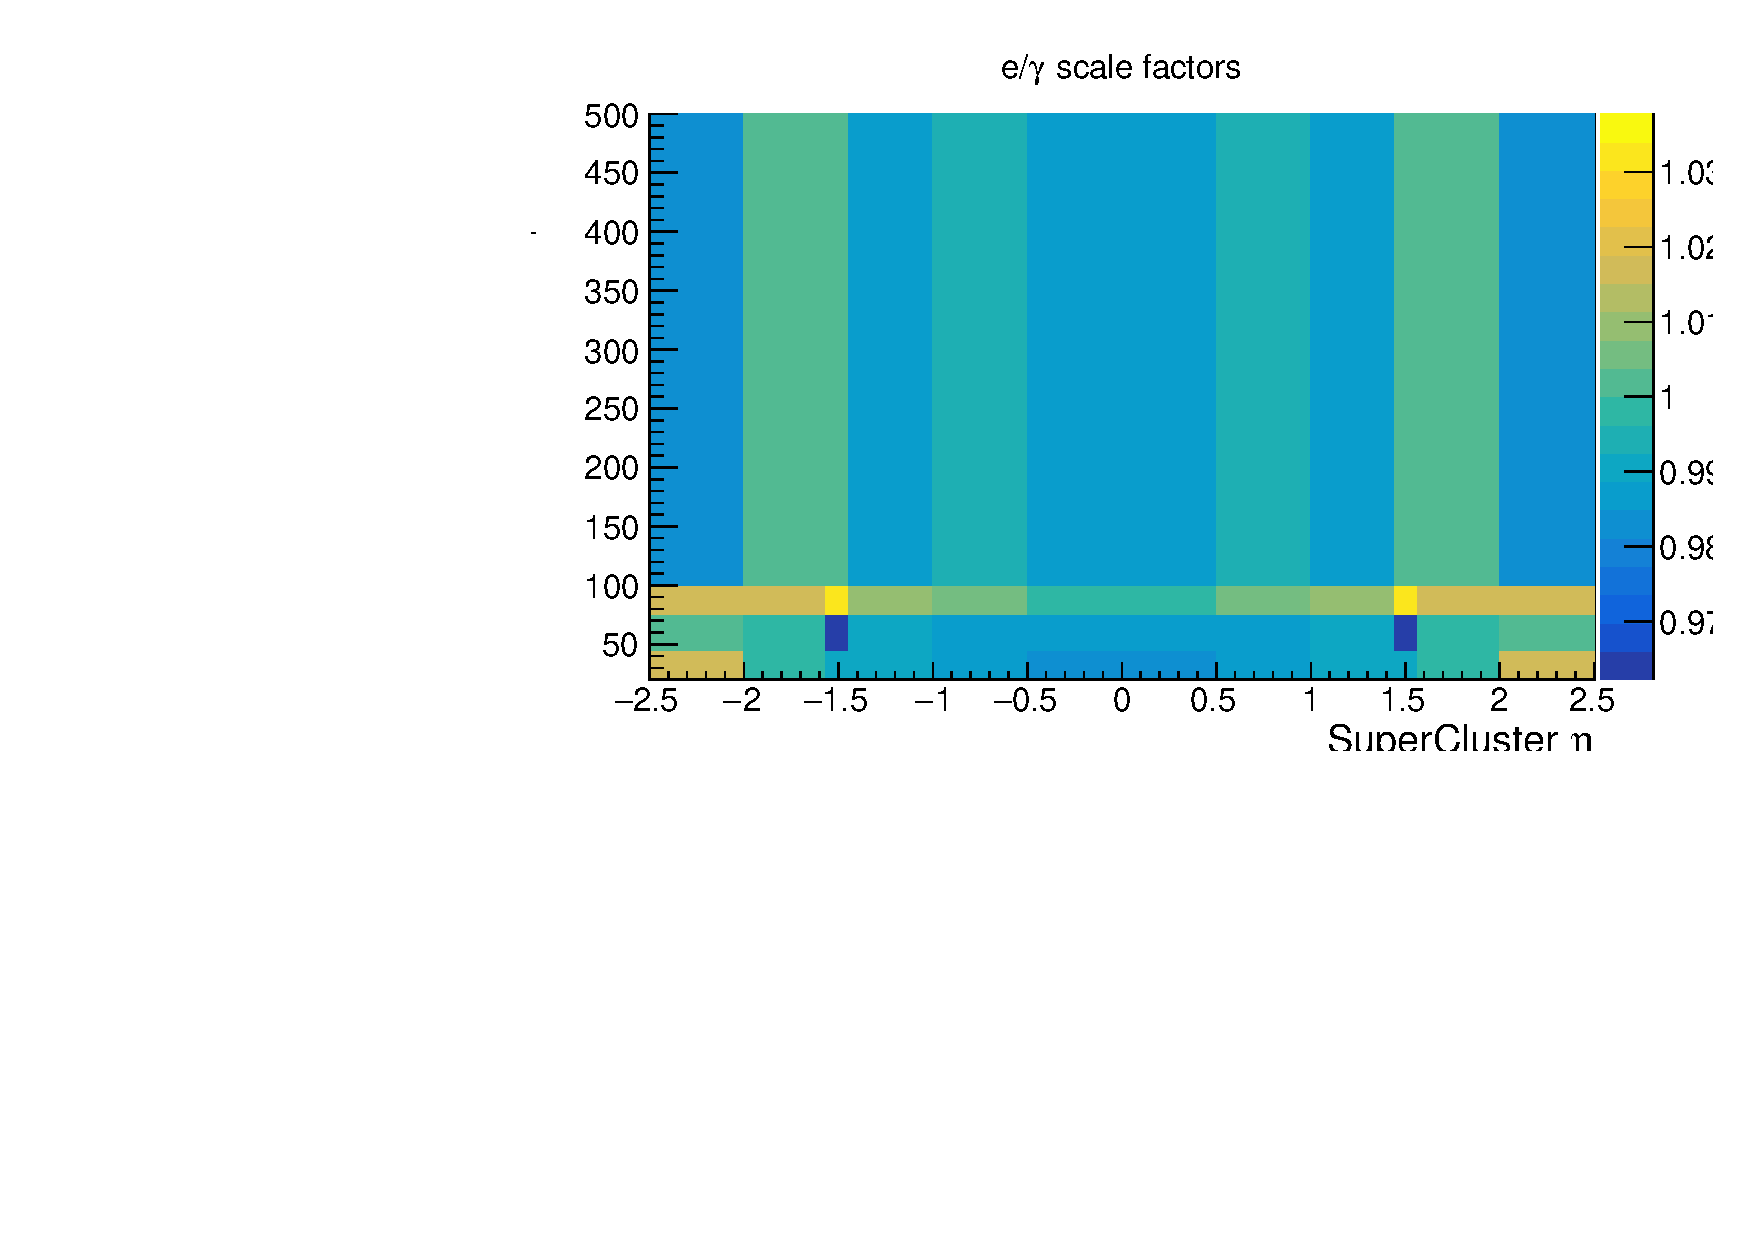
\includegraphics[width=0.32\textwidth]{Figures/DataMC/el_Reco.pdf}}
			    \subfigure[Electron ID]{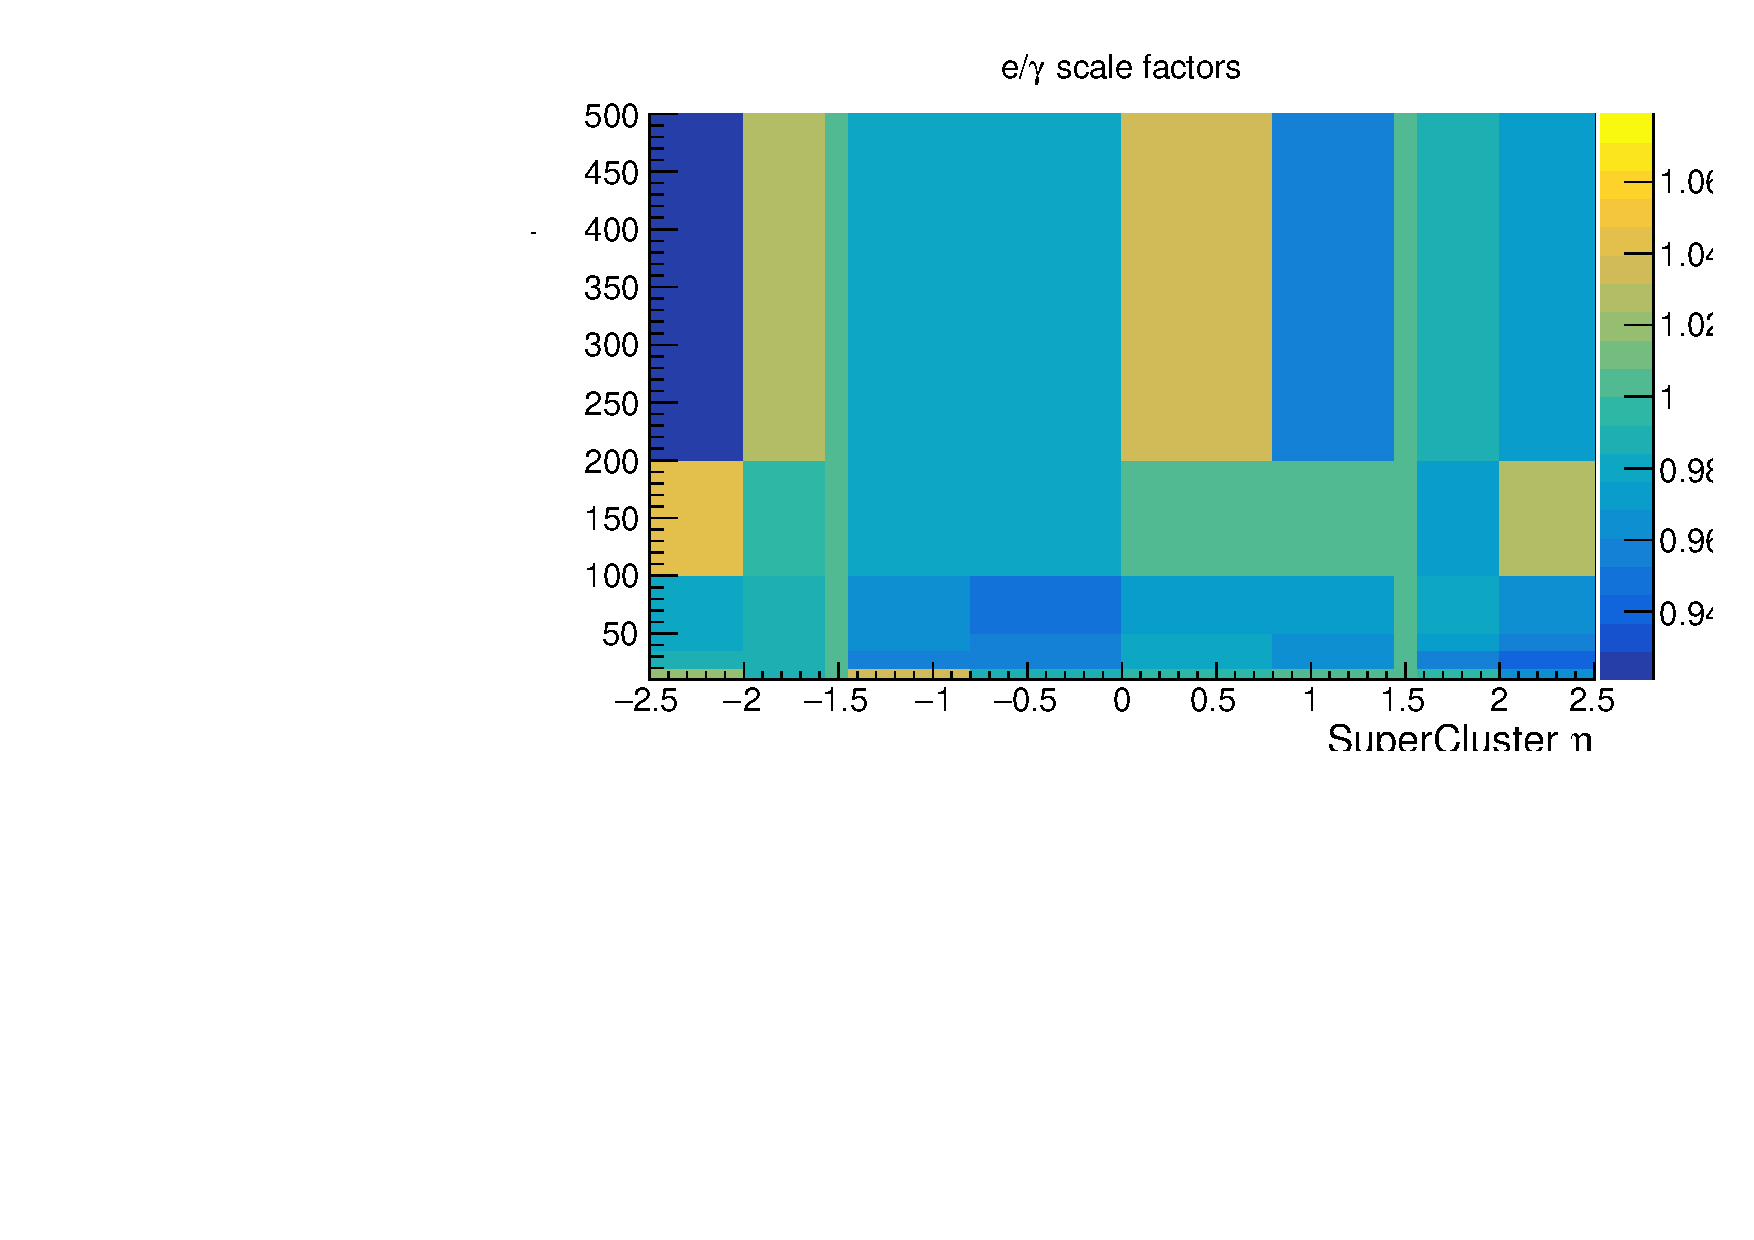
\includegraphics[width=0.32\textwidth]{Figures/DataMC/el_ID.pdf}}
			    \subfigure[Electron High Level Trigger]{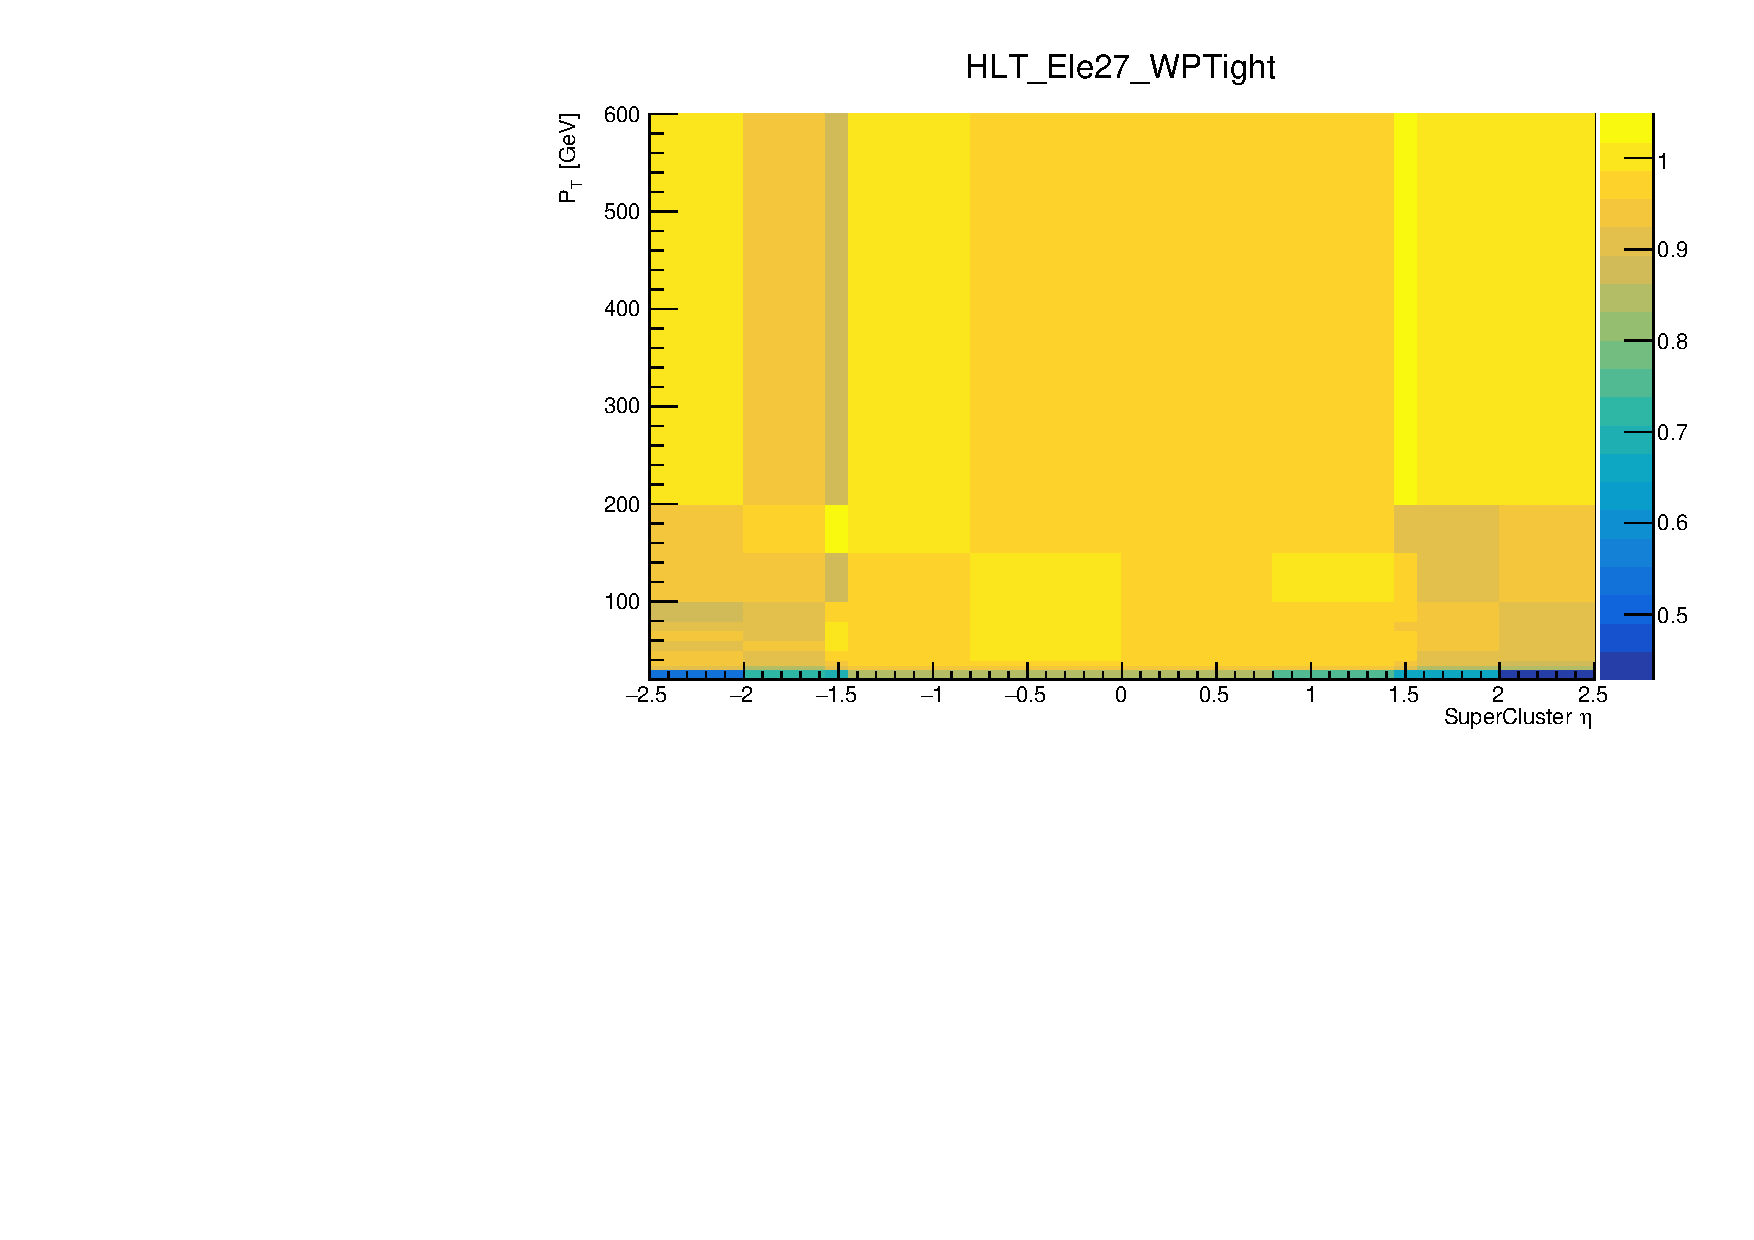
\includegraphics[width=0.32\textwidth]{Figures/DataMC/el_Trg.pdf}}\\
			   \caption{Lepton efficiency scale factor (x-axis:$\eta$, y-axis:$p_T$)}
			\label{DataMC:fig:lepsf}
			\end{figure}
			\FloatBarrier

		\subsubsection{b-tagging Scale Factor}
		\label{sssec:DataAndMC_btagSF}

		The btag scale factor complies with the same concept as efficiency scale factor. Because of applying the selection which is deepCSV cut (DeepCSV Medium and DeepCSV Loose), data and MC have different performance on selection efficiency. 



		\subsubsection{Weigh to Luminosity}
		\label{sssec:DataAndMC_lumi}




%%%--- TODO ---%%%
%%% table of the MC sample's Xsec and generated events number and generator -> weight to luminosity

\begin{center}
\begin{tabular}{ c c c c c }
\hline
Process sample & Cross Section (pb) & k-factor & Events Number & Generator \\ 
\hline
$t$$\bar{t}\rightarrow b \bar{b}jjl\nu$ & XXX & 1 & CCCCCC & AAAAAA \\
\hline
cell7 & cell8 & XXXXXX & cell7 & cell8 \\
\hline  
\end{tabular}
\end{center}


\FloatBarrier

\newpage
% !TEX root = main.tex

% TODO:
% REMARK:
% . * Don't mention LHC, CMS, etc. in this section, just have a historical review ana provide physical motivation to the study

\section{Events Selection and Reconstruction}
\label{sec:EventSelReco}

	To calculate the asymmetry from top quark in $t\bar{t}$, there must be some selections to extract the $t\bar{t}$ sample from other background samples. Also, there would be several analysis strategies to recognize physical objects and pick them out. The chapter will do these discussion and make some comparison and organization.

	In this analysis, doing reasearch by the channel of lepton + jets, which means 2 tops have different decay modes. One decays leptonically, and another decays hadronically(they will be called $\emph{hadronic top}$ and $\emph{leptonic top}$ in following context). It is expected that the hadronic top can be constructed with 1 b-tagged jet and 2 non b-tagged jets and the other top can be constructed imcompletely with 1 b-tagged jet, 1 lepton with missing neutrino 4-momentum by detector issue. 
	
	\subsection{Trigger}
	\label{ssec:EvtSel_trg}

		In addition to L1 online trigger mentioned in \ref{ssec:PhysObj_trg}, there are also offline trigger here to filter specific events. It's called $\textbf{High Level Trigger(HLT)}$. It's a software trigger usually filter events with kinematics like energy($E$), invariant mass($M$), transverse momentum($p_{T}$), etc. With final states including one selected isolated lepton in this analysis, if they are unprescaled during the entire data collecting, single lepton triggers are chose. For both 2016 data and MC, there are the HLT we use on SingleMuon and SingleElectron sample individually:

		\begin{itemize}
	  		\item $\textbf{Single Muon}$: $\emph{HLT IsoMu24 \textbf{or} HLT IsoTkMu24}$, which pick out events whose muon with reconstructed $p_{T}$ > 24 GeV, or track reconstructed muons with reconstructed $p_{T}$ > 24 GeV.
	  		\item $\textbf{Single Electron}$: $\emph{HLT Ele27 WPTight}$, which pick out events whose electron with reconstructed $p_{T}$ > 27 GeV.
	  	\label{EventSelReco:itm:HLT}
		\end{itemize}

		% https://twiki.cern.ch/twiki/bin/view/CMS/MuonHLT
		% https://twiki.cern.ch/twiki/bin/view/CMS/EgHLTRunIISummary

	\subsection{Events Selection : Signal Region}
	\label{ssec:EvtSel_SR}

		For the $\textbf{Signal Region(SR)}$, the region with selection cut to extract signal in an analysis, there are the selection cuts below, with the physical objects' criteria menntioned in Chapter.\ref{sec:PhysObj}:

		\begin{itemize}
	  		\item 1 selected lepton which are a tight muon or a tight electron
	  		\item 0 lepton pass veto criteria which are loose muon and loose electron criterion
	  		\item $\geq$ 4 selected jets with passing medium jet criteria
	  		\item exact 2 btagged jets(deepCSV Medium criteria) in these selected jets
	  		\item each selected jets are isolated from the selected lepton with $\Delta R$ > 0.4
	  	\label{EventSelReco:itm:full_sel}
		\end{itemize}

		The $\Delta R$ criteria here means the angle distribution between selected jets and selected lepton in $\phi - \eta$ phase space with $\Delta R$ > 0.4. This would avoid the confusing cases that the lepton is really coming from jets or that the jets have some correlation with lepton in reconstruction process... etc.

		\begin{equation}
		\Delta R = \sqrt{ (\eta_{jet} - \eta_{lep})^2 - (\phi_{jet} - \phi_{lep})^2 } > 0.4
		\end{equation}

		Under SR selection to extract the semi-leptonic $t\bar{t}$(signal), and also following the high level trigger, they are shown in muon and electron channels to classify the selected sample in the following analysis.

		%%% also put on the diagrams of N_Jets N_BJets N_TightLep before selection to valify the selection cut!

		%%% --- TODO --- %%%
		% to do the lumi-weight things (?)

	\subsection{Events Reconstruction}
	\label{ssec:EvtReco}

		To reconstruct the semi-leptonic $t\bar{t}$ system, it is suggested that to reconstruct the hadronic top quark. It's an advantage that we can avoid dealing with missing 4-momentum from neutrino decays from leptonic top. And under the SR selection, if we can reconstruct the top which decays hadronically, the decay objects of leptonic decay top would be picked up simultaneously. This is a direct and common way to correctly identify selected candidates.

		\subsubsection{$\chi^2_{min}$ Method}
		\label{sssec:minchi2_intro} 

			There are multiple combinations of 1 b-tagged jet and 2 non b-tagged jet in an event. And how do we reconstruct hadronic top? In known and published analysis, based on the reco-level invariant mass of top quark itself and the intermediate particle in decay - W boson, they are used as constraints to invariant mass which is reconstructed from each combination. With the defined $\chi^2_{min}$ value, which shows below:

			\begin{equation}
			\chi^2 = (\frac{m_{jjb}-m_{t}}{\sigma_{t}})^2 + (\frac{m_{jj}-m_{W}}{\sigma_{W}})^2
			\label{eq:chi2}
			\end{equation}
			where $m_{t}$, $m_{W}$, $\sigma_{t}$ and $\sigma_{W}$ are the mean and width of top quark and W boson, coming from artificial fitting with jets corresponding to real decay quark with generator information in simulation sample(in appendix****), which are 168.15GeV, 81.25GeV, 20.6GeV and 12.1GeV seperately. Back to the part of $\chi^2$, for each combination, $m_{jjb}$ is the invariant mass of 1 b-tagged jet and 2 non-btagged jets; $m_{jj}$ is the invariat mass of 2 non b-tagged jets which are same 2 jets in $m_{jjb}$. the combination who have the minimum ${\chi}^{2}$ value in all of them is chosen as physical obsects coming from hadronically decay top.


\begin{figure}[H]
\centering
	\subfigure[muon channel]{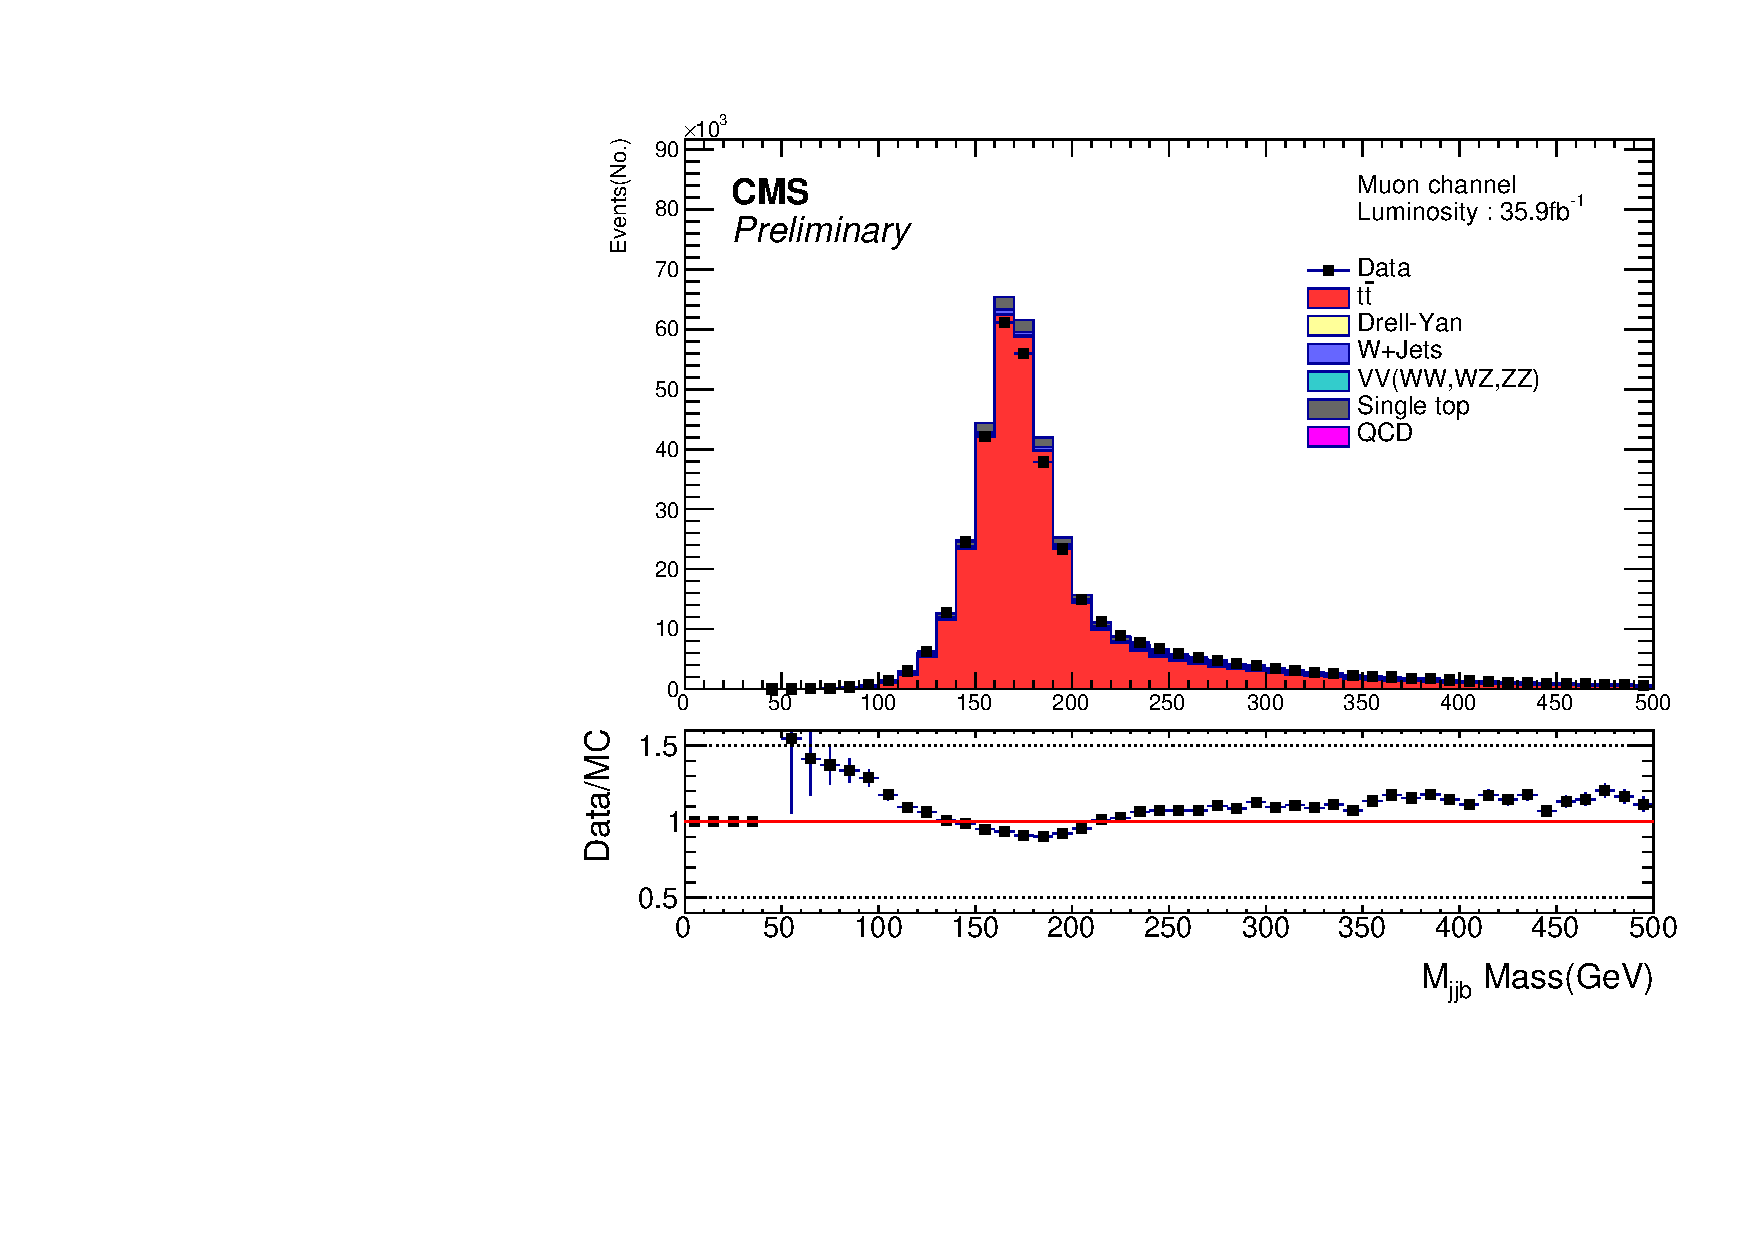
\includegraphics[width=0.45\textwidth]{Figures/EventSelReco/Mass/chi2/chi2_NC_long_HadTop_mu.pdf}}
    \subfigure[electron channel]{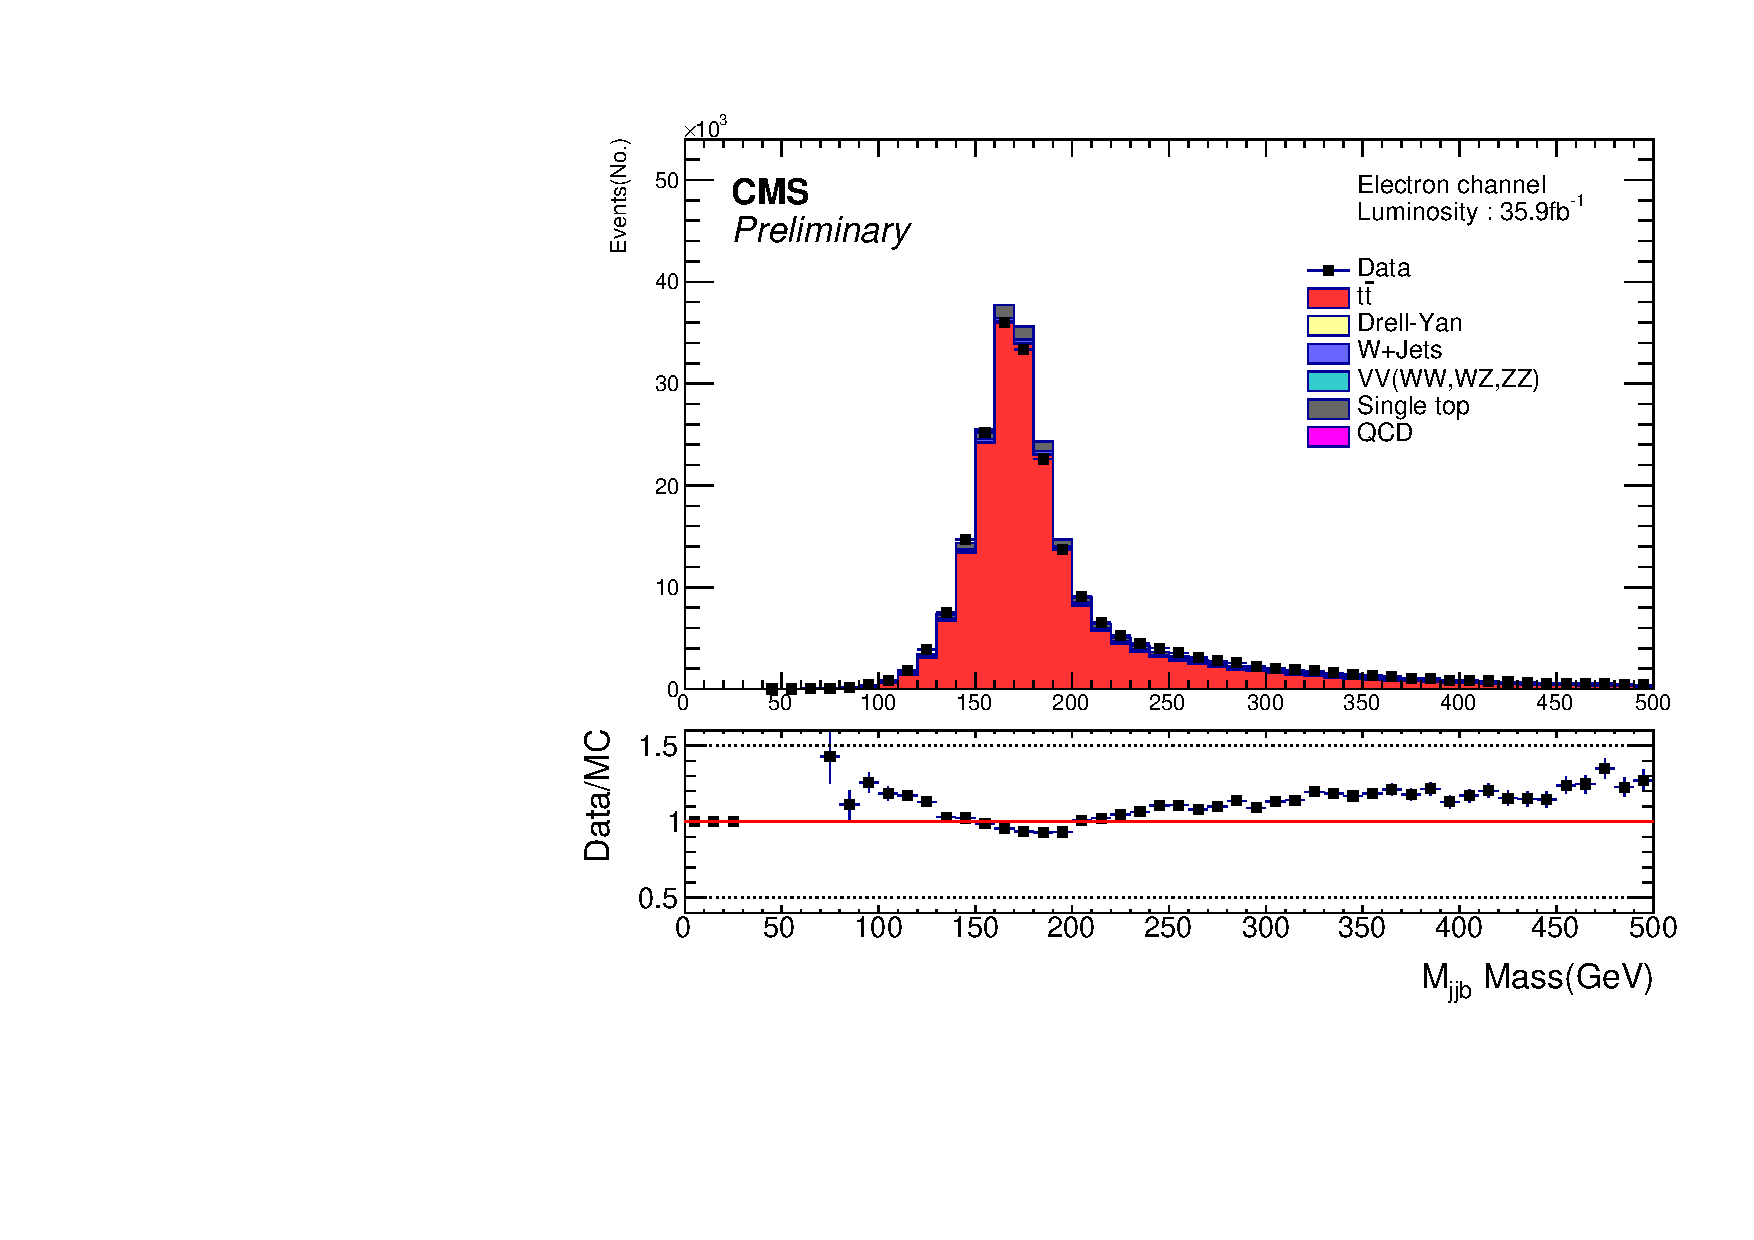
\includegraphics[width=0.45\textwidth]{Figures/EventSelReco/Mass/chi2/chi2_NC_long_HadTop_el.pdf}}\\
\caption{Reconstructed $M_{jjb}$ with $\chi^2_{min}$ algorithm (w/o cut)}
\label{EventSelReco:fig:chi2_SR_NC_Mjjb}
\end{figure}
\FloatBarrier

		\subsubsection{MVA Method}
		\label{sssec:mva_intro} 

			However, to improve the reconstruction performance in my analysis, there is another method - $\textbf{Multi-Variate Analysis (MVA)}$ can be adopted to do well in this reconstruction part. It has been not a common way to used in this step yet compared to signal and background samples' classification. In order to check the improvement between usual and new method, in the following rest analysis, the comparison of analysis results of $\chi^2_{min}$ method and MVA method will be shown simultaneously. 

			The concept of MVA is to use basic machine learning method to classify signal and background, we'll take advantage of MVA discriminating ability to improve the correctness rate of selection compared with $\chi^2_{min}$ method.
				
			As the usage of classification, one should define the $"$signal$"$ and $"$background$"$ in MVA configuration. In most particle physics analysis with MVA, $"$signal$"$ means the physics sample which is expected to be analyzed and as a target sample and the $"$background$"$ means samples from the other known physics. Different as usual, in this analysis,

			\begin{itemize}

				\item $\textbf{Sample}$ : signal simulation sample($t\bar{t}$ MC) with full event selection(\ref{ssec:EvtSel_SR})
				\item Randomly half for training sample, another half for testing sample
				\item In each event,
				\begin{enumerate}
					\item $\textbf{Signal}$ is recognized as the correct combination of objects hadronically decaying from $t$($\bar{t}$)-quark in an event
					\item $\textbf{Background}$ are all the other incorrect combinations in an event
				\end{enumerate}
			\end{itemize}

			To identify whether one combination is the 2 jets and the correct detector-level's objects from generator-level's particles, the $\Delta R$ method is used to match them. The matching method is to compare the angle distribution between detector-level objects and generator-level particles with $\Delta R$ < 0.4. 
			
			\begin{equation}
			\Delta R = \sqrt{ (\eta_{det} - \eta_{gen})^2 - (\phi_{det} - \phi_{gen})^2 } < 0.4
			\label{eq:gen_matching}
			\end{equation}
		
			With concept of machine learning, we need to train with informations of classes( $"$signal$"$ and $"$backgroud$"$ in this case ) and get out an algorithm to make distinguishment. Following the original $\chi^2_{min}$ method's variables, we started MVA with inputting 2 variables : $m_{jj}$, $m_{jjb}$, as informations to be used for distinguishment. There are three machine learning methods I used for testing: $\textbf{MLP}$(ANN, Artificial Neuro-Network), $\textbf{BDT}$(Boosted Decision Tree), $\textbf{BDTG}$(Boosted Decision Tree Gradient).

			With respect to the input variables for distinguishment training, we can check the seperation shows on input variables originally in advance:

			\begin{figure}[H]
			\centering{}
    			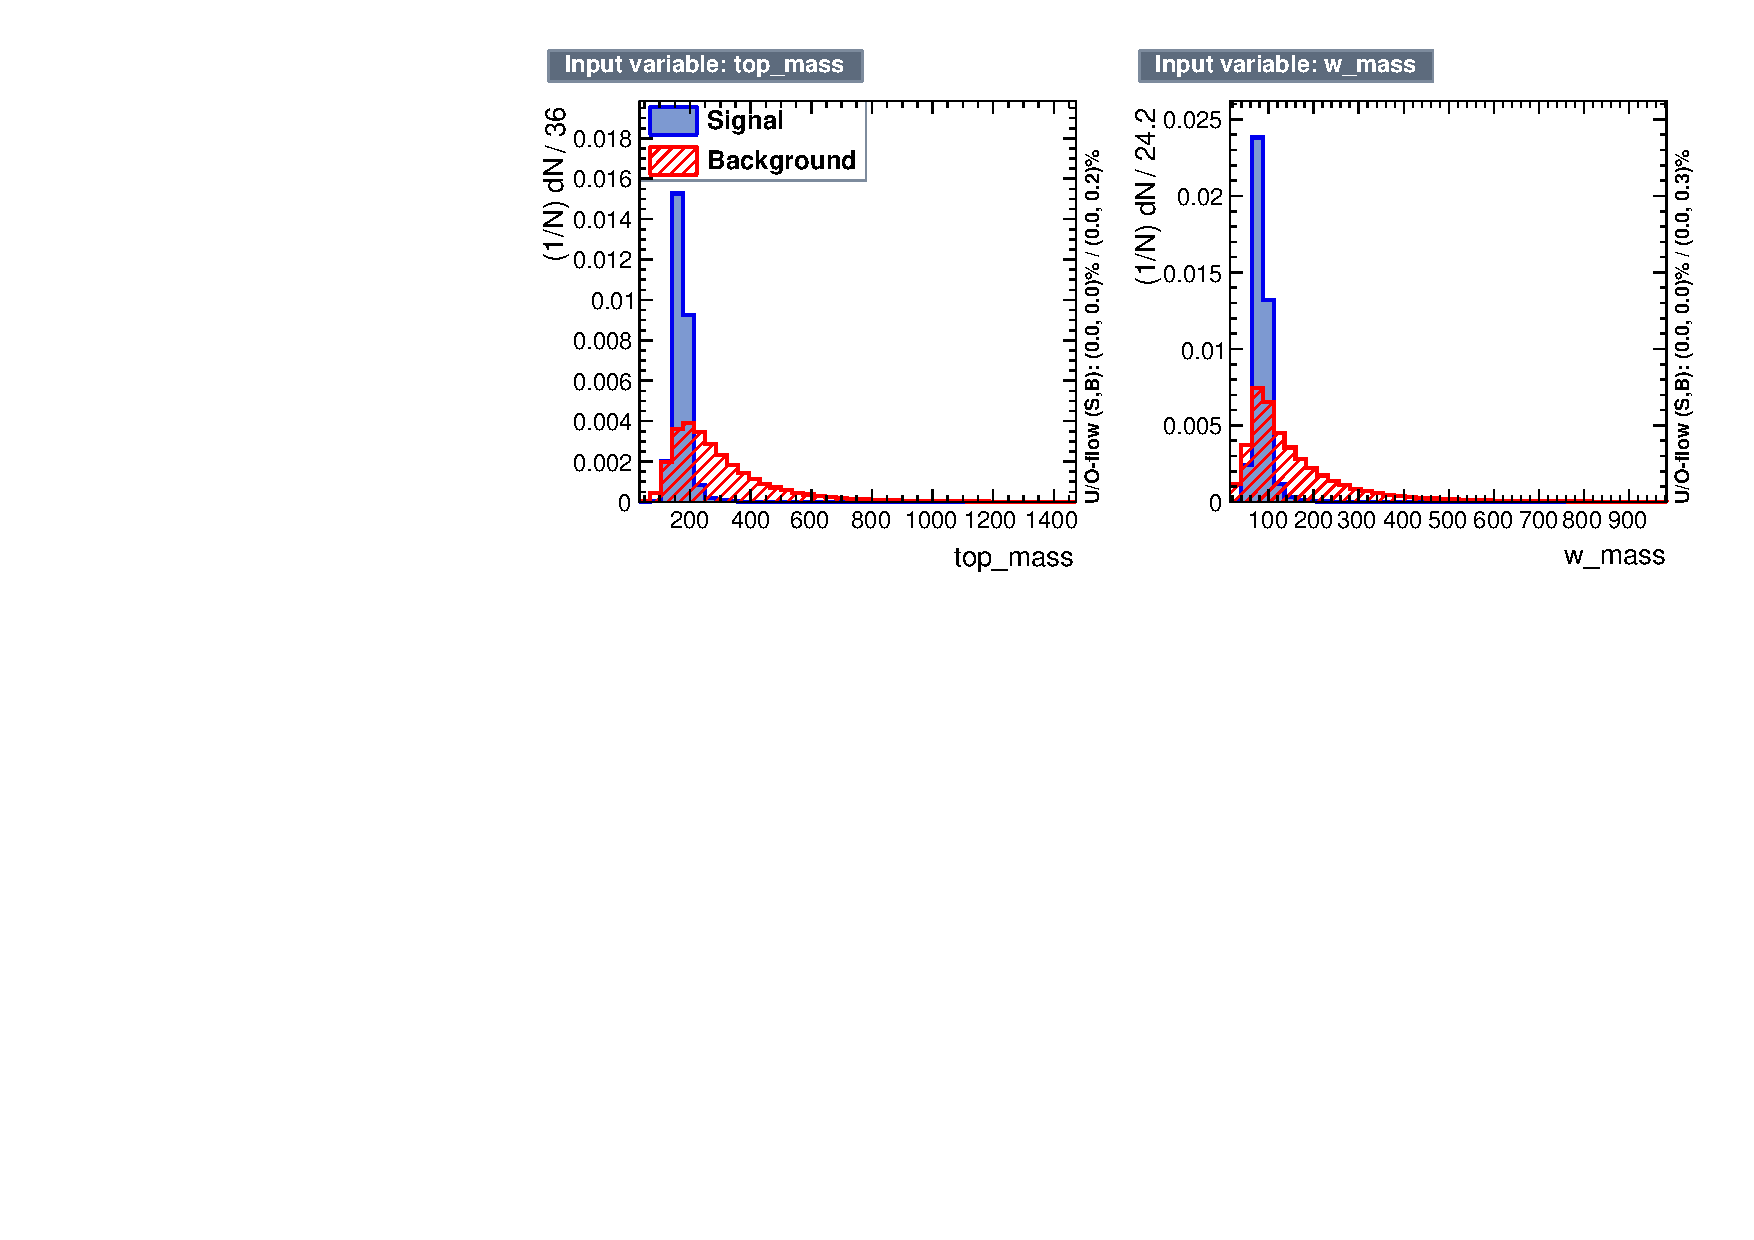
\includegraphics[width=0.85\textwidth]{Figures/EventSelReco/mva/a04_VarSep.pdf}\\
			\caption{Input training variables separation between $"$signal$"$ and $"$background$"$.(2 variables)}
			\label{EventSelReco:fig:a04_varsep}
			\end{figure}
			\FloatBarrier

			And the training result shows below:

			\begin{figure}[H]
			\centering
				\subfigure[BDT's separation result]{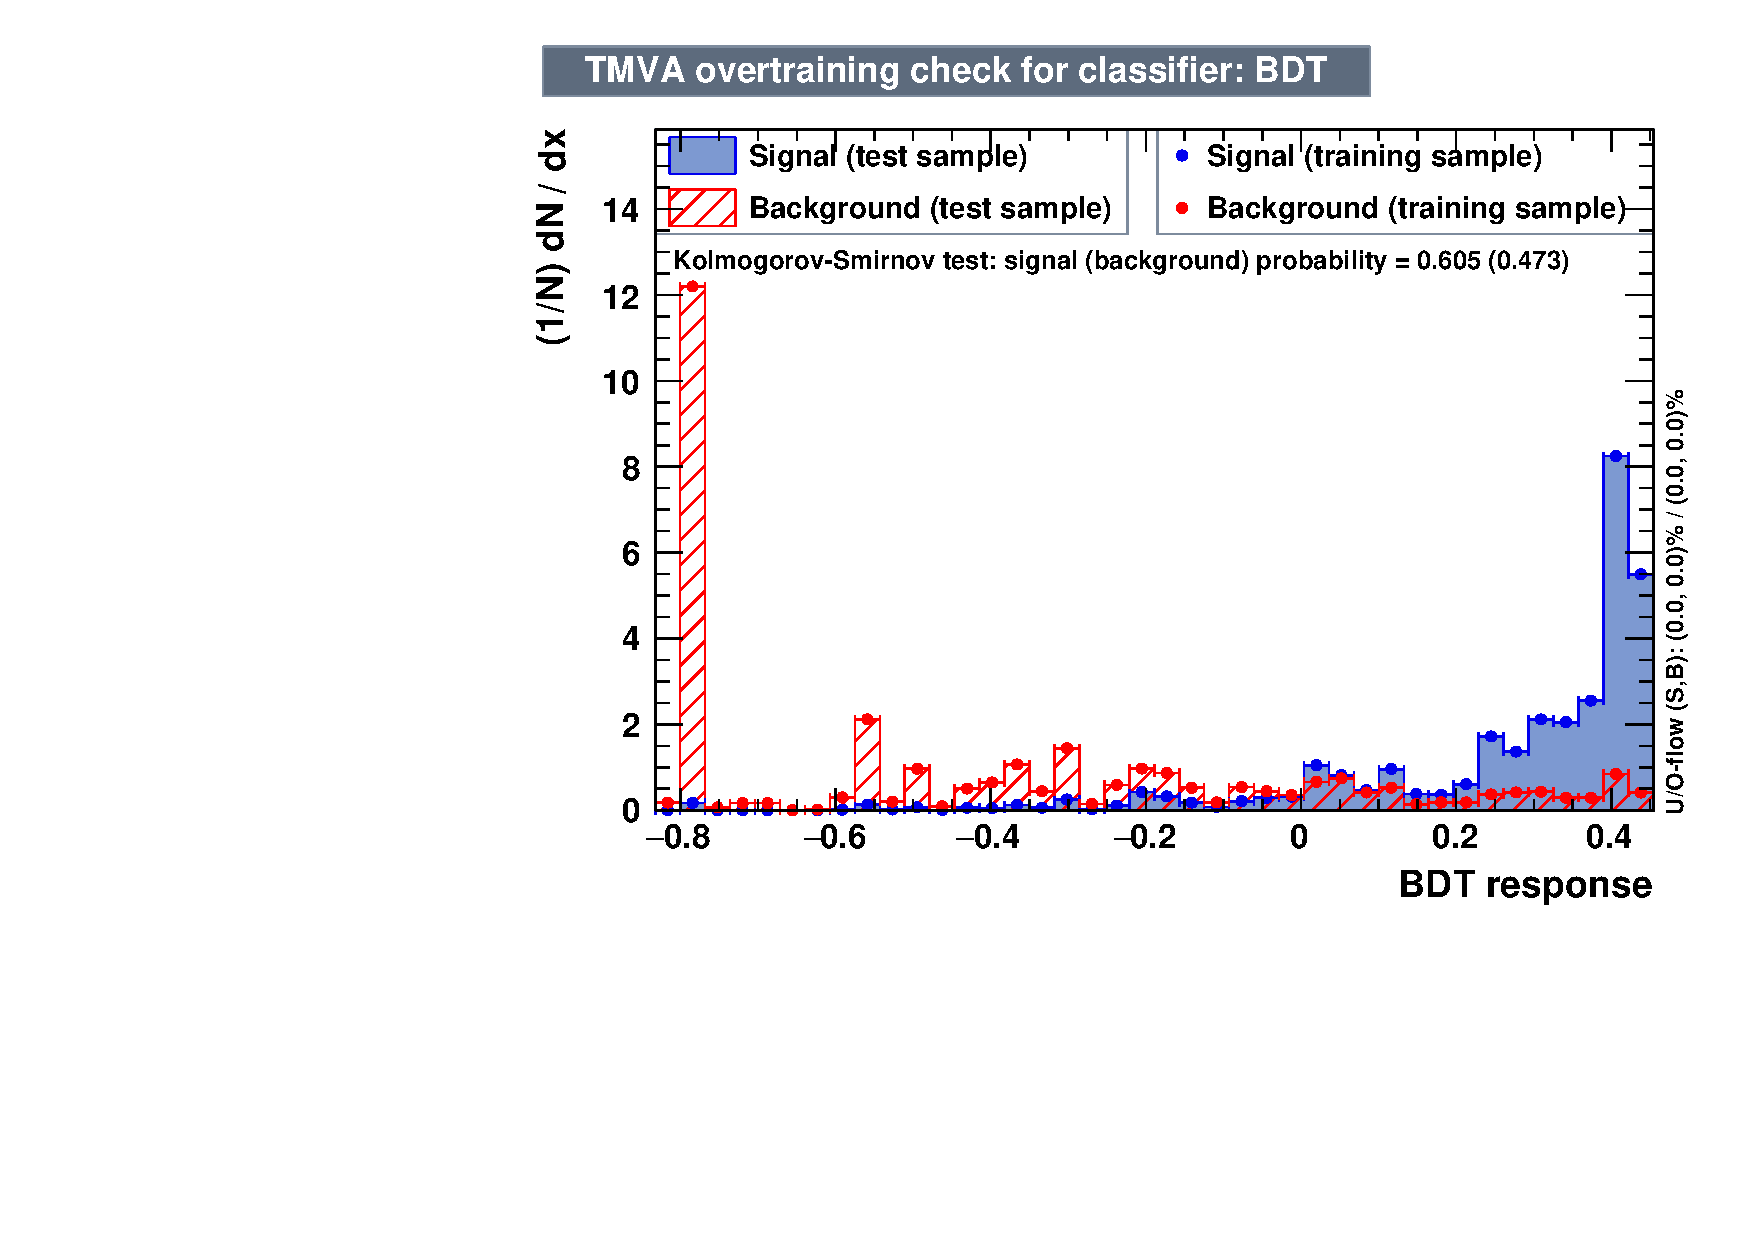
\includegraphics[width=0.45\textwidth]{Figures/EventSelReco/mva/a04_all_BDT_sep.pdf}}
			    \subfigure[BDTG's separation result]{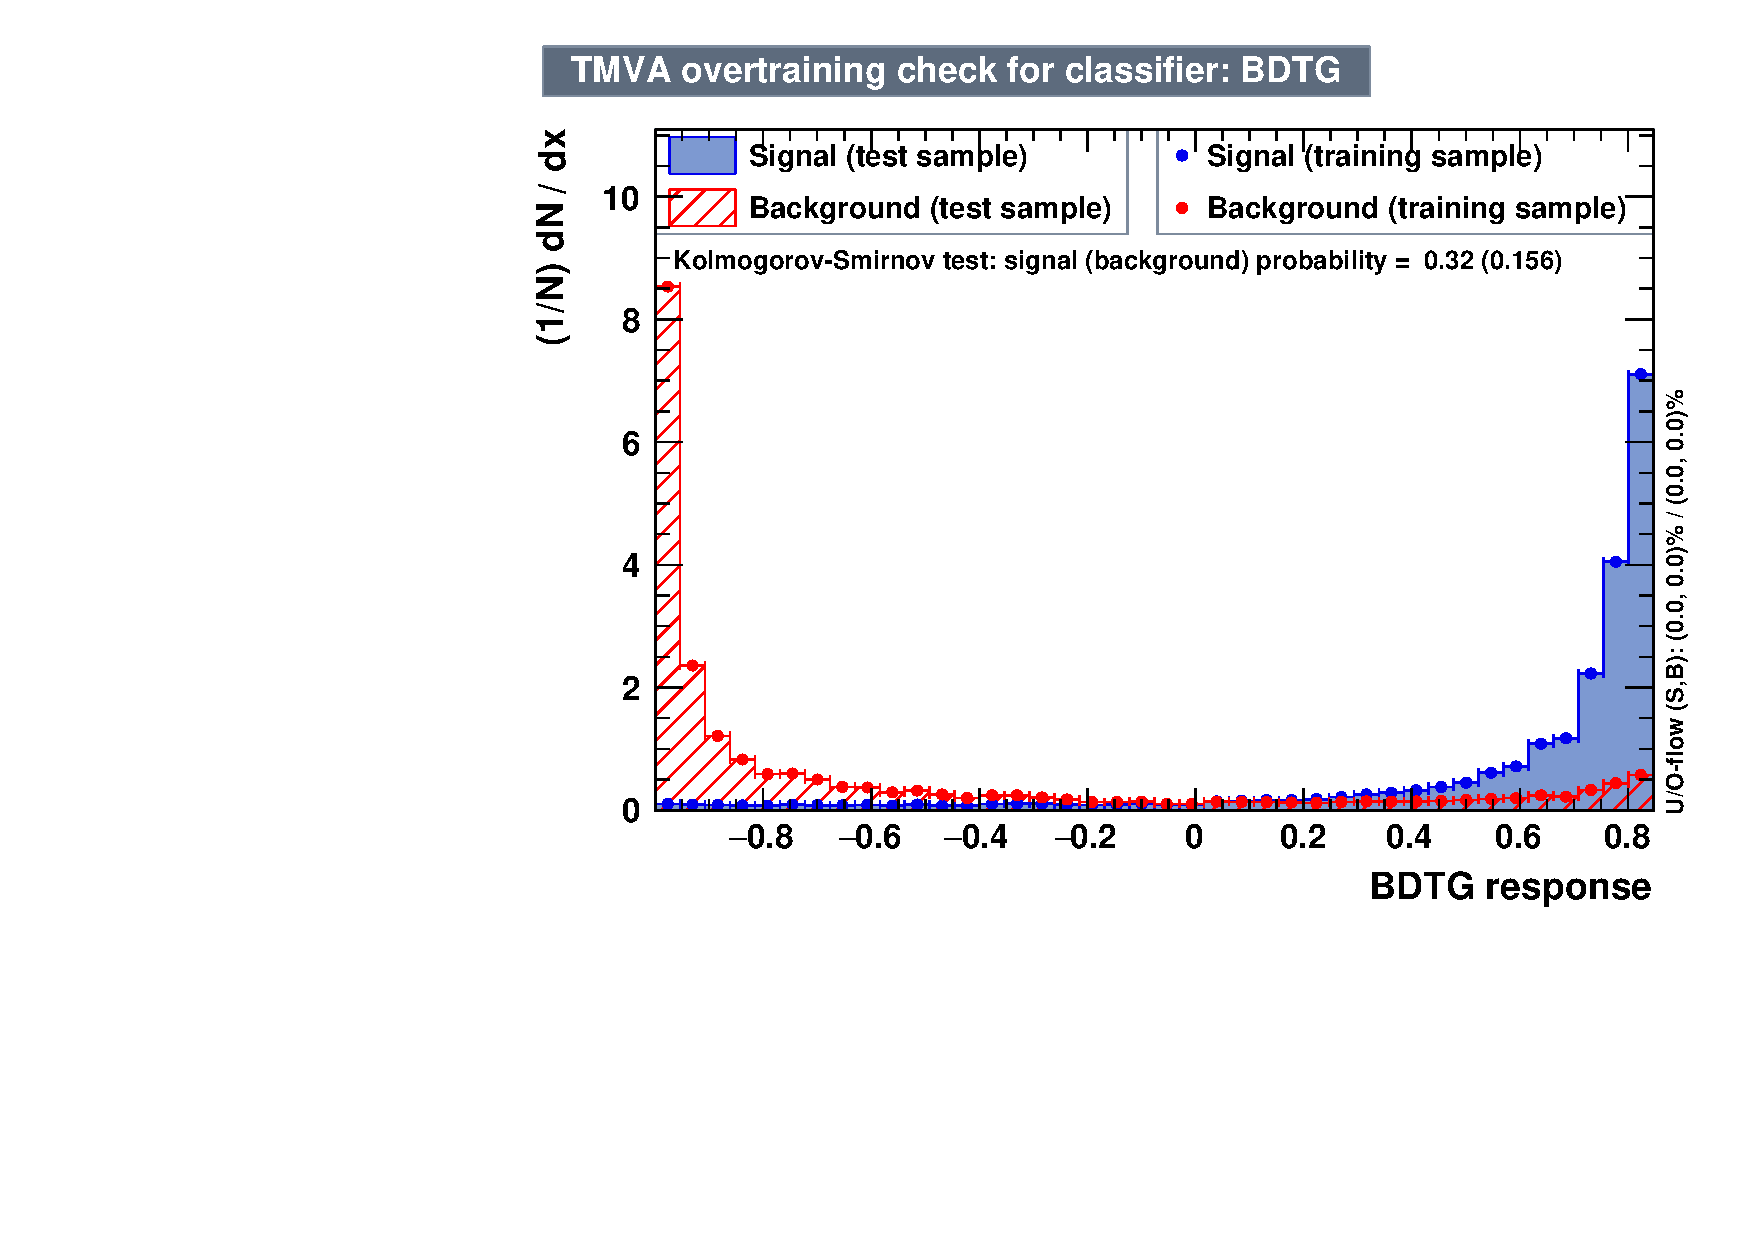
\includegraphics[width=0.45\textwidth]{Figures/EventSelReco/mva/a04_all_BDTG_sep.pdf}}\\
			    \subfigure[MLP's separation result]{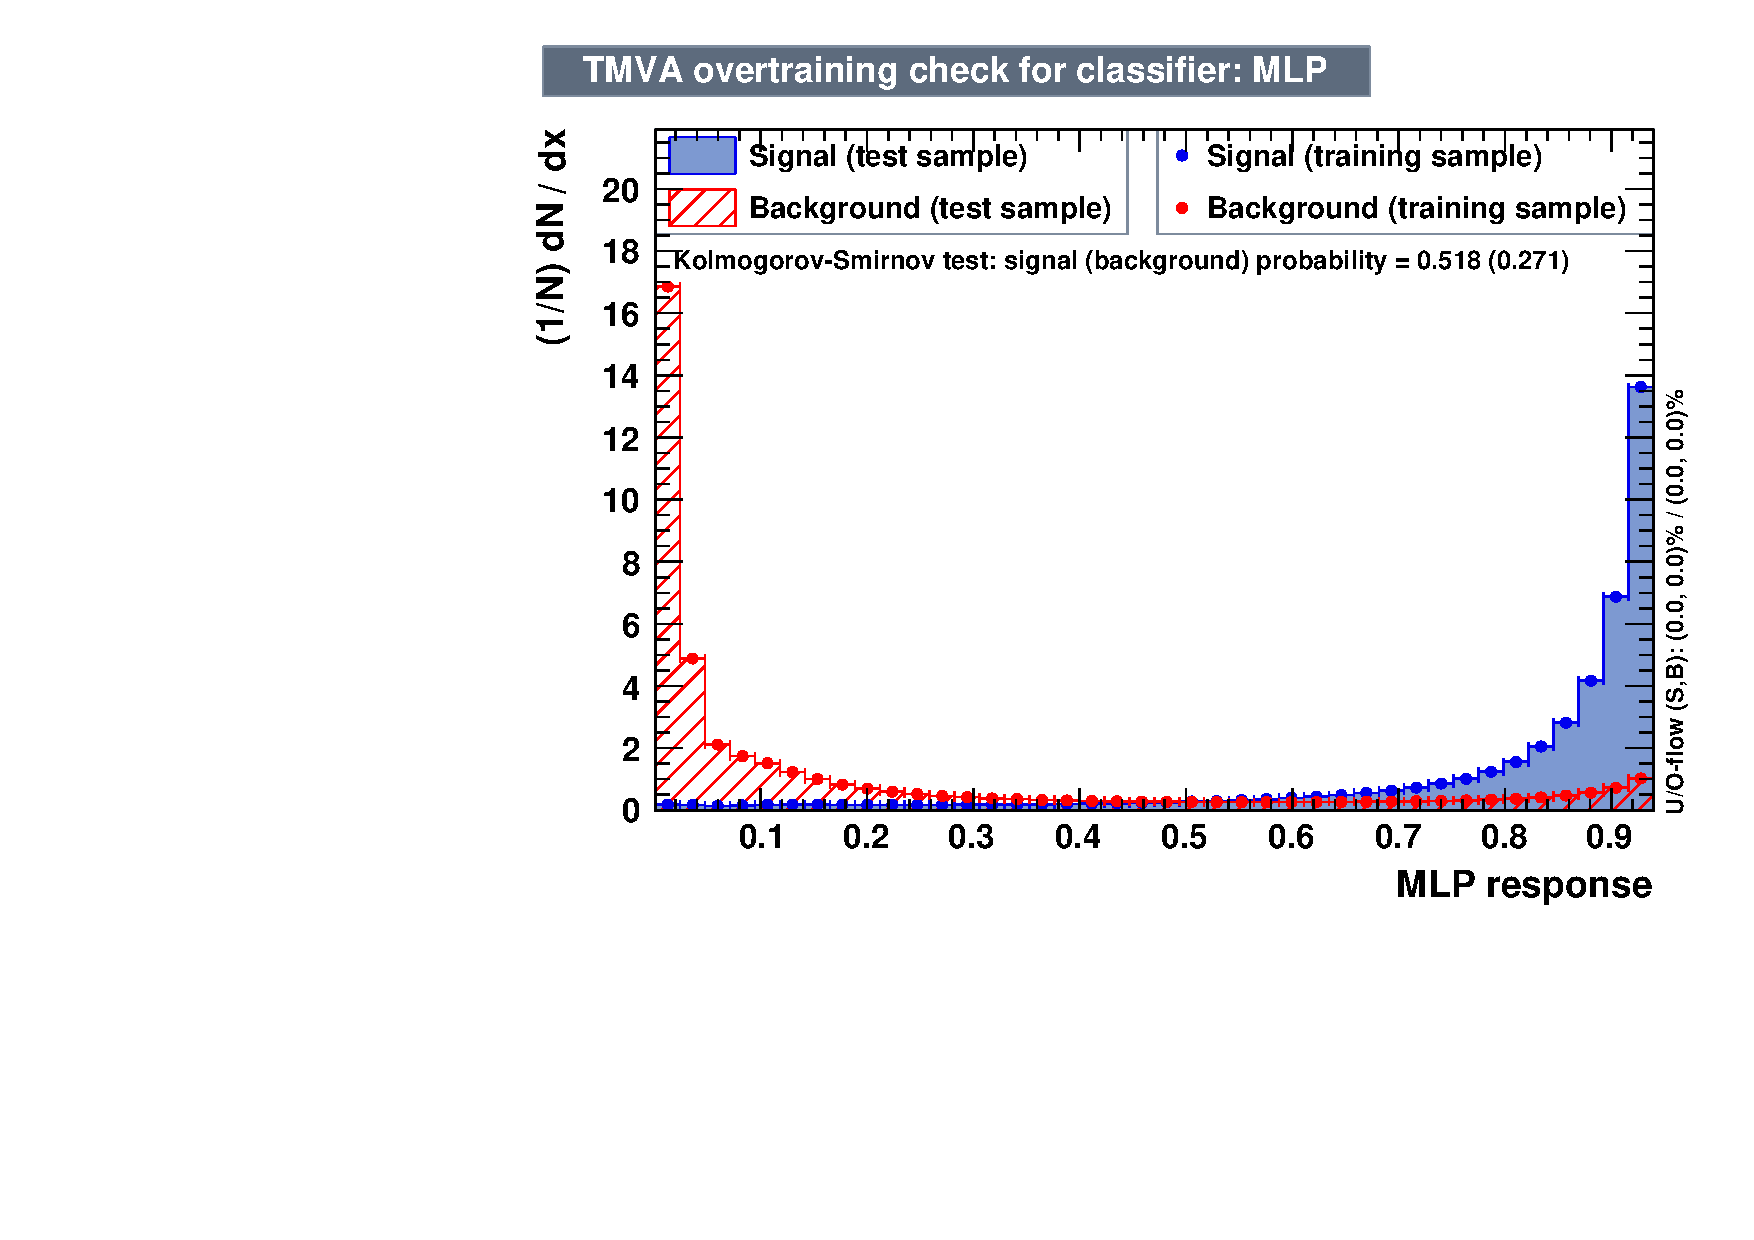
\includegraphics[width=0.45\textwidth]{Figures/EventSelReco/mva/a04_all_MLP_sep.pdf}}\\
			\caption{The seperating distribution on signal and background}
			\label{EventSelReco:fig:Sep_a04}
			\end{figure}
			\FloatBarrier

			The separation plots Fig.\ref{EventSelReco:fig:Sep_a04} shows the machine learning methods' separating ability through the input training variables. The distributions in these plots are the final separation performance between $"$signal$"$ and $"$background$"$(right and wrong objects combination) with the training values which is propagated from separations of all input variables(Fig.\ref{EventSelReco:fig:a04_varsep}). It is also the separation performance under training sample and testing sample with given machine learning method. As we can see that if we want to pick out $"$signal$"$(right combination), just choose the jjb combination who has the $\emph{highist MVA score}$ as the right one.

			\begin{figure}[H]
			\centering{}
			    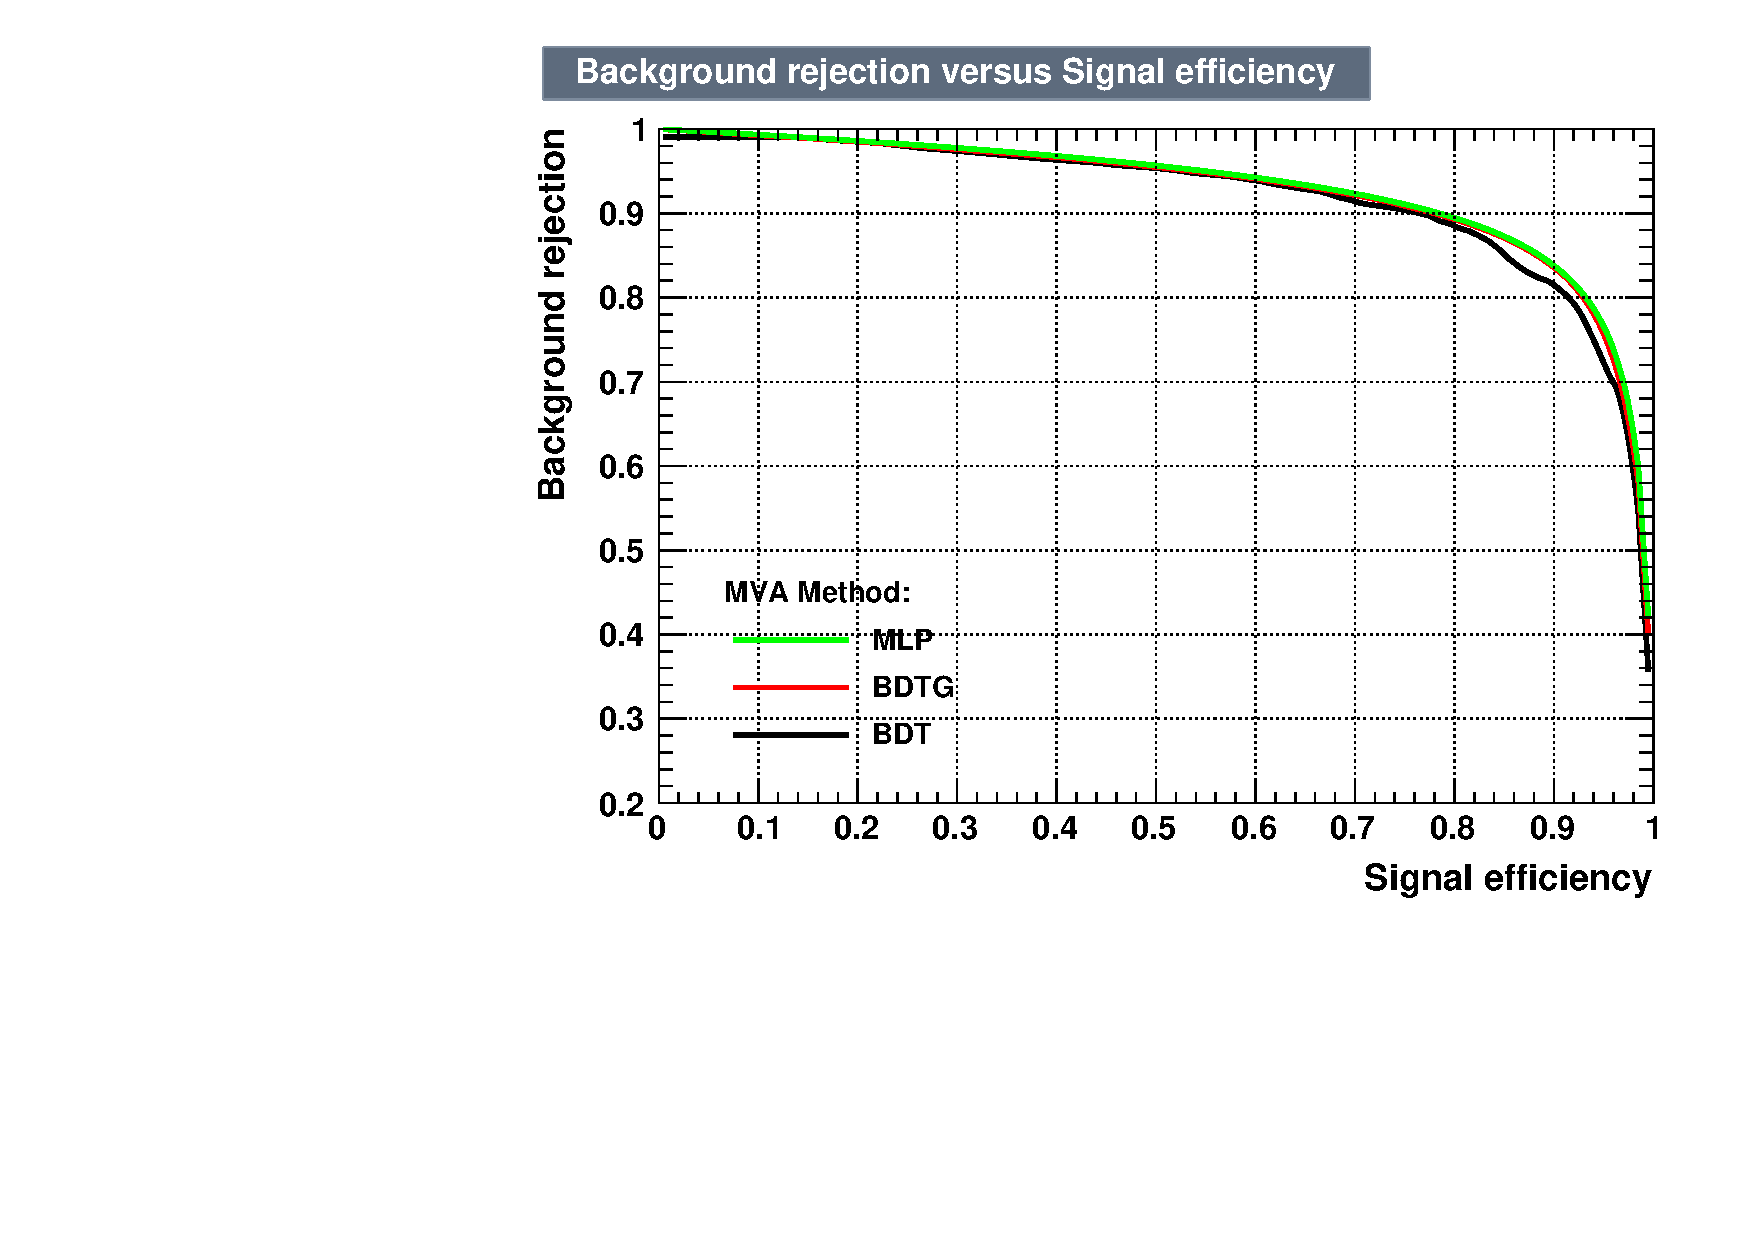
\includegraphics[width=0.6\textwidth]{Figures/EventSelReco/mva/a04_all_ROC.pdf}\\
			\caption{Receiver Operating Characteristic(ROC) curve of various machine learning method}
			\label{EventSelReco:fig:ROC_a04}
			\end{figure}
			\FloatBarrier
	
			The $\textbf{Receiver Operating Characteristic(ROC)}$ curve plot Fig.\ref{EventSelReco:fig:ROC_a04} can tell if it's given a cut on the output MVA score in separation distribution Fig.\ref{EventSelReco:fig:Sep_a04} to extract the $"$signal$"$, how the background rejection ratio vary when signal efficiency change. It can be infered that, the good performance is that when one rejects more ratio of background and at the same time reserves more ratio of signal(high signal efficiency). In other words, the bigger area under the ROC curve, the better the method is. However, the previous ROC criterion are just available and meaningful for the common case - one use MVA to separate the 2 different physics sample which are independent to each other, for example, use MVA to separate sigle $t$ and $t\bar{t}$ sample. In this analysis case, the signal and background are not separate like that kind in common. Being not independent 2 samples, signal and background are at the same time in one event instead. There are couple of complicated correlation between them. Therefore, the separation and ROC plots are not really fair anymore. As they going to not to be relative directly, there must be a standard to tell how MVA perform(That is the $b\bar{b}$ separation in \ref{ssec:bbsep}).

			There are also the reconstructed $M_{jjb}$ with MVA algorithm.($m_{jjb}$, $m_{jj}$) There is just MLP (instead of BDT/BDTG)results shown here.

			\begin{figure}[H]
			\centering
				\subfigure[muon channel]{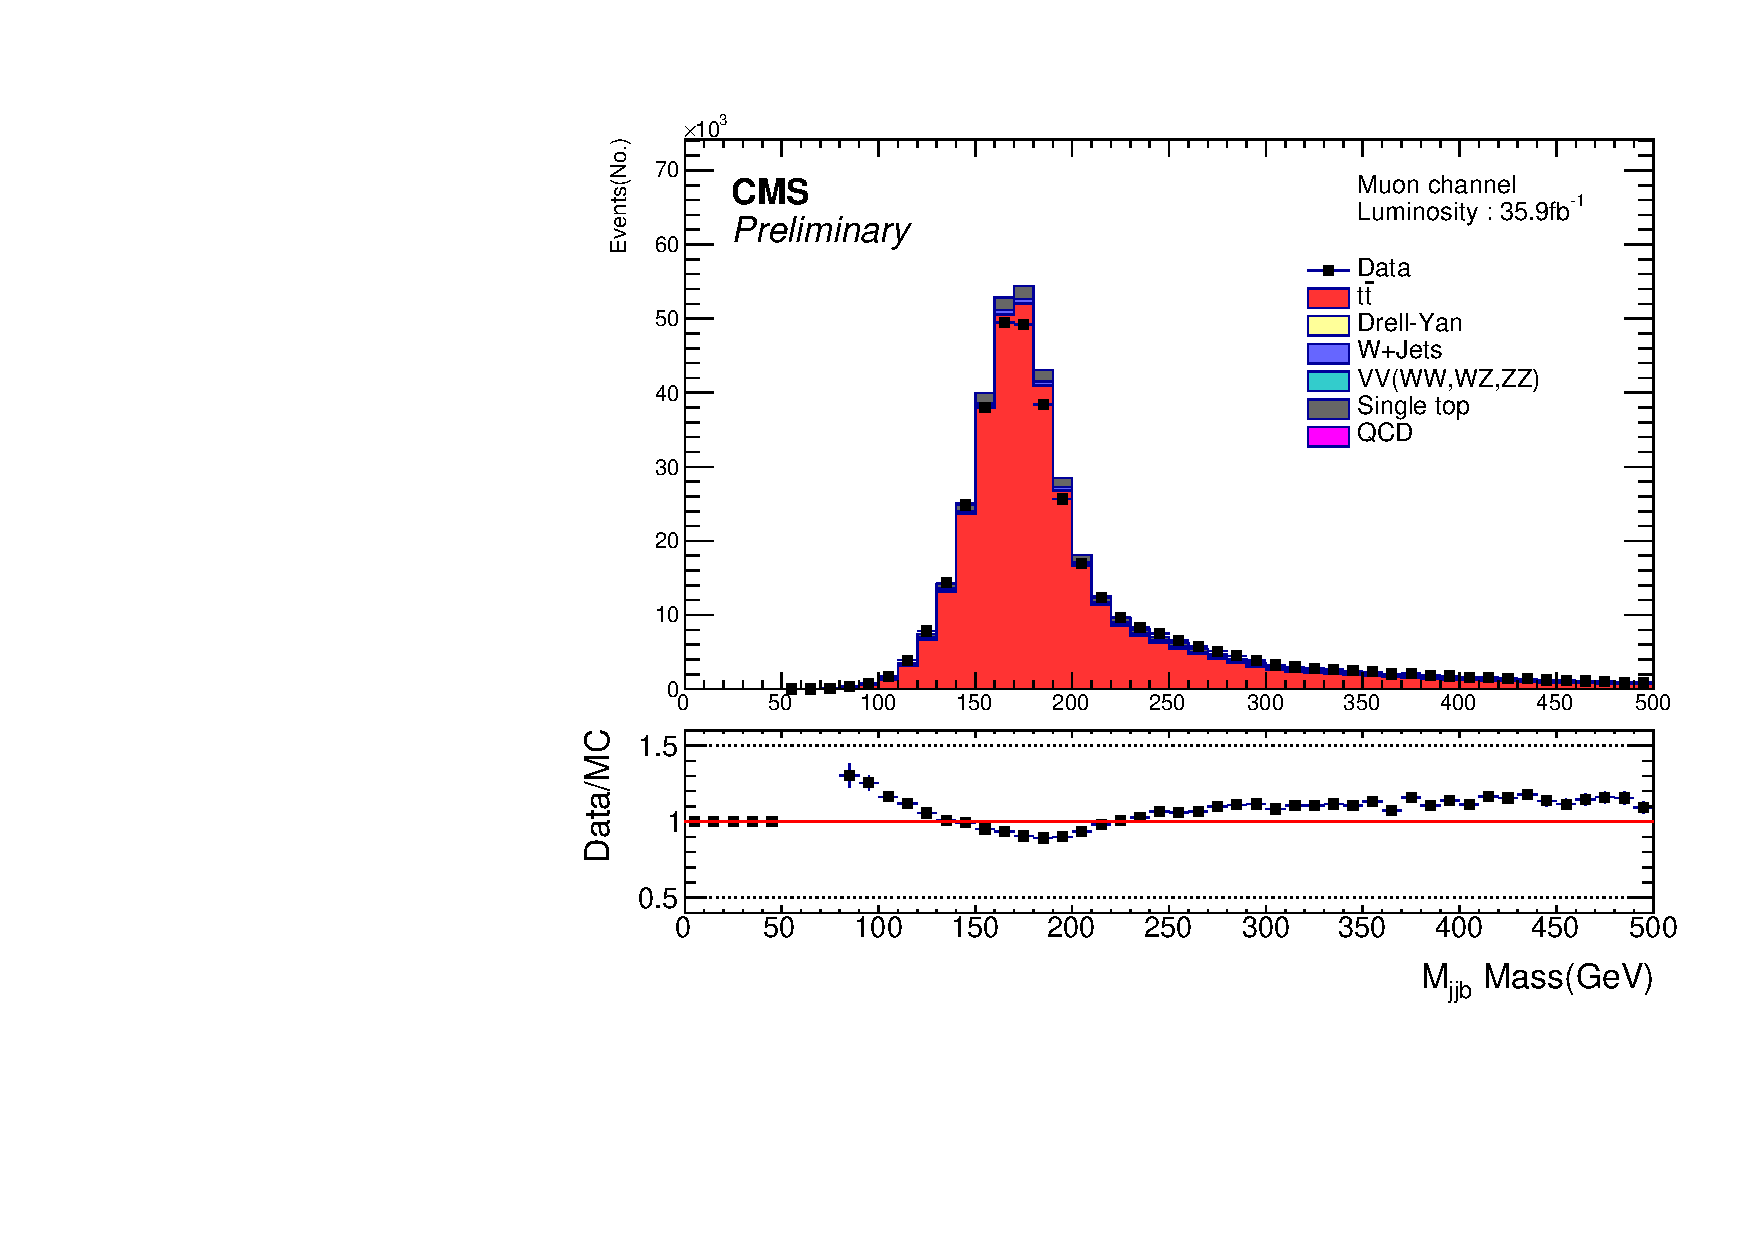
\includegraphics[width=0.45\textwidth]{Figures/EventSelReco/Mass/a04/a04_MLP_NC_long_HadTop_mu.pdf}}
			    \subfigure[electron channel]{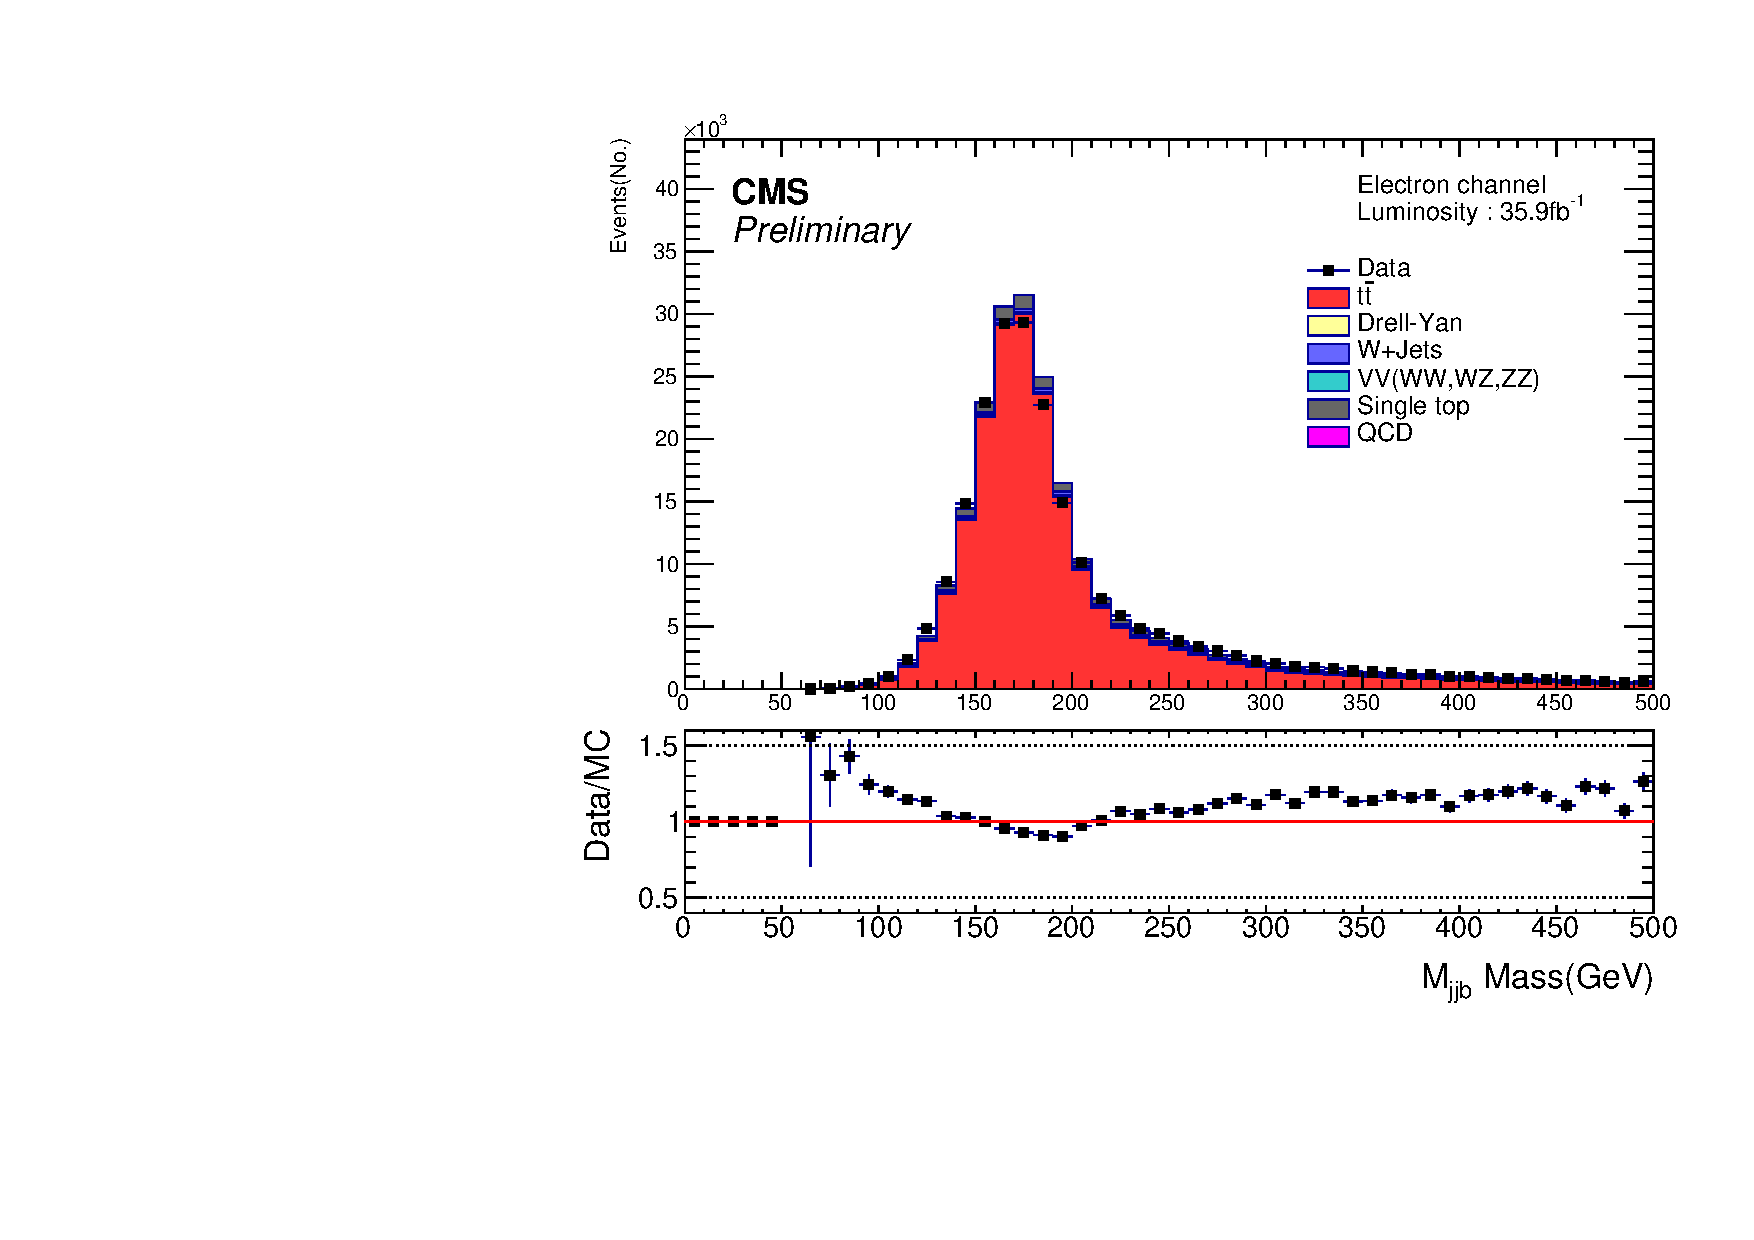
\includegraphics[width=0.45\textwidth]{Figures/EventSelReco/Mass/a04/a04_MLP_NC_long_HadTop_el.pdf}}\\
			\caption{Reconstructed $M_{jjb}$ with 2 variables MLP algorithm (w/o cut)}
			\label{EventSelReco:fig:a04_MLP_SR_NC_Mjjb}
			\end{figure}
			\FloatBarrier

			And also, it is better to use MVA with more variables than just $m_{jj}$ and $m_{jjb}$. There are 3 variables sets after a bunch of trials here to input and train. It's a remindful item that they are the variables of each combination in any event.

			\begin{enumerate}
			\item The first set: (2 variables)
				\begin{itemize}
				\item $m_{jjb}$, $m_{jj}$
				\end{itemize}

			%%% TODO: this set need to be eliminate before showing the result of bbsep performance
			\item The second set: (8 variables)
				\begin{itemize}
				\item $m_{jjb}$, $m_{jj}$
				\item 2 jets'(jj) $\emph{sum of}$ $P_{T}$, $\Delta \phi$, $\Delta \eta$
				\item selected lepton and leptonic b-jet's $\emph{sum of}$ $P_{T}$, $\Delta \phi$, $\Delta \eta$ 
				\end{itemize}

			\item The third set: (20 variables)
				\begin{itemize}
				\item $m_{jjb}$, $m_{jj}$
				\item 2 jets'(jj) $\emph{sum of}$ $P_{T}$, $|\Delta P_{T}|$, $\Delta R$
				\item hadronic W(j+j) and hadronic b-jet's $\emph{sum of}$ $P_{T}$, $|\Delta P_{T}|$, $\Delta R$
				\item selected lepton and hadronic b-jet's $\emph{sum of}$ $P_{T}$, $|\Delta P_{T}|$, $\Delta R$
				\item selected lepton and hadronic W(j+j)'s $\emph{sum of}$ $P_{T}$, $|\Delta P_{T}|$, $\Delta R$
				\item hadronic W(j+j) and MET's $\emph{sum of}$ $P_{T}$, $|\Delta P_{T}|$, $\Delta \phi$
				\item hadronic b-jet and MET's $\emph{sum of}$ $P_{T}$, $|\Delta P_{T}|$, $\Delta \phi$
				\end{itemize}
			\label{EventSelReco:itm:mva_var}
			\end{enumerate}

			Besides the training result of the 2 variables' set have been shown(Fig.\ref{EventSelReco:fig:a04_varsep}, Fig.\ref{EventSelReco:fig:Sep_a04}, Fig.\ref{EventSelReco:fig:ROC_a04}), there are also the training results of 8 variables and 20 variables' cases:

			\begin{figure}[H]
			\centering{}
    			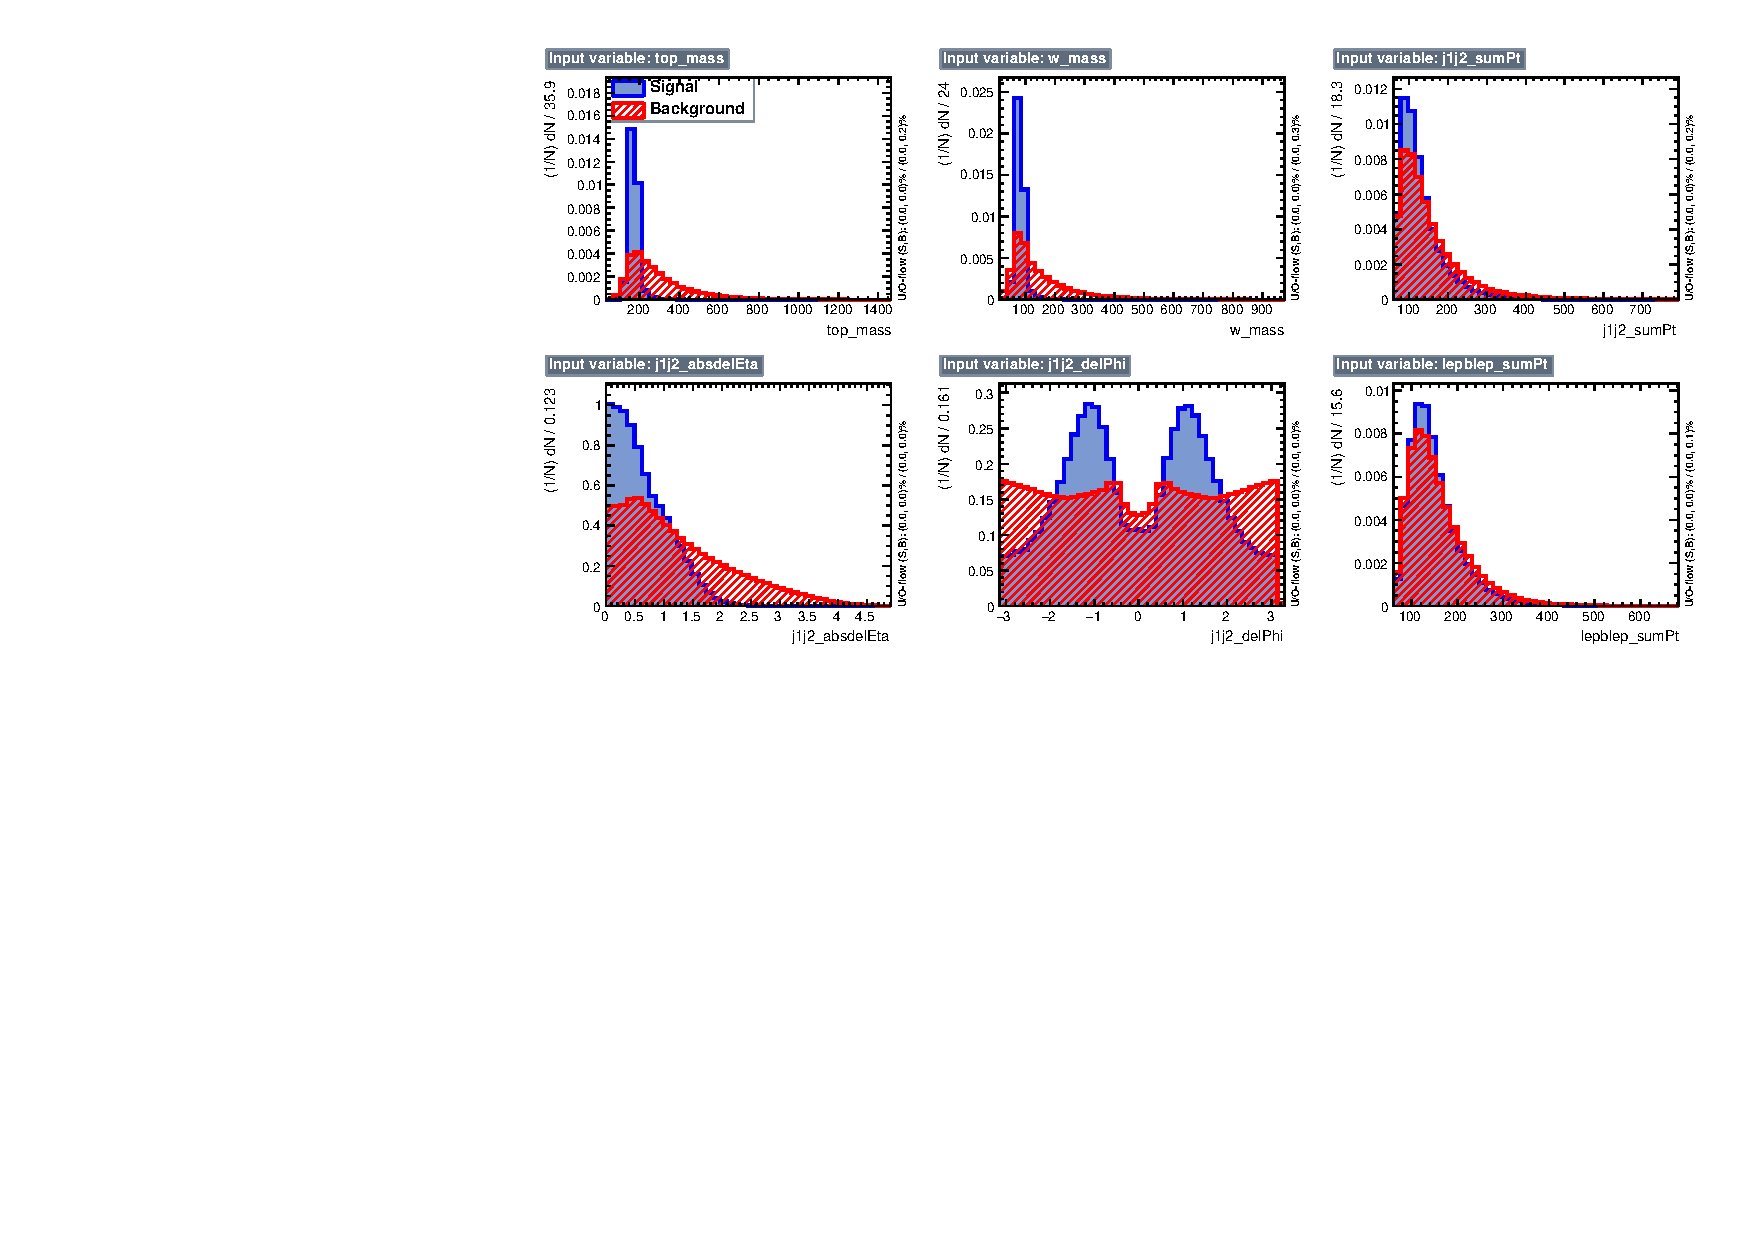
\includegraphics[width=0.8\textwidth]{Figures/EventSelReco/mva/t13_VarSep1.pdf}\\
			\end{figure}
			\FloatBarrier
			\begin{figure}[H]
			\centering{}
    			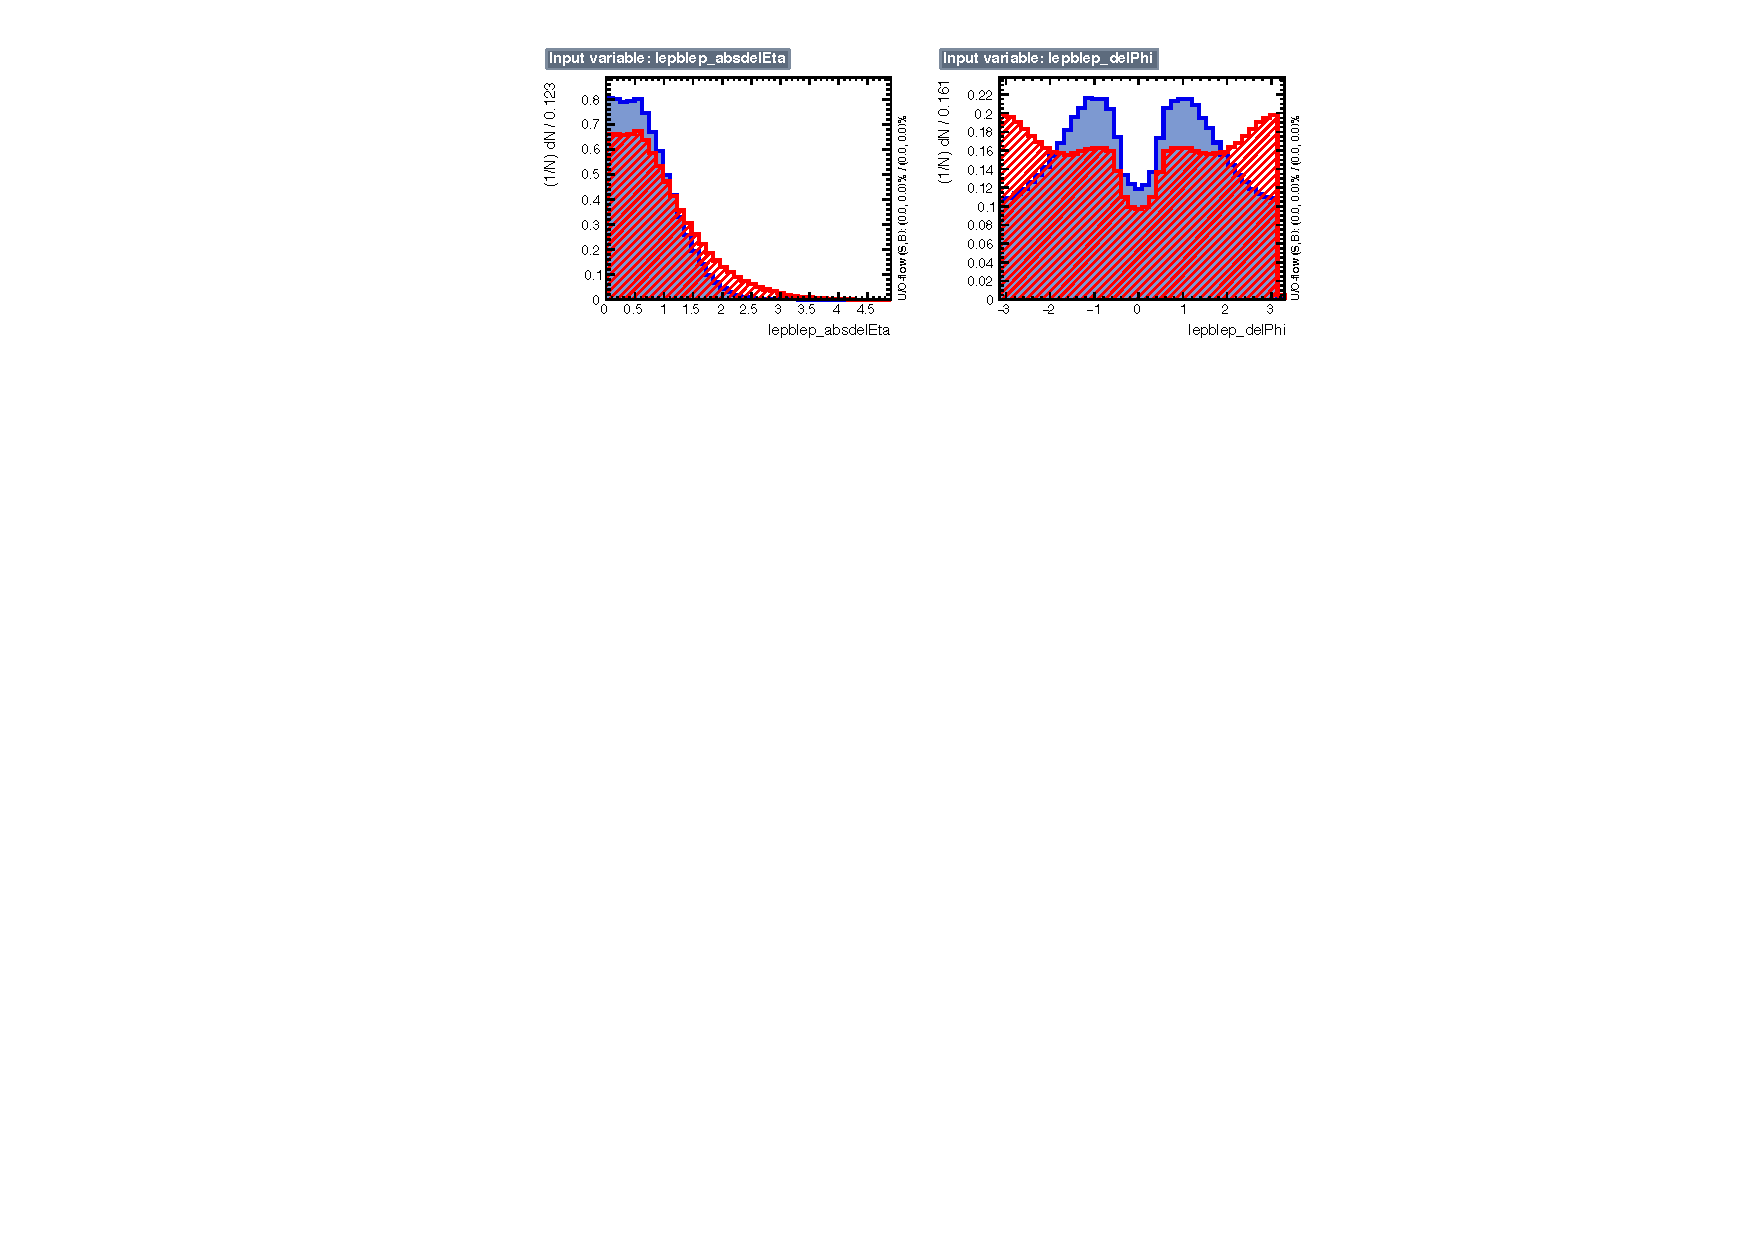
\includegraphics[width=0.528\textwidth]{Figures/EventSelReco/mva/t13_VarSep2.pdf}\\
    		\caption{Input training variables separation between $"$signal$"$ and $"$background$"$.(8 variables)}
			\label{EventSelReco:fig:t13_varsep}
			\end{figure}
			\FloatBarrier

			\begin{figure}[H]
			\centering
				\subfigure[BDT's separation result (8 vars)]{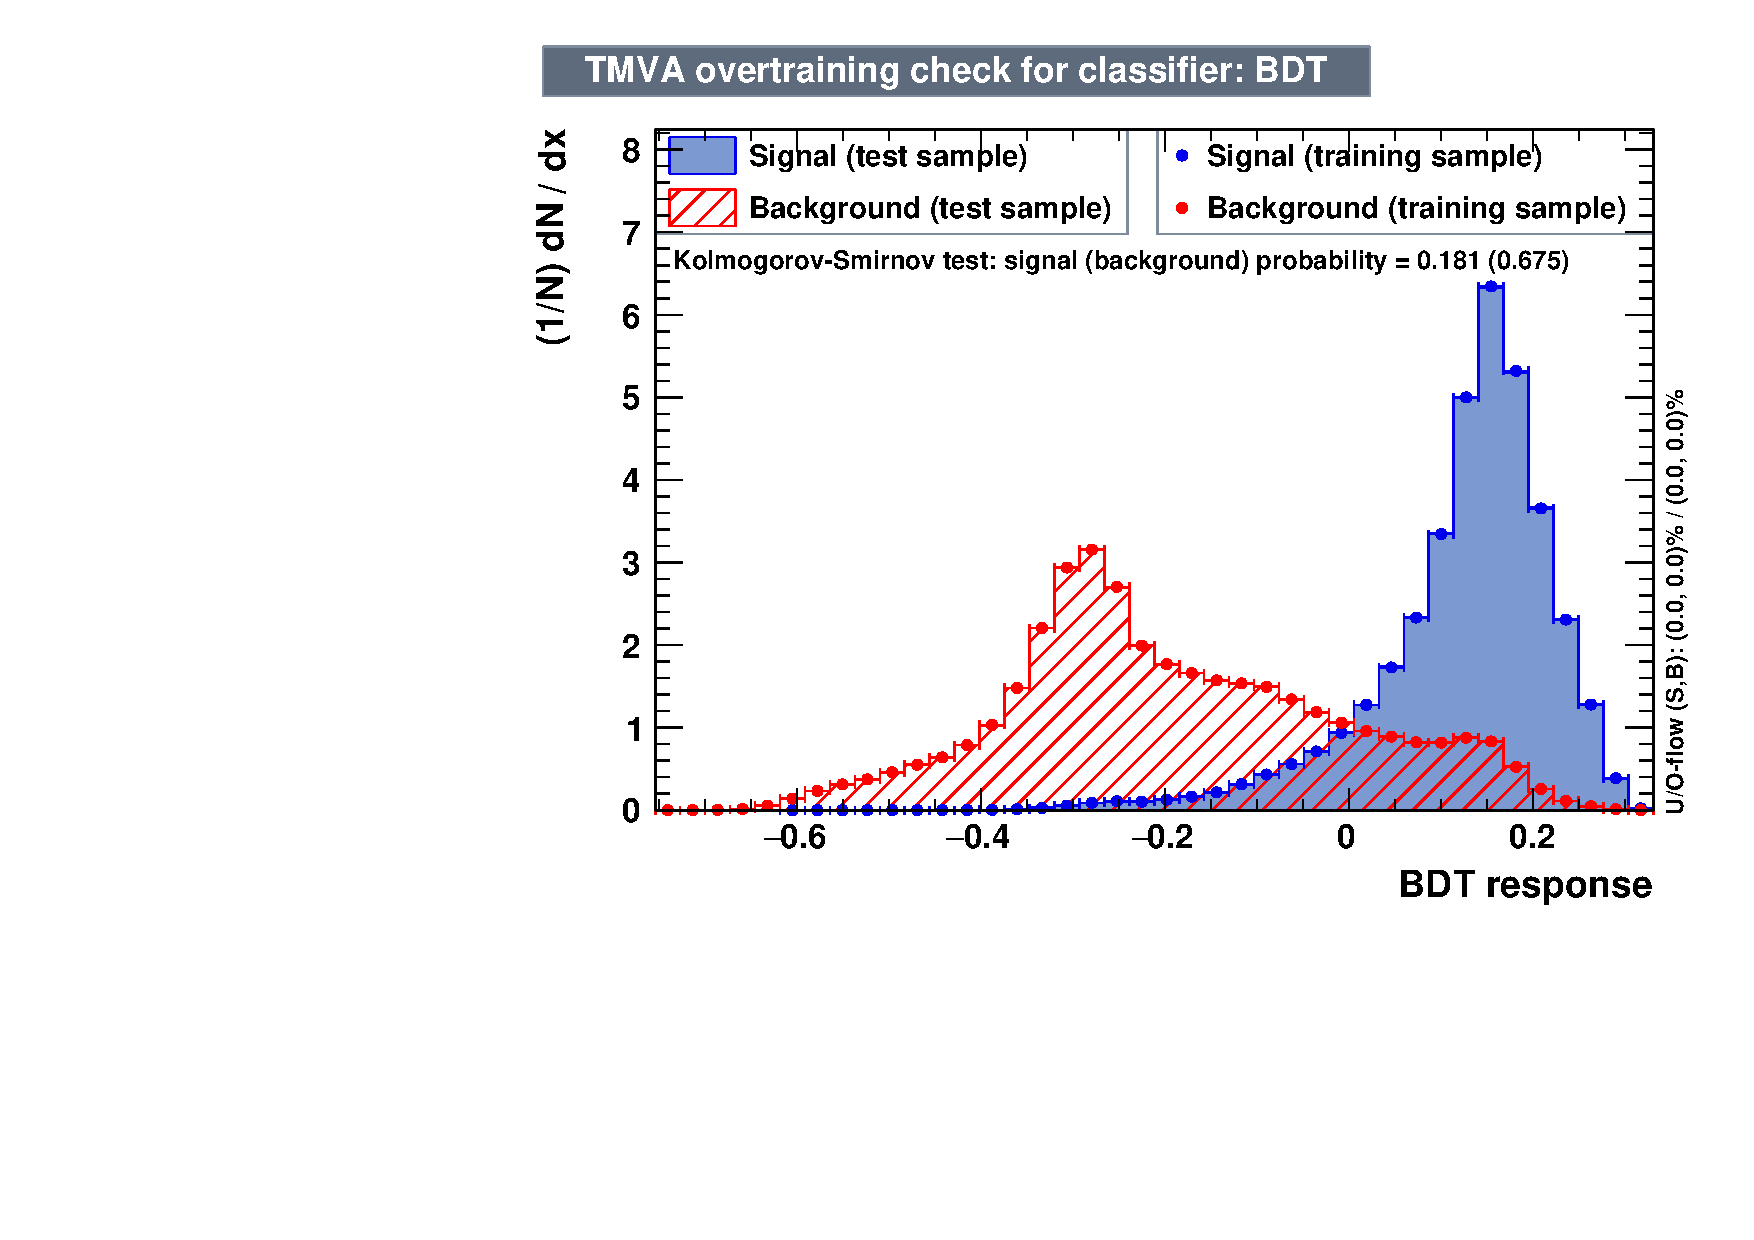
\includegraphics[width=0.4\textwidth]{Figures/EventSelReco/mva/t13_BDT_sep.pdf}}
			    \subfigure[BDTG's separation result (8 vars)]{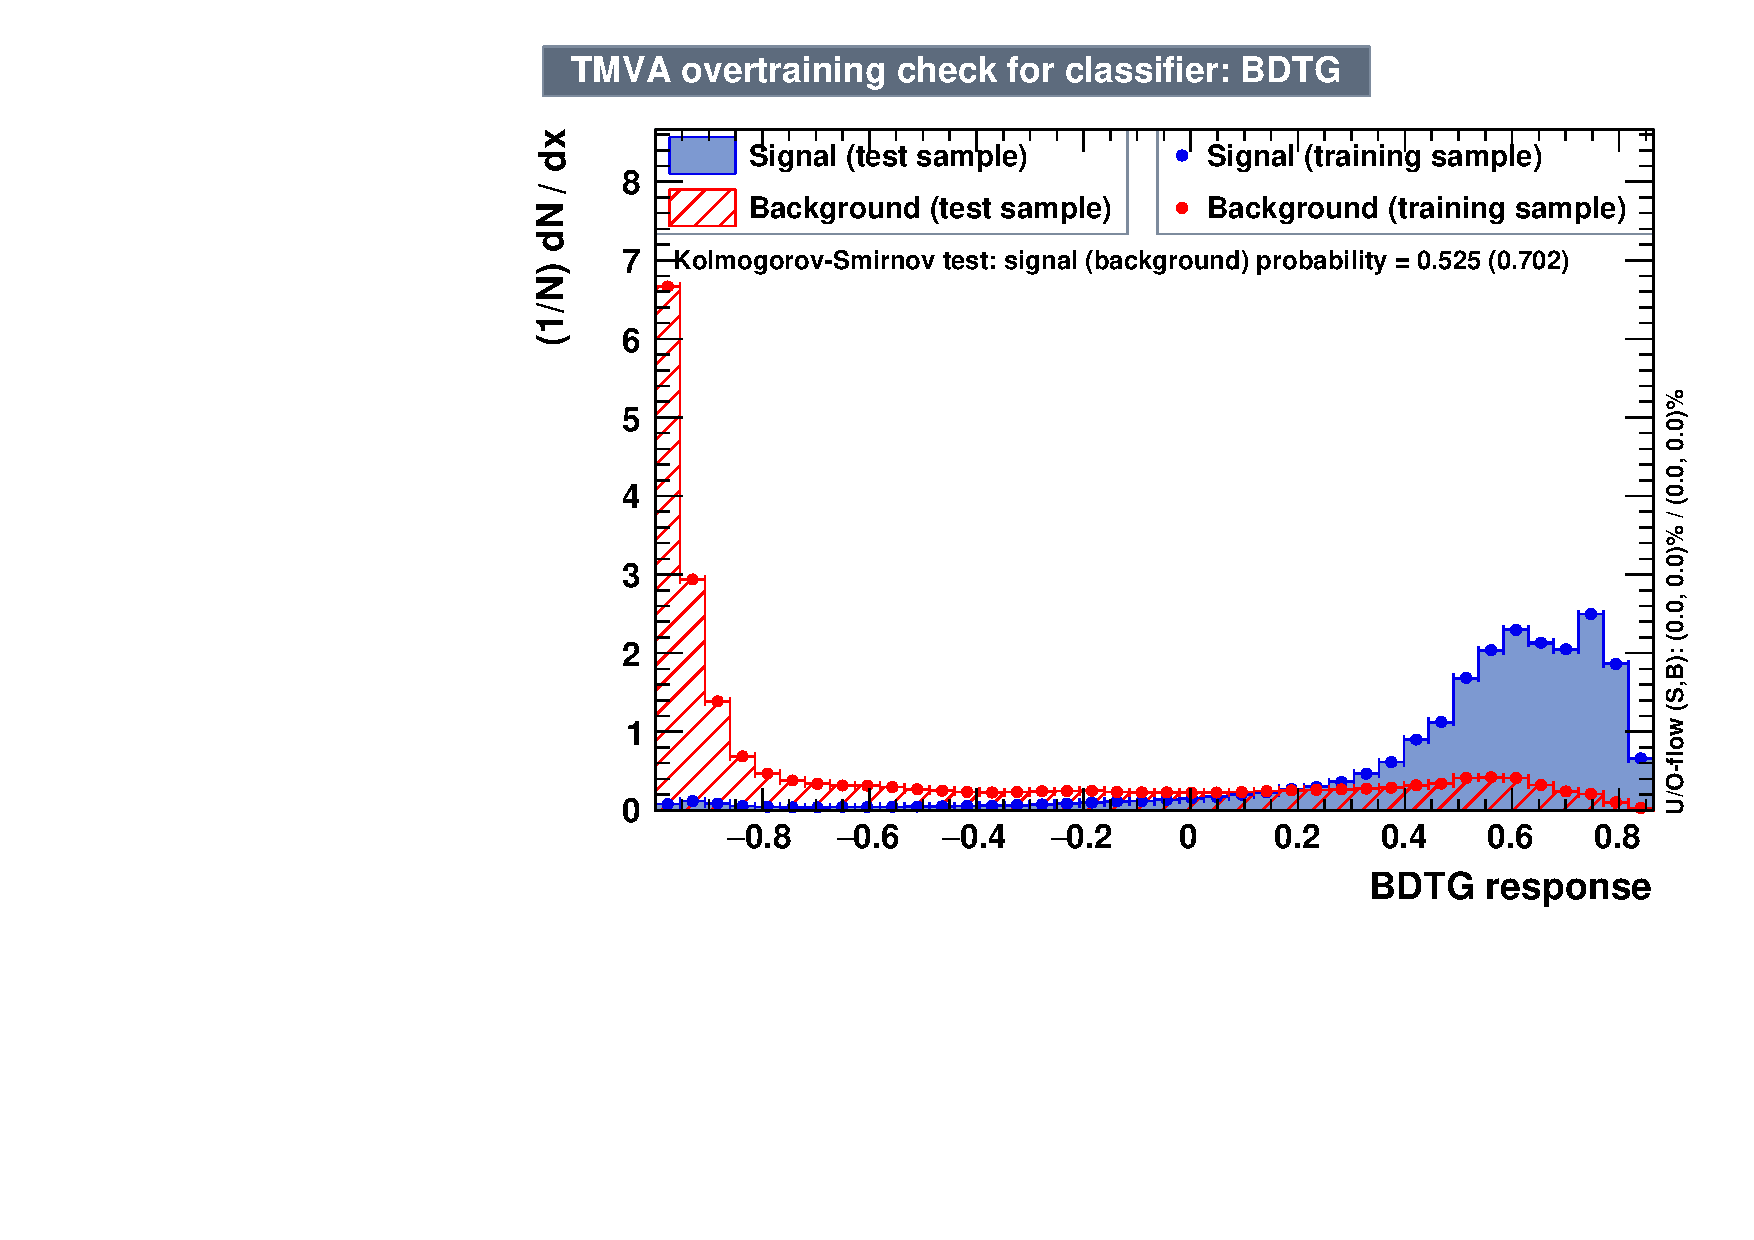
\includegraphics[width=0.4\textwidth]{Figures/EventSelReco/mva/t13_BDTG_sep.pdf}}\\
			\end{figure}
			\FloatBarrier
			\begin{figure}[H]
			\centering
			    \subfigure[MLP's separation result (8 vars)]{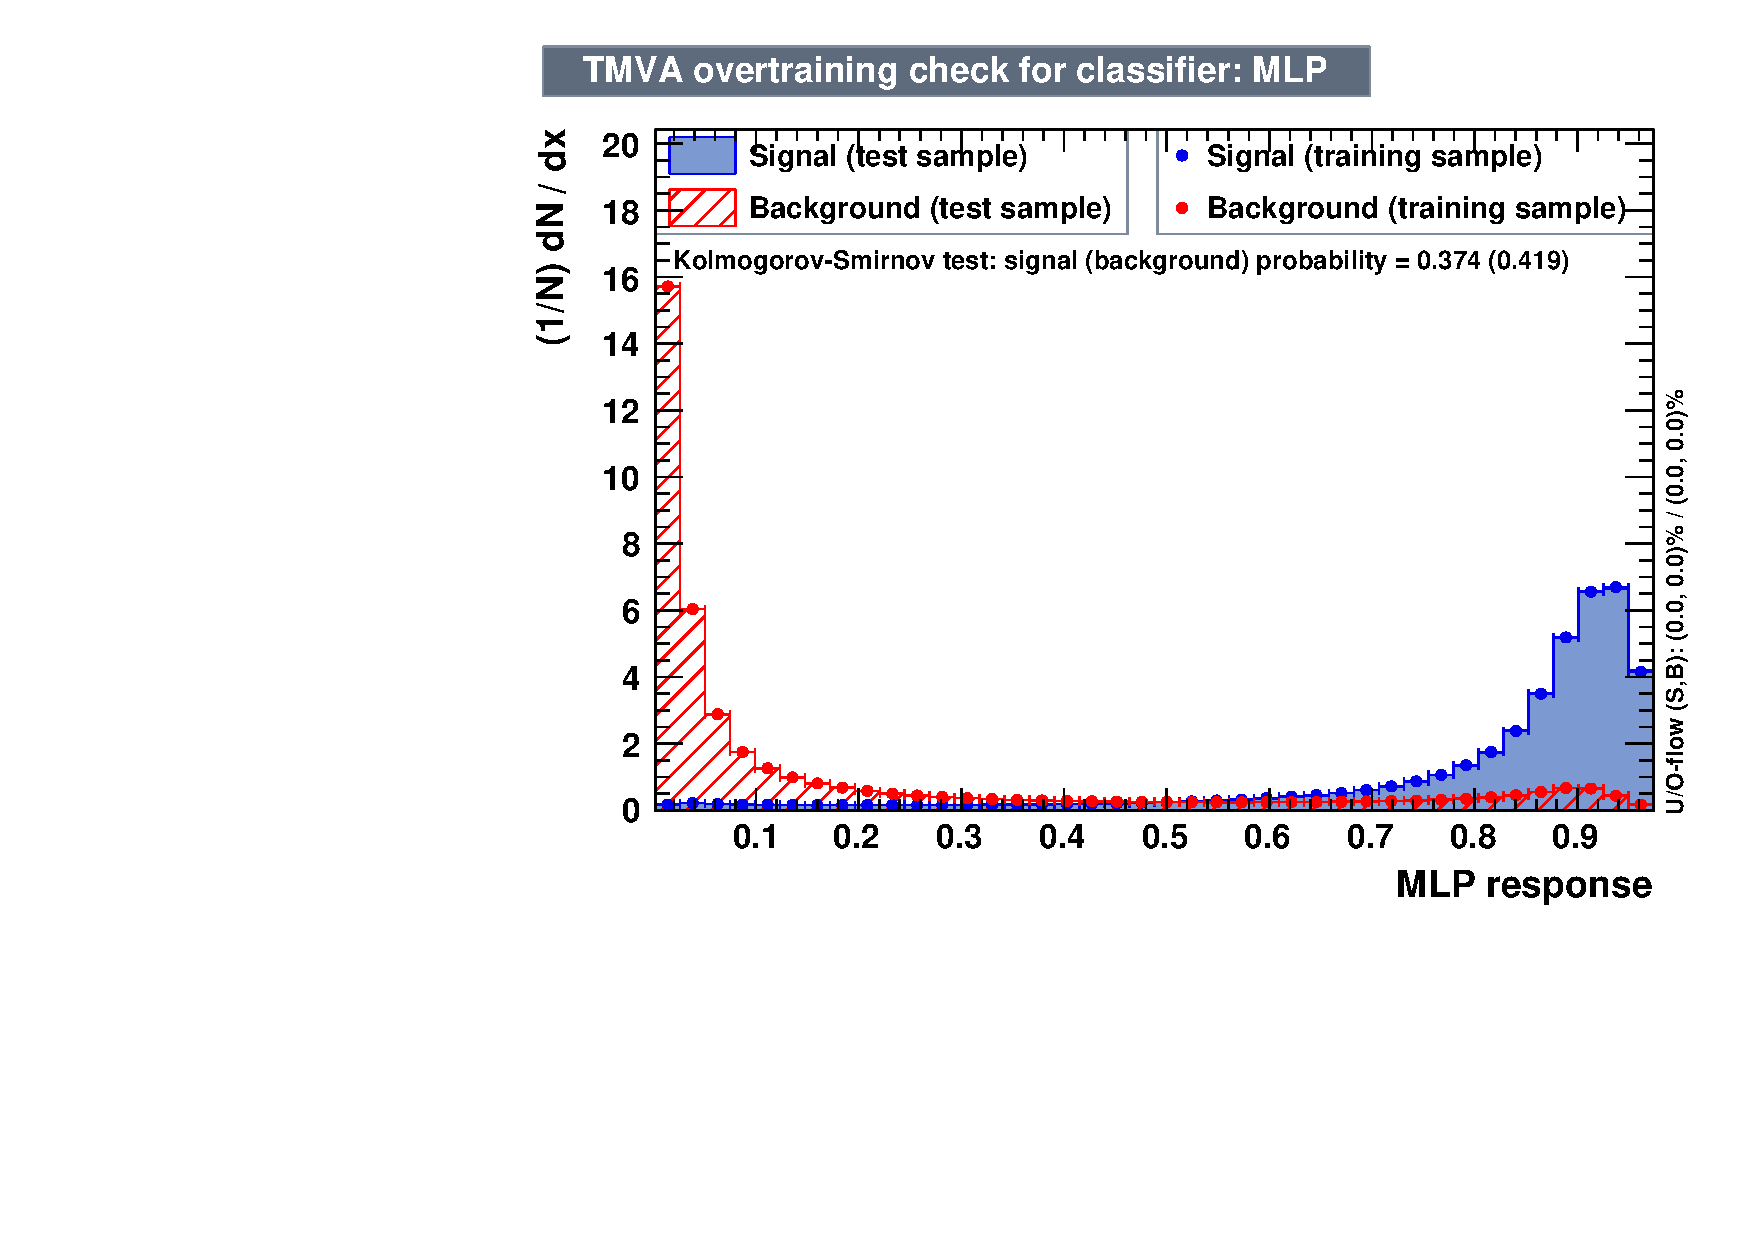
\includegraphics[width=0.4\textwidth]{Figures/EventSelReco/mva/t13_MLP_sep.pdf}}
			    \subfigure[ROC curve (8 vars)]{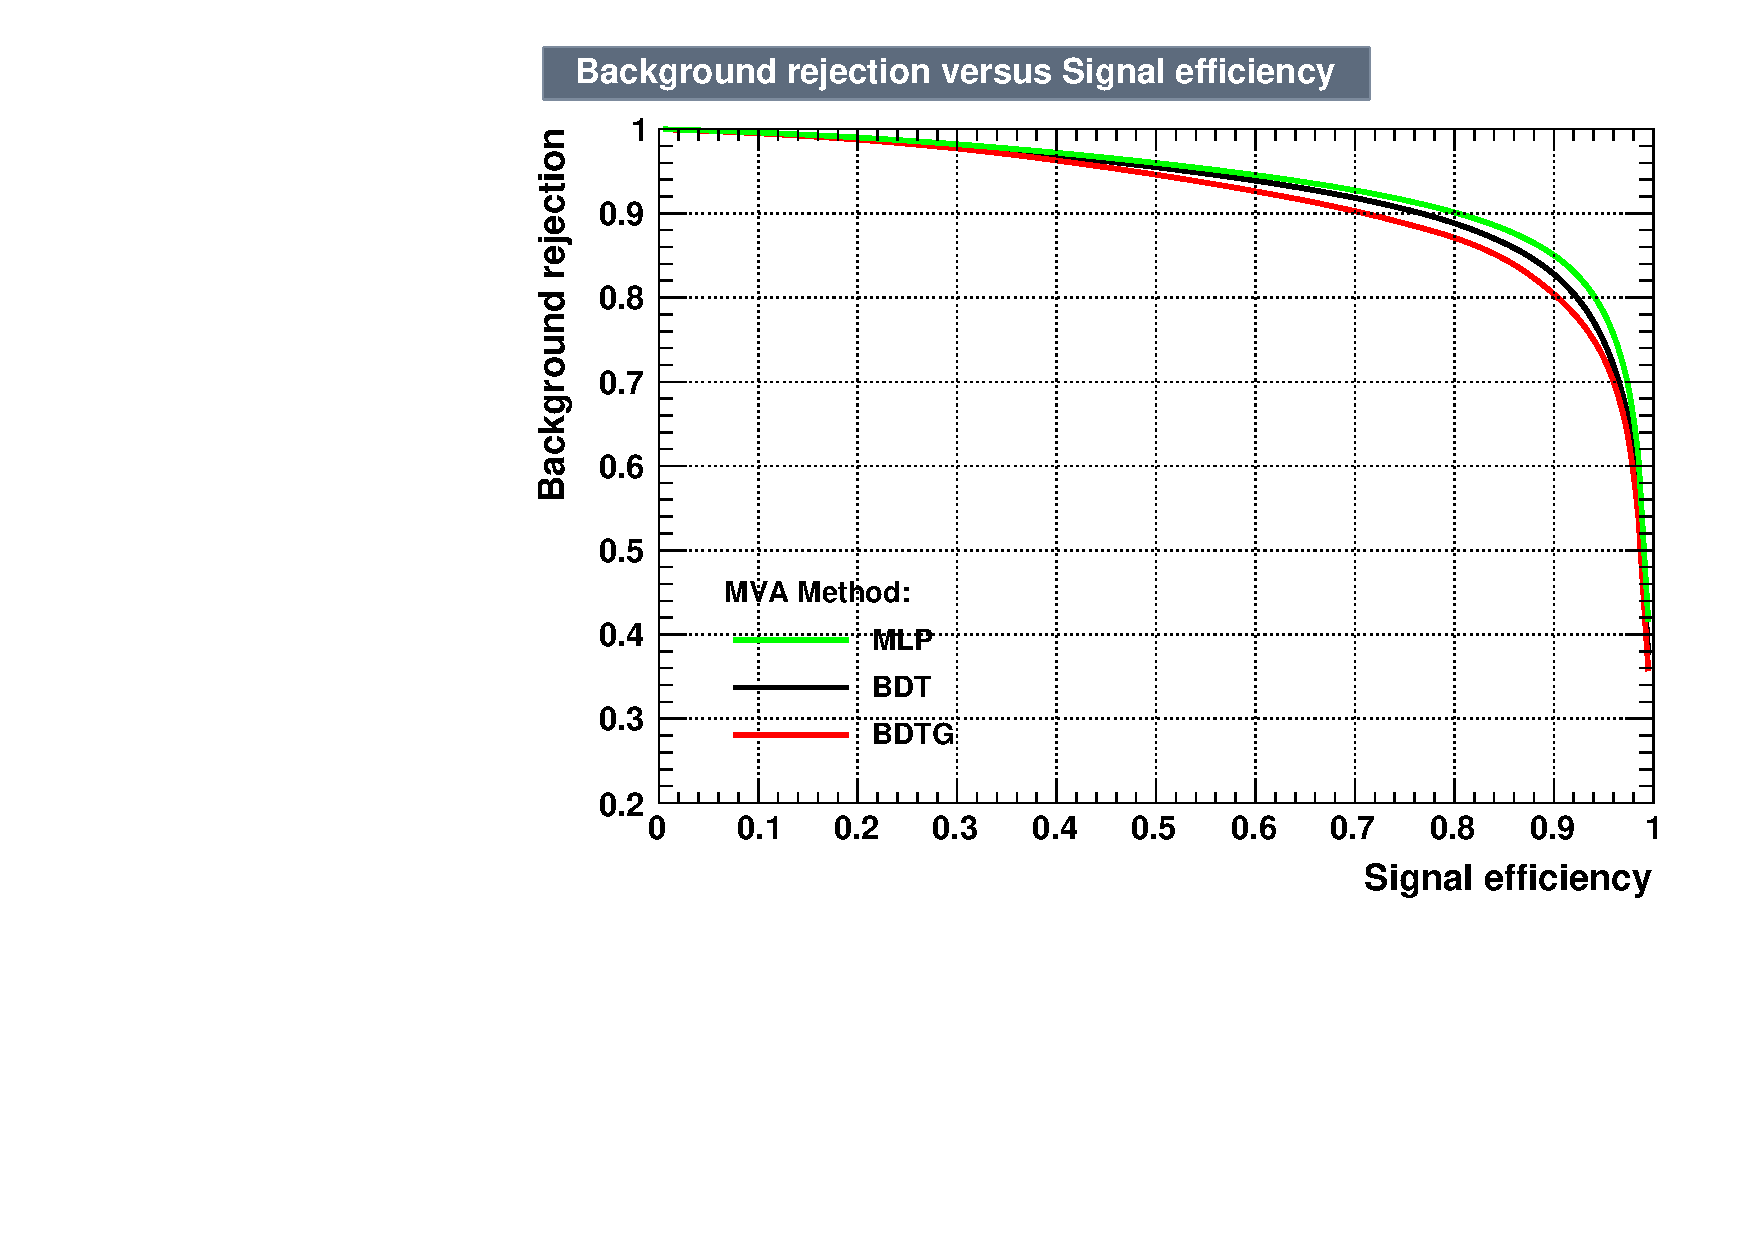
\includegraphics[width=0.4\textwidth]{Figures/EventSelReco/mva/t13_ROC.pdf}}\\
			\caption{The training result of 8 variables set}
			\label{EventSelReco:fig:Sep_ROC_t13}
			\end{figure}
			\FloatBarrier

			\begin{figure}[H]
			\centering{}
    			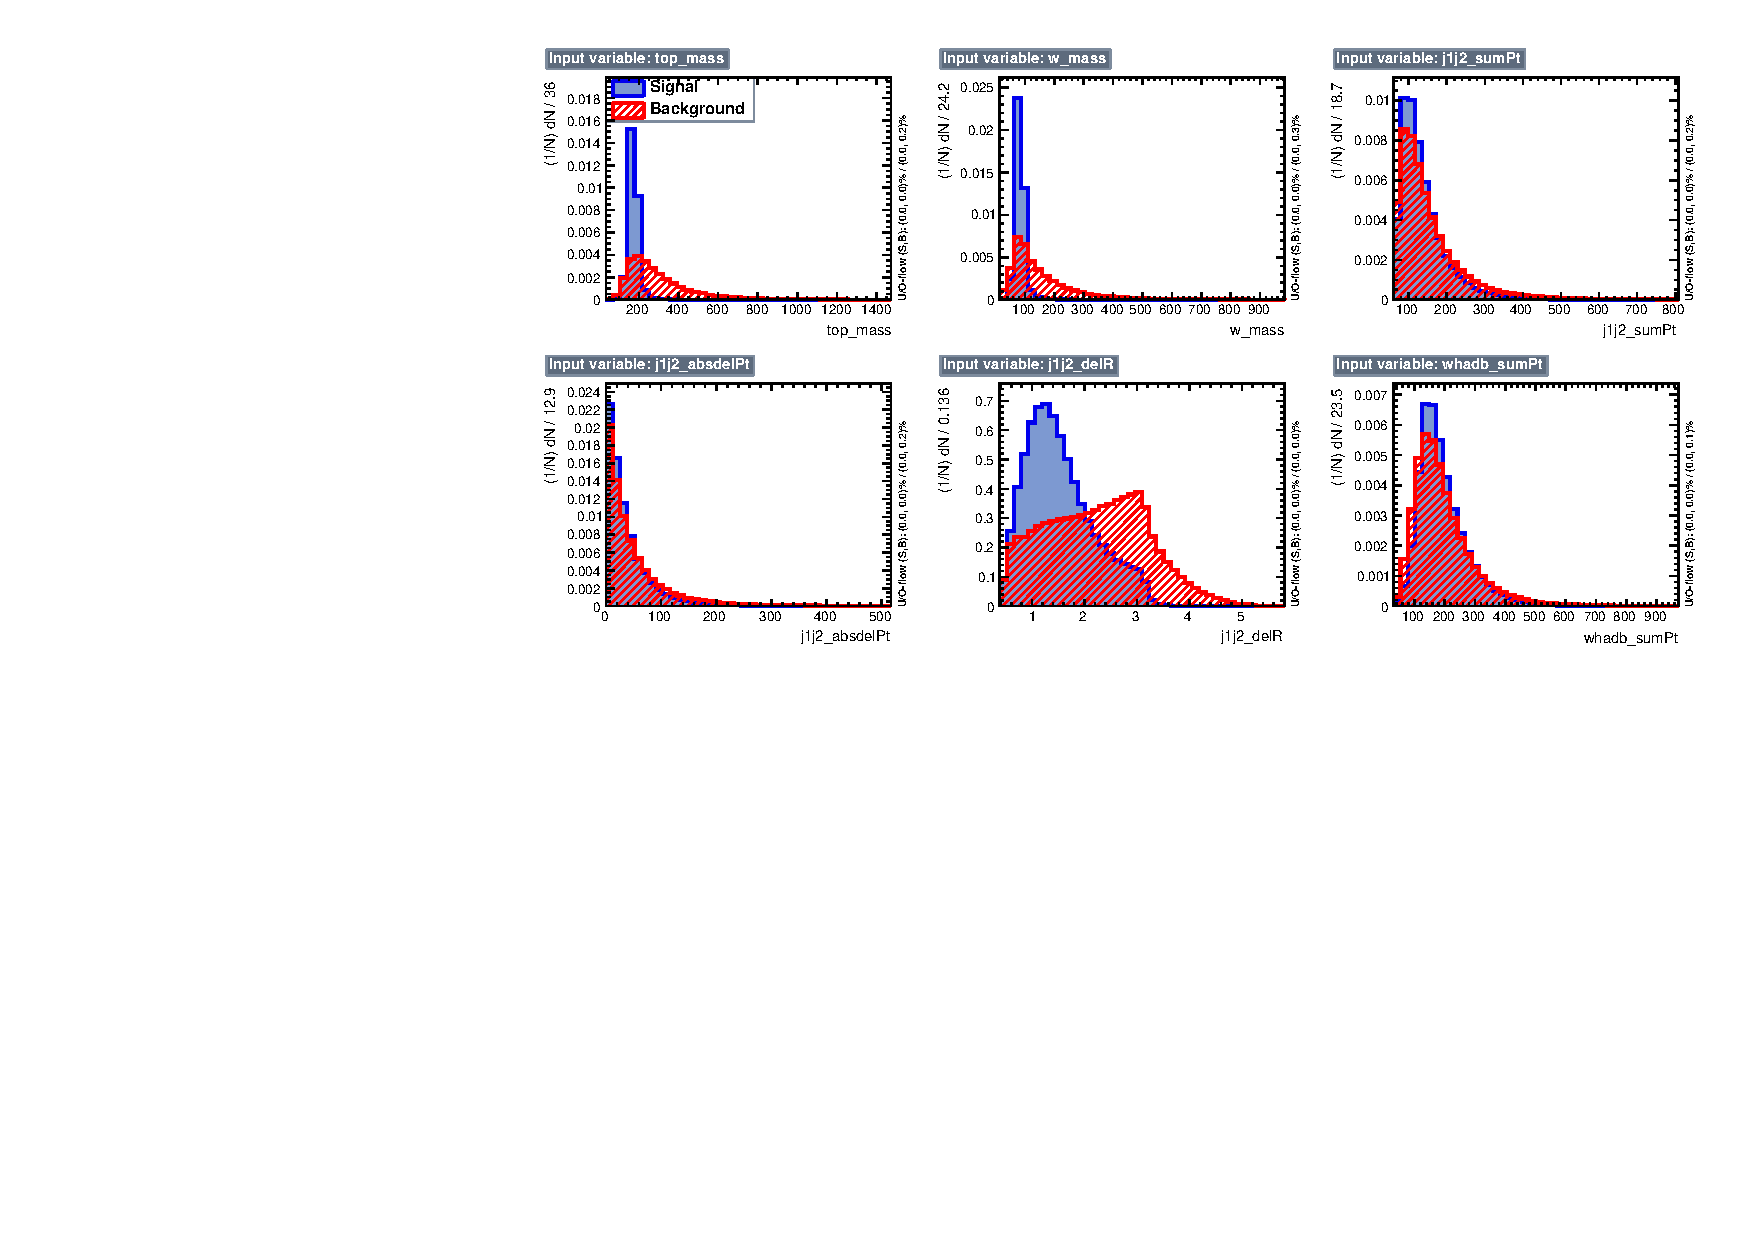
\includegraphics[width=0.8\textwidth]{Figures/EventSelReco/mva/a05_VarSep1.pdf}\\
			\end{figure}
			\FloatBarrier
			\begin{figure}[H]
			\centering{}
    			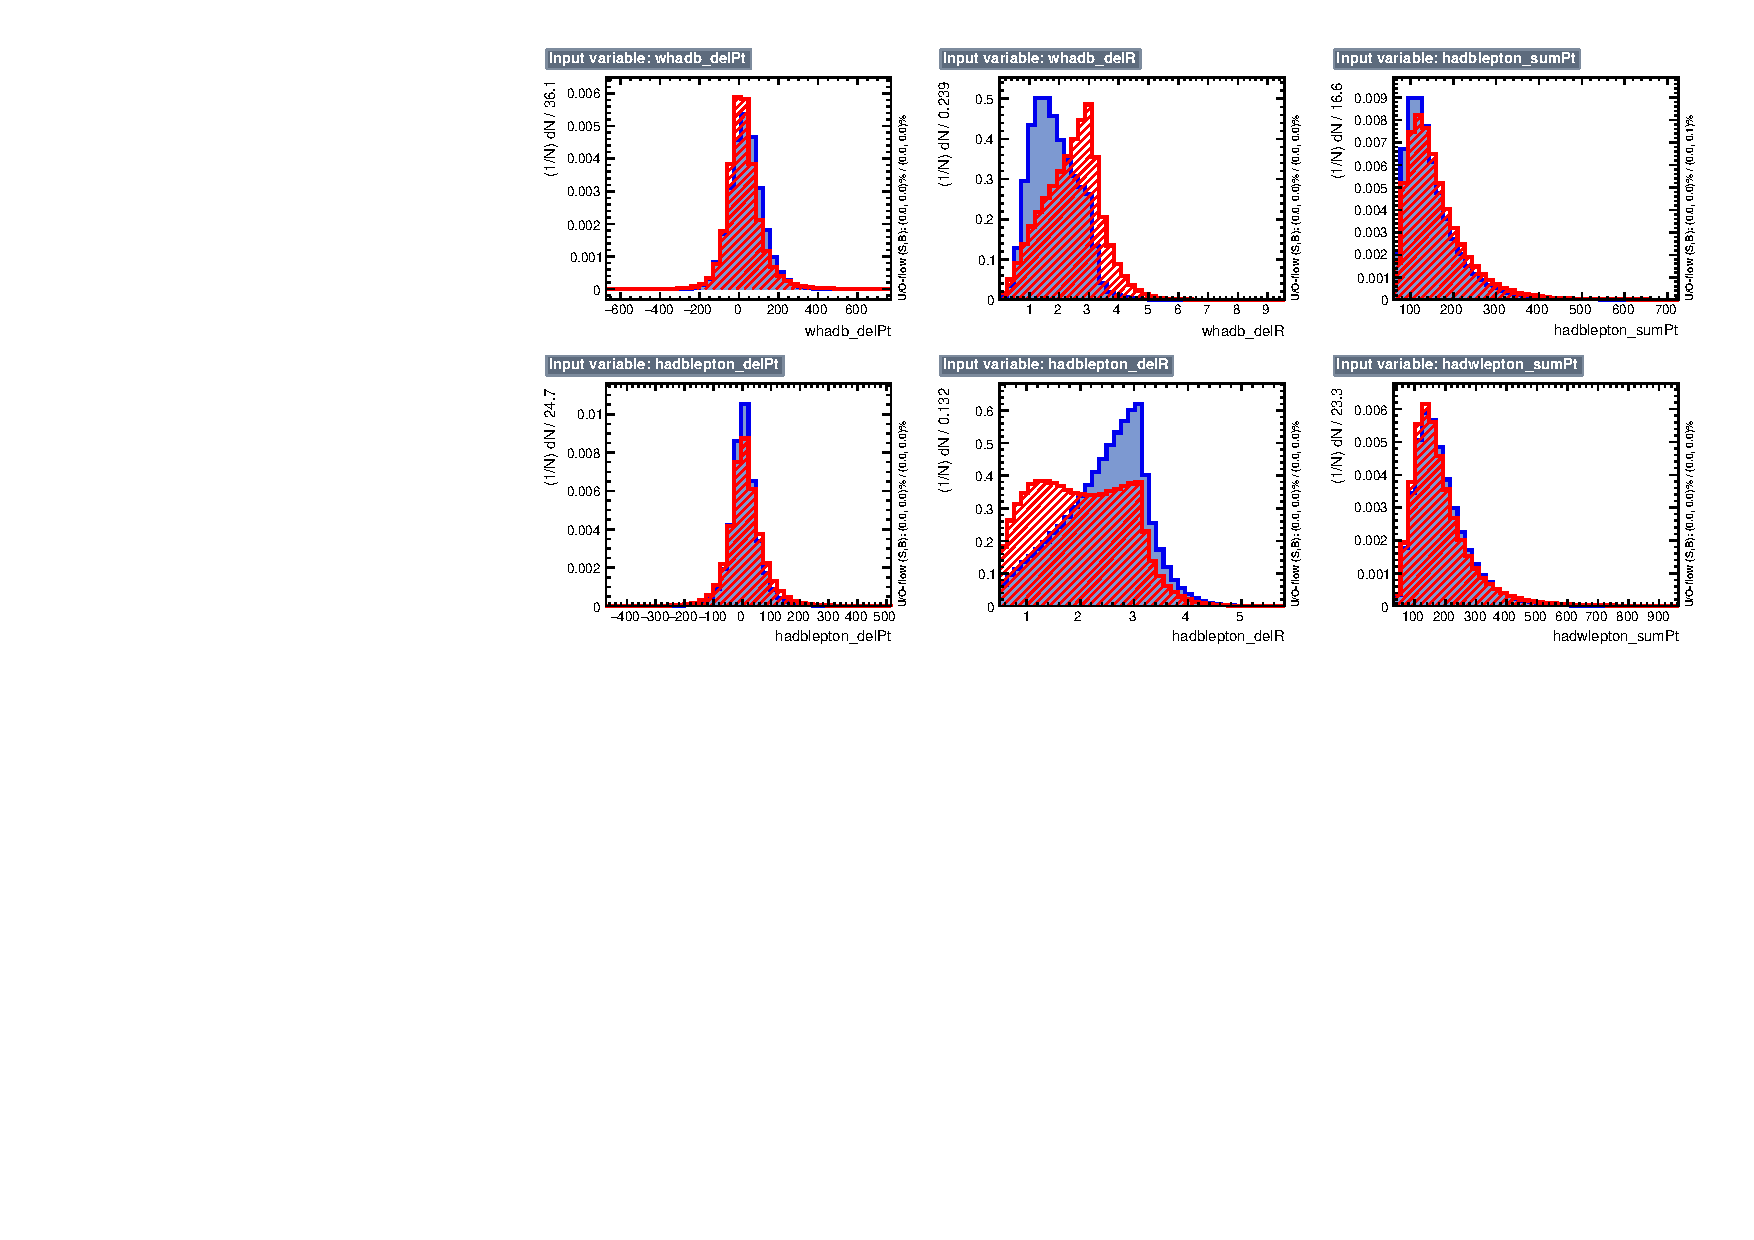
\includegraphics[width=0.8\textwidth]{Figures/EventSelReco/mva/a05_VarSep2.pdf}\\
			\end{figure}
			\FloatBarrier
			\begin{figure}[H]
			\centering{}
    			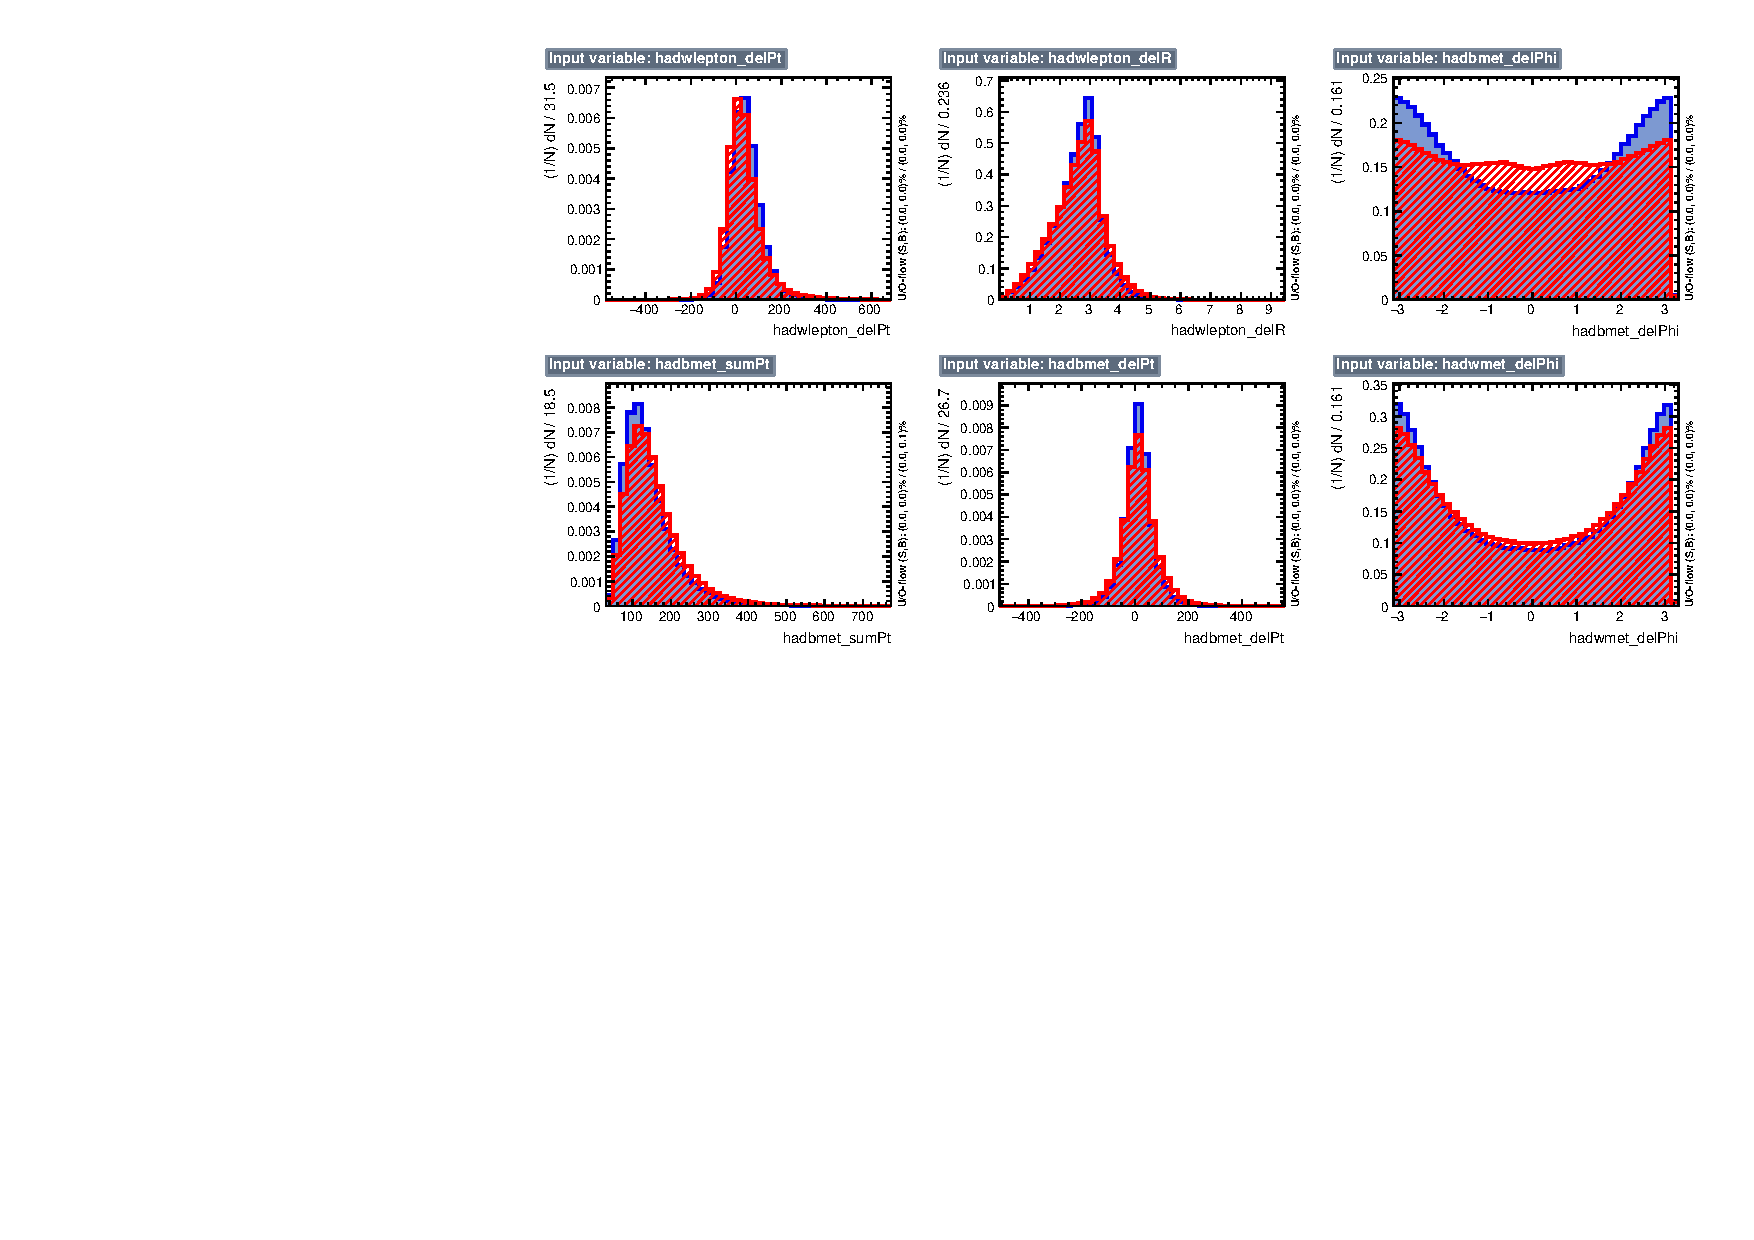
\includegraphics[width=0.8\textwidth]{Figures/EventSelReco/mva/a05_VarSep3.pdf}\\
			\end{figure}
			\FloatBarrier
			\begin{figure}[H]
			\centering{}
    			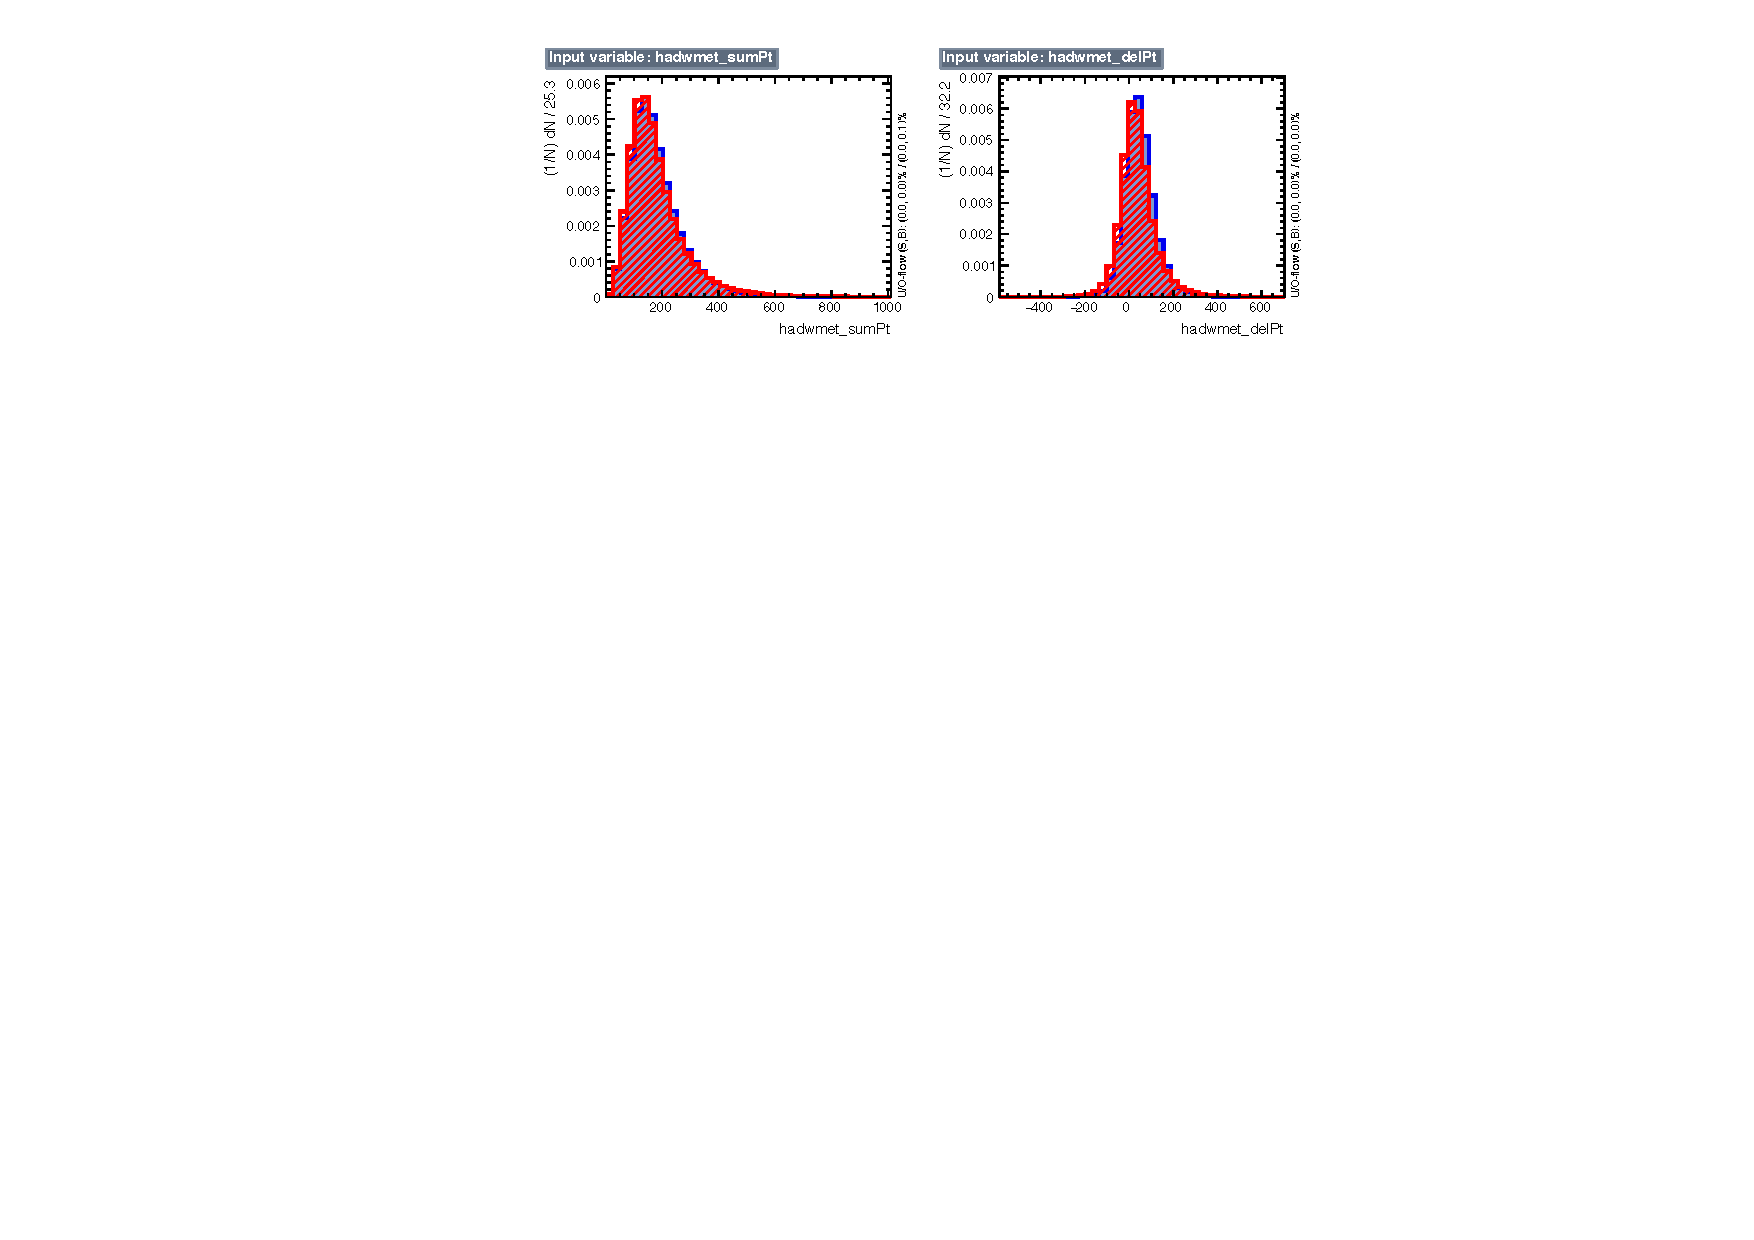
\includegraphics[width=0.528\textwidth]{Figures/EventSelReco/mva/a05_VarSep4.pdf}\\
    		\caption{Input training variables separation between $"$signal$"$ and $"$background$"$.(20 variables)}
			\label{EventSelReco:fig:a05_varsep}
			\end{figure}
			\FloatBarrier


			\begin{figure}[H]
			\centering
				\subfigure[BDT's separation result (20 vars)]{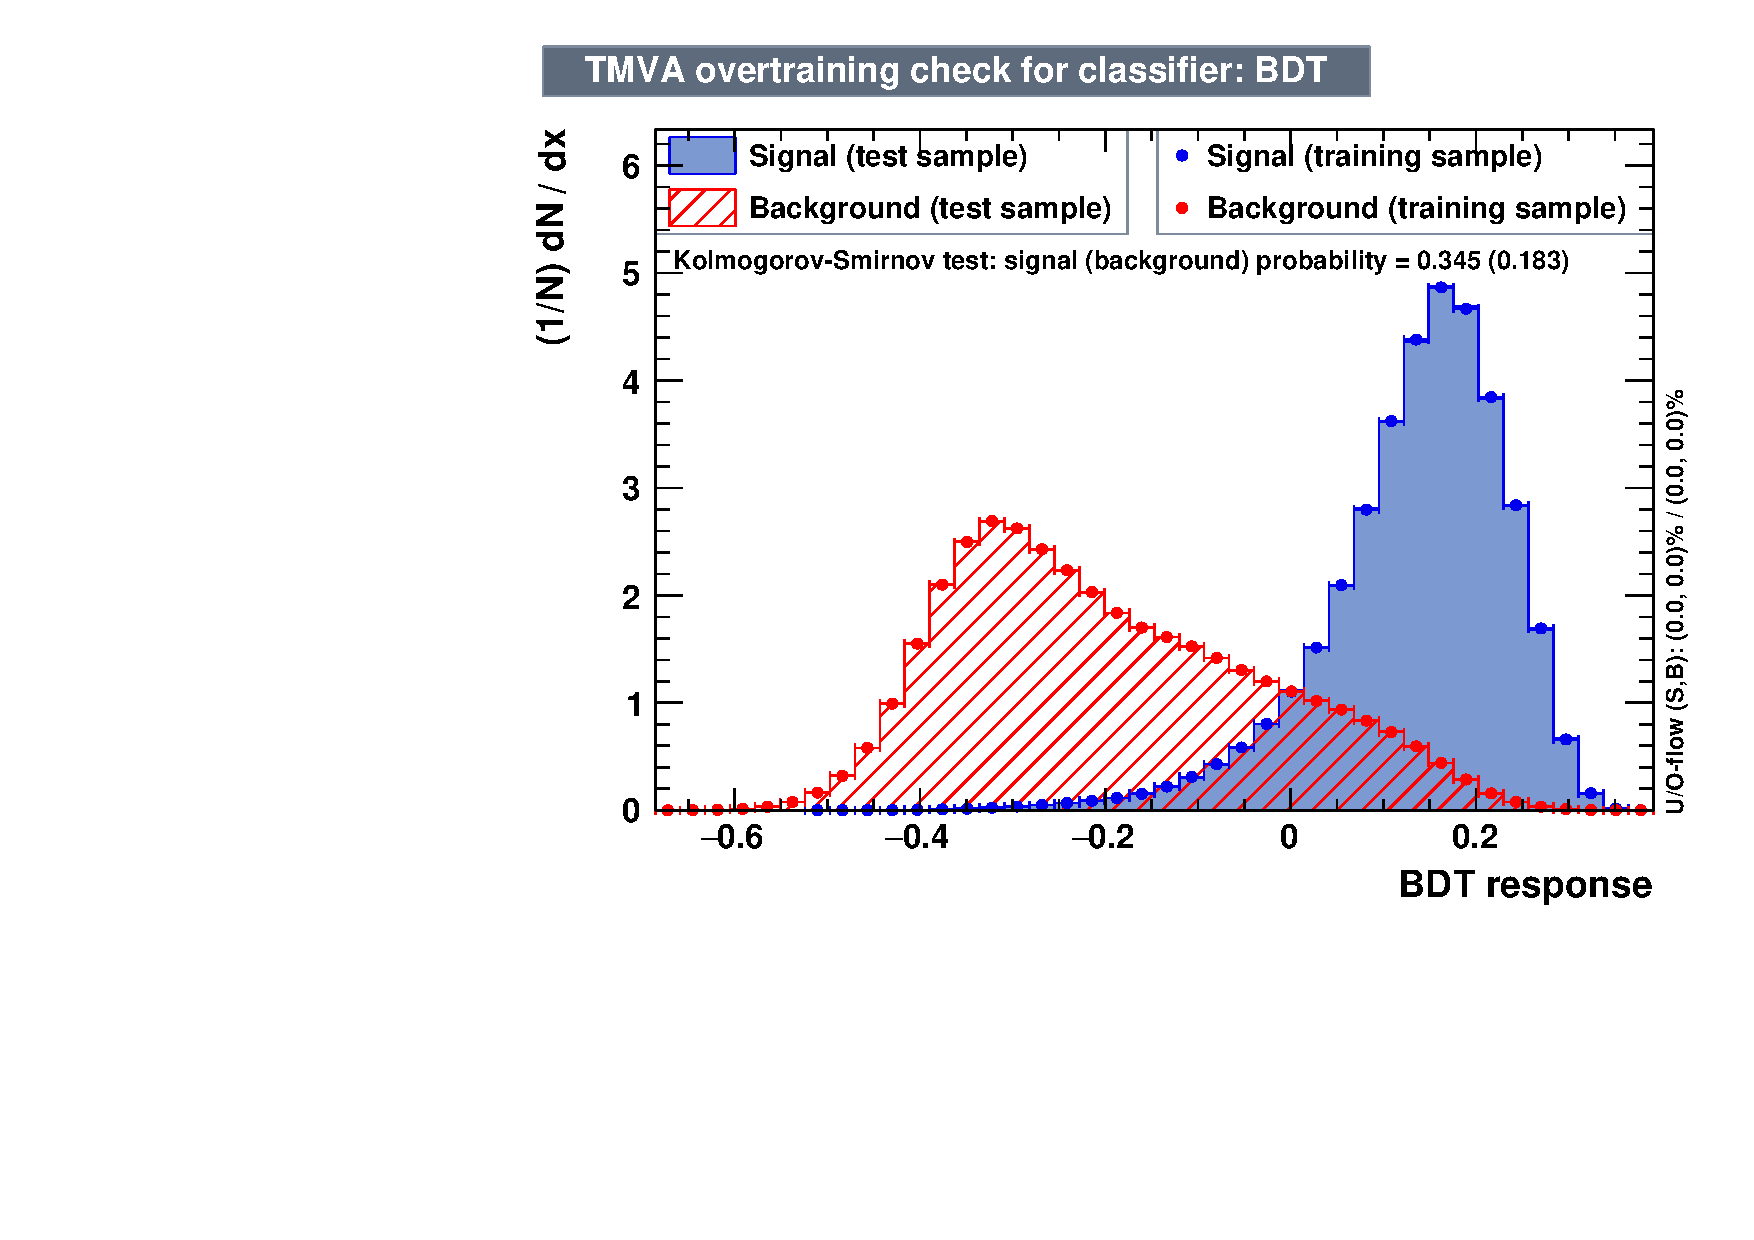
\includegraphics[width=0.4\textwidth]{Figures/EventSelReco/mva/a05_all_BDT_sep.pdf}}
			    \subfigure[BDTG's separation result (20 vars)]{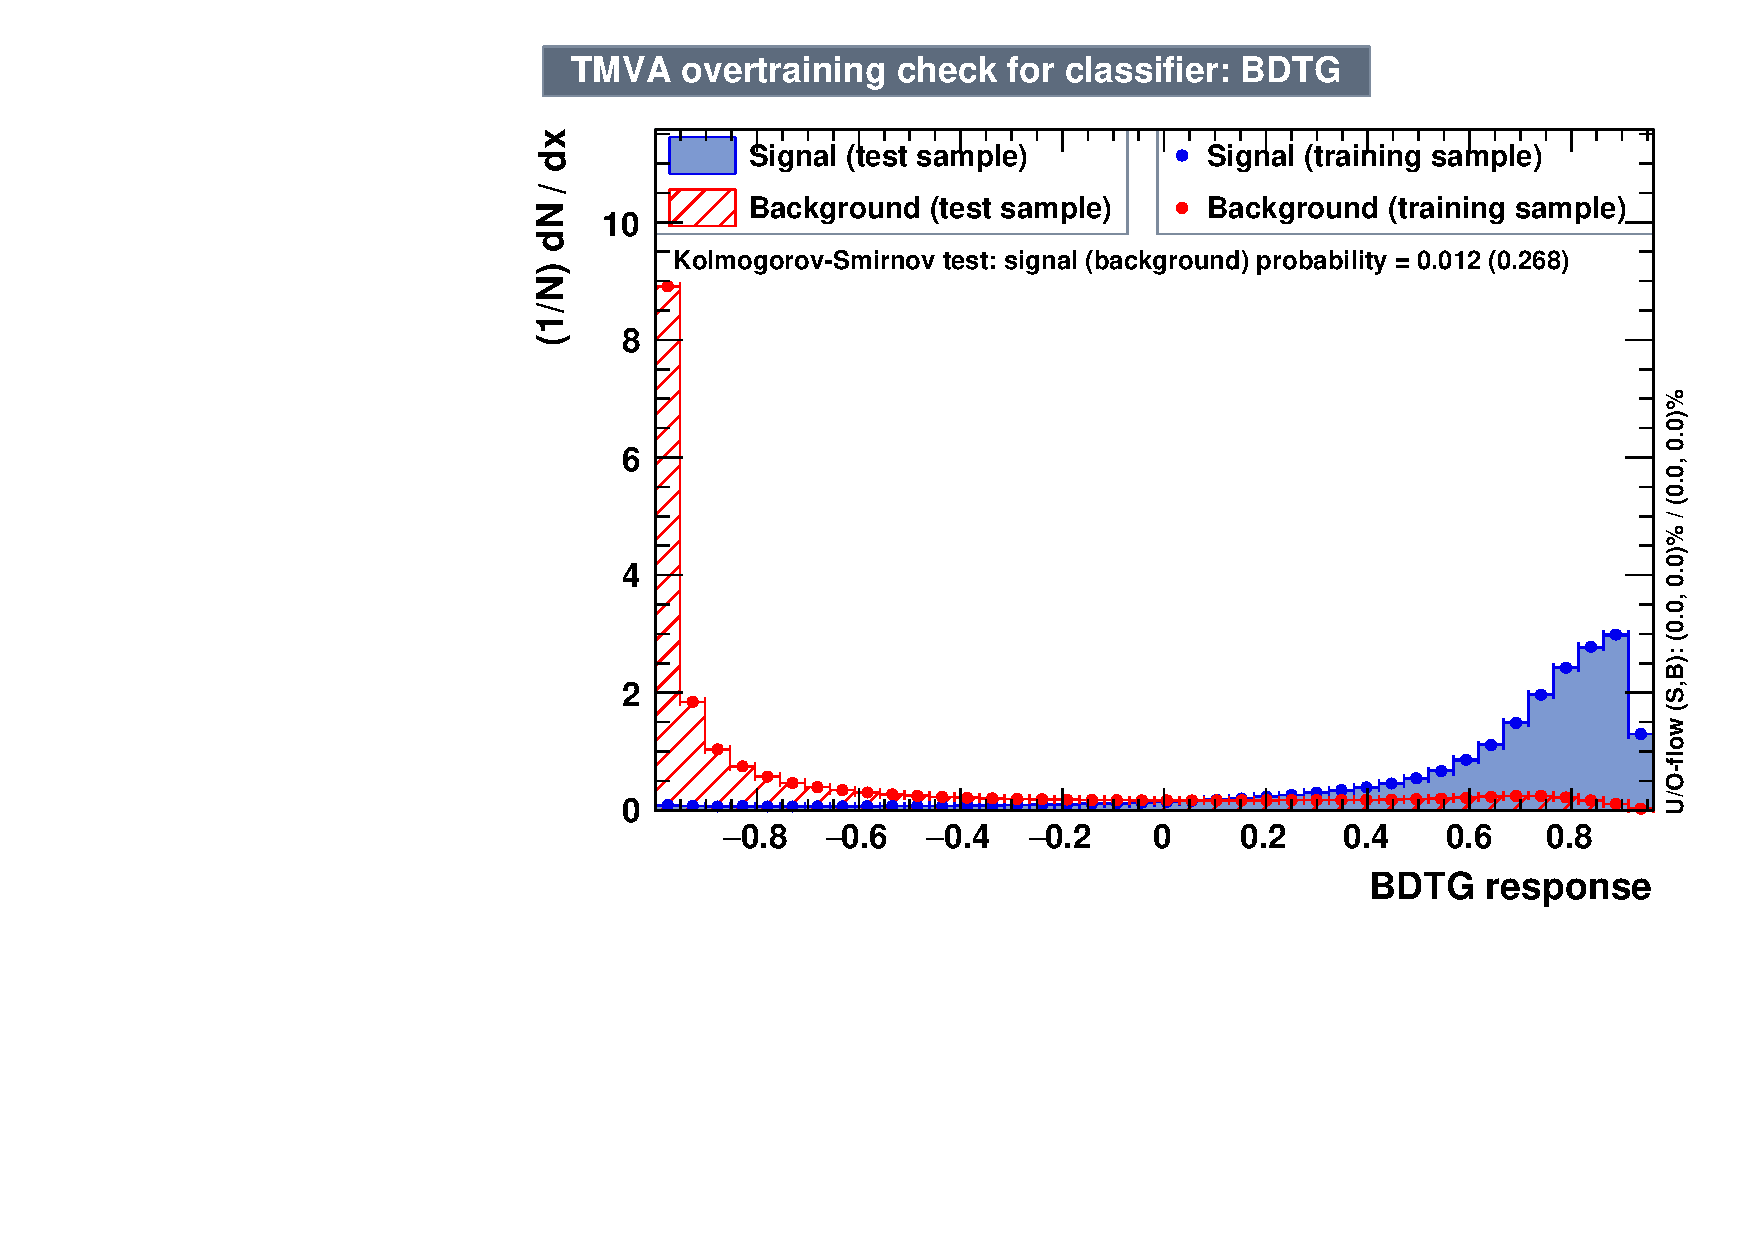
\includegraphics[width=0.4\textwidth]{Figures/EventSelReco/mva/a05_all_BDTG_sep.pdf}}\\
			\end{figure}
			\FloatBarrier
			\begin{figure}[H]
			\centering
			    \subfigure[MLP's separation result (20 vars)]{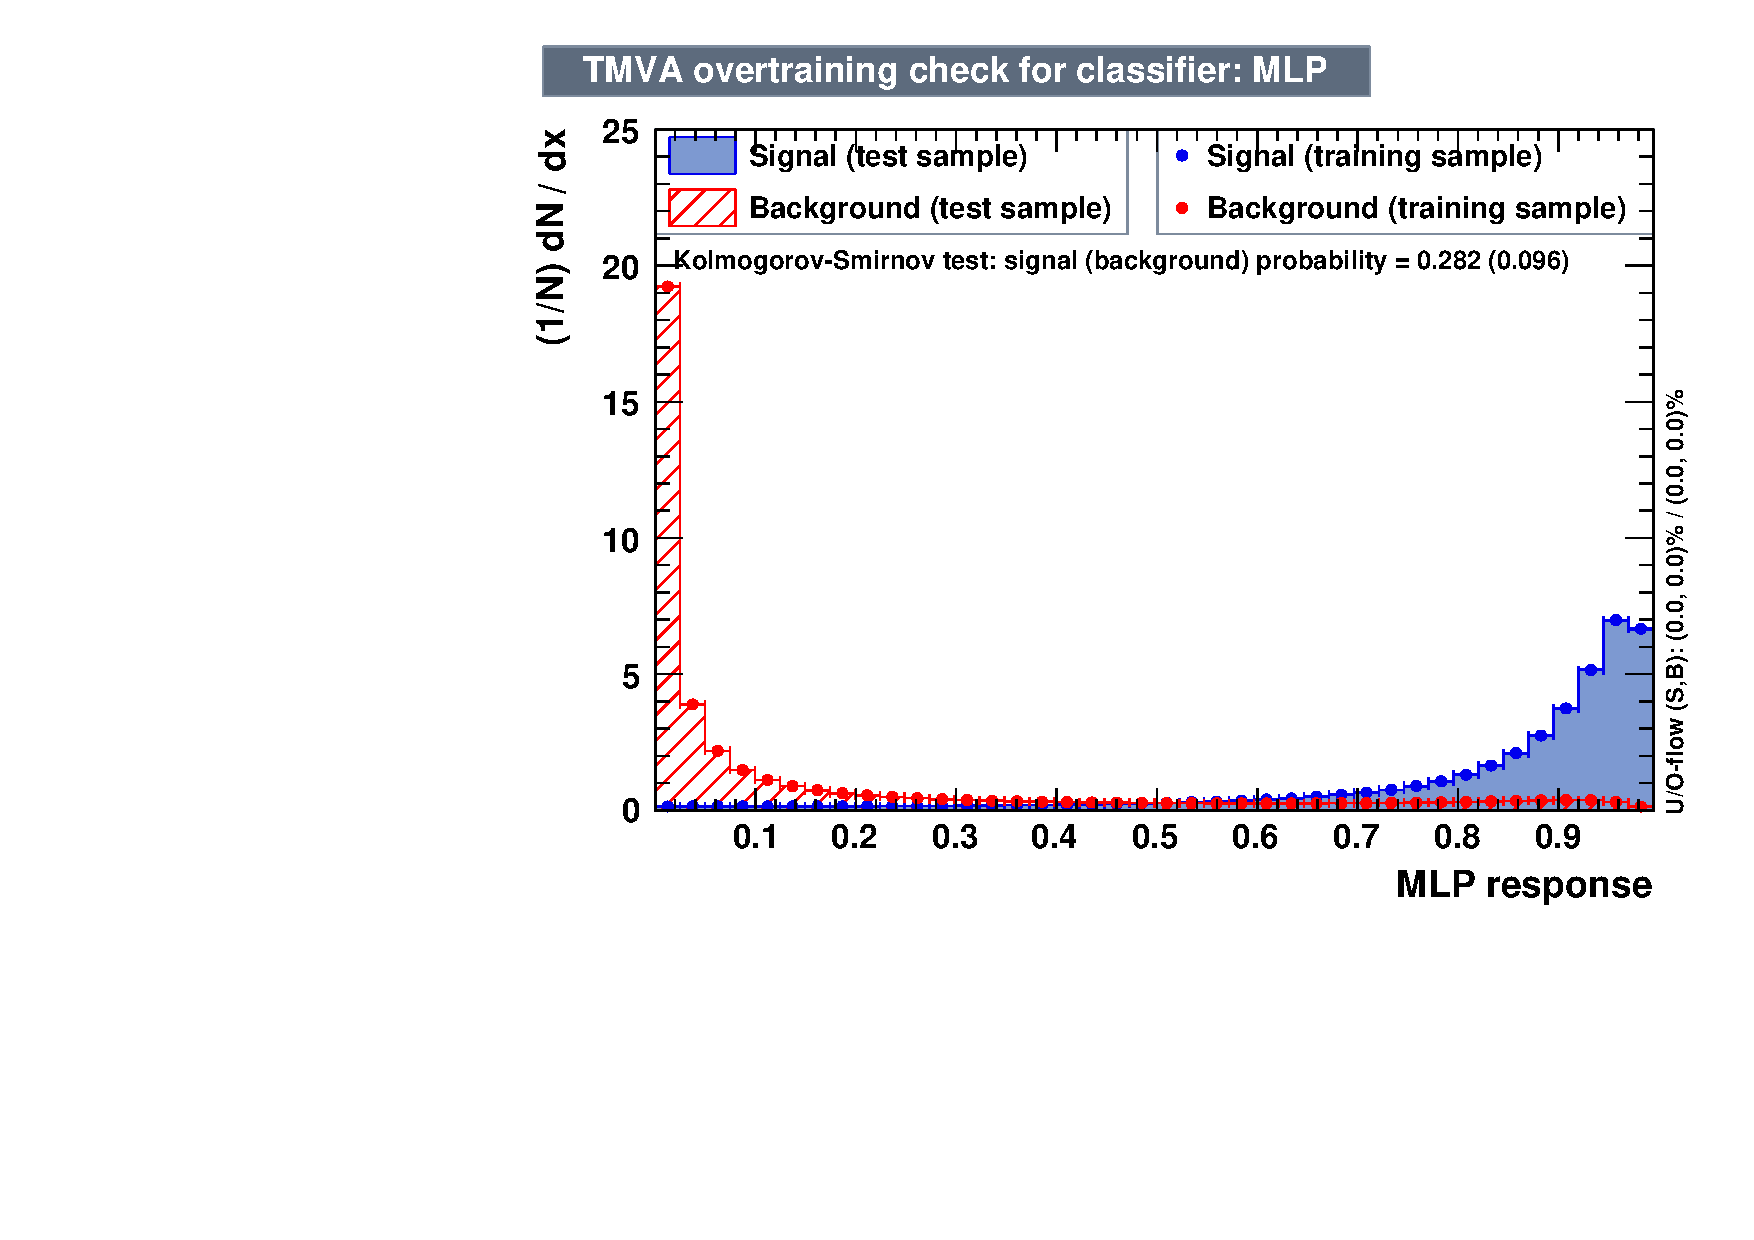
\includegraphics[width=0.4\textwidth]{Figures/EventSelReco/mva/a05_all_MLP_sep.pdf}}
			    \subfigure[ROC curve (20 vars)]{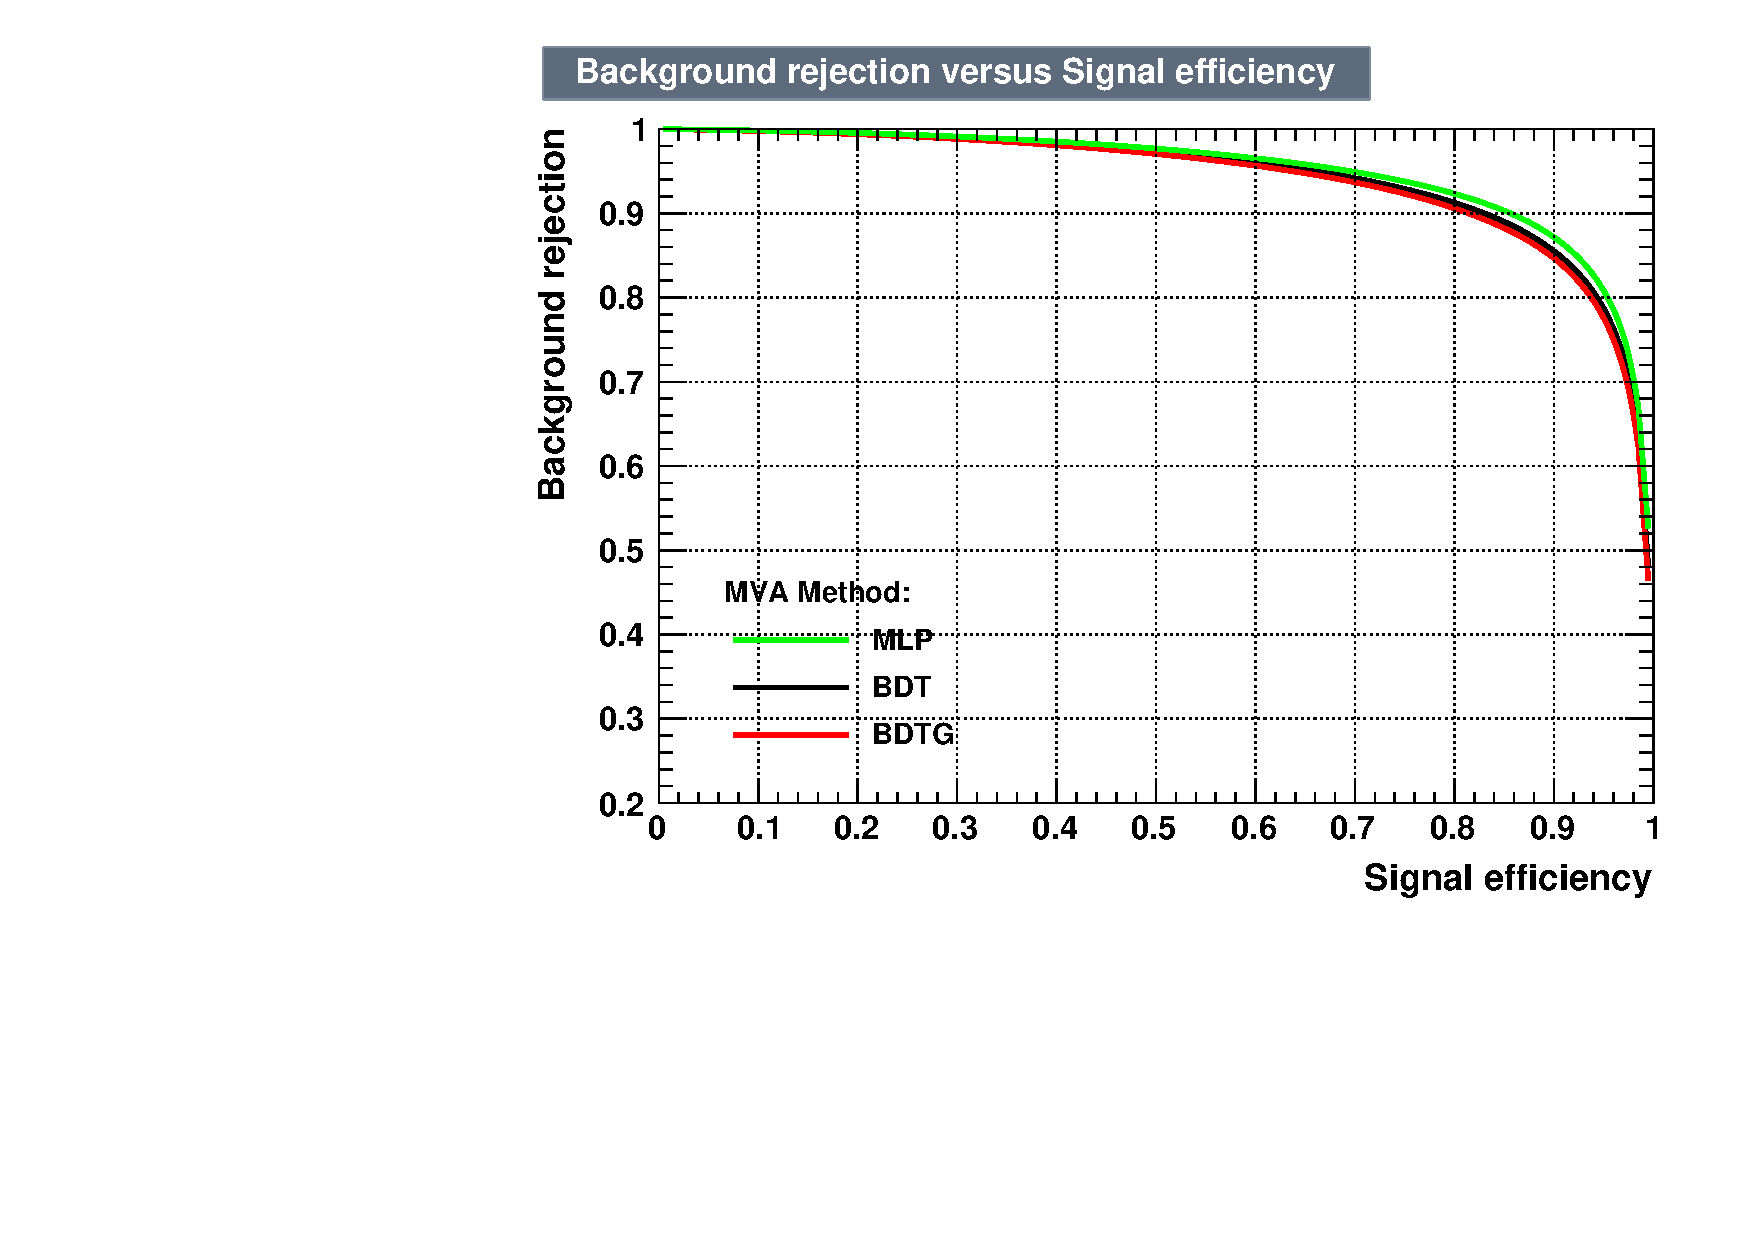
\includegraphics[width=0.4\textwidth]{Figures/EventSelReco/mva/a05_all_ROC.pdf}}\\
			\caption{The training result of 20 variables set}
			\label{EventSelReco:fig:Sep_ROC_a05}
			\end{figure}
			\FloatBarrier

			This is shown that the MLP(ANN) training algorithm has the best performance under ROC criteria from training results. But as previous mentioning, the ROC performance cannot totally represent the training performance completely in these analysis case.

			There are results of reconstructed $M_{jjb}$ by 8 variables' and 20 variables' MLP algorithm.

			\begin{figure}[H]
			\centering
				\subfigure[muon channel]{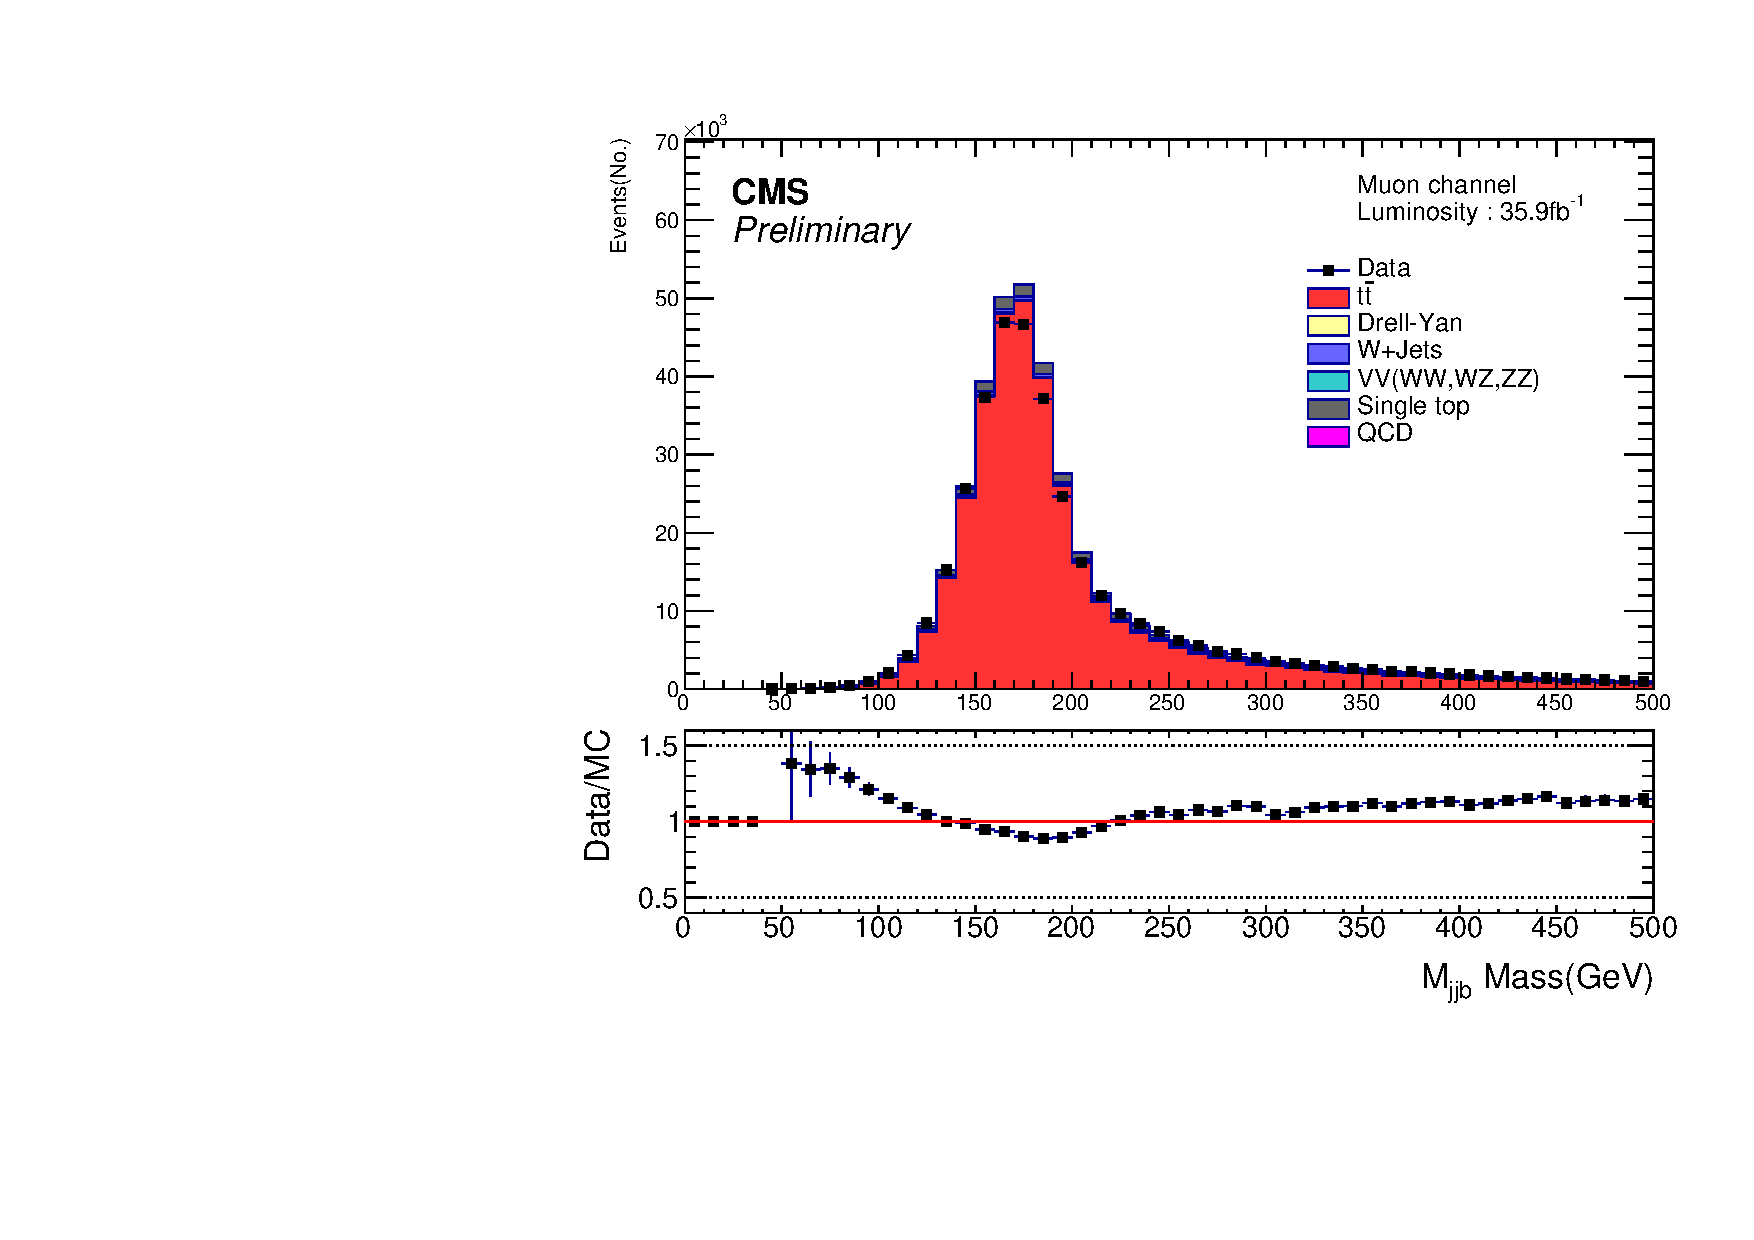
\includegraphics[width=0.45\textwidth]{Figures/EventSelReco/Mass/t13/t13_MLP_NC_long_HadTop_mu.pdf}}
			    \subfigure[electron channel]{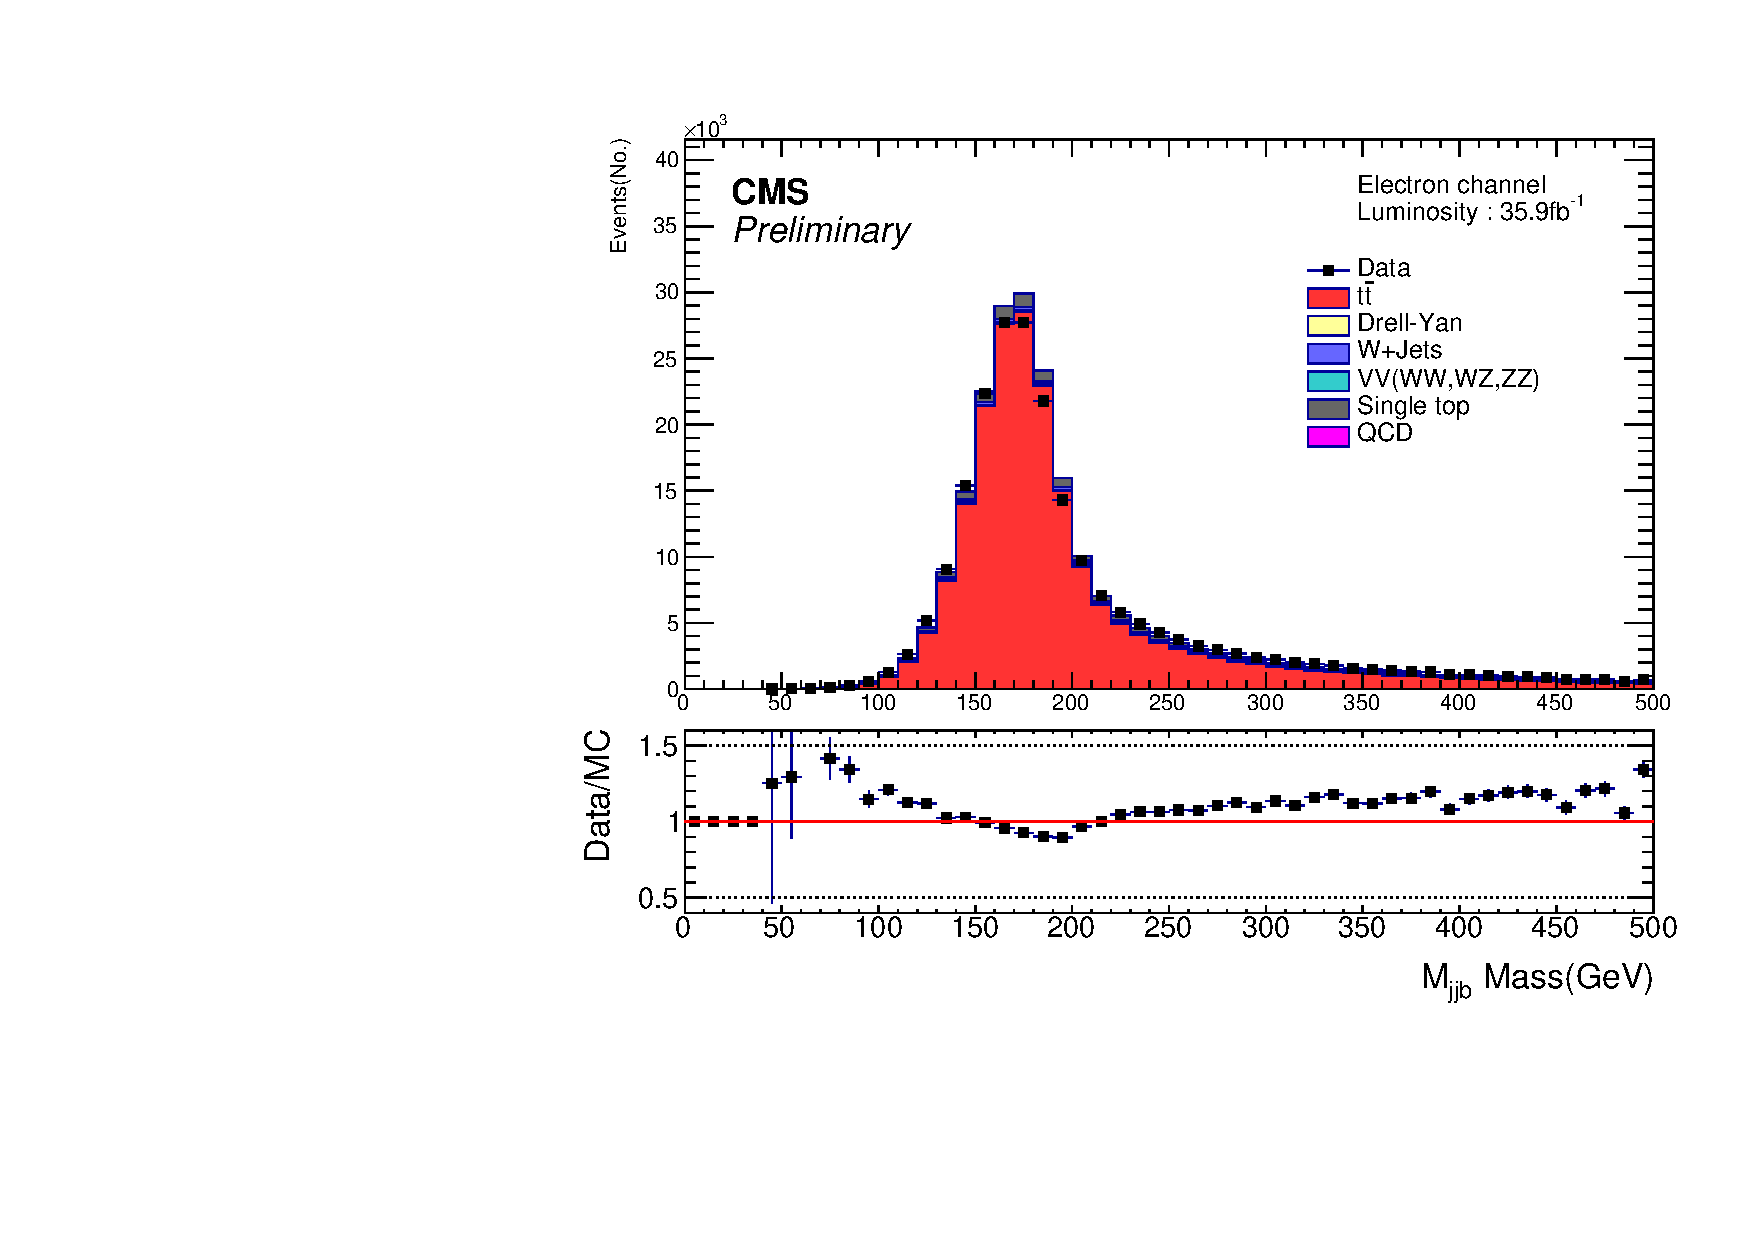
\includegraphics[width=0.45\textwidth]{Figures/EventSelReco/Mass/t13/t13_MLP_NC_long_HadTop_el.pdf}}\\
			\caption{Reconstructed $M_{jjb}$ with 8 variables MLP algorithm (w/o cut)}
			\label{EventSelReco:fig:t13_MLP_SR_NC_Mjjb}
			\end{figure}
			\FloatBarrier

			\begin{figure}[H]
			\centering
				\subfigure[muon channel]{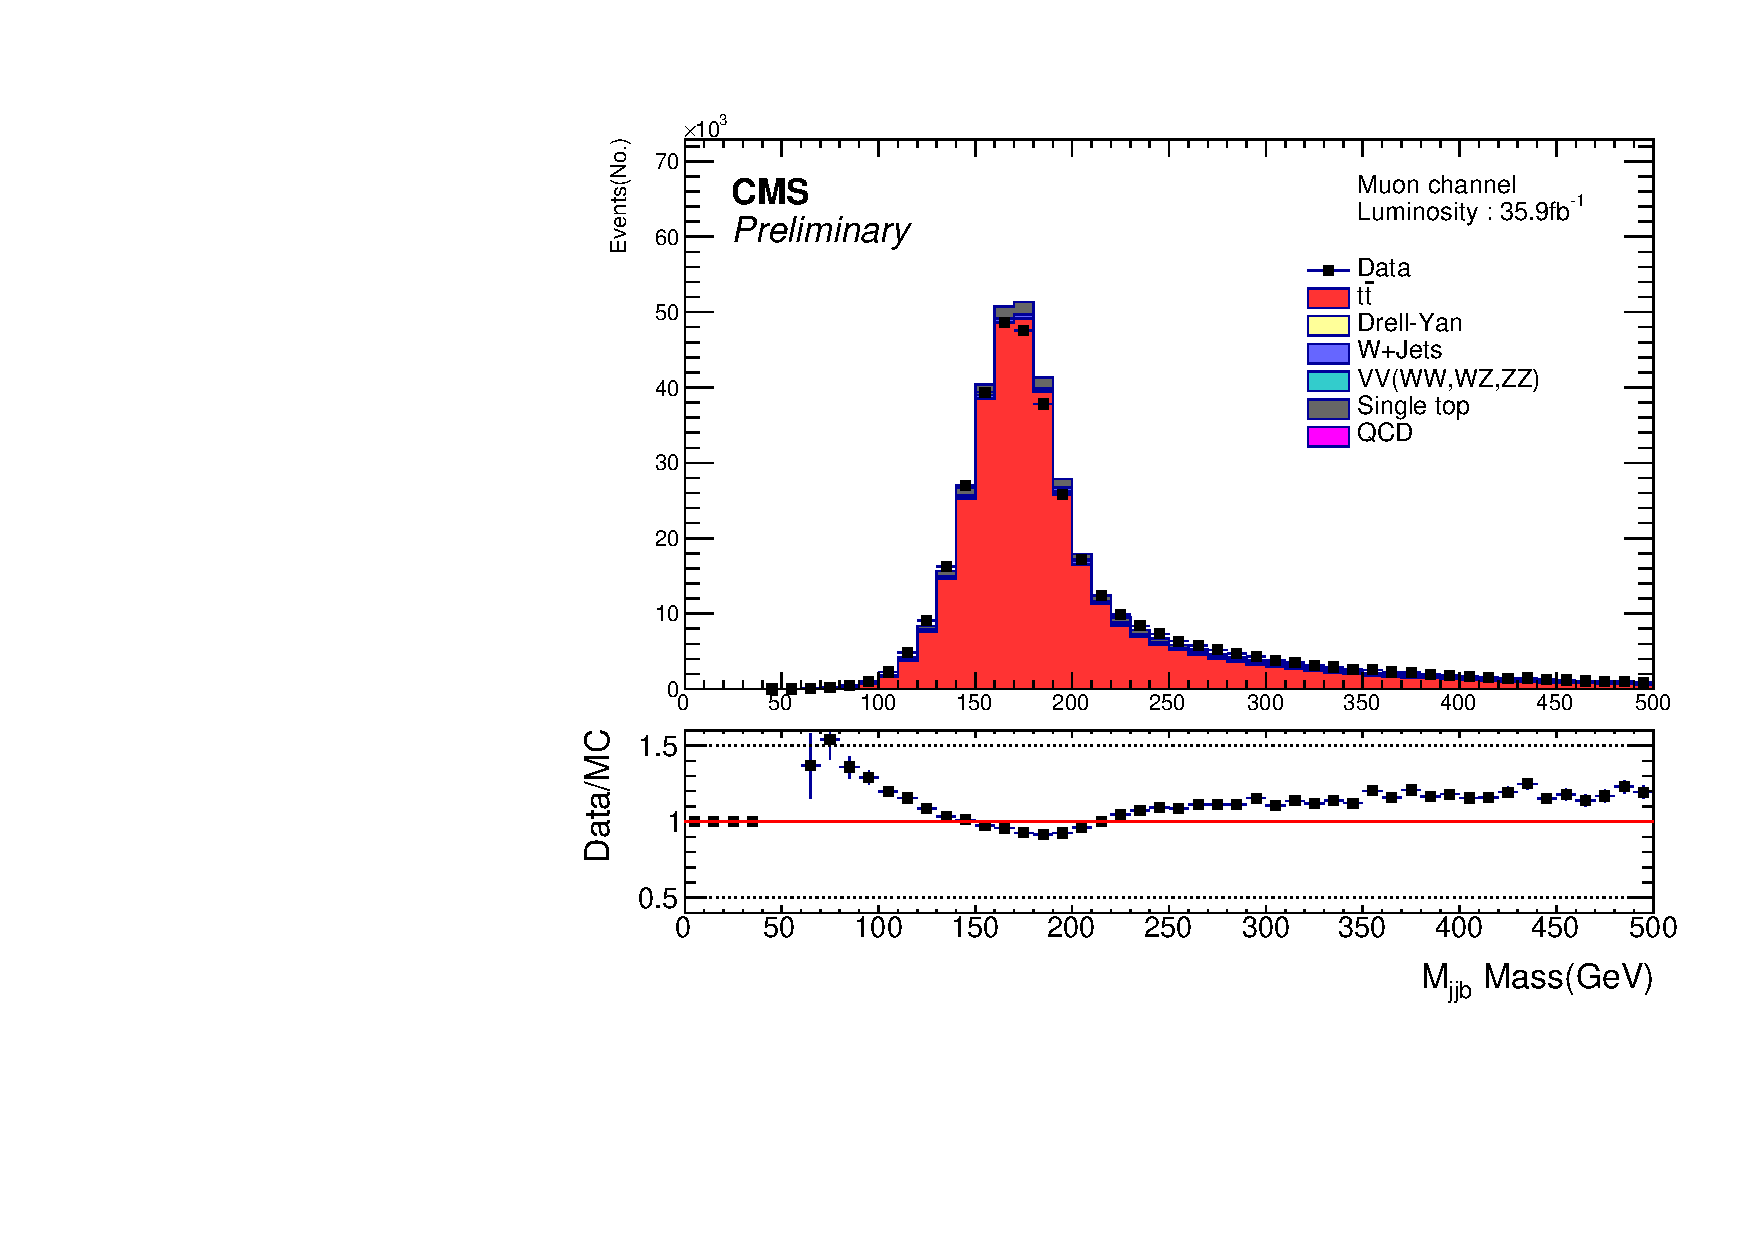
\includegraphics[width=0.45\textwidth]{Figures/EventSelReco/Mass/a05/a05_MLP_NC_long_HadTop_mu.pdf}}
			    \subfigure[electron channel]{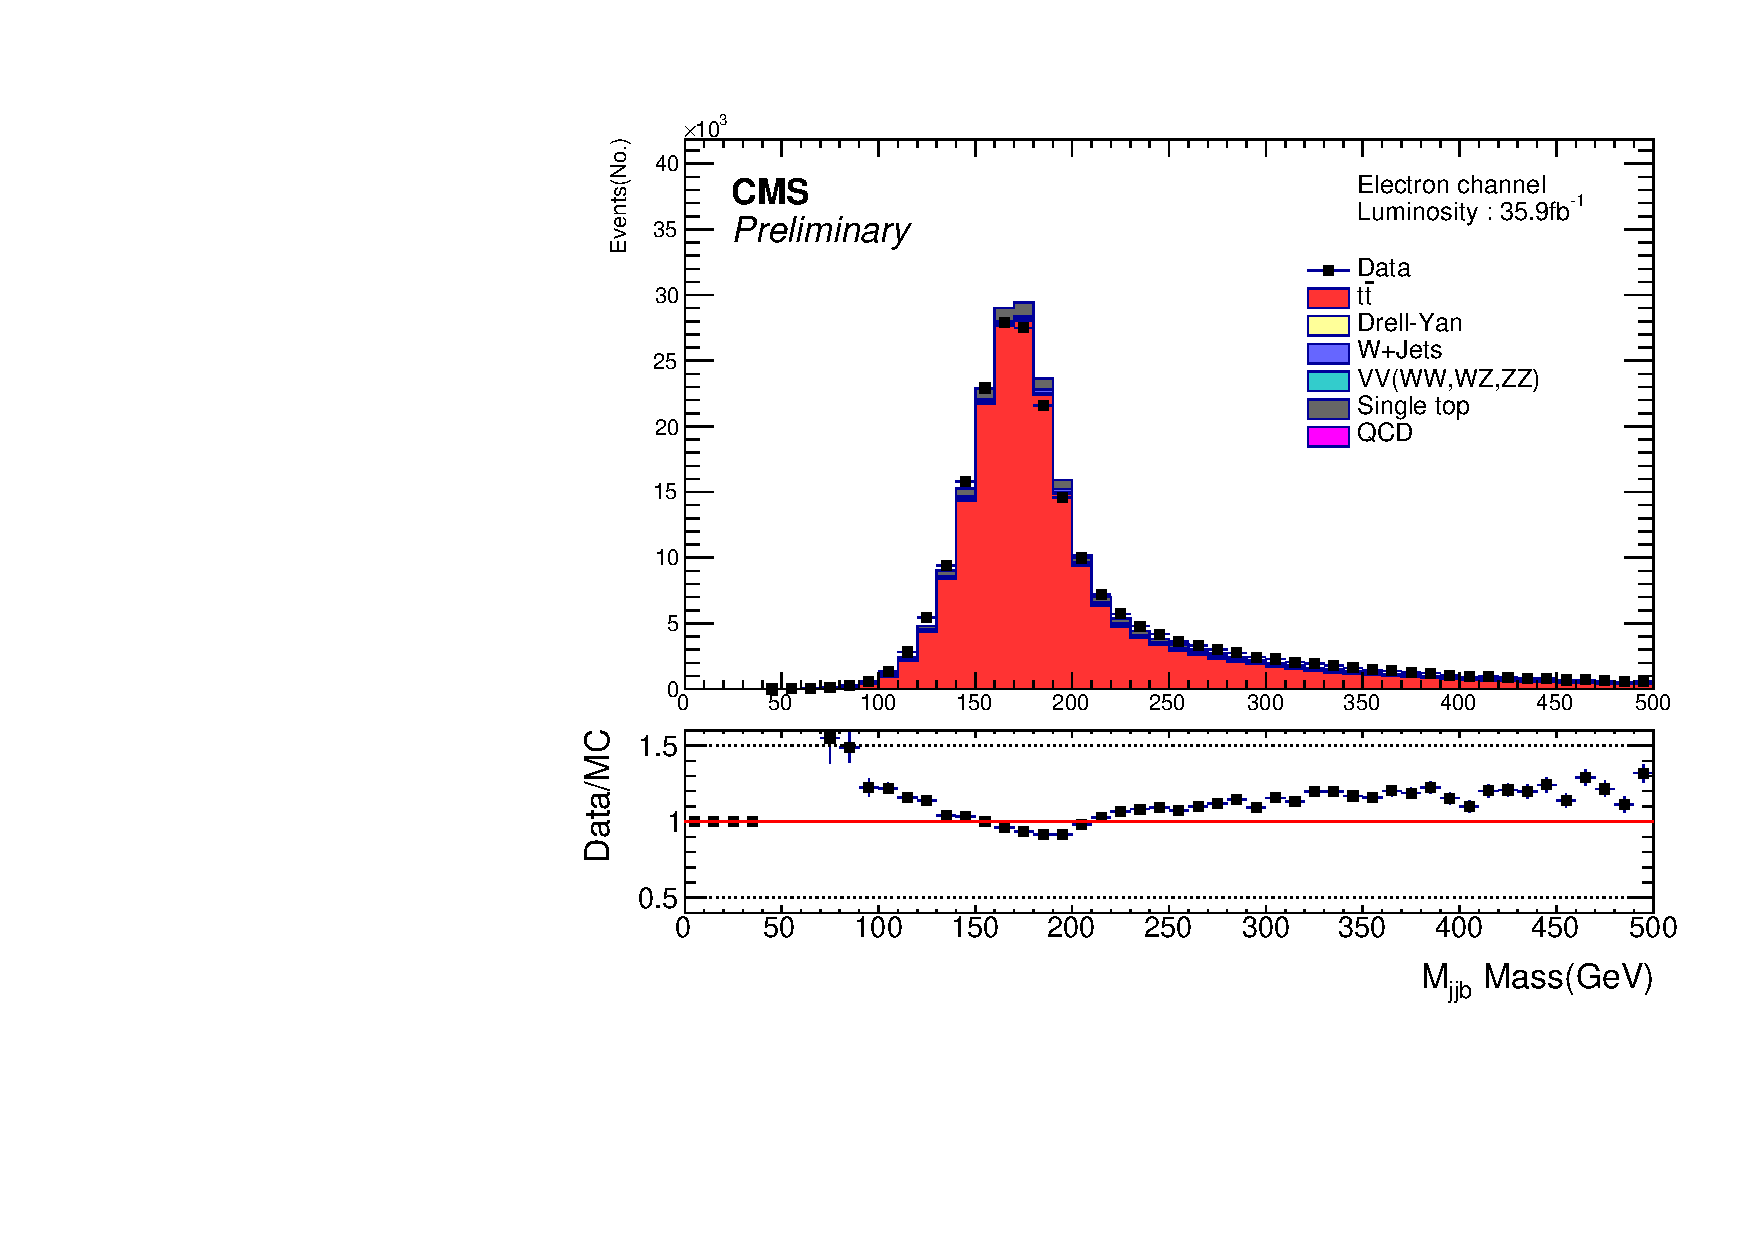
\includegraphics[width=0.45\textwidth]{Figures/EventSelReco/Mass/a05/a05_MLP_NC_long_HadTop_el.pdf}}\\
			\caption{Reconstructed $M_{jjb}$ with 20 variables MLP algorithm (w/o cut)}
			\label{EventSelReco:fig:a05_MLP_SR_NC_Mjjb}
			\end{figure}
			\FloatBarrier

			There are the max MVA score's distribution with 2/8/20 variables and BDT/BDTG/MLP results.

			\begin{figure}[H]
			\centering
				\subfigure[BDT (2 vars, mu-ch)]{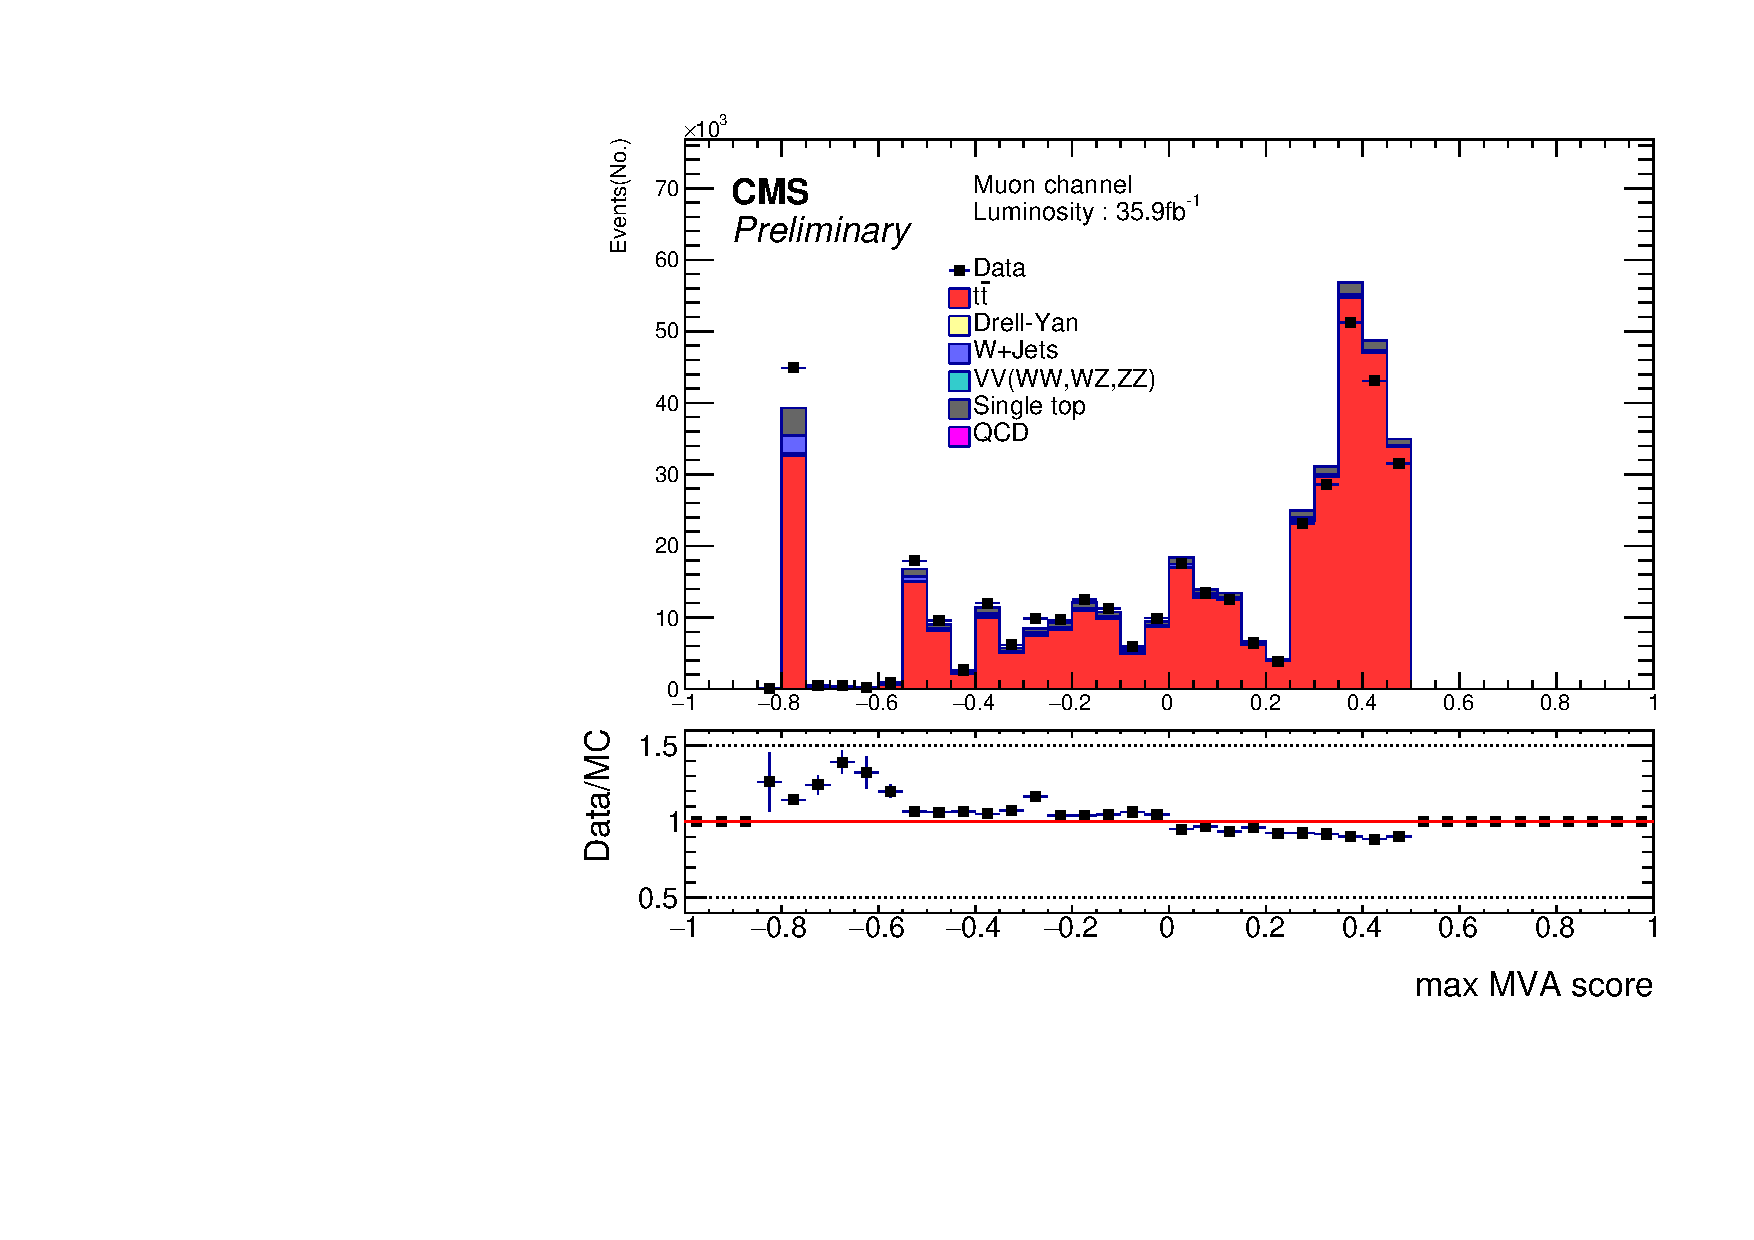
\includegraphics[width=0.32\textwidth]{Figures/EventSelReco/mva_algo/a04_BDT_SR_algo_mu.pdf}}
			    \subfigure[BDTG (2 vars, mu-ch)]{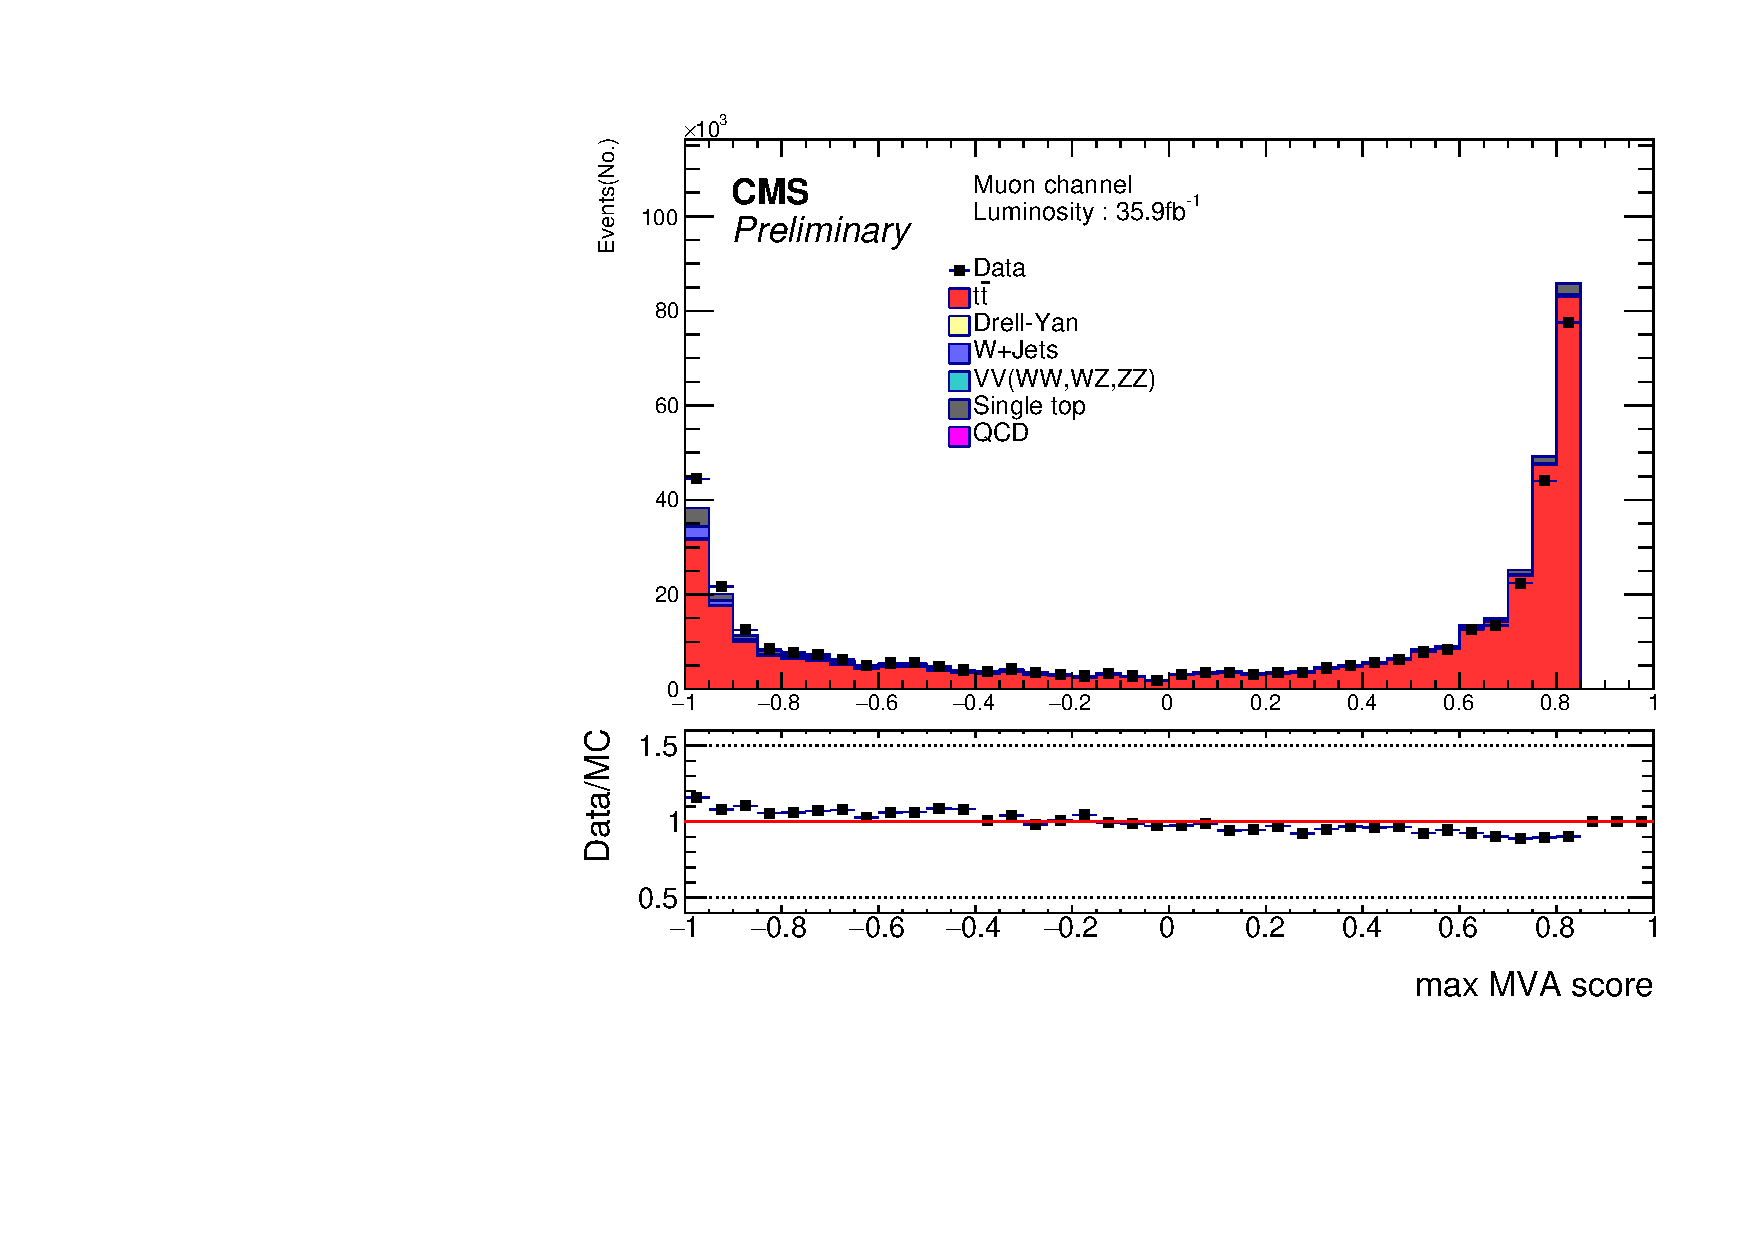
\includegraphics[width=0.32\textwidth]{Figures/EventSelReco/mva_algo/a04_BDTG_SR_algo_mu.pdf}}
			    \subfigure[MLP (2 vars, mu-ch)]{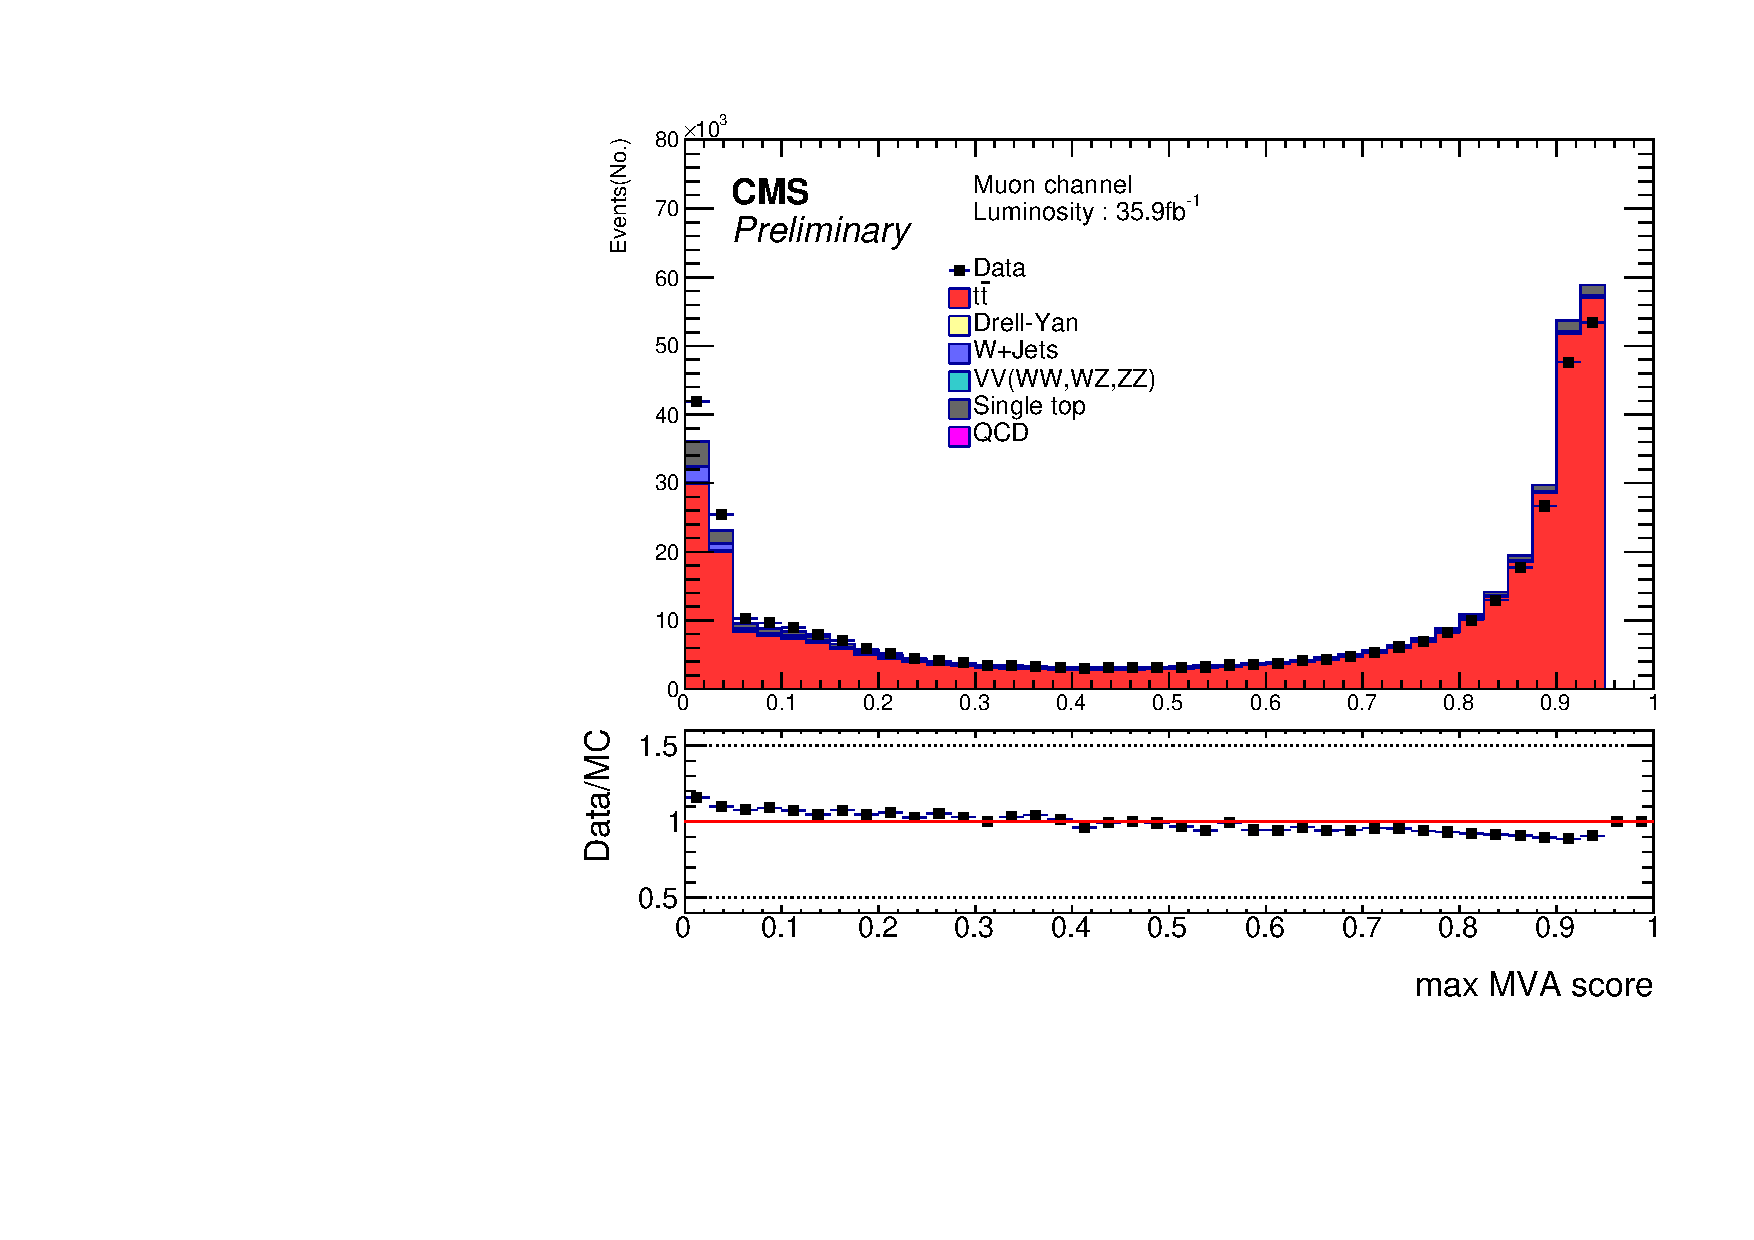
\includegraphics[width=0.32\textwidth]{Figures/EventSelReco/mva_algo/a04_MLP_SR_algo_mu.pdf}}\\
			\end{figure}
			\FloatBarrier
			\begin{figure}[H]
			\centering
			    \subfigure[BDT (2 vars, el-ch)]{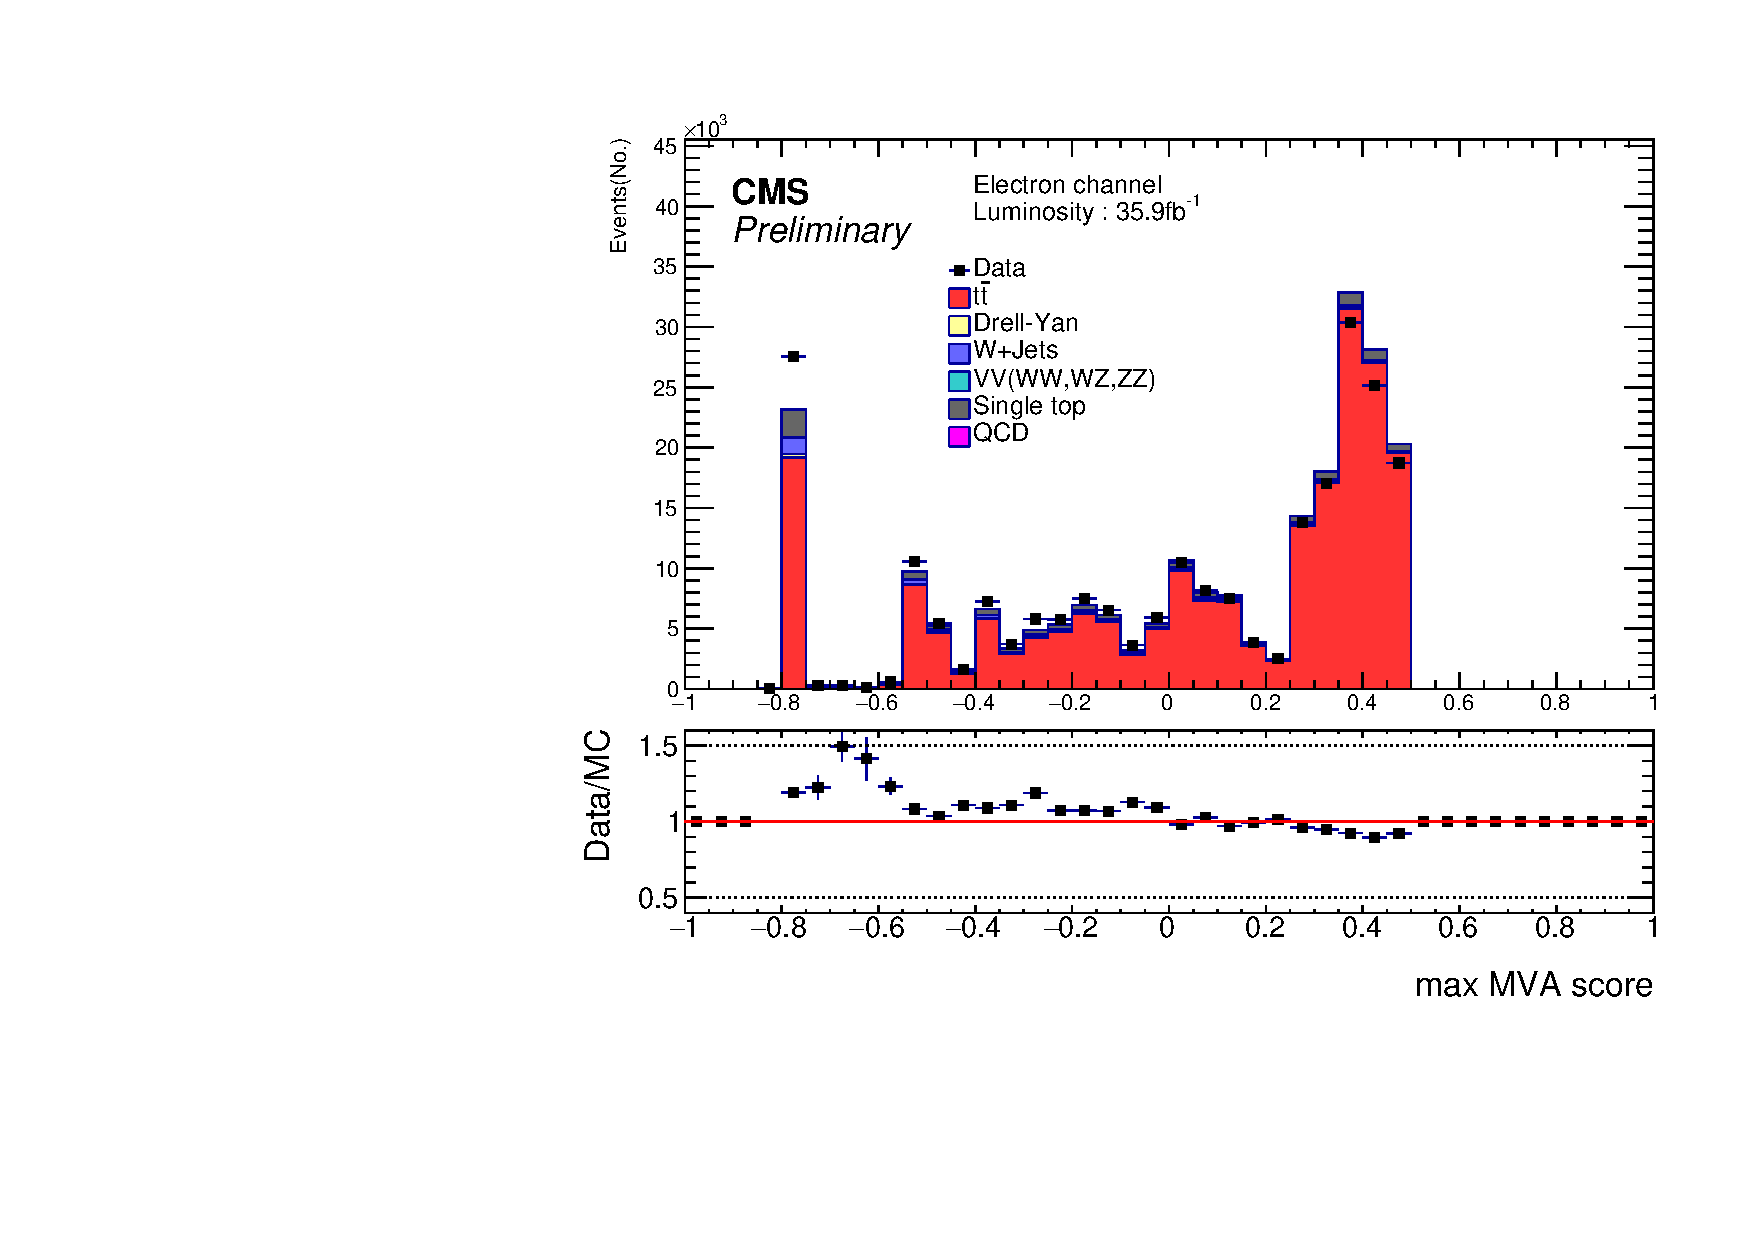
\includegraphics[width=0.32\textwidth]{Figures/EventSelReco/mva_algo/a04_BDT_SR_algo_el.pdf}}
			    \subfigure[BDTG (2 vars, el-ch)]{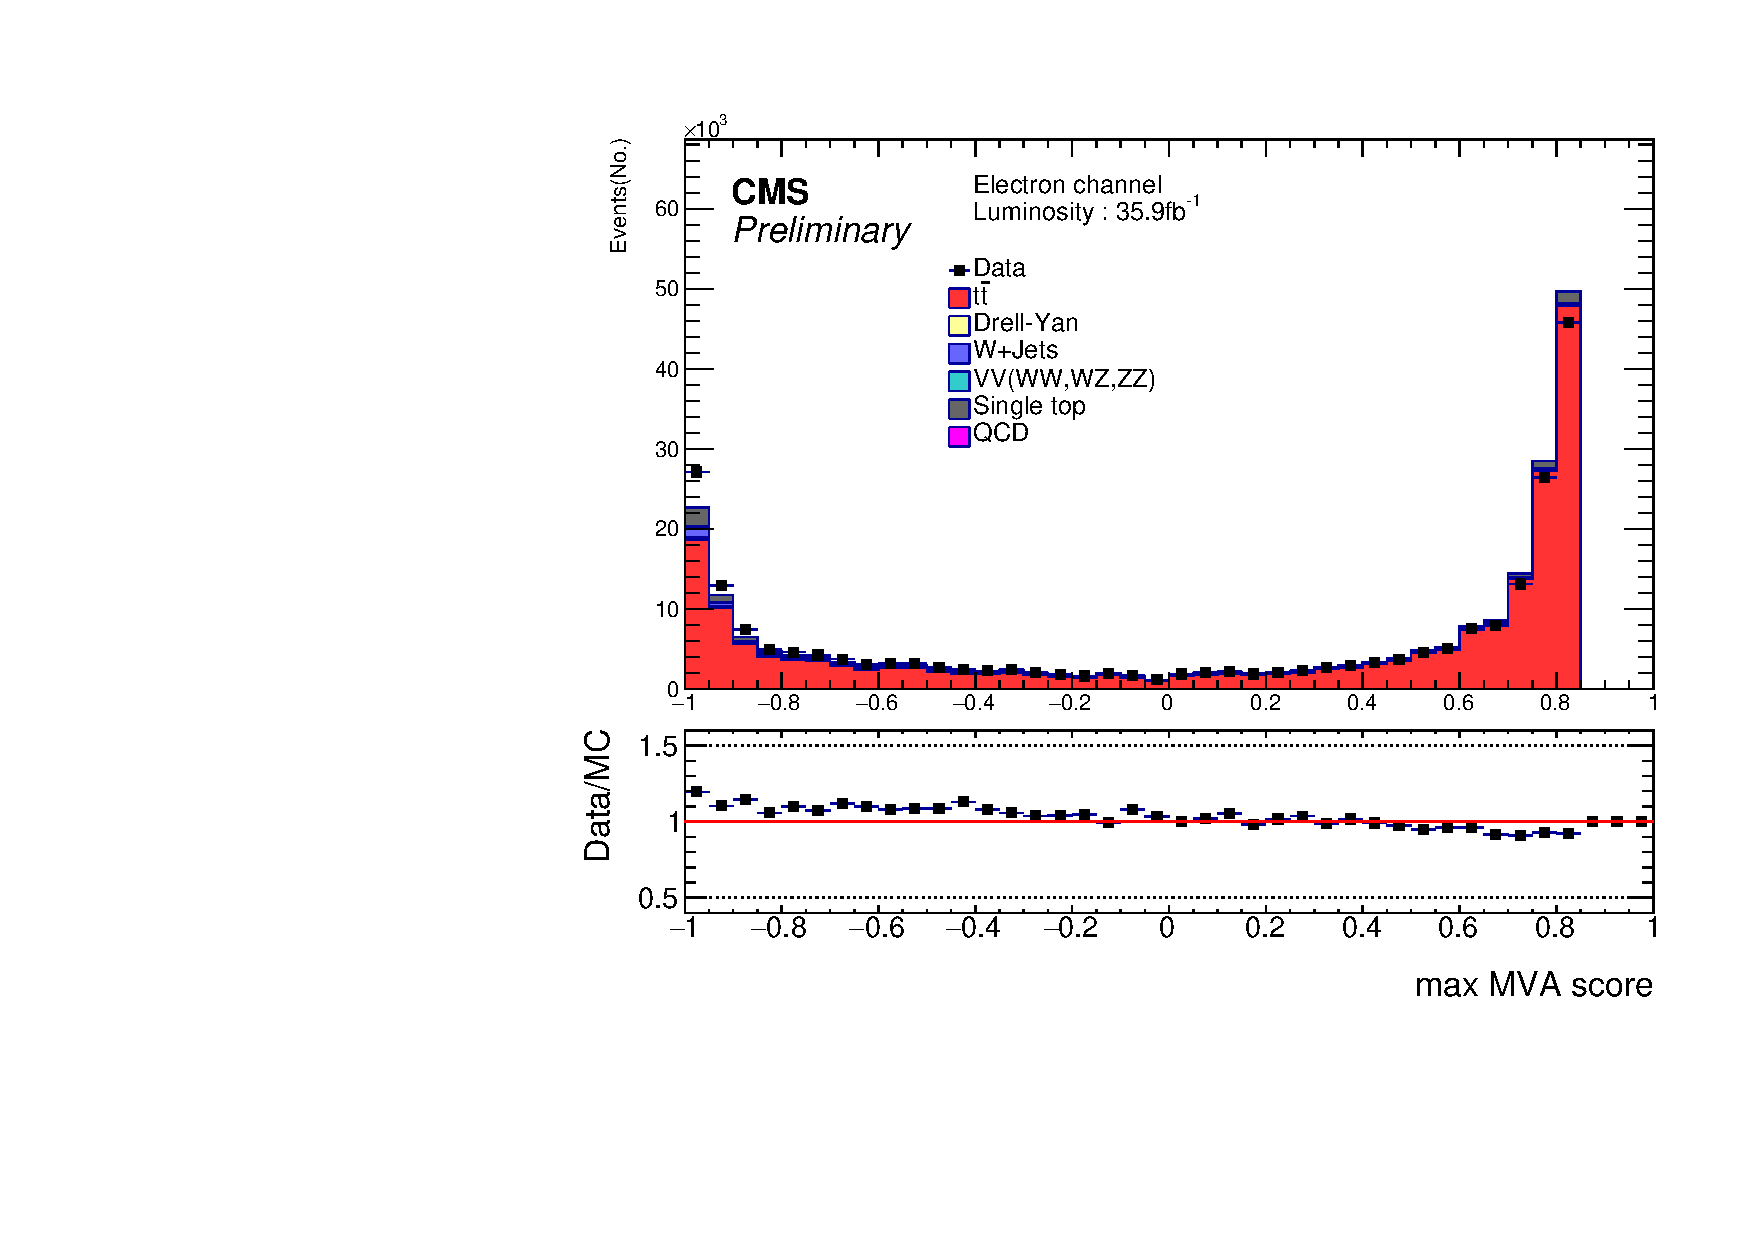
\includegraphics[width=0.32\textwidth]{Figures/EventSelReco/mva_algo/a04_BDTG_SR_algo_el.pdf}}
			    \subfigure[MLP (2 vars, el-ch)]{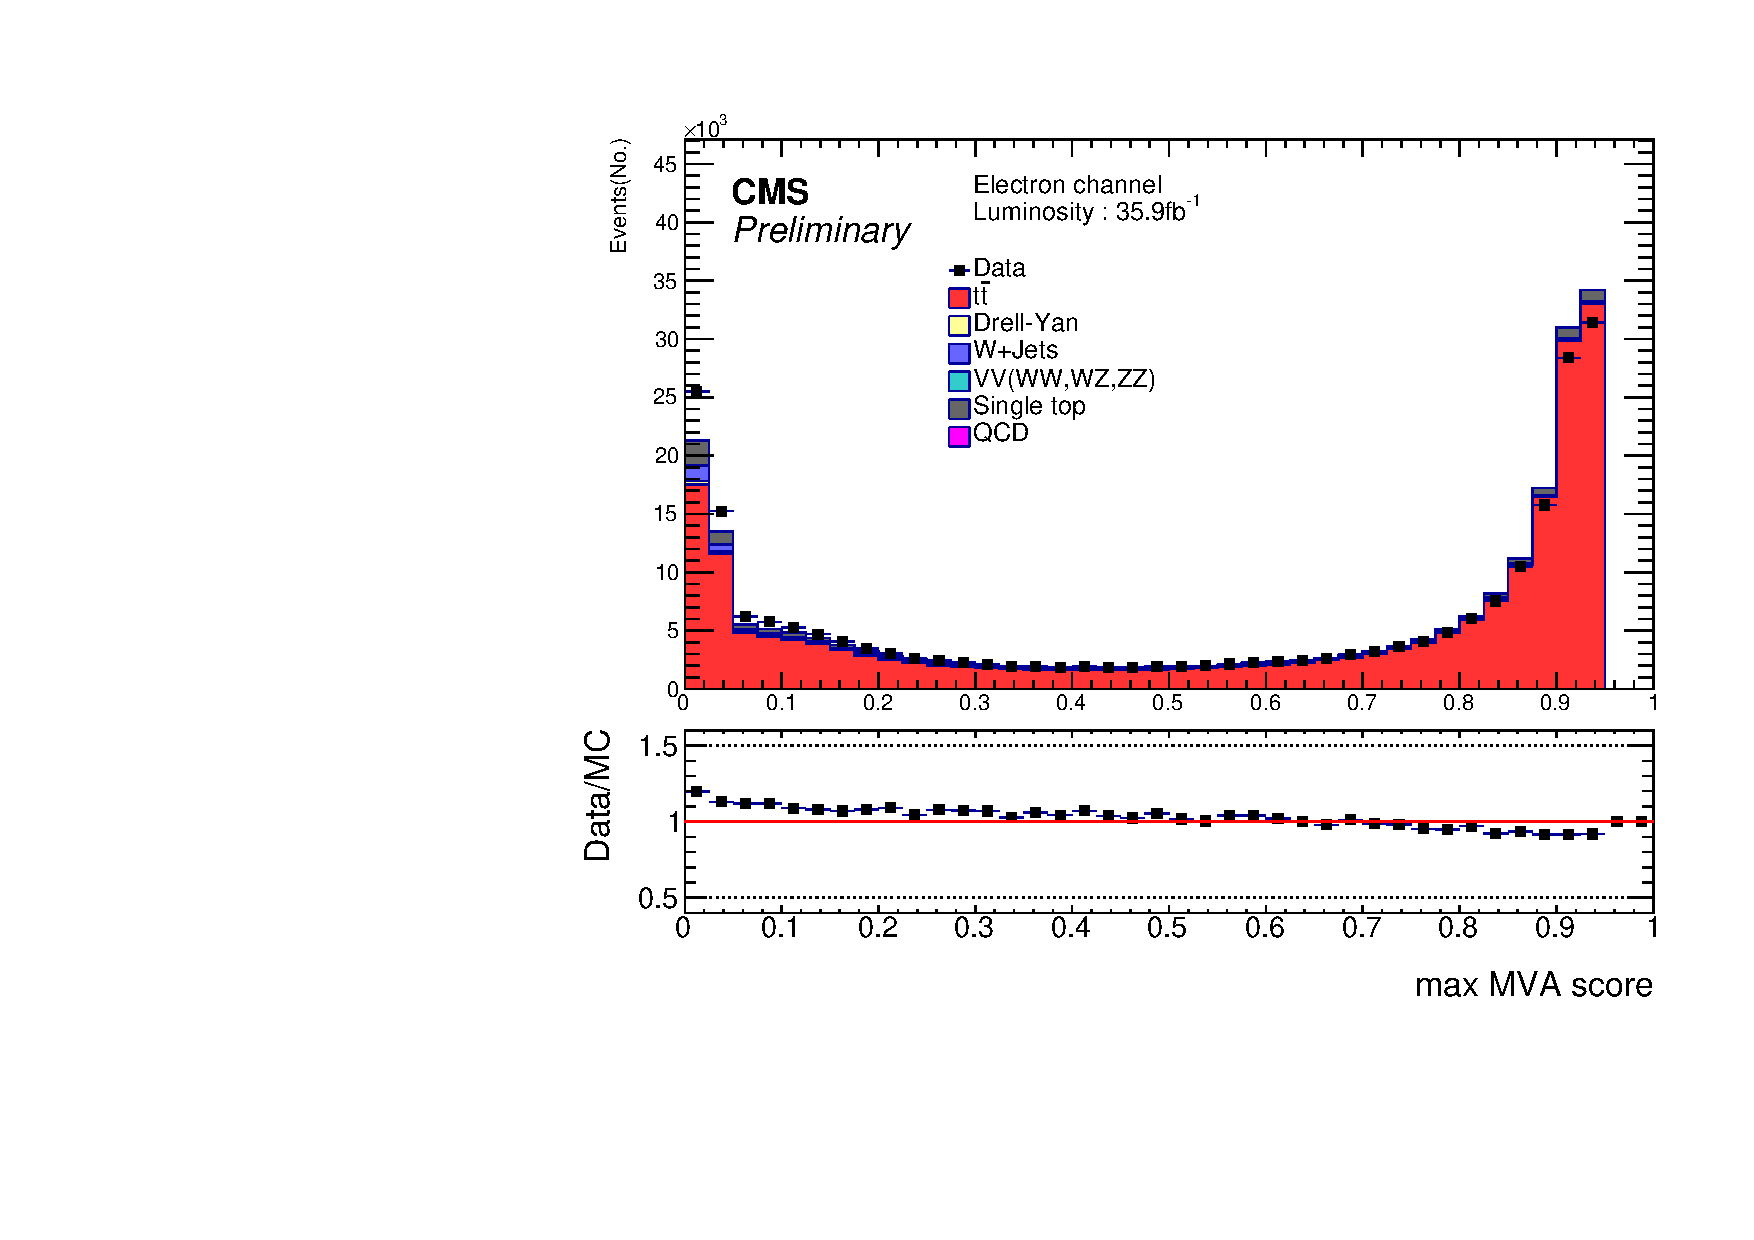
\includegraphics[width=0.32\textwidth]{Figures/EventSelReco/mva_algo/a04_MLP_SR_algo_el.pdf}}\\
			\caption{max MVA score in each event, comparing Data and MC.(2 variables training)}
			\label{EventSelReco:fig:a04_algo_DataMC}
			\end{figure}
			\FloatBarrier

			\begin{figure}[H]
			\centering
				\subfigure[BDT (8 vars, mu-ch)]{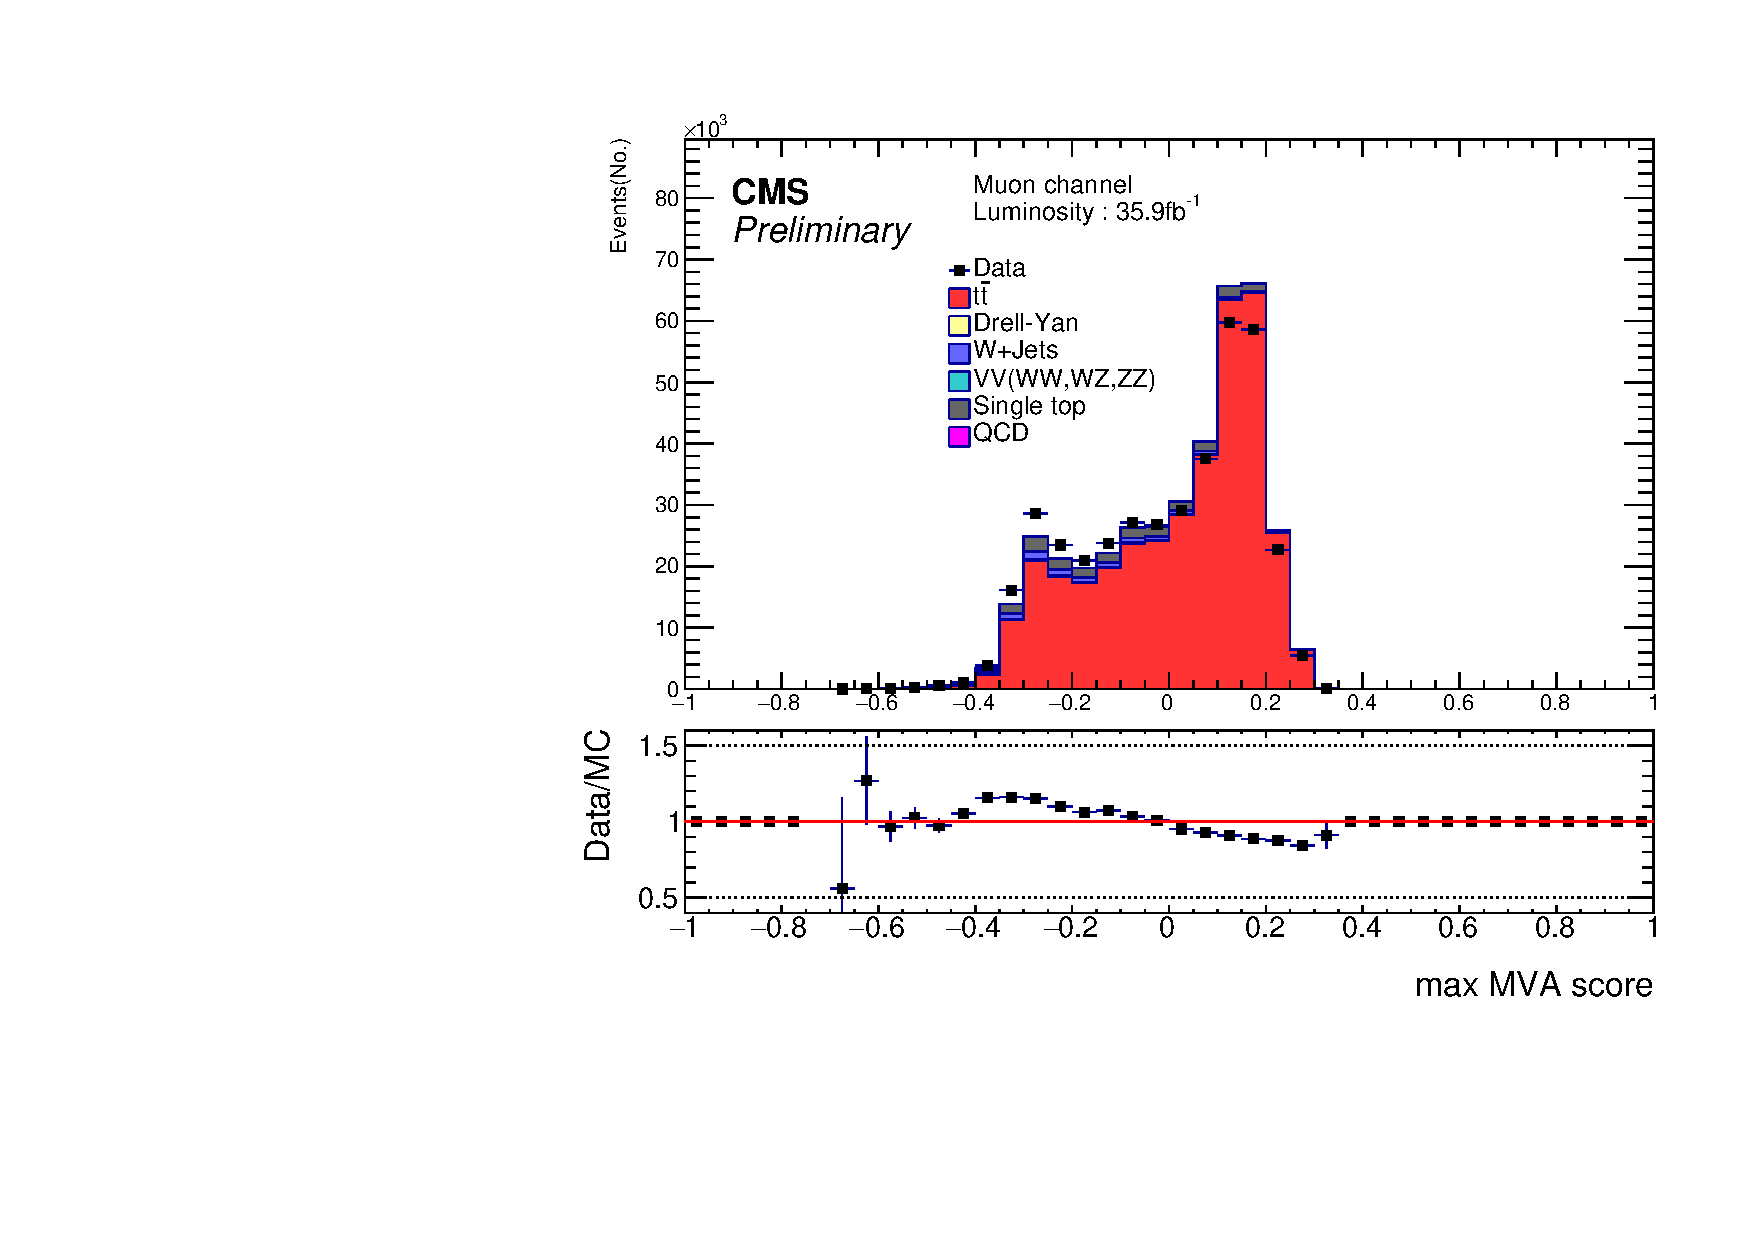
\includegraphics[width=0.32\textwidth]{Figures/EventSelReco/mva_algo/t13_BDT_SR_algo_mu.pdf}}
			    \subfigure[BDTG (8 vars, mu-ch)]{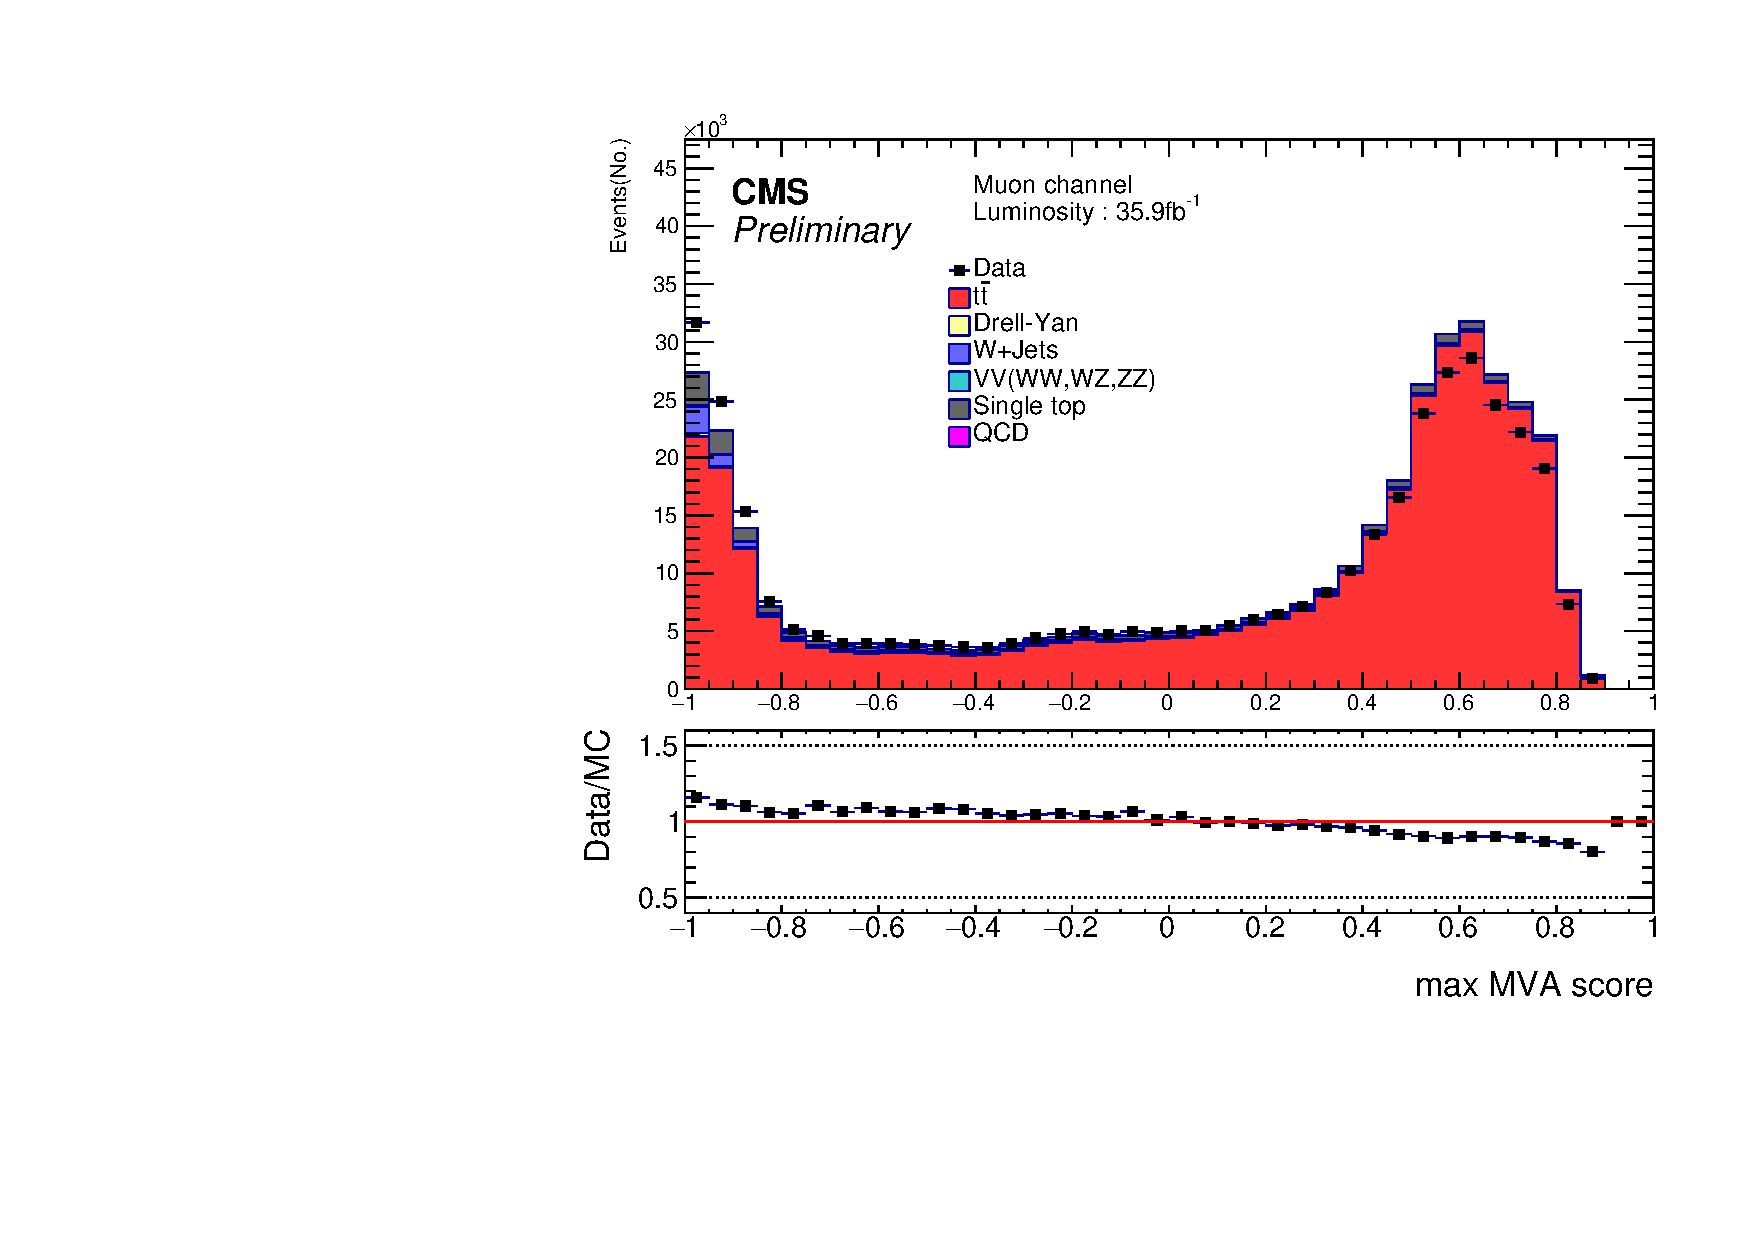
\includegraphics[width=0.32\textwidth]{Figures/EventSelReco/mva_algo/t13_BDTG_SR_algo_mu.pdf}}
			    \subfigure[MLP (8 vars, mu-ch)]{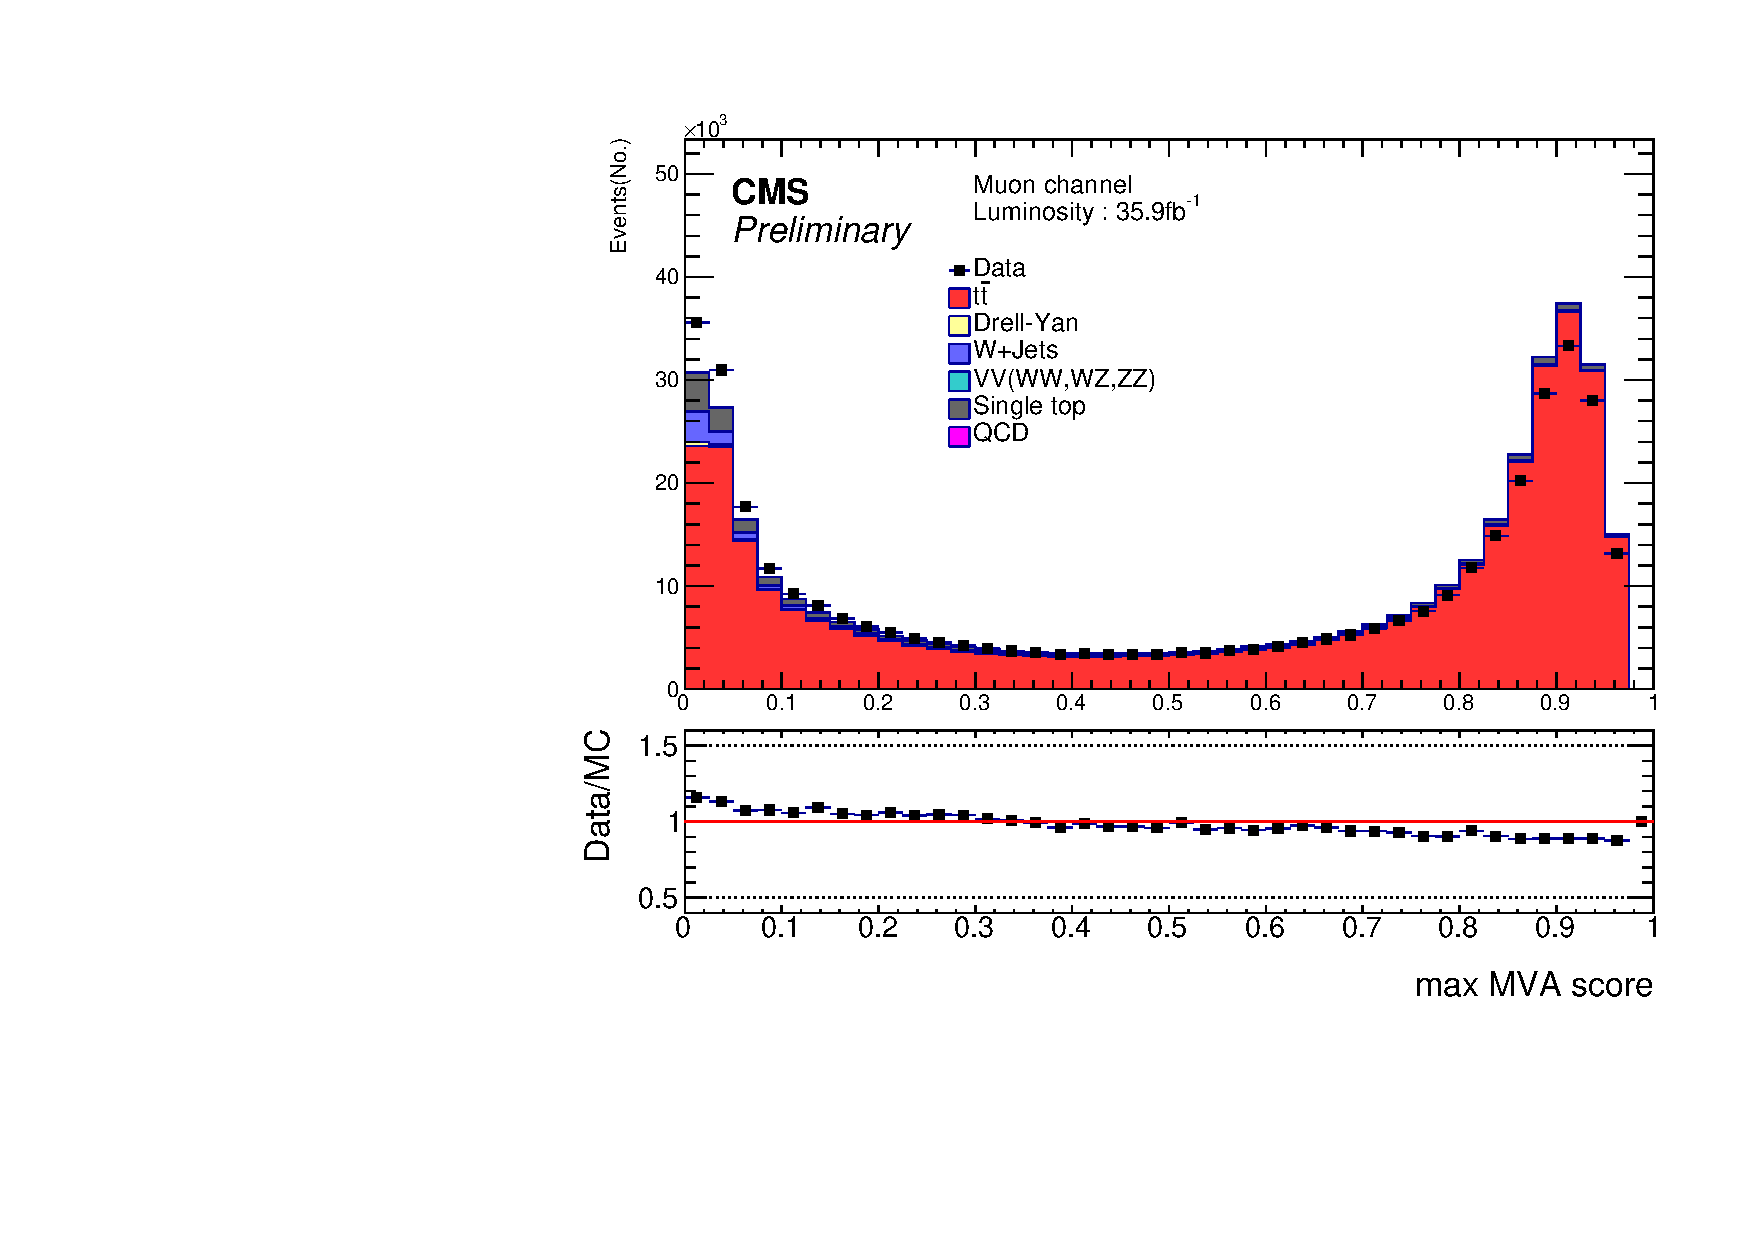
\includegraphics[width=0.32\textwidth]{Figures/EventSelReco/mva_algo/t13_MLP_SR_algo_mu.pdf}}\\			
			\end{figure}
			\FloatBarrier
			\begin{figure}[H]
			\centering
			    \subfigure[BDT (8 vars, el-ch)]{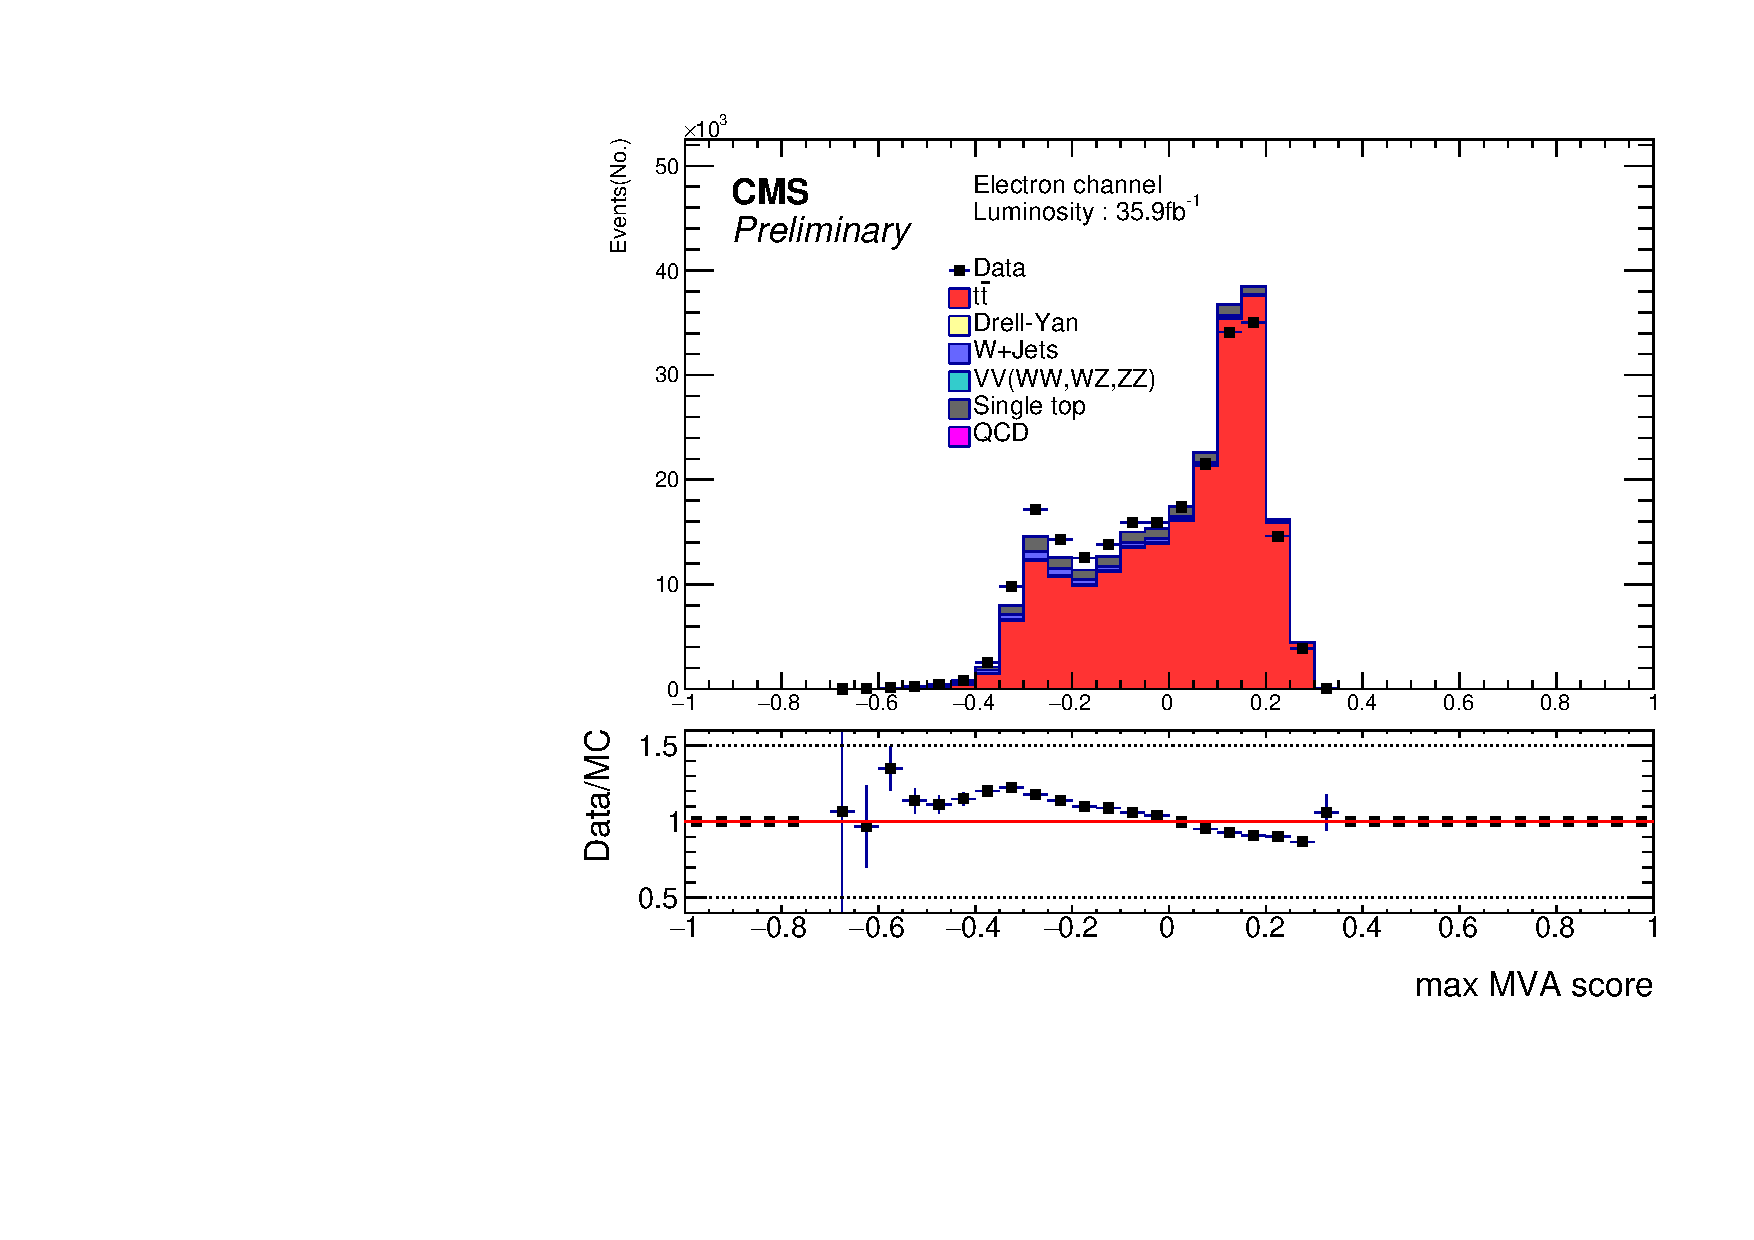
\includegraphics[width=0.32\textwidth]{Figures/EventSelReco/mva_algo/t13_BDT_SR_algo_el.pdf}}
			    \subfigure[BDTG (8 vars, el-ch)]{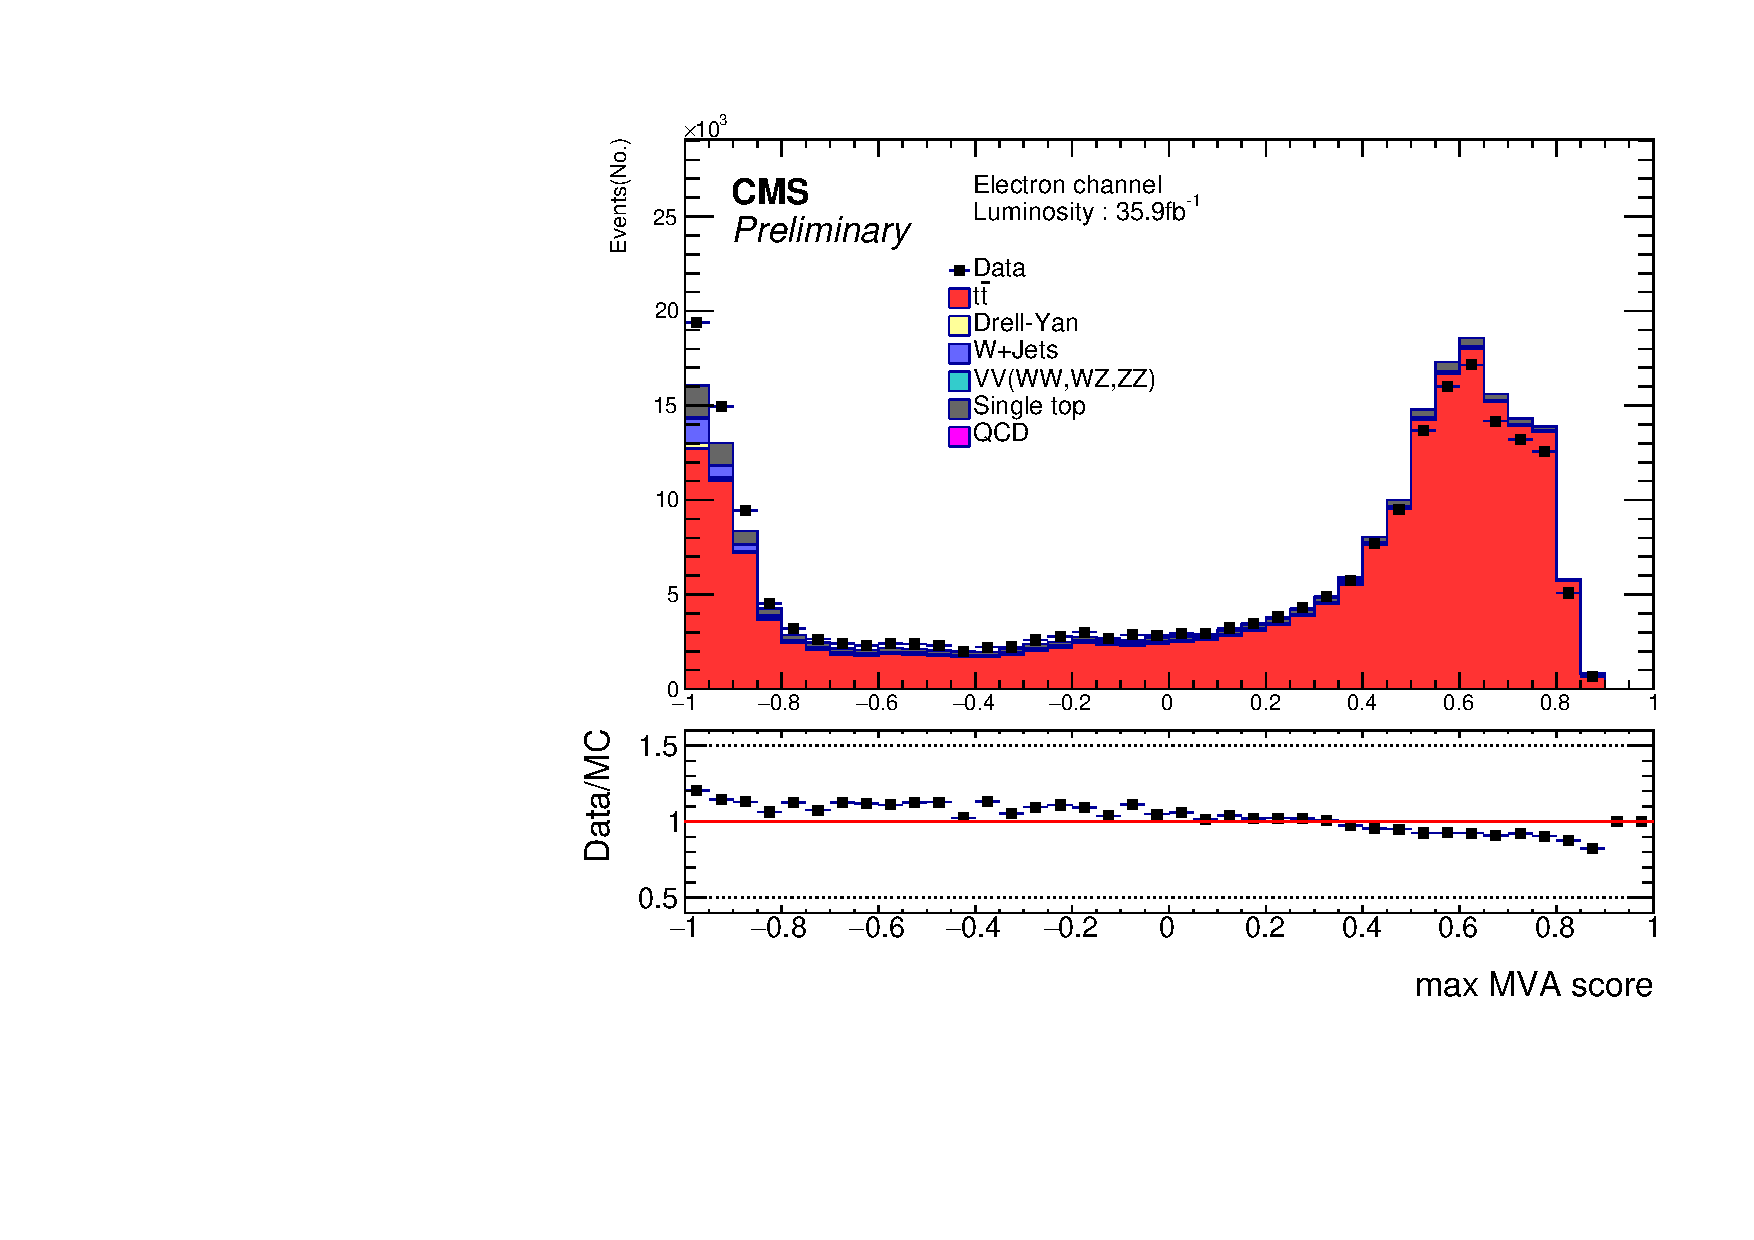
\includegraphics[width=0.32\textwidth]{Figures/EventSelReco/mva_algo/t13_BDTG_SR_algo_el.pdf}}
			    \subfigure[MLP (8 vars, el-ch)]{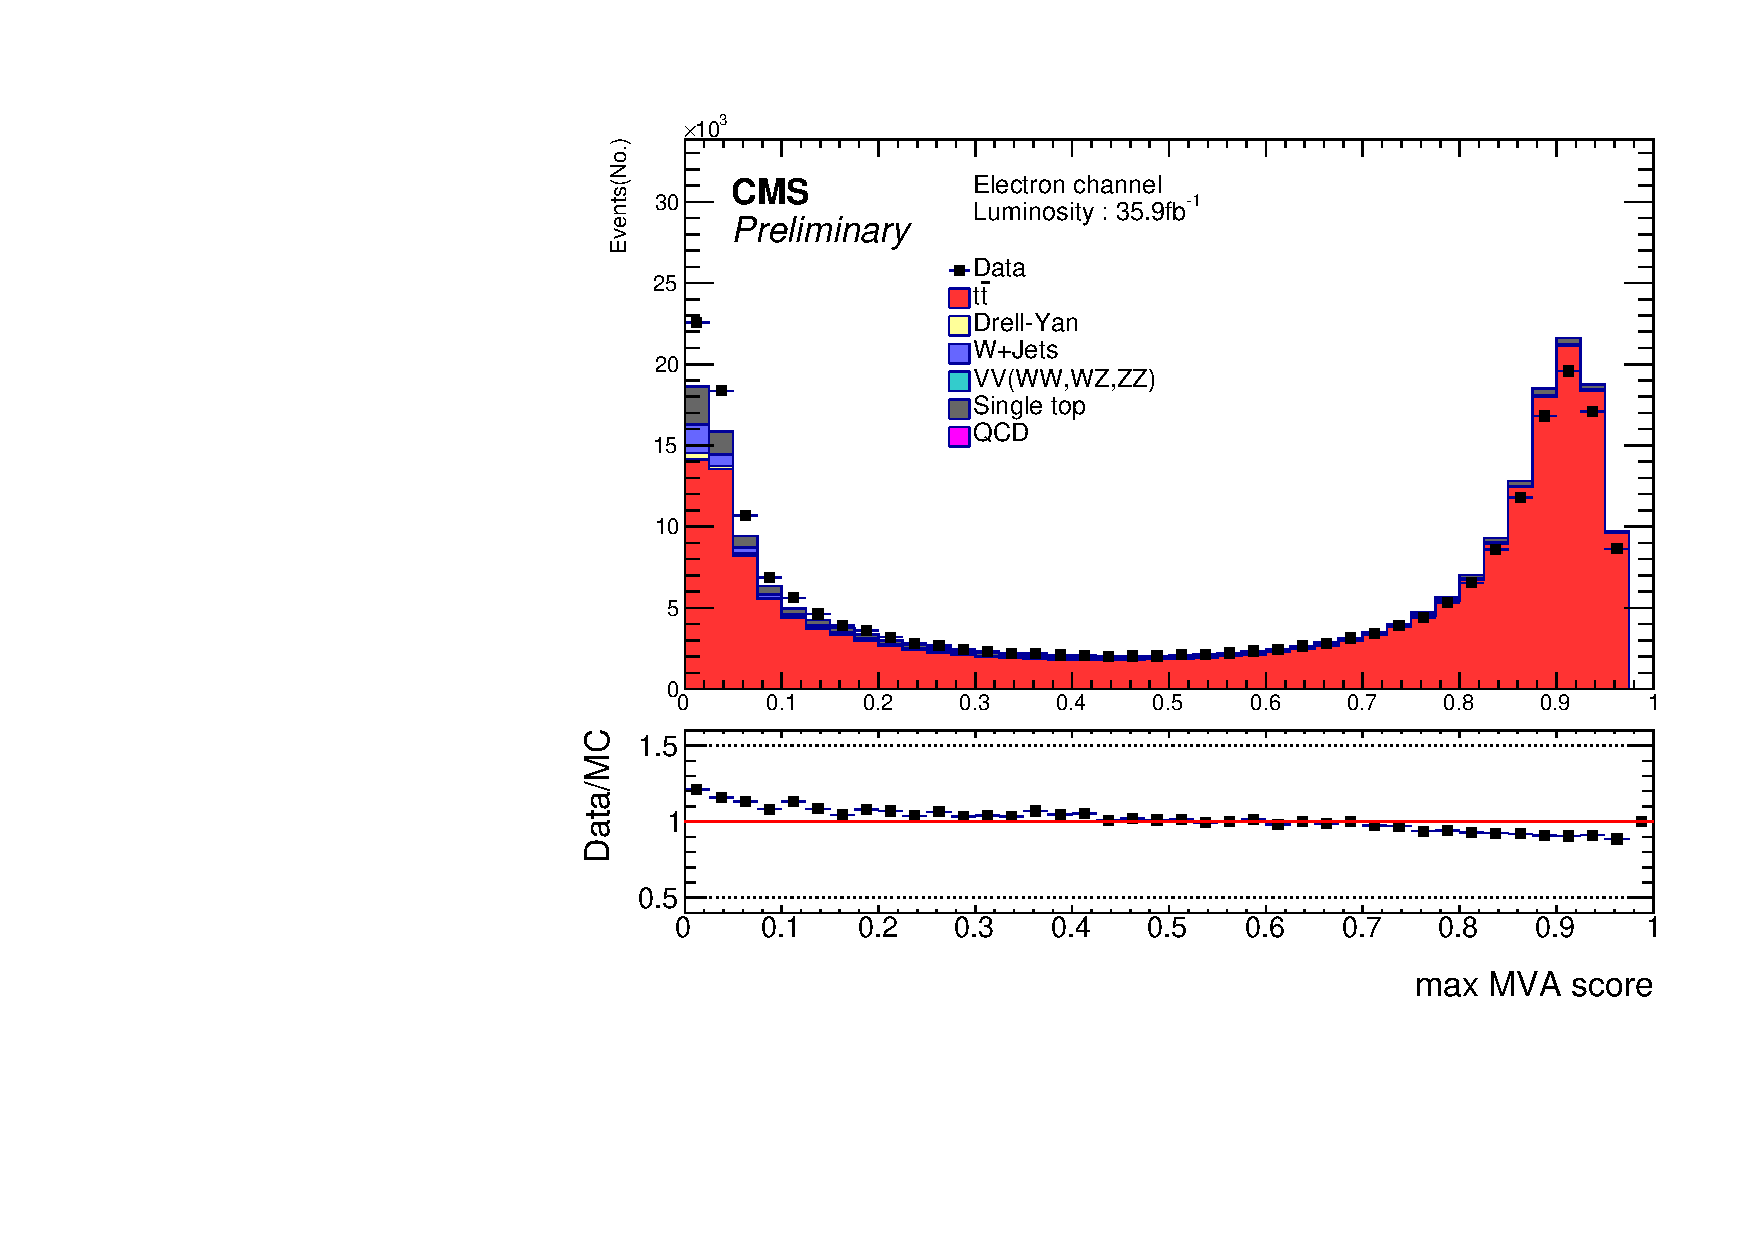
\includegraphics[width=0.32\textwidth]{Figures/EventSelReco/mva_algo/t13_MLP_SR_algo_el.pdf}}\\
			\caption{max MVA score in each event, comparing Data and MC.(8 variables training)}
			\label{EventSelReco:fig:t13_algo_DataMC}
			\end{figure}
			\FloatBarrier

			\begin{figure}[H]
			\centering
				\subfigure[BDT (20 vars, mu-ch)]{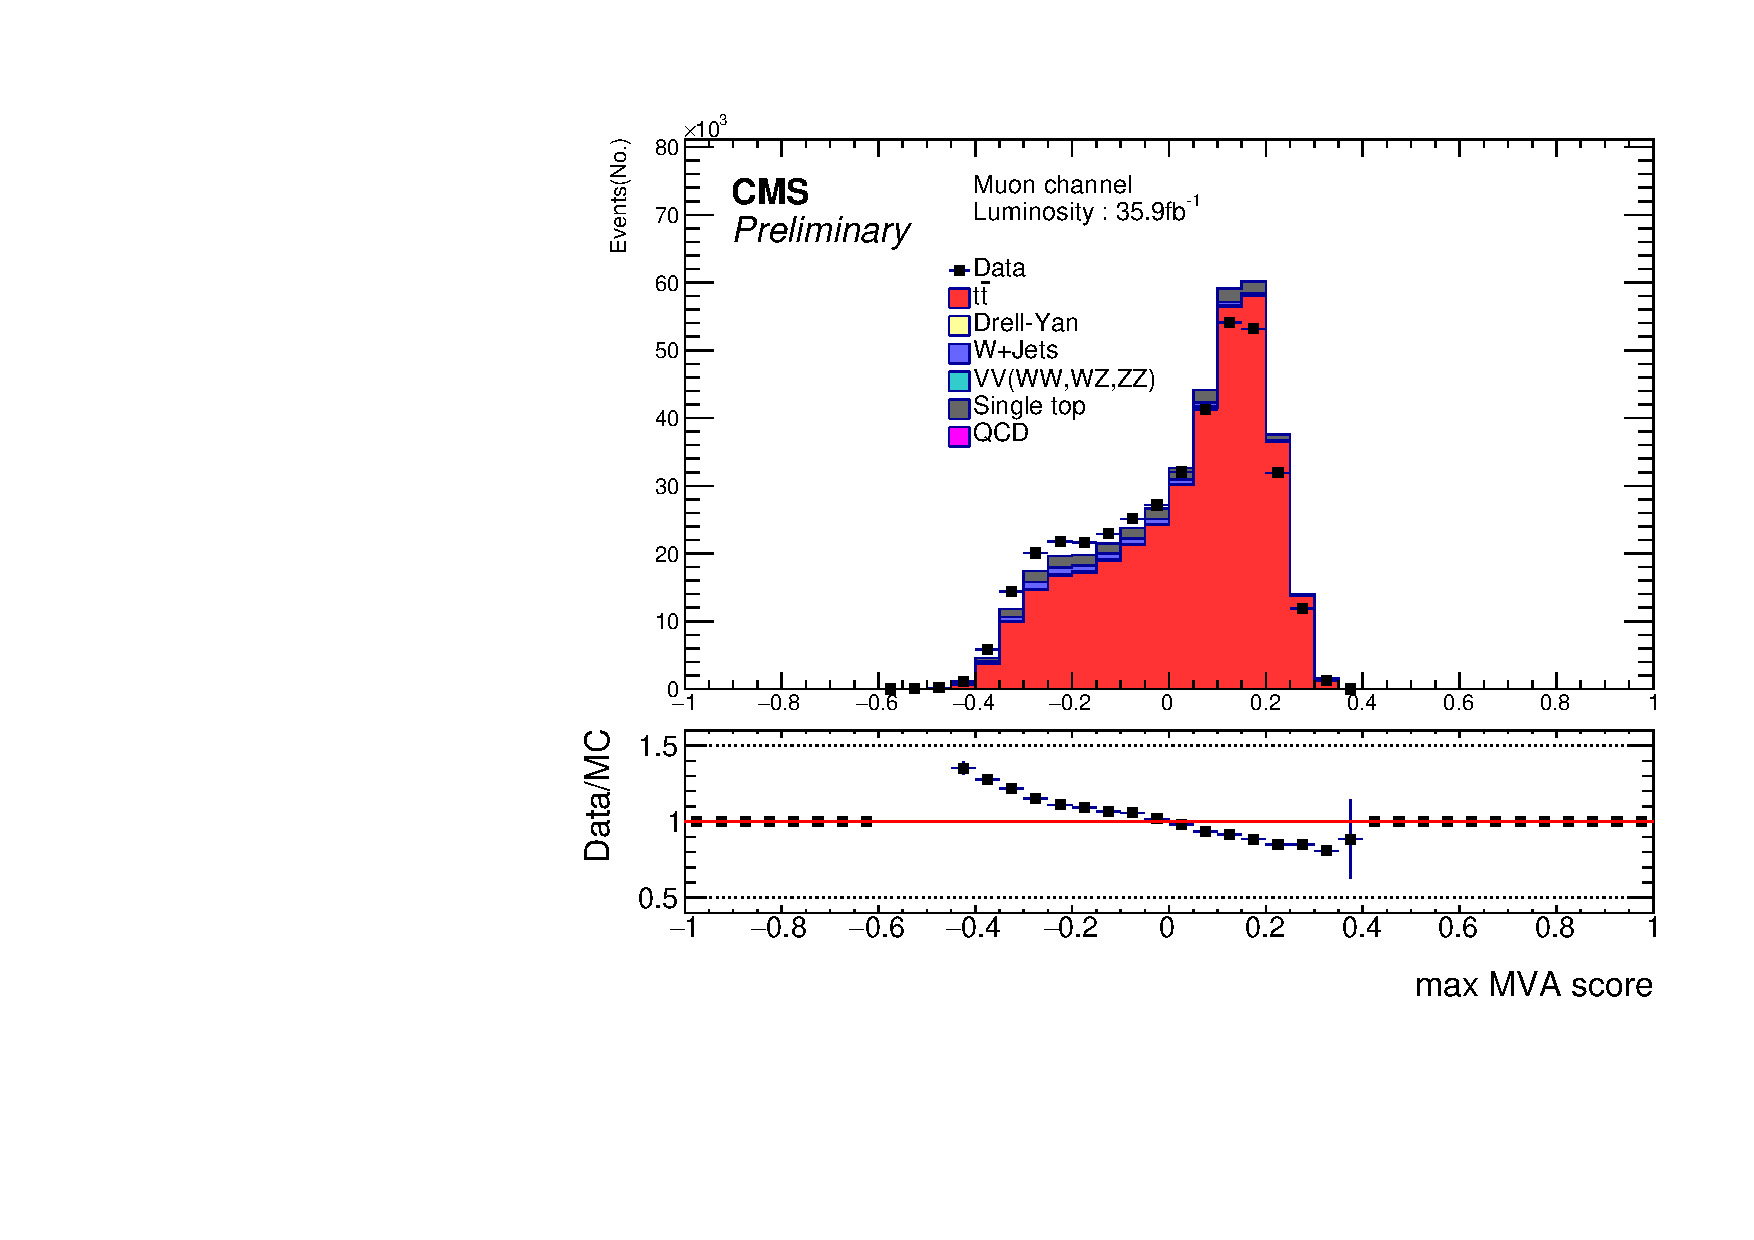
\includegraphics[width=0.32\textwidth]{Figures/EventSelReco/mva_algo/a05_BDT_SR_algo_mu.pdf}}
			    \subfigure[BDTG (20 vars, mu-ch)]{\includegraphics[width=0.32\textwidth]{Figures/EventSelReco/mva_algo/a05_BDTG_SR_algo_mu.pdf}}
			    \subfigure[MLP (20 vars, mu-ch)]{\includegraphics[width=0.32\textwidth]{Figures/EventSelReco/mva_algo/a05_MLP_SR_algo_mu.pdf}}\\
			\end{figure}
			\FloatBarrier
			\begin{figure}[H]
			\centering
			    \subfigure[BDT (20 vars, el-ch)]{\includegraphics[width=0.32\textwidth]{Figures/EventSelReco/mva_algo/a05_BDT_SR_algo_el.pdf}}
			    \subfigure[BDTG (20 vars, el-ch)]{\includegraphics[width=0.32\textwidth]{Figures/EventSelReco/mva_algo/a05_BDTG_SR_algo_el.pdf}}
			    \subfigure[MLP (20 vars, el-ch)]{\includegraphics[width=0.32\textwidth]{Figures/EventSelReco/mva_algo/a05_MLP_SR_algo_el.pdf}}\\
			\caption{max MVA score in each event, comparing Data and MC.(20 variables training)}
			\label{EventSelReco:fig:a05_algo_DataMC}
			\end{figure}
			\FloatBarrier

			%%% In the Fig.\ref{EventSelReco:fig:a04_algo_DataMC_mu} $\sim$ Fig.\ref{EventSelReco:fig:a05_algo_DataMC_el}, we can see that at the low and high max MVA score region, there is a little discrecpancy. It probably comes from the jet characteristic of jets multiplicity between Data and MC. In real data, there would be more soft jets than simulation(MC) sample. On the basis of number of jets, there are more probable combinations of jjb in data. It means that the max MVA value is more probable at low value in data. That is a possibility of the discrepancy.

			The training variables may have correlation with each other. If there are too much characteristic to be trained alike between variables, the most of input informations would duplicate. To check the variables' correlation score is necessary: (20 variables' case is shown)

			\begin{figure}[H]
			\centering
			    \subfigure[Variables in signal]{\includegraphics[width=0.45\textwidth]{Figures/EventSelReco/mva/a05_sig_cor.pdf}}
			    \subfigure[Variables in background]{\includegraphics[width=0.45\textwidth]{Figures/EventSelReco/mva/a05_bkg_cor.pdf}}\\
			\caption{Variables correlation with each other}
			\label{EventSelReco:fig:a05_correlation}
			\end{figure}
			\FloatBarrier

			No excess of correlation appear in training variables. The training variables would be also validated match between Data and MC:(20 variables MLP, muon channel is shown)

			\begin{figure}[H]
			\centering
			    \subfigure{\includegraphics[width=0.32\textwidth]{Figures/EventSelReco/mva_vars/VarCheck_j1j2_delR_NC_mu.pdf}}
			    \subfigure{\includegraphics[width=0.32\textwidth]{Figures/EventSelReco/mva_vars/VarCheck_j1j2_absdelPt_NC_mu.pdf}}
			    \subfigure{\includegraphics[width=0.32\textwidth]{Figures/EventSelReco/mva_vars/VarCheck_j1j2_sumPt_NC_mu.pdf}}\\
			\end{figure}
			\FloatBarrier

			\begin{figure}[H]
			\centering
			    \subfigure{\includegraphics[width=0.32\textwidth]{Figures/EventSelReco/mva_vars/VarCheck_whadb_delR_NC_mu.pdf}}
			    \subfigure{\includegraphics[width=0.32\textwidth]{Figures/EventSelReco/mva_vars/VarCheck_whadb_delPt_NC_mu.pdf}}
			    \subfigure{\includegraphics[width=0.32\textwidth]{Figures/EventSelReco/mva_vars/VarCheck_whadb_sumPt_NC_mu.pdf}}\\
			\end{figure}
			\FloatBarrier

			\begin{figure}[H]
			\centering
			    \subfigure{\includegraphics[width=0.32\textwidth]{Figures/EventSelReco/mva_vars/VarCheck_hadblepton_delR_NC_mu.pdf}}
			    \subfigure{\includegraphics[width=0.32\textwidth]{Figures/EventSelReco/mva_vars/VarCheck_hadblepton_delPt_NC_mu.pdf}}
			    \subfigure{\includegraphics[width=0.32\textwidth]{Figures/EventSelReco/mva_vars/VarCheck_hadblepton_sumPt_NC_mu.pdf}}\\
			\end{figure}
			\FloatBarrier

			\begin{figure}[H]
			\centering
			    \subfigure{\includegraphics[width=0.32\textwidth]{Figures/EventSelReco/mva_vars/VarCheck_hadwlepton_delR_NC_mu.pdf}}
			    \subfigure{\includegraphics[width=0.32\textwidth]{Figures/EventSelReco/mva_vars/VarCheck_hadwlepton_delPt_NC_mu.pdf}}
			    \subfigure{\includegraphics[width=0.32\textwidth]{Figures/EventSelReco/mva_vars/VarCheck_hadwlepton_sumPt_NC_mu.pdf}}\\
			\end{figure}
			\FloatBarrier

			\begin{figure}[H]
			\centering
			    \subfigure{\includegraphics[width=0.32\textwidth]{Figures/EventSelReco/mva_vars/VarCheck_hadwmet_delPhi_NC_mu.pdf}}
			    \subfigure{\includegraphics[width=0.32\textwidth]{Figures/EventSelReco/mva_vars/VarCheck_hadwmet_delPt_NC_mu.pdf}}
			    \subfigure{\includegraphics[width=0.32\textwidth]{Figures/EventSelReco/mva_vars/VarCheck_hadwmet_sumPt_NC_mu.pdf}}\\
			\end{figure}
			\FloatBarrier

			\begin{figure}[H]
			\centering
			    \subfigure{\includegraphics[width=0.32\textwidth]{Figures/EventSelReco/mva_vars/VarCheck_hadbmet_delPhi_NC_mu.pdf}}
			    \subfigure{\includegraphics[width=0.32\textwidth]{Figures/EventSelReco/mva_vars/VarCheck_hadbmet_delPt_NC_mu.pdf}}
			    \subfigure{\includegraphics[width=0.32\textwidth]{Figures/EventSelReco/mva_vars/VarCheck_hadbmet_sumPt_NC_mu.pdf}}\\
			\end{figure}
			\FloatBarrier

			\begin{figure}[H]
			\centering
			    \subfigure{\includegraphics[width=0.45\textwidth]{Figures/EventSelReco/mva_vars/VarCheck_mjj_NC_mu.pdf}}
			    \subfigure{\includegraphics[width=0.45\textwidth]{Figures/EventSelReco/Mass/a05/a05_MLP_NC_long_HadTop_mu.pdf}}\\
			\label{EventSelReco:fig:a05_DataMC_vars}
			\caption{20 variables' Data/MC comparison(MLP, mu-ch)}
			\end{figure}
			\FloatBarrier

	\subsection{$b\bar{b}$ separation and distinguishment}
	\label{ssec:bbsep}

		The good correctness of chosen physical objects is necessary in this analysis. By the basis for discovering new physics, the observables require precise identification of particles. And the important is, in our selected observables, to distinguish $b$- between $\bar{b}$ -quark which are both b-tagged jets detected from smashing and hadronizatoin of b-flavor quarks. For example, the identification is highly correlated with observable $O_{6}$ which is $q_{l}(\vec{p_{b}}-\vec{p_{\bar{b}}})\cdot(\vec{p_{l}}\times\vec{p_{j_{1}}})$, the mis-ordered $b$/($\bar{b}$) will cause the wrong sign on this observable. On the other hand, it is not requirement for us to correctly pick up the 2 jets from hadronic top quark in this analysis. Also, the long tail in reconstructed hadronic top invariant mass($M_{jjb}$, Fig.\ref{EventSelReco:fig:a04_MLP_SR_NC_Mjjb}, Fig.\ref{EventSelReco:fig:t13_MLP_SR_NC_Mjjb}, Fig.\ref{EventSelReco:fig:a05_MLP_SR_NC_Mjjb}) deviated too much from known top mass 172.5GeV. And the source of this tail is infered coming from $b/\bar{b}$ wrong identified cases. In this way, the identification between $b$ and $\bar{b}$ is the most critical implication. And that is also what we need to test the performance of reconstruction algorithm($\chi^2_{min}$,MVA). 

		All the following study in \ref{ssec:bbsep} is worked only under the signal simulation sample($t$$\bar{t}$ Monte Carlo). All the selected physical objects include jets and leptons will be matched to particle with the generator-level information in MC sample with $\Delta R$ < 0.4 method.(Eq.\ref{eq:gen_matching})

		To standardlize the $b$/$\bar{b}$ distinguishment, there are 3 classifications listed:
		\begin{itemize}
  		\item $\textbf{Correct}$: $b$-quark is identified as $b$-jets and $\bar{b}$-quark is identified as $\bar{b}$-jets
  		\item $\textbf{b/}$$\bar{\textbf{b}}$ $\textbf{mis-identified}$: $b$-quark is identified as $\bar{b}$-jets and $\bar{b}$-quark is identified as $b$-jets
  		\item $\textbf{Mistag}$: non $b$$(\bar{b})$-quark is identified as $b$$(\bar{b})$-jet
		\end{itemize}

		With applying the various algorithm on signal simulation sample($t\bar{t}$ MC), there are the $b/\bar{b}$-distinguishment results after reconstructed the hadronic top and make a identification of physical objects via $\chi^2_{min}$ and MVA methods:

		\begin{center}
		\begin{longtable}[H]{ c c | c c c }			% add the [H] can make it listed in table list!!
		\caption{$b/\bar{b}$ disdinguishment under different algorithm (w/o cut)}\\
		\hline
		[\%] & & Correct & $b\bar{b}$ mis-identified & Mistag  \\ 
		\hline
		$\chi^2_{min}$ &  & 61.18 & 25.21 & 13.38 \\
		\hline
		\multirow{3}{5em}{2 variables} & MLP & 63.18 & 23.22 & 13.60 \\
		& BDT & 60.89 & 25.49 & 13.60 \\
		& BDTG & 63.02 & 23.37 & 13.61 \\
		\hline
		\multirow{3}{5em}{8 variables} & MLP & 72.36 & 14.02 & 13.62 \\
		& BDT & 72.02 & 14.37 & 13.60 \\
		& BDTG & 71.00 & 15.39 & 13.61 \\
		\hline
		\multirow{3}{5em}{20 variables} & MLP & 71.27 & 15.13 & 13.61 \\
		& BDT & 71.07 & 15.32 & 13.61 \\
		& BDTG & 69.59 & 16.79 & 13.61 \\
		\hline
		\label{EventSelReco:tb:nocut_bbsep}
		\end{longtable}
		\end{center}

		This is shown that the MLP algorithm have the best performance under these 3 training variables sets. As our expected, the 2 variables training result is close to $\chi^2_{min}$ method's because of their same variables input to be deduced. And the 8 variables set and 20 variables set are both good at discreminate $b/\bar{b}$, which can lead us to choose these to be optimized one. It is also known that $\emph{Mistag}$'s ratio in Table.\ref{EventSelReco:tb:nocut_bbsep} are almost the same since it is primarily pre-decided by the b-tagged selection.

		In addition to applying algorithm to reconstruct $M_{jjb}$ and identify the physical objects, there are also some optimization cut done on this step. In the concept of $\chi^2_{min}$ method, the smaller the $\chi^2$ value(Eq.\ref{eq:chi2}), the less possibility that this combination is the one we want. So we can apply cut on $\chi^2$ value. If in an event the chosen combination whose $\chi^2_{min}$ is still bigger than the cut, the event will be threw away. These thrown away events are identified as the events which come from the mis-tag objects from detector or some events come from other physics decay(background) not $t\bar{t}$. The most important is that, it can cut out the events which are not $b/\bar{b}$-correct distinguished. So the cut is set to be at $\chi^2_{min}$ < 20, and to standardize the optimization, there are also use the $b/\bar{b}$ distinguishment results to see the performance.

		There is the cross-check plot(Fig.\ref{EventSelReco:fig:chi2_2D}) which shows that the high $\chi^2$ value correspond to the $m_{jjb}$ distant from the expected $m_{jjb}$ in Eq.\ref{eq:chi2}.

		\begin{figure}[H]
		\centering{}
    		\includegraphics[width=0.65\textwidth]{Figures/EventSelReco/bbsep/chi2_2D.pdf}\\
		\caption{$\chi^2_{min}$-reco $m_{jjb}$}
		\label{EventSelReco:fig:chi2_2D}
		\end{figure}
		\FloatBarrier

		To check that the cut on the $\chi^2_{min}$ really rule out incorrect $b/\bar{b}$-identified more effeciently than correct case. This plot(Fig.\ref{EventSelReco:fig:chi2_bbsep_pdf}) shows that the incorrect cases(exchange-identified and mistag) do have more ratio at the higher $\chi^2_{min}$ score than the correct case. It make the $\chi^2_{min}$ cut more persuasive.

		\begin{figure}[H]
		\centering
		    \includegraphics[width=0.65\textwidth]{Figures/EventSelReco/bbsep/chi2_bbsep.pdf}\\
		\caption{$b/\bar{b}$ identified result related to $\chi^2_{min}$(pdf)}
		\label{EventSelReco:fig:chi2_bbsep_pdf}
		\end{figure}
		\FloatBarrier

		There is the result that if we cut on the $\chi^2_{min}$ value and how the 3 $b/\bar{b}$-identified classifications' ratios vary. It is also shown that the events efficiency which is the ratio of events survived under this optimized cut.

		\begin{figure}[H]
		\centering
		    \includegraphics[width=0.65\textwidth]{Figures/EventSelReco/bbsep/chi2_eff_t.pdf}\\ 
		\caption{cut on $\chi^2_{min}$ and ratio of 3 classification}
		\label{EventSelReco:fig:chi2_bbsep_eff}
		\end{figure}
		\FloatBarrier

		\begin{center}
		\begin{longtable}[H]{ c c | c c c }
		\caption{$b/\bar{b}$ disdinguishment under $\chi^2_{min}$ method (w/ $\chi^2_{min}$ < 20 cut)}\\
		\hline
		[\%] & Channel & Correct & $b\bar{b}$ mis-identified & Mistag  \\ 
		\hline{}
		\multirow{2}{2em}{$\chi^2_{min}$} & Electron Channel & 65.47 & 22.29 & 12.24 \\
		& Muon Channel & 65.65 & 22.29 & 12.06 \\
		\hline
		\label{EventSelReco:tb:chi2_algocut_bbsep}
		\end{longtable}
		\end{center}

		And as same concept as the optimized cut on $\chi^2_{min}$ value in $\chi^2_{min}$ method, there would be also optimization cut applied on MVA method. In comparison with that low $\chi^2$ value is better choice, combination with high MVA score is the better one in MVA method. It also can have a cut on MVA score to subtract incorrect $b/\bar{b}$-identified selection. Same scenario as $\chi^2_{min}$ method, if in an event the maximum MVA score(which belongs to the chosen combination) is still lower than the cut, the event will be threw away. We still need to check the relation between MVA score and $M_{jjb}$, and also check the ratio of 3 $b/\bar{b}$-classifications that the incorrect cases has more ratio at lower MVA score. There are the plots of 2 variables/8 variables/20 variables sets with MLP/BDT/BDTG training method:

		\begin{figure}[H]
		\centering
			\subfigure[BDT]{\includegraphics[width=0.32\textwidth]{Figures/EventSelReco/bbsep/a04_BDT_2D.pdf}}
			\subfigure[BDTG]{\includegraphics[width=0.32\textwidth]{Figures/EventSelReco/bbsep/a04_BDTG_2D.pdf}}
			\subfigure[MLP]{\includegraphics[width=0.32\textwidth]{Figures/EventSelReco/bbsep/a04_MLP_2D.pdf}}\\
			\subfigure[BDT]{\includegraphics[width=0.32\textwidth]{Figures/EventSelReco/bbsep/a04_BDT_bbsep3.pdf}}
			\subfigure[BDTG]{\includegraphics[width=0.32\textwidth]{Figures/EventSelReco/bbsep/a04_BDTG_bbsep3.pdf}}
		    \subfigure[MLP]{\includegraphics[width=0.32\textwidth]{Figures/EventSelReco/bbsep/a04_MLP_bbsep3.pdf}}\\
		\caption{MVA score-reco $m_{jjb}$ plots and $b/\bar{b}$ identified result related to MVA value (2 variables training)}
		\label{EventSelReco:fig:a04_bbsep}
		\end{figure}
		\FloatBarrier

		\begin{figure}[H]
		\centering
			\subfigure[BDT]{\includegraphics[width=0.32\textwidth]{Figures/EventSelReco/bbsep/t13_BDT_2D.pdf}}
			\subfigure[BDTG]{\includegraphics[width=0.32\textwidth]{Figures/EventSelReco/bbsep/t13_BDTG_2D.pdf}}
			\subfigure[MLP]{\includegraphics[width=0.32\textwidth]{Figures/EventSelReco/bbsep/t13_MLP_2D.pdf}}\\
			\subfigure[BDT]{\includegraphics[width=0.32\textwidth]{Figures/EventSelReco/bbsep/t13_BDT_bbsep3.pdf}}
			\subfigure[BDTG]{\includegraphics[width=0.32\textwidth]{Figures/EventSelReco/bbsep/t13_BDTG_bbsep3.pdf}}
		    \subfigure[MLP]{\includegraphics[width=0.32\textwidth]{Figures/EventSelReco/bbsep/t13_MLP_bbsep3.pdf}}\\
		\caption{MVA score-reco $m_{jjb}$ plots and $b/\bar{b}$ identified result related to MVA value (8 variables training)}
		\label{EventSelReco:fig:t13_bbsep}
		\end{figure}
		\FloatBarrier

		\begin{figure}[H]
		\centering
			\subfigure[BDT]{\includegraphics[width=0.32\textwidth]{Figures/EventSelReco/bbsep/a05_BDT_2D.pdf}}
			\subfigure[BDTG]{\includegraphics[width=0.32\textwidth]{Figures/EventSelReco/bbsep/a05_BDTG_2D.pdf}}
			\subfigure[MLP]{\includegraphics[width=0.32\textwidth]{Figures/EventSelReco/bbsep/a05_MLP_2D.pdf}}\\
			\subfigure[BDT]{\includegraphics[width=0.32\textwidth]{Figures/EventSelReco/bbsep/a05_BDT_bbsep3.pdf}}
			\subfigure[BDTG]{\includegraphics[width=0.32\textwidth]{Figures/EventSelReco/bbsep/a05_BDTG_bbsep3.pdf}}			
		    \subfigure[MLP]{\includegraphics[width=0.32\textwidth]{Figures/EventSelReco/bbsep/a05_MLP_bbsep3.pdf}}\\
		\caption{MVA score-reco $m_{jjb}$ plots and $b/\bar{b}$ identified result related to MVA value (20 variables training)}
		\label{EventSelReco:fig:a05_bbsep}
		\end{figure}
		\FloatBarrier

		There are also the effeciency plots shows that if it's given a cut on MVA score, how these 3 $b/\bar{b}$-identified cases' ratio vary.

		\begin{figure}[H]
		\centering
			\subfigure[BDT]{\includegraphics[width=0.32\textwidth]{Figures/EventSelReco/bbsep/a04_BDT_eff_t.pdf}}
			\subfigure[BDTG]{\includegraphics[width=0.32\textwidth]{Figures/EventSelReco/bbsep/a04_BDTG_eff_t.pdf}}
			\subfigure[MLP]{\includegraphics[width=0.32\textwidth]{Figures/EventSelReco/bbsep/a04_MLP_eff_t.pdf}}\\
		\caption{cut on MVA score and ratio of 3 classification (2 variables training)}
		\label{EventSelReco:fig:a04_bbsep_eff}
		\end{figure}
		\FloatBarrier

		\begin{figure}[H]
		\centering
			\subfigure[BDT]{\includegraphics[width=0.32\textwidth]{Figures/EventSelReco/bbsep/t13_BDT_eff_t.pdf}}
			\subfigure[BDTG]{\includegraphics[width=0.32\textwidth]{Figures/EventSelReco/bbsep/t13_BDTG_eff_t.pdf}}
			\subfigure[MLP]{\includegraphics[width=0.32\textwidth]{Figures/EventSelReco/bbsep/t13_MLP_eff_t.pdf}}\\
		\caption{cut on MVA score and ratio of 3 classification (8 variables training)}
		\label{EventSelReco:fig:t13_bbsep_eff}
		\end{figure}
		\FloatBarrier

		\begin{figure}[H]
		\centering
			\subfigure[BDT]{\includegraphics[width=0.32\textwidth]{Figures/EventSelReco/bbsep/a05_BDT_eff_t.pdf}}
			\subfigure[BDTG]{\includegraphics[width=0.32\textwidth]{Figures/EventSelReco/bbsep/a05_BDTG_eff_t.pdf}}
			\subfigure[MLP]{\includegraphics[width=0.32\textwidth]{Figures/EventSelReco/bbsep/a05_MLP_eff_t.pdf}}\\
		\caption{cut on MVA score and ratio of 3 classification (20 variables training)}
		\label{EventSelReco:fig:a05_bbsep_eff}
		\end{figure}
		\FloatBarrier

		The correct ratio increase when the MVA score-cut is applied on higher value. Based on the target to optimized from $\chi^2_{min}$ method, we have cut on the same events efficiency as $\chi^2_{min}$ method when cutting on $\chi^2_{min}$ < 20, which is $\sim$$75\%$, to get the better ratio of correct-$b/\bar{b}$ case. There are the MVA-score cut at events efficiency $\sim$$75\%$:

		\begin{center}
		\begin{longtable}[H]{ c c c c c }
		\caption{MVA-score cut at events efficiency $\sim$75\%}\\
		\hline
		MVA score cut & BDT & BDTG & MLP(ANN)  \\ 
		\hline{}
		2 variables & -0.21 & -0.57 & 0.2 \\
		8 variables & -0.1 & -0.28 & 0.16 \\
		20 variables & -0.1 & -0.5 & 0.22 \\
		\hline
		\label{EventSelReco:tb:algocut_value}
		\end{longtable}
		\end{center}

		There are the $b/\bar{b}$-identified classifications' ratio after cut on events efficiency at $\sim 75\%$(cut value in Table.\ref{EventSelReco:tb:algocut_value}), test by signal simulation sample($t\bar{t}$ MC):

		\begin{center}
		\begin{longtable}[H]{ c c | c c c }
		\caption{$b/\bar{b}$ disdinguishment under different algorithm (w/ MVA cut)}\\
		\hline
		[\%] & & Correct & $b\bar{b}$ mis-identified & Mistag  \\ 
		\hline
		$\chi^2_{min}$ & & 65.58 & 22.33 & 12.09 \\
		\hline
		\multirow{3}{5em}{2 variables} & MLP & 69.22 & 19.43 & 11.35 \\
		& BDT & 68.26 & 20.95 & 10.79 \\
		& BDTG & 68.95 & 19.69 & 11.36 \\
		\hline
		\multirow{3}{5em}{8 variables} & MLP & 76.88 & 12.35 & 10.77 \\
		& BDT & 75.98 & 13.08 & 10.94 \\
		& BDTG & 75.37 & 13.68 & 10.95 \\
		\hline
		\multirow{3}{5em}{20 variables} & MLP & 76.41 & 12.34 & 11.25 \\
		& BDT & 75.13 & 13.20 & 11.67 \\
		& BDTG & 74.72 & 13.76 & 11.52 \\
		\hline
		\label{EventSelReco:tb:algocut_bbsep}
		\end{longtable}
		\end{center}

		Comparing Table.\ref{EventSelReco:tb:nocut_bbsep} to Table.\ref{EventSelReco:tb:algocut_bbsep}, it really make progress on the $b/\bar{b}$ separation with cut on algorithm value. 

		Besides the hadronic top's mass spectrum, there would be checked that the leptonic top's invariant mass($M_{lb}$) shows. Even though the missing neutrino's 4-momentum cause the leptonic top reconstructed incompletely, it's also valuable of $M_{lb}$ to be an independent information for other analysis strategy. Exactly, the $M_{lb}$ is the primary variable to be analyzed for the relation between signal/background and between data/simulation in this analysis! For instatnce, the following background estimation(Chapter.\ref{sec:BkgEst}).

		And for the $b/\bar{b}$ part, $b/\bar{b}$-identified types can also be shown under $M_{lb}$, they are also separated obviously with $\chi^2_{min}$ method:

		\begin{figure}[H]
		\centering
			\includegraphics[width=0.7\textwidth]{Figures/EventSelReco/bbsep/chi2_bbsep_leptop_t.pdf}
		\caption{The $M_{lb}$ and corresponding $b/\bar{b}$-seperation under $\chi^2_{min}$ method.}
		\label{EventSelReco:fig:chi2_bbsep_leptop}
		\end{figure}
		\FloatBarrier

		It's decide to cut on $M_{lb}$ = 150 GeV and leave the events below the value. It can effectively eliminate the high ratio of events whose decay objects are wrong-identified. And follow the same reason as $\chi^2_{min}$ method, the MVA methods are also check with $M_{lb}$ spectrum:

		\begin{figure}[H]
		\centering
			\subfigure[BDT]{\includegraphics[width=0.32\textwidth]{Figures/EventSelReco/bbsep/a04_BDT_bbsep_leptop_t.pdf}}
			\subfigure[BDTG]{\includegraphics[width=0.32\textwidth]{Figures/EventSelReco/bbsep/a04_BDTG_bbsep_leptop_t.pdf}}
			\subfigure[MLP]{\includegraphics[width=0.32\textwidth]{Figures/EventSelReco/bbsep/a04_MLP_bbsep_leptop_t.pdf}}\\
		\caption{Relation between $M_{lb}$ and $b/\bar{b}$ with MVA reconstruction result.(2 variables)}
		\label{EventSelReco:fig:a05_bbsep_eff}
		\end{figure}
		\FloatBarrier

		\begin{figure}[H]
		\centering
			\subfigure[BDT]{\includegraphics[width=0.32\textwidth]{Figures/EventSelReco/bbsep/t13_BDT_bbsep_leptop_t.pdf}}
			\subfigure[BDTG]{\includegraphics[width=0.32\textwidth]{Figures/EventSelReco/bbsep/t13_BDTG_bbsep_leptop_t.pdf}}
			\subfigure[MLP]{\includegraphics[width=0.32\textwidth]{Figures/EventSelReco/bbsep/t13_MLP_bbsep_leptop_t.pdf}}\\
		\caption{Relation between $M_{lb}$ and $b/\bar{b}$ with MVA reconstruction result.(8 variables)}
		\label{EventSelReco:fig:a05_bbsep_eff}
		\end{figure}
		\FloatBarrier

		\begin{figure}[H]
		\centering
			\subfigure[BDT]{\includegraphics[width=0.32\textwidth]{Figures/EventSelReco/bbsep/a05_BDT_bbsep_leptop_t.pdf}}
			\subfigure[BDTG]{\includegraphics[width=0.32\textwidth]{Figures/EventSelReco/bbsep/a05_BDTG_bbsep_leptop_t.pdf}}
			\subfigure[MLP]{\includegraphics[width=0.32\textwidth]{Figures/EventSelReco/bbsep/a05_MLP_bbsep_leptop_t.pdf}}\\
		\caption{Relation between $M_{lb}$ and $b/\bar{b}$ with MVA reconstruction result.(20 variables)}
		\label{EventSelReco:fig:a05_bbsep_eff}
		\end{figure}
		\FloatBarrier

		In 8 variables and 20 variables cases, the $M_{lb}$ looks not to be seperated by $b/\bar{b}$-identification obviously, that is, it may not improve when applying $M_{lb}$ cut at 150 GeV. However, there are the $b/\bar{b}$-identified ratio after MVA(or $\chi^2$) cut and $M_{lb}$ cut.

		%% show the bbsep ratio after leptop cut 

		\begin{center}
		\begin{longtable}[H]{ c c | c c c | c }
		\caption{$b/\bar{b}$ disdinguishment under different algorithm (w/ MVA cut and $M_{lb}$ cut)}\\
		\hline
		[\%] & & Correct & $b\bar{b}$ mis-identified & Mistag & Events efficiency  \\ 
		\hline
		$\chi^2_{min}$ & & 75.56 & 14.70 & 9.74 & 65.39 \\
		\hline
		\multirow{3}{5em}{2 variables} & MLP & 78.03 & 12.92 & 9.00 & 64.84  \\
		& BDT & 77.66 & 13.69 & 8.65 & 64.92 \\
		& BDTG & 77.91 & 13.01 & 9.08 & 64.57  \\
		\hline
		\multirow{3}{5em}{8 variables} & MLP & 78.77 & 11.50 & 9.73 & 71.55 \\
		& BDT & 78.12 & 12.05 & 9.83 & 71.44 \\
		& BDTG & 77.05 & 12.94 & 10.01 & 71.29 \\
		\hline
		\multirow{3}{5em}{20 variables} & MLP & 80.51 & 10.24 & 9.25 & 69.26 \\
		& BDT & 79.34 & 11.01 & 9.65 & 69.09 \\
		& BDTG & 78.67 & 11.76 & 9.57 & 69.99 \\
		\hline{}
		\label{EventSelReco:tb:algocut_mlbcut_bbsep}
		\end{longtable}
		\end{center}
		\FloatBarrier

		\begin{itemize}
			\item Final $\chi^2_{min}$ strategy is decided to be with $\chi^2_{min}$ value cut at 20 and $M_{lb}$ cut at 150GeV.\\
			It is called $\chi^{\textbf{2}}_{\textbf{min}}$ $\textbf{strategy}$ in the following content.
		\end{itemize}
		The improvement is still shown with $M_{lb}$ cut in all MVA method by comparing Table.\ref{EventSelReco:tb:algocut_bbsep} and Table.\ref{EventSelReco:tb:algocut_mlbcut_bbsep}. The MLP is the most suitable algorithm after these test. The 8 variables case will be eliminated for the reason explained at Fig.\ref{EventSelReco:fig:CR_shape_MVAcut} in \ref{ssec:CR}, so the finally decided method which is the most optimized is 20 variables treaining with MLP algorithm. There are 2 choice of analysis strategy with this 20 variables MLP training result: 

		\begin{enumerate}
			\item $\textbf{The first}$ is with MVA(MLP) cut at 0.22 (events efficiency $\sim 75\%$) and also cut on $M_{lb}$ at 150GeV.\\ 
			The correct $b/\bar{b}$ ratio is $\sim 5 \%$($80.51 \%/75.56 \%$) better and the events efficiency is $\sim 4 \%$($69.26 \%/65.39 \%$) more than $\chi^2_{min}$ strategy.\\
			This MVA result would be called $\textbf{MVA-A}$ $\textbf{strategy}$ in the following content;
			\item $\textbf{The second}$ is only with MVA(MLP) cut at 0.22 but $M_{lb}$ cut. \\
			Though the correct $b/\bar{b}$ ratio is just $\sim 1 \%$($76.88 \%/75.56 \%$) better, the events efficiency would be reserve $\sim 9.5 \%$($74.97 \%/65.39 \%$) more than $\chi^2_{min}$ strategy. The advantage of this is that the more statistics we retain, the precise the calculation of asymmetry eventually because the statistical and systematic uncertainty would be smaller.(Explained at Chapter****)\\
			This MVA result would be called $\textbf{MVA-B}$ $\textbf{strategy}$ in the following content.
		\label{EventSelReco:itm:a05_samples}
		\end{enumerate}

		%% show the final sample ratio after full-cut (chi2, a05_MLP) and their mjjb plots

		There are the data events number passed full-selection(\ref{EventSelReco:itm:full_sel}) also with $\chi^{\textbf{2}}_{\textbf{min}}$ $\textbf{strategy}$ and the expected signal($t\bar{t}$) and background events number of simulation sample in Table.\ref{EventSelReco:tb:DataMC_expected_chi2}. The Table.\ref{EventSelReco:tb:MC_process_chi2} present the expected process ratio after full-selection cut and analysis strategy; The Data and MC comparison plots of hadronic top's invariant mass($M_{jjb}$) and leptonic top's invariant mass($M_{lb}$) are also shown(\r) with this criteria.

		\begin{center}
		\begin{longtable}[H]{ c c c }
		\caption{Data and MC events number passing the full selection(w/ $\chi^2_{min}, M_{lb}$ cut)} \\
		\hline
		 & Muon Channel & Electron Channel \\ 
		\hline
		 Data & 243790 & 136151 \\
		\hline
		 Expected $t\bar{t}$ & 244680 & 135600 \\
		 Expected background & 9877.63 & 5537.45 \\
		\hline
		\label{EventSelReco:tb:DataMC_expected_chi2}
		\end{longtable}
		\end{center}
		\FloatBarrier

		\begin{center}
		\begin{longtable}[H]{ c c c }
		\caption{Expected process ratio passing the full selection(w/ $\chi^2_{min}, M_{lb}$ cut)}\\
		\hline
		 Process & Muon Channel (\%) & Electron Channel (\%) \\ 
		\hline
		 $t\bar{t}+jets$ & 96.12 & 96.08 \\
		 $Z/\gamma^{*}+jets$ & 0.17 &  0.31 \\
		 $W+jets$ & 0.77 & 0.70 \\
		 $ZZ/WW/WZ$ & 0.04 & 0.05 \\
		 $Single$ $top$ & 2.91 & 2.86 \\
		\hline
		\label{EventSelReco:tb:MC_process_chi2}
		\end{longtable}
		\end{center}
		\FloatBarrier

		\begin{figure}[H]
		\centering
			\subfigure[Muon Channel]{\includegraphics[width=0.45\textwidth]{Figures/EventSelReco/Mass/chi2/200803_SRmass_chi2_2C_HadTop_mu.pdf}}
			\subfigure[Electron Channe]{\includegraphics[width=0.45\textwidth]{Figures/EventSelReco/Mass/chi2/200803_SRmass_chi2_2C_HadTop_el.pdf}}\\
		\caption{Data and MC comparison plots of hadronic top's invariant mass($M_{jjb}$ w/ $\chi^2_{min}, M_{lb}$ cut)}
		\label{EventSelReco:fig:chi2_SR_2C_Mjjb}
		\end{figure}
		\FloatBarrier

		\begin{figure}[H]
		\centering
			\subfigure[Muon Channel]{\includegraphics[width=0.45\textwidth]{Figures/EventSelReco/Mass/chi2/200803_SRmass_chi2_2C_LepTop_mu.pdf}}
			\subfigure[Electron Channel]{\includegraphics[width=0.45\textwidth]{Figures/EventSelReco/Mass/chi2/200803_SRmass_chi2_2C_LepTop_el.pdf}}\\
		\caption{Data and MC comparison plots of leptonic top's invariant mass($M_{lb}$ w/ $\chi^2_{min}, M_{lb}$ cut)}
		\label{EventSelReco:fig:chi2_SR_2C_Mlb}
		\end{figure}
		\FloatBarrier

		There are also the full selection results with $\textbf{MVA-A strategy}$(Table.\ref{EventSelReco:tb:DataMC_expected_a05_MLP_2C}, Table.\ref{EventSelReco:tb:MC_process_a05_MLP_2C}, Fig.\ref{EventSelReco:fig:a05_MLP_SR_2C_Mjjb}, Fig.\ref{EventSelReco:fig:a05_MLP_SR_2C_Mlb}) and $\textbf{MVA-B strategy}$(Table.\ref{EventSelReco:tb:DataMC_expected_a05_MLP_1C}, Table.\ref{EventSelReco:tb:MC_process_a05_MLP_1C}, Fig.\ref{EventSelReco:fig:a05_MLP_SR_1C_Mjjb}, Fig.\ref{EventSelReco:fig:a05_MLP_SR_1C_Mlb}):

		\begin{center}
		\begin{longtable}[H]{ c c c }
		\caption{Data and MC events number passing the full selection in SR(w/ MVA, $M_{lb}$ cut)} \\
		\hline
		 & Muon Channel & Electron Channel \\ 
		\hline
		 Data & 245436 & 139432 \\
		\hline
		 Expected $t\bar{t}$ & 251862 & 142211 \\
		 Expected background & 9164.09 & 5238.32 \\
		\hline
		\label{EventSelReco:tb:DataMC_expected_a05_MLP_2C}
		\end{longtable}
		\end{center}
		\FloatBarrier

		\begin{center}
		\begin{longtable}[H]{ c c c }
		\caption{Expected process ratio passing the full selection in SR(w/ MVA, $M_{lb}$ cut)}\\
		\hline
		 Process & Muon Channel (\%) & Electron Channel (\%) \\ 
		\hline
		 $t\bar{t}+jets$ & 96.49 & 96.45 \\
		 $Z/\gamma^{*}+jets$ & 0.14 &  0.26 \\
		 $W+jets$ & 0.67 & 0.62 \\
		 $ZZ/WW/WZ$ & 0.03 & 0.05 \\
		 $Single$ $top$ & 2.67 & 2.64 \\
		\hline
		\label{EventSelReco:tb:MC_process_a05_MLP_2C}
		\end{longtable}
		\end{center}
		\FloatBarrier

		\begin{figure}[H]
		\centering
			\subfigure[Muon Channel]{\includegraphics[width=0.45\textwidth]{Figures/EventSelReco/Mass/a05/200803_SRmass_a05_MLP_2C_HadTop_mu.pdf}}
			\subfigure[Electron Channe]{\includegraphics[width=0.45\textwidth]{Figures/EventSelReco/Mass/a05/200803_SRmass_a05_MLP_2C_HadTop_el.pdf}}\\
		\caption{Data and MC comparison plots of hadronic top's invariant mass($M_{jjb}$ w/ MVA, $M_{lb}$ cut)}
		\label{EventSelReco:fig:a05_MLP_SR_2C_Mjjb}
		\end{figure}
		\FloatBarrier

		\begin{figure}[H]
		\centering
			\subfigure[Muon Channel]{\includegraphics[width=0.45\textwidth]{Figures/EventSelReco/Mass/a05/200803_SRmass_a05_MLP_2C_LepTop_mu.pdf}}
			\subfigure[Electron Channel]{\includegraphics[width=0.45\textwidth]{Figures/EventSelReco/Mass/a05/200803_SRmass_a05_MLP_2C_LepTop_el.pdf}}\\
		\caption{Data and MC comparison plots of leptonic top's invariant mass($M_{lb}$ w/ MVA, $M_{lb}$ cut)}
		\label{EventSelReco:fig:a05_MLP_SR_2C_Mlb}
		\end{figure}
		\FloatBarrier


		\begin{center}
		\begin{longtable}[H]{ c c c }
		\caption{Data and MC events number passing the full selection in SR(w/ MVA cut)} \\
		\hline
		 & Muon Channel & Electron Channel \\ 
		\hline
		 Data & 272583 & 157510 \\
		\hline
		 Expected $t\bar{t}$ & 273154 & 155766 \\
		 Expected background & 14715.9 & 8957.06 \\
		\hline
		\label{EventSelReco:tb:DataMC_expected_a05_MLP_1C}
		\end{longtable}
		\end{center}
		\FloatBarrier

		\begin{center}
		\begin{longtable}[H]{ c c c }
		\caption{Expected process ratio passing the full selection in SR(w/ MVA cut)}\\
		\hline
		 Process & Muon Channel (\%) & Electron Channel (\%) \\ 
		\hline
		 $t\bar{t}+jets$ & 94.89 & 94.56 \\
		 $Z/\gamma^{*}+jets$ & 0.21 &  0.39 \\
		 $W+jets$ & 1.22 & 1.17 \\
		 $ZZ/WW/WZ$ & 0.05 & 0.06 \\
		 $Single$ $top$ & 3.63 & 3.82 \\
		\hline
		\label{EventSelReco:tb:MC_process_a05_MLP_1C}
		\end{longtable}
		\end{center}
		\FloatBarrier

		\begin{figure}[H]
		\centering
			\subfigure[Muon Channel]{\includegraphics[width=0.45\textwidth]{Figures/EventSelReco/Mass/a05/200803_SRmass_a05_MLP_1C_HadTop_mu.pdf}}
			\subfigure[Electron Channe]{\includegraphics[width=0.45\textwidth]{Figures/EventSelReco/Mass/a05/200803_SRmass_a05_MLP_1C_HadTop_el.pdf}}\\
		\caption{Data and MC comparison plots of hadronic top's invariant mass($M_{jjb}$ w/ MVA cut)}
		\label{EventSelReco:fig:a05_MLP_SR_1C_Mjjb}
		\end{figure}
		\FloatBarrier

		\begin{figure}[H]
		\centering
			\subfigure[Muon Channel]{\includegraphics[width=0.45\textwidth]{Figures/EventSelReco/Mass/a05/200803_SRmass_a05_MLP_1C_LepTop_mu.pdf}}
			\subfigure[Electron Channel]{\includegraphics[width=0.45\textwidth]{Figures/EventSelReco/Mass/a05/200803_SRmass_a05_MLP_1C_LepTop_el.pdf}}\\
		\caption{Data and MC comparison plots of leptonic top's invariant mass($M_{lb}$ w/ MVA cut)}
		\label{EventSelReco:fig:a05_MLP_SR_1C_Mlb}
		\end{figure}
		\FloatBarrier

		As previously mentioned, the $M_{lb}$ instead of $M_{jjb}$ is the variable used to do background estimation and calculate the target asymmetry. This is because the $\chi^2_{min}$ method and MVA method are directly use the $M_{jjb}$ variables to distingush physical object, it is decided by us and being artificial. The $M_{jjb}$ is just used to validate the reconstruction and objects identification, relatively, the information-isolated variable $M_{lb}$ is appropriate to used in the following analysis.


	\subsection{Control Region}
	\label{ssec:CR}

		In the calculation of asymmetry of $t\bar{t}$, there are some effect from non-$t\bar{t}$ background diving in and causing spurious result. To study the background asymmetry effects from detector and reconstruction, and to subtract these effects from data's asymmetry calculation, there are 2 $\textbf{Control Region(CR)}$ samples introduced. Control region usually means a region which is orthogonal to signal region and also usually used to study the background in an analysis. The background estimation and study part is set in Chapter.\ref{sec:BkgEst}. In the analysis, the first CR is a $\textbf{W+jets-dominant CR}$ samples:

		\begin{itemize}
	  		\item 1 selected lepton which are a tight muon or a tight electron
	  		\item 0 lepton pass veto criteria which are loose lepton criterion $\textbf{with NO isolation restriction}$*
	  		\item $\geq$ 4 selected jets with passing medium jet criteria
	  		\item $\textbf{NO}$ btagged jets(deepCSV Loose) in these selected jets*
	  		\item each selected jets are isolated from the selected lepton with $\Delta R$ > 0.4
	  	\label{EventSelReco:itm:full_sel_CR1}
		\end{itemize}

		The selection of b-tagged jets and veto lepton criteria is set to have difference between SR(\ref{EventSelReco:itm:full_sel}) and W+jets-dominant CR(\ref{EventSelReco:itm:full_sel_CR1}). Zero jet passes deepCSV-Loose btagged criteria may enhance the fraction of background and diminish $t\bar{t}$ contribution, which is based on difference of efficiency of $t\bar{t}$ and background passing btagged algorithm(deepCSV); The modification of veto lepton criteria to release veto isolation restriction means tighten the leptons selection. It may eliminate the possibility of some lepton-like objects are the secondary lepton comes from b-quark jet's propagating, in other words, lessen the possibility of existence of b-jets.

		Besides, the reconstruction method of $M_{jjb}$ is same with SR by $\chi^2_{min}$ method or MVA method(20 variables, MLP). However the $M_{lb}$ is the critical variable for this analysis to do background estimation, the reconstruction of $M_{lb}$ is necessary. In the W+jets-dominant CR sample, there are not 2 selected b jets in the beginning of reconstruction, it is 2 different criteria for $\chi^2_{min}$ method and MVA method to reconstruct $M_{jjb}$ and $M_{lb}$ in CR. For the $\chi^2_{min}$ method, we put in all the jets in $\chi^2$ equation Eq.\ref{eq:chi2} to pick out the combination with minimum $\chi^2$ value as the ingredients of $M_{jjb(j)}$(one jet is seen as $"$b$"$). And for the $M_{lb(j)}$ part, there are >= 2 jets rest. The jet which is the most close to selected lepton by $\Delta$R is the jet seen as the b in $M_{lb}$; For the MVA method, there is already leptonic b's information input to be trained for the algorithm which reconstruct $M_{jjb}$, which means the product algorithm from training would distinguish leptonic b automatically not just hadronic jjb, so we just input all the selected jets in the training algorithm to see when the highest MVA score occur, which one is the role of hadronic b, which one is the role of leptonic b...,etc. It is used to study background with $M_{lb}$ variable with CR sample, so there is not $M_{lb}$ cut for CR selection strategy. There are the $M_{lb}$ with $\chi^2_{min}$ reconstruction of W+jets-dominant CR:

		\begin{figure}[H]
		\centering
			\subfigure[Muon Channel]{\includegraphics[width=0.45\textwidth]{Figures/EventSelReco/CR/WJets_CRmass_nDD_chi2_1C_long_LepTop_mu.pdf}}
			\subfigure[Electron Channel]{\includegraphics[width=0.45\textwidth]{Figures/EventSelReco/CR/WJets_CRmass_nDD_chi2_1C_long_LepTop_el.pdf}}\\
		\caption{Data and MC comparison plots of leptonic top's invariant mass(w/ $\chi^2_{min}$-reco) in W+jets-dominant CR}
		\label{EventSelReco:fig:chi2_CR1_1C_Mlb_nDD}
		\end{figure}
		\FloatBarrier

		There are more spike-shape happening in QCD MC samples shown in Fig.\ref{EventSelReco:fig:chi2_CR_1C_Mlb}. They come from the reason that QCD has much larger cross section than other simulation samples. In this case, if one QCD simulation event pass or fail the selection, it would be reweighed by a large value. The necessity to reweigh to luminosity leads to that one QCD simulation event's effect would cause an enormous variation showing on plots after selection. To make up this demonstration type, there is the second CR which is enriched with QCD samples:

		\begin{itemize}
	  		\item 1 selected lepton with tight lepton with $\textbf{inverse ISOlation criteria}$*
	  		\item 0 lepton pass veto criteria which are loose lepton criterion $\textbf{with NO isolation restriction}$
	  		\item $\geq$ 4 selected jets with passing medium jet criteria
	  		\item $\textbf{NO}$ btagged jets(deepCSV Loose) in these selected jets
	  		\item each selected jets are isolated from the selected lepton with $\Delta R$ > 0.4
	  	\label{EventSelReco:itm:full_sel_CR2}
		\end{itemize}

		We can see that between W+jets-dominant CR and QCD-dominant CR, there is just a deviation that the selected lepton is chosed as the non-isolated one because of the property of QCD sample. And below is the Data/MC comparison of $M_{lb}$ with $\chi^2_{min}$ reconstruction in QCD-dominant CR:

		\begin{figure}[H]
		\centering
			\subfigure[Muon Channel]{\includegraphics[width=0.45\textwidth]{Figures/EventSelReco/CR/QCD_CRmass_chi2_1C_long_LepTop_mu.pdf}}
			\subfigure[Electron Channel]{\includegraphics[width=0.45\textwidth]{Figures/EventSelReco/CR/QCD_CRmass_chi2_1C_long_LepTop_el.pdf}}\\
		\caption{Data and MC comparison plots of leptonic top's invariant mass(w/ $\chi^2_{min}$-reco) in QCD-dominant CR}
		\label{EventSelReco:fig:chi2_CR2_1C_Mlb}
		\end{figure}
		\FloatBarrier

		This QCD-dominant CR which is exactly orthoganal to W+jets-dominant CR could be studied as one of the $"$background$"$ of W+jets-dominant CR. Therefore the shape of data in QCD-dominant CR may represent the shape of QCD in W+jets-dominant CR and also the number of events follows the events number of QCD MC. This method is called $\textbf{Data-Driven}$ method for using data's characteristic to supplant simulation's. There are the Data/MC comparison of $M_{lb}$ with $\chi^2_{min}$ reconstruction in W+jets-dominant CR after applying QCD's data-driven.

		\begin{figure}[H]
		\centering
			\subfigure[Muon Channel]{\includegraphics[width=0.45\textwidth]{Figures/EventSelReco/CR/WJets_CRmass_DD_chi2_1C_long_LepTop_mu.pdf}}
			\subfigure[Electron Channel]{\includegraphics[width=0.45\textwidth]{Figures/EventSelReco/CR/WJets_CRmass_DD_chi2_1C_long_LepTop_el.pdf}}\\
		\caption{Data and MC comparison plots of leptonic top's invariant mass(w/ $\chi^2_{min}$-reco) in W+jets-dominant CR(w/ data-driven QCD)}
		\label{EventSelReco:fig:chi2_CR1_1C_Mlb_DD}
		\end{figure}
		\FloatBarrier

		And the CR comparison's plots of MVA method(20 variables, MLP) are also shown here(after data-driven of QCD):

		\begin{figure}[H]
		\centering
			\subfigure[Muon Channel]{\includegraphics[width=0.45\textwidth]{Figures/EventSelReco/CR/WJets_CRmass_DD_a05_MLP_1C_long_LepTop_mu.pdf}}
			\subfigure[Electron Channel]{\includegraphics[width=0.45\textwidth]{Figures/EventSelReco/CR/WJets_CRmass_DD_a05_MLP_1C_long_LepTop_el.pdf}}\\
		\caption{Data and MC comparison plots of leptonic top's invariant mass(w/ MVA-reco) in W+jets-dominant CR(w/ data-driven QCD)}
		\label{EventSelReco:fig:a05_MLP_CR1_1C_Mlb_DD}
		\end{figure}
		\FloatBarrier

		Furthermore, the process ratio and composition of W+jets-dominant CR are calculated:

		\begin{center}
		\begin{longtable}[H]{ c c c }
		\caption{Expected process ratio passing the full selection and $\chi^2_{min}$-reconstruction in W+jets-dominant CR(w/ $\chi^2_{min}$ cut)}\\
		\hline
		 Process & Muon Channel (\%) & Electron Channel (\%) \\ 
		\hline
		 $t\bar{t}+jets$ & 10.70 & 9.60 \\
		 $Z/\gamma^{*}+jets$ & 5.27 &  10.86 \\
		 $W+jets$ & 70.16 & 58.32 \\
		 $Single$ $top$ & 1.33 & 1.22 \\
		 $QCD$ & 12.54 & 20.0 \\
		\hline
		\label{EventSelReco:tb:MC_process_CR_a05_MLP_1C}
		\end{longtable}
		\end{center}
		\FloatBarrier

		\begin{center}
		\begin{longtable}[H]{ c c c }
		\caption{Expected process ratio passing the full selection and MVA-reconstruction in W+jets-dominant CR(w/ MVA cut)}\\
		\hline
		 Process & Muon Channel (\%) & Electron Channel (\%) \\ 
		\hline
		 $t\bar{t}+jets$ & 11.17 & 10.03 \\
		 $Z/\gamma^{*}+jets$ & 5.26 &  10.82 \\
		 $W+jets$ & 69.74 & 58.03 \\
		 $Single$ $top$ & 1.35 & 1.24 \\
		 $QCD$ & 12.48 & 19.87 \\
		\hline
		\label{EventSelReco:tb:MC_process_CR_a05_MLP_1C}
		\end{longtable}
		\end{center}
		\FloatBarrier

		Though the non-$t\bar{t}$ background in SR is minority relative to $t\bar{t}$, there must be eliminated for the precision measurement. Because of little ratio of non-$t\bar{t}$ background, there may be much fluctuation and bias to study low statistics samples. For improvement, there is also a data-driven method to make W+jets-dominant CR's data as the role of background simulation sample in SR. It can smooth the issue of low MC statistics. And for the analysis, the W+jets-dominant CR's data is used to do template fit to estimate signal and background yields by its $M_{lb}$ shape. At the same time, the effect of asymmetry from background is also studied with W+jets-dominant CR's data.

		For the following template fit(\ref{ssec:TemplateFit}), it is necessary to retain the isolation of information about $M_{lb}$ when reconstructing the hadronic top mass $M_{jjb}$. There is a check to see if a cut on mva score is given, whether the $M_{lb}$'s pdf(probability density function) shape change. If the cut on mva score which is designed and trained for reconstructing $M_{jjb}$ would vary the $M_{lb}$ shape, there are some obvious interference from reconstructing $M_{jjb}$ to information of $M_{lb}$. That is what we need to circumvent for following analysis strategy. There are the W+jets-dominant CR's data's $M_{lb}$ shape with MVA score cuts below(Fig.\ref{EventSelReco:fig:CR_shape_MVAcut}). The 8 variables training case obviosly vary when mva-cut applied. It is because for the 8 training variables(\ref{EventSelReco:itm:mva_var}), there are leptonic b and lepton's information(selected lepton and leptonic b-jet's $\emph{sum of}$ $P_{T}$, $\Delta \phi$, $\Delta \eta$) input for training. These informations can directly use the $M_{lb}$'s information to distinguish objects, making the product algorithm is $M_{lb}$-related. So this is the reason why the 8 variables training case was abandoned.

		\begin{figure}[H]
		\centering
			\subfigure[2 variables, MLP, mu-ch]{\includegraphics[width=0.45\textwidth]{Figures/EventSelReco/CR/a04_MLP_CRshape_mu.pdf}}
			\subfigure[2 variables, MLP, el-ch]{\includegraphics[width=0.45\textwidth]{Figures/EventSelReco/CR/a04_MLP_CRshape_el.pdf}}\\
		\end{figure}
		\FloatBarrier
		\begin{figure}[H]
		\centering
			\subfigure[8 variables, MLP, mu-ch]{\includegraphics[width=0.45\textwidth]{Figures/EventSelReco/CR/t13_MLP_CRshape_mu.pdf}}
			\subfigure[8 variables, MLP, el-ch]{\includegraphics[width=0.45\textwidth]{Figures/EventSelReco/CR/t13_MLP_CRshape_el.pdf}}\\
		\end{figure}
		\FloatBarrier
		\begin{figure}[H]
		\centering
			\subfigure[20 variables, MLP, mu-ch]{\includegraphics[width=0.45\textwidth]{Figures/EventSelReco/CR/a05_MLP_CRshape_mu.pdf}}
			\subfigure[20 variables, MLP, el-ch]{\includegraphics[width=0.45\textwidth]{Figures/EventSelReco/CR/a05_MLP_CRshape_el.pdf}}\\
		\caption{Relation between $M_{lb}$ shape(W+jets-dominant CR's data) when cut on MVA score which leave different events efficiency}
		\label{EventSelReco:fig:CR_shape_MVAcut}
		\end{figure}
		\FloatBarrier

		Here is an arrangement of signal region and 2 control region as a table:

\FloatBarrier

\newpage
% !TEX root = main.tex

% TODO:
% REMARK:

\section{Asymmetry Bias}
\label{sec:AsymBias}




\FloatBarrier

\newpage
% !TEX root = main.tex

% TODO:
% REMARK:

\section{ Systematic Uncertainty}
\label{sec:Systematic}

	Besides the statistical uncertainty, there are also some systematic uncertainty from detector's issue, reconstruction procedure, simulating process...etc. In this snalysis, the primary systematic uncertainties are from the simulation correction. 

	\subsection{Introduction of systematic uncertainty}
	\label{ssec:Syst_type}
		\subsubsection{Pileup re-weighting}
		\label{sssec:Syst_PU}

			% https://twiki.cern.ch/twiki/bin/viewauth/CMS/PileupMCReweightingUtilities?fbclid=IwAR0SuZFQ5Um0IfZn1-CHXia6NPMYe2_7cz2OGXxhCYvNvfl_tTBke-w22l8

			Since the pileup performance under data and simulation(MC) have discrepancy, there is MC reweighing of pileup in any events which is mentioned in section.\ref{sssec:DataAndMC_PU}. However, there is also an uncertainty of pileup reweight. The pp inelastic scattering cross section is used to calculate the pileup distribution and then used to implement the pileup reweight, so this cross section has its mean value and uncertainty 69.2$mb^{-1}$ $\pm$5\%. Then the pileup reweighing factor may be affected by this cross section as the pileup reweighting systematic uncertainty.

		\subsubsection{Jet energy correction and resolution}
		\label{sssec:Syst_JECJER}

			The JER and JEC are mentioned in section.\ref{ssec:PhysObj_jet}, they might have shifted or smeared the energy spectrum of any reconstructed jets. That is to say, the four-momentum, invariant mass, and also $p_T$ would be affected by the adoption of JEC and JER, and the uncertainty of them would fluctuate the kinematics also affect the results of object and event selection. The correctly application of one standard deviation uncertainty of JEC and JER could cover the jet reconstruction issues also the uncertainty of MET($E_T^{miss}$, missing $E_T$).
			

		\subsubsection{b-tagged scale factor}
		\label{sssec:Syst_btag}

			When applying the btagging reweight on each event, the btagging scale factors are included in the weight measurement(Eq.\ref{eq:btag_weight_2}). The scale factors were calculated by BTV POG, and there are the scale factors values and uncertainty being obtained from them. Therefore, the uncertainty would propagate from btagging scale factors to the btagging weight, and the uncertainty can be implemented by the weight.

		\subsubsection{Lepton identification, isolation, reconstruction and trigger efficiencies}
		\label{sssec:Syst_lepsf}

			The lepton identification, isolation, reconstruction and trigger scale factors were mentioned in section.\ref{sssec:DataAndMC_LepEffSF}. The event with specific(under corresponding $p_T$, $\eta$ values) selected lepton should be corrected by scale factor on the weight of this event. However, the scale factors are also calculated from POG with real data and simulation, so there must be uncertainty on each scale factor which is each bin's value of Fig.\ref{DataMC:fig:lepsf}.

	\subsection{Implementation and results}
	\label{ssec:Syst_imp_result}

		The approaches to apply the systematic uncertainty are shown below. This is expected to use 5000 pseudo datasets to calculate the systematic uncertainty of $A'_{cp}$. We need to use the real dataset's $M_{lb}$-$A_{cp}(O_i)$ distribution(2D) to generate 5000 sets of pseudo dataset. The generated method is by Monte Carlo algorithm and adopted with yields from poisson distribution with mean is real dataset's yields. For example, Fig.\ref{Syst:fig:PD} is one of the generated pseudo dataset under $M_{lb}$-$O_{6}$ in muon channel(MVA reconstruction result). 

		\begin{figure}[H]
		\centering
			\subfigure[one of pseudo dataset of $M_{lb}$-$O_6$ (muon channel)]{\includegraphics[width=0.65\textwidth]{Figures/SystUnc/PD_nominal_O6_mu.pdf}}\\
		\caption{Generated pseudo dataset ($M_{lb}$-$O_6$ in muon channel ($M_{lb}$:[0,300],$O_i$:[-3000,3000])}
		\label{Syst:fig:PD}
		\end{figure}
		\FloatBarrier

		For each pseudo dataset, we have a series of implementation -- The illustration of systematice implementation is shown below in Fig.\ref{Syst:fig:approach}. First, we applied the one standard deviation systematic uncertainty of one kind of systematic on the signal simulation sample, then do full selection on it to get the signal template under $M_{lb}$-Observables with systematic uncertainy. For instance, the Fig.\ref{Syst:fig:template} shows the signal template without any systematic uncertainty(nominal), the signal template with JER(+1$\sigma$) systematic uncertainty and the original background template.

		\begin{figure}[H]
		\centering
			\subfigure[Nominal signal template]{\includegraphics[width=0.45\textwidth]{Figures/SystUnc/nominal_O6_mu_template.pdf}}
		    \subfigure[JER +1$\sigma$ signal template]{\includegraphics[width=0.45\textwidth]{Figures/SystUnc/JERup_O6_mu_template.pdf}}\\
		    \subfigure[Background template]{\includegraphics[width=0.45\textwidth]{Figures/SystUnc/nominal_bkg_O6_mu_template.pdf}}
		\caption{Nominal signal template, JER +1$\sigma$ signal template, and background template in muon channel}
		\label{Syst:fig:template}
		\end{figure}
		\FloatBarrier

		Secondly, by using this signal template and original background template to do the background subtraction(section.\ref{ssec:bkg_sub} and Fig.\ref{BkgEst:fig:Bkt_sub}) and get the $A'_{cp}$(of observable $O_i$) with systematic uncertainty. Lastly, we get the $A'_{cp}$ of nominal version(without any systematic uncertainty) and systematic uncertainty version and their $\Delta A'_{cp}$ would be got.

		\begin{figure}[H]
		\centering{}
	    	\includegraphics[width=0.85\textwidth]{Figures/SystUnc/approach_syst.pdf}\\
		\caption{Process of measuring systematic uncertainty}
		\label{Syst:fig:approach}
		\end{figure}
		\FloatBarrier

		We repeat the previous procedure on 5000 pseudo datasets and get a collection of 5000 $\Delta A'_{cp}$ and their gathering distribution. The mean value of the distribution may be the final systematic uncertainty of the $A'_{cp}$. However, in this analysis, we consider the standard deviation of the distribution as the absolute value of systematic uncertainty, and the mean value could be used to decide the positive or negative sign of systematic uncertainty. In the process, the fitted signal/background yields in 5000 sets of pseudo dataset could be obviously differ between nominal case and systematic case. Futhermore, the fitted signal/background $\Delta$yields distribution and $\Delta A'_{cp}$ distribution between nominal and systematic cases could be fitted by a gaussian distribution. There are the example of fitted signal/background $\Delta$yields distribution(Fig.\ref{Syst:fig:deviation_sig}, \ref{Syst:fig:deviation_bkg}) and $\Delta A'_{cp}$ distribution(Fig.\ref{Syst:fig:deviation_Acp}) of JER(+1$\sigma$) systematic uncertainty of $O_6$ in muon channel.


		\begin{figure}[H]
		\centering
		    \includegraphics[width=0.75\textwidth]{Figures/SystUnc/sig_yields_unc.pdf}\\
		\caption{Signal yields distribution and $\Delta$ signal yields distribution (Nominal and JER(+1$\sigma$) $O_6$ muon channel case) }
		\label{Syst:fig:deviation_sig}
		\end{figure}
		\FloatBarrier

		\begin{figure}[H]
		\centering
		    \includegraphics[width=0.75\textwidth]{Figures/SystUnc/bkg_yields_unc.pdf}\\
		\caption{Background yields distribution and $\Delta$ background yields distribution (Nominal and JER(+1$\sigma$) $O_6$ muon channel case) }
		\label{Syst:fig:deviation_bkg}
		\end{figure}
		\FloatBarrier

		\begin{figure}[H]
		\centering
		    \includegraphics[width=0.95\textwidth]{Figures/SystUnc/Acp_unc.png}\\
		\caption{$A'_{cp}$ distribution and $\Delta A'_{cp}$ distribution (Nominal and JER(+1$\sigma$) $O_6$ muon channel case) }
		\label{Syst:fig:deviation_Acp}
		\end{figure}
		\FloatBarrier

		The following tables are the result of systematic uncertainty in both muon channel and electron channel.

		\begin{center}
		\setlength{\tabcolsep}{12pt}
		\begin{longtable}{ | c | c c c c | }
		\caption{Systematic of $A_{cp}(O_i)$ in Muon channel [\%] ($\chi^2_{min}$)}\\
		\hline
		 [\%] & $O_3$ & $O_6$ & $O_{12}$ & $O_{14}$ \\
		\hline
		b-tagging($+1\sigma$) & 0.002 & 0.002 & 0.002 & -0.002 \\
		b-tagging($-1\sigma$) & -0.002 & -0.002 & -0.002 & 0.002 \\
		\hline
		Pileup($+1\sigma$) & 0.001 & 0.001 & 0.001 & -0.001 \\
		Pileup($-1\sigma$) & -0.001 & -0.001 & -0.001 & 0.001 \\
		\hline
		Lepton($+1\sigma$) & 0.000 & 0.000 & 0.000 & -0.000 \\
		Lepton($-1\sigma$) & -0.000 & -0.000 & -0.000 & 0.000 \\
		\hline
		JER($+1\sigma$) & 0.006 & 0.005 & 0.005 & -0.006 \\
		JER($-1\sigma$) & -0.006 & -0.006 & -0.006 & 0.006 \\
		\hline
		JEC($+1\sigma$) & 0.006 & 0.006 & 0.006 & -0.006 \\
		JEC($-1\sigma$) & -0.006 & -0.006 & -0.006 & 0.006 \\
		\hline
		\end{longtable}
		\end{center}

		\begin{center}
		\setlength{\tabcolsep}{12pt}
		\begin{longtable}{ | c | c c c c | }
		\caption{Systematic of $A_{cp}(O_i)$ in Electron channel [\%] ($\chi^2_{min}$)}\\
		\hline
		 [\%] & $O_3$ & $O_6$ & $O_{12}$ & $O_{14}$ \\
		\hline
		b-tagging($+1\sigma$) & -0.002 & -0.002 & -0.002 & 0.002 \\
		b-tagging($-1\sigma$) & 0.002 & 0.002 & 0.002 & -0.002 \\
		\hline
		Pileup($+1\sigma$) & -0.001 & -0.001 & -0.001 & 0.001 \\
		Pileup($-1\sigma$) & 0.001 & 0.001 & 0.001 & -0.001 \\
		\hline
		Lepton($+1\sigma$) & -0.000 & -0.000 & -0.000 & 0.000 \\
		Lepton($-1\sigma$) & 0.000 & 0.000 & 0.000 & -0.000 \\
		\hline
		JER($+1\sigma$) & -0.008 & -0.008 & -0.008 & 0.008 \\
		JER($-1\sigma$) & 0.008 & 0.007 & 0.008 & -0.007 \\
		\hline
		JEC($+1\sigma$) & -0.008 & -0.008 & -0.008 & 0.008 \\
		JEC($-1\sigma$) & 0.007 & 0.007 & 0.007 & -0.007 \\
		\hline
		\end{longtable}
		\end{center}

		\begin{center}
		\setlength{\tabcolsep}{12pt}
		\begin{longtable}{ | c | c c c c | }
		\caption{Systematic of $A_{cp}(O_i)$ in Muon channel [\%] (MVA-A)}\\
		\hline
		 [\%] & $O_3$ & $O_6$ & $O_{12}$ & $O_{14}$ \\
		\hline
		b-tagging($+1\sigma$) & -0.002 & 0.002 & -0.002 & 0.002 \\
		b-tagging($-1\sigma$) & 0.002 & -0.002 & 0.002 & -0.002 \\
		\hline
		Pileup($+1\sigma$) & -0.001 & 0.001 & -0.001 & 0.001 \\
		Pileup($-1\sigma$) & 0.001 & -0.001 & 0.001 & -0.001 \\
		\hline
		Lepton($+1\sigma$) & -0.000 & 0.000 & -0.000 & 0.000 \\
		Lepton($-1\sigma$) & 0.000 & -0.000 & 0.000 & -0.000 \\
		\hline
		JER($+1\sigma$) & -0.003 & 0.003 & -0.003 & 0.003 \\
		JER($-1\sigma$) & 0.002 & -0.002 & 0.002 & -0.002 \\
		\hline
		JEC($+1\sigma$) & -0.003 & 0.003 & -0.003 & -0.003 \\
		JEC($-1\sigma$) & 0.003 & -0.003 & 0.003 & 0.003 \\
		\hline
		\end{longtable}
		\end{center}

		\begin{center}
		\setlength{\tabcolsep}{12pt}
		\begin{longtable}{ | c | c c c c | }
		\caption{Systematic of $A_{cp}(O_i)$ in Electron channel [\%] (MVA-A)}\\
		\hline
		 [\%] & $O_3$ & $O_6$ & $O_{12}$ & $O_{14}$ \\
		\hline
		b-tagging($+1\sigma$) & 0.002 & -0.002 & -0.002 & 0.002 \\
		b-tagging($-1\sigma$) & -0.002 & 0.002 & 0.002 & -0.002 \\
		\hline
		Pileup($+1\sigma$) & 0.001 & -0.001 & -0.001 & 0.001 \\
		Pileup($-1\sigma$) & -0.001 & 0.001 & 0.001 & -0.001 \\
		\hline
		Lepton($+1\sigma$) & 0.000 & -0.000 & -0.000 & 0.000 \\
		Lepton($-1\sigma$) & -0.000 & 0.000 & 0.000 & -0.000 \\
		\hline
		JER($+1\sigma$) & 0.003 & -0.003 & -0.003 & 0.003 \\
		JER($-1\sigma$) & -0.003 & 0.003 & 0.003 & -0.003 \\
		\hline
		JEC($+1\sigma$) & 0.004 & -0.004 & -0.004 & 0.004 \\
		JEC($-1\sigma$) & -0.004 & 0.004 & 0.004 & -0.004 \\
		\hline
		\end{longtable}
		\end{center}


		\begin{center}
		\setlength{\tabcolsep}{12pt}
		\begin{longtable}{ | c | c c c c | }
		\caption{Systematic of $A_{cp}(O_i)$ in Muon channel [\%] (MVA-B)}\\
		\hline
		 [\%] & $O_3$ & $O_6$ & $O_{12}$ & $O_{14}$ \\
		\hline
		b-tagging($+1\sigma$) & -0.002 & -0.002 & -0.002 & -0.002 \\
		b-tagging($-1\sigma$) & 0.002 & 0.002 & 0.002 & 0.002 \\
		\hline
		Pileup($+1\sigma$) & -0.001 & -0.001 & -0.001 & -0.001 \\
		Pileup($-1\sigma$) & 0.001 & 0.001 & 0.001 & 0.001 \\
		\hline
		Lepton($+1\sigma$) & 0.000 & -0.000 & -0.000 & -0.000 \\
		Lepton($-1\sigma$) & -0.000 & 0.000 & 0.000 & 0.000 \\
		\hline
		JER($+1\sigma$) & -0.003 & -0.003 & -0.003 & -0.003 \\
		JER($-1\sigma$) & 0.003 & 0.003 & 0.003 & 0.003 \\
		\hline
		JEC($+1\sigma$) & -0.004 & -0.004 & -0.004 & -0.004 \\
		JEC($-1\sigma$) & 0.004 & 0.004 & 0.004 & 0.004 \\
		\hline
		\end{longtable}
		\end{center}

		\begin{center}
		\setlength{\tabcolsep}{12pt}
		\begin{longtable}{ | c | c c c c | }
		\caption{Systematic of $A_{cp}(O_i)$ in Electron channel [\%] (MVA-B)}\\
		\hline
		 [\%] & $O_3$ & $O_6$ & $O_{12}$ & $O_{14}$ \\
		\hline
		b-tagging($+1\sigma$) & 0.003 & 0.003 & 0.003 & 0.002 \\
		b-tagging($-1\sigma$) & -0.003 & -0.003 & -0.003 & -0.003 \\
		\hline
		Pileup($+1\sigma$) & 0.001 & 0.001 & 0.001 & 0.001 \\
		Pileup($-1\sigma$) & -0.001 & -0.001 & -0.001 & -0.001 \\
		\hline
		Lepton($+1\sigma$) & 0.000 & 0.000 & 0.000 & 0.000 \\
		Lepton($-1\sigma$) & -0.000 & -0.000 & -0.000 & -0.000 \\
		\hline
		JER($+1\sigma$) & 0.004 & 0.004 & 0.004 & 0.004 \\
		JER($-1\sigma$) & -0.004 & -0.004 & -0.004 & -0.004 \\
		\hline
		JEC($+1\sigma$) & 0.005 & 0.005 & 0.005 & 0.005 \\
		JEC($-1\sigma$) & -0.005 & -0.005 & -0.005 & -0.005 \\
		\hline
		\end{longtable}
		\end{center}

		The systematic uncertainty listed above are all at about order of $10^{-3}\%$($O(10^{-3}\%)$) which is tiny. It is expected that the systematic is that slight. The reason for the expectation is -- effects from systematic issues would appear both in positive and negative observables' value and the systematic effects are also expected to distribute fairly half-half on these two part, so they could be canceled out in the CP-odd asymmetry form(Eq.\ref{eq:asymmetry_form}).

\FloatBarrier

\newpage
% !TEX root = main.tex

% TODO:
% REMARK:

\section{CP Asymmetry in Top quarks pair and models}
\label{sec:AcpModel}

	eee

	\subsection{ CEDM model}
	\label{ssec:AcpModel_CEDM}



	\subsection{ 2HDM model}
	\label{ssec:AcpModel_2HDM}


\FloatBarrier

\newpage
% !TEX root = main.tex

% TODO:
% REMARK:

\section{Observables for Top quarks pair CP violation}
\label{sec:Observable}

Intro.

\section{Classification of Observables}
\label{ssec:Obs_Classification}


\FloatBarrier

\newpage
% !TEX root = main.tex

% TODO:
% REMARK:

\section{Results and Conclusion}
\label{sec:Result}


\FloatBarrier

\newpage

%\input{section_BkgEstimation}
%\input{section_DataMCValidation}

\appendix
%%\input{appendix_PostRunIUpgrade}

%\input{appendix_pixelAlignment}
%\input{appendix_pixelUpgrade}
%\input{appendix_bTagCommissioning}
%\input{appendix_HWWAnalysis}
%\input{appendix_StatReview}
%\input{appendix_BToKstMuMuInTheory}

\printindex

%%% run pdflatex after running bibtex.
\clearpage
\addcontentsline{toc}{section}{references}
\bibliographystyle{auto_generated} %%% order by appearing.
\bibliography{ref}


\end{document}
